\documentclass{mythesis}
\usepackage{mythesis}

%% You can set the line spacing this way
%\setallspacing{double}
%% or a section at a time like this
%\setfrontmatterspacing{double}

%% PDF metadata
\makeatletter
\@ifpackageloaded{hyperref}{%
\hypersetup{%
pdftitle = {\mytitle},
pdfsubject = {Alexander Sparrow's PhD thesis},
pdfkeywords = {CMS, LHC, SUSY, physics, polarisation, W},
pdfauthor = {\textcopyright\ Alexander Sparrow},
colorlinks=false,
linktocpage=true
}
}{}
\makeatother


\setlength{\parindent}{0in}
%% Define the thesis title and author
\title{\mytitle}
\author{Alexander Sparrow}

%% Start the document
\begin{document}
\setspacing{onehalf}
% Never use long forms of these unless we ask for it

\acused{LHCf}
\acused{TOTEM}
\acused{CERN}

%% Define the un-numbered front matter (cover pages, rubrik and table of contents)
\begin{frontmatter}
  %% Title
\titlepage[of Imperial College London]%
{A dissertation submitted to Imperial College London\\
 for the degree of Doctor of Philosophy}

\input{status.tex}

%% Abstract
\begin{abstract}%[\smaller \thetitle\\ \vspace*{1cm} \smaller {\theauthor}]
  %\thispagestyle{empty}
  Abstract to go here
\end{abstract}


%% Declaration
\begin{declaration}
  This dissertation is the result of my own work, except where explicit
  reference is made to the work of others, and has not been submitted
  for another qualification to this or any other university. This
  dissertation does not exceed the word limit for the respective Degree
  Committee.
  \vspace*{1cm}
  \begin{flushright}
    Andy Buckley
  \end{flushright}
\end{declaration}


%% Acknowledgements
\begin{acknowledgements}
  Of the many people who deserve thanks, some are particularly prominent,
  such as my supervisor\dots
\end{acknowledgements}


%% Preface
\begin{preface}
  This thesis describes my research on various aspects of the \LHCb
  particle physics program, centred around the \LHCb detector and \LHC
  accelerator at \CERN in Geneva. Waaay!

  \noindent
  % for this example, I'll just mention \ChapterRef{chap:SomeStuff}
  % and \ChapterRef{chap:MoreStuff}.
\end{preface}

%% ToC
\tableofcontents

%% Strictly optional!
\frontquote%
  {Time is a companion that goes with us on a journey. It reminds us to cherish each moment, because it will never come again. What we leave behind is not as important as how we have lived.}%
  {Jean-Luc Picard, 2371, after the destruction of the Enterprise-D}

\end{frontmatter}
%% Start the content body of the thesis
\begin{mainmatter}
%  \linenumbers
  %% Actually, more semantic chapter filenames are better, like "chap-bgtheory.tex"
  \chapter*{Introduction}
\addcontentsline{toc}{chapter}{Introduction}

Philosophers of science would probably agree that the process by which
scientific revolutions unfold is understood either poorly or not at all. During
such periods, and by some poorly understood process, many of the foundational
ideas within a given field are rapidly replaced or altered. Often the field that
emerges, is so vastly different from what went before as to be almost
unrecognisable.

History is rich with examples across many scientific fields. The emergence of
quantum mechanics in the early part of the 20th century instigated a seismic
shift in physicists' understanding of the universe. This tore down many
long-held beliefs, but brought about massive progress.

In some ways, particle physics has become the victim of this great success. The
quantum revolution of the 1920's led eventually to the formulation of the
\acf{SM} of particle physics in the latter half of the 20th century. This theory
has been so phenomenally successful that it has lasted, almost unchanged, for
the last 30 years.

However, as is often the case in science, finding answers often yields further
questions. In the second decade of the 21st century, particle physics faces a
number of open questions, which seem to be unanswerable within the context of
the \ac{SM}; most disturbingly, the failure to combine gravity and quantum field
theory in a single, unified theory. A related cause for concern has been the
mounting, and at this point fairly conclusive, evidence for dark matter -- a
substance lacking any explanation within the \ac{SM}.

It is for these reasons that many feel another revolution is long overdue. Of
course, theoretical developments have continued at a rapid pace since the
formulation of the \ac{SM}. This has bred a zoo of colourful theories -- string
theory and loop quantum gravity being among the current favourites. However,
without experimental results to guide theoretical progress, such theories can
remain only mathematical curiosities. The crucial missing ingredient, many feel,
is inspiration from the universe itself.

It is against this backdrop that the \ac{LHC}, a next generation particle
accelerator, has been constructed at the \ac{CERN} particle physics laboratory
near Geneva, Switzerland. Able to reach an unparalleled centre-of-mass energy of
\unit{14}{\TeV}, hopes are high that this will open new doors to understanding
the universe. Perhaps paradoxically, chief among its goals is the observation of
a \ac{SM} particle, the notorious Higgs boson, understood to give other
particles their mass. First conceived in the 1960's, the Higgs has proved
particularly elusive to experiment.

It may seem strange to hope for a radical reformation of the \ac{SM}, whilst at
the same time seeking to discover its last missing piece. However, this misses a
crucial point about the nature of scientific discoveries -- a null result is
often the most disruptive. A particularly well-known example in recent history
is the Michelson-Morley experiment. In this case, a null result utterly debunked
the prevailing theory at the time, the ``luminiferous ether''. This allowed
special relativity to emerge as a superior theory of nature. Even if the Higgs
is discovered at the \ac{LHC}, as many expect it will be, measurement of its
mass may provide essential insight to the shape of physics beyond the \ac{SM}.

Many well-understood aspects of the \ac{SM} will be tested once again at the
\ac{LHC}. This is important for a number of reasons. Firstly, from a purely
pragmatic perspective, as a means of testing the various detectors before
venturing into unknown territory. And secondly because, if history is any
lesson, new physics can often appear in completely unexpected places.

The first part of the work in this thesis presents the results of just such a
precision measurement -- the polarisation of the \PW boson. Surprisingly the
novelty of this measurement is not just due to the increased energy of the
\ac{LHC}. Rather, for reasons that will be explained, the proton-proton
environment at the \ac{LHC} leads to a dominance of left-handed over
right-handed \PW bosons at large transverse momentum. This is an effect that has
not been previously observed.

The tools developed for this measurement turn out to be more generally useful in
searches for new physics. The second part of this thesis presents a search for a
popular extension to the \ac{SM}, known as \acf{SUSY}. This is theoretically
attractive for a number of reasons, not least that it provides a potential
solution to the Dark Matter problem. Whilst \ac{SUSY} is a fairly incremental
step beyond the \ac{SM}, and not the drastic paradigm shift many feel is
necessary, it can be seen as a stepping-stone to further discovery. Most
excitingly for the \ac{LHC}, it makes solid, testable predictions in the form of
a myriad of undiscovered particles. If these particles exist, they should be
observed at the \ac{LHC}.

The structure of this thesis is as follows. \chap~\ref{sec:sm} begins with an
introduction to the \ac{SM} and an explanation of the Higgs
mechanism. \chap~\ref{sec:susy} will highlight the deficiencies of the \ac{SM}
and present \ac{SUSY} as a possible solution. \chap~\ref{sec:framework}
introduces the theoretical background necessary for understanding the \PW
polarisation measurement. Models of \ac{SUSY} useful for interpreting
experimental results will also be discussed.

\chap~\ref{sec:experiment} will introduce the \ac{LHC} and the \ac{CMS}
experiment -- a large, general purpose detector designed for new physics
searches as well as precision tests of the \ac{SM}. \chap~\ref{sec:reco} will
then discuss the object reconstruction and selection requirements used for the
analysis work presented in later chapters.

In \chap~\ref{sec:wpol} the \PW polarisation analysis will be
presented. Particular attention will be paid to the electron channel of the
measurement and the fitting procedure which was the focus of the author's
work. \chap~\ref{sec:susysearch} will then describe how this analysis was
adapted to search for \ac{SUSY} in events with a single lepton, jets and missing
energy. Finally, \chap~\ref{sec:interpretation} will take the results of this
search and provide interpretation within the context of several theoretical
models.

  \import{1-sm/}{sm}
  \import{2-susy/}{susy}
  \import{3-framework/}{framework}
  \import{4-expt/}{expt}
  \import{5-reco/}{reco}
  \import{6-wpol/}{wpol}
  \import{7-susysearch/}{susysearch}
  \import{8-interpretation/}{interpretation}
  \chapter*{Conclusion}
\addcontentsline{toc}{chapter}{Conclusion}

As described in the introduction, the overall theme of this work has been the
search for some sign of physics beyond the \ac{SM}. More specifically, a search
for \ac{SUSY} or \ac{SUSY}-like theories which predict the existence of a heavy,
stable, weakly interacting particle - the \ac{LSP}. As was seen, these theories
are attractive for a number of reasons, not least that they provide an answer to
the Dark Matter problem described in \chap~\ref{sec:susy}.

The search for new physics was heavily inspired by a previous measurement
undertaken with data taken at \ac{CMS} during the 2010 run. This sought to
measure the polarisation of \PW bosons with large transverse momentum at the
\ac{LHC}. An enriched sample of $\PW\longrightarrow\Plepton\Pneutrino$ events
with large transverse momentum was selected from \unit{36}{\invpb} of
data.

In order to measure the polarisation, we wish to measure
$\cos\thetastar$. Unfortunately, the unknown boost of the initial partons at a
hadron collider renders this impossible. Instead, a variable found to be highly
correlated with $\cos\thetastar$ is used - \LP. Shape templates are constructed
from simulated $\PW\longrightarrow\Plepton\Pneutrino$ events. Each gives the
shape of \LP for left-handed, right-handed and longitudinally polarised \PW
bosons. With the inclusion of appropriate templates for the remaining background
processes, the helicity fractions are extracted via a binned maximum likelihood
fit. The results are expressed as the difference between the left-handed and
right-handed helicity fractions, \fLmfR and the longitudinal polarisation \f0.

Independent measurements are performed for each lepton charge and
flavour. Finally, a combined measurement is performed using both lepton channels
simultaneously. These confirm the existence of a novel effect at the \ac{LHC} -
namely that the left-handed polarisation states come to dominate over the
right-handed at large \PW transverse momentum. Furthermore the values of \fLmfR
and \f0 appear to agree within errors with theoretical predictions.

In addition to being a useful and novel confirmation of the \ac{SM}, the \PW
polarisation measurement provided a powerful set of technniques for undertaking
a \ac{SUSY} search in events containing a missing transverse energy, jets and a
single lepton. The addition of a lepton serves to suppress the \ac{SM}
backgrounds at the cost of some sensitivity.

The \LP variable from the \PW polarisation analysis is used to discrimate
\ac{SM} and \ac{SUSY} events. Furthermore, an additional variable is used to
parameterise the scale of the interaction - \STlep. A search has been performed
with \unit{1.1}{\invfb} of data at \ac{CMS}. No excess over the expected \ac{SM}
backgrounds is observed.

Finally, the null observation has been used to set limits in a number of new
physics models. For this, considerable effort was invested in constructing a
suitable likelihood model capturing all of the systematic effects. Within the
context of the \ac{CMSSM} - a standard benchmark for \ac{SUSY} searches - squark
masses below $\approx \unit{900}{\GeV}$ and gluino masses below $\approx
\unit{500}{\GeV}$ are excluded at 95\% confidence.

In addition to the \ac{CMSSM} exclusion, two simplified models were selected -
\TthreeW and \Ttwott. The \TthreeW model considers events arising from
pair-production of a gluino type particle decaying to the \ac{LSP} via an
intermediate particle. Limits in the \TthreeW model exclude the parameter space
$\Mgluino < \unit{600}{\GeV}$, $\Mlsp < \unit{200}{\GeV}$ assuming the gluino
production cross-section due to \ac{QCD} strength couplings. These limits vary
slightly with the mass of the intermediate particle.

The \Ttwott model considers events iniated by pair production of stop squarks
(or similar), both decaying directly to the \ac{LSP}. This is inspired by
\ac{SUSY} models containing a light stop. Whilst an upper limit on the
cross-section is set, no exclusion is possible with respect to the cross-section
predicted by \ac{QCD}.

To finally conclude, a precision measurement of the \ac{SM} has been performed
in addition to a search for new physics. Whilst new light has been shed on
well-known physics, no statistically significant deviation or excess has been
observed.

  %% To ignore a specific chapter while working on another,
  %% making the build faster, comment it out like this:
  %\input{chap4}
 % \nolinenumbers
\end{mainmatter}

%% AS: Added to make scons seen these files (it doesn't parse the import
%% statements above!)
\begin{comment}
  \chapter{The Standard Model}
\label{sec:sm}
\section{Introduction}
The \acl{SM} of particle physics is the best available theory describing the
interactions of all known fundamental particles. It is perhaps the most
extensively tested of any fundamental theory of nature, having withstood the
scrutiny of several decades of data-taking at a multitude of high-energy physics
experiments. However, despite this success, there appear to be a number of major
theoretical deficiencies in desperate need of attention. In this chapter, the
foundations of the theory will be laid out in a concise manner. As well as being
of direct relevance to the measurement described in Chapter~\ref{sec:wpol}, this
will inform discussion of the aforementioned theoretical issues, and potential
solutions, in Chapter~\ref{sec:susy}.

It is important to note that, although the \ac{SM} will be presented here as a
complete theory, seemingly designed to match the currently observed set of
fundamental particles, this is not how it came into being. The theory was built
up over much of the second half of the 20th century and actually successfully
predicted a number of discoveries. Perhaps the best example of this is the
discovery of the \PW and \PZ bosons by the UA1 and UA2 experiments at \ac{CERN}
in 1983~\cite{ua1_w, ua1_z}. These had been theorised by Weinberg,
Glashow and Salam in 1968~\cite{weinberg,glashow,salam}.

\section{Particles and Fundamental Forces}
\label{sec:theory:particles}
The \ac{SM} incorporates three of the four known fundamental forces, namely:
electromagnetism, the weak nuclear force and the strong nuclear force. The other
force, gravity, having resisted unification with the other three, is not part of
the \ac{SM}.

Within the \ac{SM}, each fundamental force is mediated by one or more ``gauge
bosons''. For electromagnetism, this is the photon, for the weak force, the
\PWp, \PWm and \PZ bosons. Strong interactions are mediated by a set of 8
``gluons'' (\Pg). The bosons are all vector particles with a spin of 1.

As a complete theory of the known fundamental particles, the \ac{SM} must also
describe the many matter particles discovered by eexperiment. These are the
``fermions'', of which there are two varieties - leptons and quarks. The
leptons, or ``light particles'', make up three generations. Each generation
associates a relatively heavy charged lepton with a much lighter neutral
partner, a ``neutrino''. The charged leptons are: the electron, \Pe, the muon,
\Pgm, and the tau lepton, \Ptau. Each has identical charge, typically written in
terms of the charge carried by a single electron, \ec. The corresponding neutral
leptons are then referred to as the electron neutrino, \Pnue, muon neutrino,
\Pnum, and tau neutrino, \Pnut.

The quarks are also arranged in three generations, with two quarks occupying
each. The first of each generation is referred to as an ``up-type'' quark and
has charge $+\frac{2}{3}\ec$, the second ``down-type'' with charge
$-\frac{1}{3}\ec$. The up-type quarks are (in order of increasing mass): up
(\Pup), charm (\Pcharm) and top (\Ptop)\footnote{also known as
  truth}. Similarly, the respective down-type partners are: down (\Pdown),
strange (\Pstrange) and bottom\footnote{also known as beauty} (\Pbottom). In
addition to electromagnetism and the weak force, quarks interact via the strong
nuclear force.

Each of the fermions is associated with an anti-particle partner, with opposite
charge. For the charged leptons, the charge may be indicated by a superscript,
e.g. \Pep, \Pem, \Pgmp, \Pgmm etc. For the quarks, the anti-particles will
normally be denoted \APup, \APdown etc. In the case of the neutrinos, being
electromagnetically neutral, the question of the nature of the anti-particles is
as yet unanswered. It is theoretically possible for a neutrino to be its own
anti-particle, $\Pnulepton = \APnulepton$. This would make the neutrino a
``Majorana Fermion''~\cite{majorana} and is an area of active experimental
research~\cite{majorana_neutrinos}.

The particle content and properties of the \ac{SM} seem, at first glance, to be
quite arbitrary. Why are there three forces? Why does the Weak sector have three
bosons, and the electromagnetic only one. Some of these questions may be
answered by constructing the \ac{SM} as a so-called ``gauge theory''. This will
be explained in the next section.

\section{Electroweak Gauge Theory}
\subsection{Gauge Invariance}
The theoretical principle of gauge invariance can be seen in Maxwell's theory of
electromagnetism~\cite{aitchison}. Recall that the electric (\emE) and magnetic
(\emB) components of the field may be written in terms of a vector potential
(\emA) and a scalar potential \emV as follows:
\begin{eqnarray*}
\emB = \nablav \times \emA \textrm{and} \\
\emE = -\nablav \emV - \frac{\partial \emA}{\partial t}.
\end{eqnarray*}
It can be seen that these equations do not relate a given (\emB, \emE) to unique
values of \emA and \emV. In particular, if the following transformations are
applied simultaneously to \emA and \emV, the values of \emB and \emE will be
unchanged,
\begin{eqnarray*}
\emA \longrightarrow \emA + \nablav \chi \textrm{and}\\
\emV \longrightarrow  \emV - \frac{\partial \chi}{\partial t},
\end{eqnarray*}
where $\chi$ is some arbitrary function. Such transformations are known as
``gauge transformations'' and \emB and \emE are said to be ``gauge
invariant''.

If the scalar and vector potentials are rewritten in terms of a single 4-vector
potential, $\Amu = (\emV, \emA)$ and taking a 4-vector differential operator,
$\dmu = (\partial/\partial t, -\nablav)$, the gauge transformation takes the
form
\begin{equation}
\label{eqn:theory_gauge_transform}
\Amu \longrightarrow \Amu - \dmu\chi.
\end{equation}
In this form, the Maxwell equations can be rewritten as
\begin{equation*}
\dmu \Fmunu = j^{\nu}_{\textrm{em}},
\end{equation*}
where $\Fmunu$ is the electromagnetic tensor, defined as
\begin{equation*}
\Fmunu = \dmu\Anu - \dnu\Amu.
\end{equation*}
and $j^{\nu}_{\textrm{em}}$ is the ``current''. It can be seen that $\Fmunu$ is
invariant under the gauge transformation (\eqn~\ref{eqn:theory_gauge_transform})
and thus the Maxwell equations are gauge invariant.

\subsection{The Principle of Least Action and Lagrangian Formalism}
Before continuing, it is useful to review the Lagrangian formalism and the
principle of least action. The action, \action, is a quantity associated with a
physical system, used to characterise its dynamics. The action can be written
\begin{equation*}
  S = \int dt \lagrangian = \int d^4 x \lagrangiand,
\end{equation*}
where \lagrangian is the \emph{Lagrangian}, and \lagrangiand the
\emph{Lagrangian density} and
\begin{equation*}
\lagrangian = \int d^3 x \lagrangiand.
\end{equation*}
The Lagrangian is a function of some generalised coordinates \phii describing
the dynamics of the system and their derivatives $\dmu \phii$. From this, the
Euler-Lagrange relation can be used to derive an equation of motion for the
system,
\begin{equation*}
\frac{\partial \lagrangiand}{\partial \phii} - \partial_{\mu} \left (
  \frac{\partial \lagrangiand}{\partial\left(\partial_{\mu} \phii\right)}\right) = 0.
\end{equation*}
By writing down a suitable Lagrangian, a theory may be fully described. However,
inn order to perform calculation of real, measurable quantities, the theory must
first be quantised. This is a complex procedure involving \emph{renormalisation}
techniques which are beyond the scope of this discussion. We shall only note
that renormalisability requires a theory with dimensionality at most $[M]^4$
i.e. mass to the fourth power~\cite{peskin_schroeder}.

\subsection{A Real Scalar Field}
To see how a theory can be written in terms of a Lagrangian, we will first
approach a highly simplified example, namely that of a \emph{real scalar
  field}. The Lagrangian density for such a theory may be written as follows:
\begin{equation}
\label{eqn:theory_phi4}
\lagrangiand =
\frac{1}{2}\left(\partial_{\mu}\phi(x))(\partial^{\mu}\phi(x)\right) -
\frac{1}{2}m^2\phi^2(x) - \frac{\lambda}{4!}\phi^4(x).
\end{equation}
The three components of this expression are known respectively as the
\emph{kinetic term}, the \emph{mass term} and the \emph{interaction term}. The
field $\phi$ is a function of spacetime coordinates $x$ representing a single
kind of particle $\phi$, $m$ is the mass of the particle and $\lambda$ a
constant controlling the strength of the interaction between particles in the
theory.

Setting $\lambda = 0$ and applying the Euler-Lagrange relations to
Equation~\ref{eqn:theory_phi4}, one obtains
\begin{equation*}
\partial^{\mu}\partial_{\mu} \phi + m^2\phi = 0.
\end{equation*}
This can be recognised as the Klein-Gordon equation describing the motion of a
scalar particle.

\subsection{Symmetries}
It can be seen that the Lagrangian of \eqn~\ref{eqn:theory_phi4} is
invariant under certain transformations. In particular, it has been constructed
to obey the symmetry $\phi \longrightarrow -\phi$. Such symmetries are known as
global symmetries of the theory - global in the sense that they are performed
identically at all points in spacetime. These symmetries can be classified in
terms of the mathematical theory of groups.

Noether's theorem states, that for a theory with a continuous symmetry, each
generator of the symmetry group corresponds to a conserved current in the
theory~\cite{qft_nutshell}. This elucidates many aspects of the physics of a
given theory by considering only its symmetries.

\subsection{Complex Scalar Fields and the Gauge Principle}
We will now take a slightly more realistic example - that of a complex scalar
field. The Lagrangian for this theory may be written as follows,
\begin{equation}
\label{eqn:theory_complex_scalar}
\lagrangiand =
\frac{1}{2}\left(\partial_{\mu}\phi(x))(\partial^{\mu}\phi(x)\right)^* -
\frac{1}{2}m^2\left|\phi(x)\right|^2 - \frac{\lambda}{4!}\left(\left|\phi(x)\right|^2\right),
\end{equation}
where the field $\phi$ is now a complex quantity. This field is seen to possess
an additional symmetry,
\begin{equation}
\label{eqn:theory_phase_transform}
\phi \longrightarrow e^{i\theta}\phi,
\end{equation}
where $\theta$ is some arbitrary parameter (constant, for the moment, in
spacetime). This is known as a global \Uone symmetry and has a single generator
- and therefore, by Noether's theorem, a single conserved current.

The transformation of \eqn~\ref{eqn:theory_phase_transform} can be extended such
that the parameter $\theta$ becomes a function of the spacetime coordinate, $x$
- a ``local'' symmetry transformation. The Lagrangian is then no longer
invariant with respect to this transformation. The symmetry is said to be
``broken'',
\begin{equation}
\label{eqn:theory_gauge_dL}
\delta\lagrangiand = \left(\partial_{\mu}
  \theta\right) \left[i\left(\partial^{\mu} \phi^*\right)\phi
  -i\phi^*\left(\partial^{\mu} \phi\right)\right] +
\left(\partial_{\mu}\theta\right)\left(\partial^{\mu}\theta\right)\left|\phi\right|^2.
\end{equation}
In order to compensate for this change, we define the ``covariant derivative''
as follows
\begin{equation}
\label{eqn:theory_cov_deriv}
D_{\mu} = \partial_{\mu} + igB_{\mu}(x),
\end{equation}
where $B$ is taken to be a new four-vector field and $g$ a constant. This
operator must transform under a change of phase in such a way as to cancel the
additional terms in \eqn~\ref{eqn:theory_gauge_dL}. The Lagrangian would then be
rewritten as follows,
\begin{equation*}
  \lagrangiand = \left(D_{\mu}\phi\right)\left(D^{\mu}\phi\right)^*
  - \frac{1}{2}m^2\left|\phi(x)\right|^2 - \frac{\lambda}{4!}\left(\left|\phi(x)\right|^2\right).
\end{equation*}
It can be shown that this requires the $B_{\mu}$ field to transform as follows
\begin{equation*}
B_{\mu} \longrightarrow B'_{\mu} = B_{\mu} - \frac{1}{g}\partial_{\mu}\theta.
\end{equation*}
This is seen to be the same transformation as that applied to the
electromagnetic four-vector field in \eqn~\ref{eqn:theory_gauge_transform}. By
requiring the fields to be symmetric under a local \Uone phase transformation, a
new field must be introduced. This field then appears as a gauge boson in the
theory - in this case an analogue of the photon. Incorporating the Maxwell
equations into the Lagrangian, one arrives at \acf{SQED},
\begin{equation}
\label{eqn:scalar_qed}
  \lagrangiand = -\frac{1}{4}F_{\mu\nu}F^{\mu\nu} + \left(D_{\mu}\phi\right)\left(D^{\mu}\phi\right)^*
  - \frac{1}{2}m^2\left|\phi(x)\right|^2 -
  \frac{\lambda}{4!}\left(\left|\phi(x)\right|^2\right).
\end{equation}

The procedure which has just been outlined is an example of the \emph{gauge
  principle}. This might seem an interesting, but trivial result, but it turns
out that all particles and interactions of the \ac{SM} (see
\sec~\ref{sec:theory:particles}) can be predicted by essentially repeating this
procedure with larger symmetry groups.

\subsection{Yang-Mills Theory}
We have seen how the gauge principle can be applied, within a highly simplified
model, to predict the existence of gauge bosons by enforcing a local
symmetry. This will now be extended to ``larger'' symmetry groups.

Extending the symmetry group to \SUtwo and replacing the single complex field
$\phi$ by a vector of complex fields, $\Phi$,
\begin{eqnarray*}
\Phi \longrightarrow \Phi' = \exp\left(i\theta(x) + iT^a W^a_{\mu}\right)\Phi\\
D_{\mu} = \partial_{\mu} + igT^a_{\mu},
\end{eqnarray*}
where $T^a$ are the generators of the group \SUtwo, $T^a = \frac{1}{2}\sigma^a$
and the $\sigma^a$ are the well-known Pauli matrices. Notice that this symmetry
group predicts the existence of three gauge bosons - matching the three weak
gauge bosons: \PZ, \PWp and \PWm. This is an example of a Yang-Mills
theory~\cite{yangmills}.

An important aspect of this toy theory is related to the structure of the
symmetry group \SUtwo. In particular, the generator of this symmetry group do
not commute - they are said to be ``non-Abelian''. This requires the Lagrangian
to be modifed to maintain local gauge invariance,
\begin{eqnarray*}
\lagrangiand = -\frac{1}{4}F^a_{\mu\nu}F^{\mu\nu} \textrm{where}\\
F^a_{\mu\nu} = \partial_{\mu} A^a_{\nu} - \partial_{\nu} A^a_{\mu} + g f^{abc}
A^b_{\mu} A^c_{\nu},
\end{eqnarray*}
and $f^{abc}$ are known as \emph{structure constants} of the group \SUtwo. The
additional quadratic terms in the Lagrangian lead to self interactions, just as
is observed in the weak sector.

It would seem that a model based on a symmetry group $\SUtwo\times\Uone$ would
appear to give the correct number of degrees of freedom for a unification of the
electromagnetic and weak nuclear forces. One immediate problem is the fact that
the weak bosons are known to be massive. It is not possible to introduce
straightforward mass terms into the Lagrangian whilst maintaing gauge
invariance. Another more subtle issue is that the \PWp and \PWm would be
uncharged in this picture, since the \SUtwo component is able to commute with
the \Uone part. % Refs here would be good

\subsection{Spin and Chirality}
Having arrived at a toy gauge theory bearing some similarity to the \ac{SM}, it
is important to introduce a concept not yet represented in the theory. The
Lagrangians presented so far have worked only with scalar fields, but these are
known to not represent the physical world. In reality, particles have intrinsic
angular momentum or \emph{spin}.

Fermionic degrees of freedom are represented as \emph{spinors}. These transform
in a different manner to vectors under spatial rotations. In addition, they obey
a different equation of motion, known as the \emph{Dirac Equation},
\begin{equation*}
i\gamma^\mu \partial_{\mu}\Psi + m\Psi = 0,
\end{equation*}
where $\Psi$ is a spinor and $\gamma^{\mu}$ are known as the Dirac matrices (see
e.g.~\cite{aitchison}). The Dirac matrices obey the anti-commutation relation
$\{\gamma^{\mu}, \gamma^{\nu}\} = 2g^{\mu\nu}$ where $g^{\mu\nu}$ is the
spacetime metric. A suitable Lagrangian may be written as
\begin{equation*}
\bar{\Psi} \left (i\gamma^{\mu}\partial_{\mu} -m\right)\Psi \qquad \textrm{and} \qquad \bar{\Psi} =
\Psi^{\dagger}\gamma_0.
\end{equation*}
An important aspect of spinors is a property known as ``handedness'' or
\emph{chirality}. Spinors have both ``left-handed'' and ``right-handed''
components. A particle's chirality is related to its transformation properties
under the \poincare group - the symmetry group of spacetime.

Physically speaking, a right-handed particle is one whose spin
is aligned with its direction of motion and a left-handed one whose spin is
oppositely aligned. Note that a left-handed anti-spinor corresponds to a right
handed physical particle~\cite{peskin_schroeder}.

A related, but distinct concept, is \emph{helicity}. Helicity is the projection
of a particle's spin onto its momentum,
\begin{equation*}
h = \frac{S.p}{\left|p\right|}.
\end{equation*}
In cases where the particle's spin is aligned with its momentum, it is said to
have right-handed helicity. In cases where it is anti-aligned, it has
left-handed helicity. For massless particles, the helicity and chirality states
are equivalent, and the helicity must be non-zero. Particles with helicity,
$h=\pm 1$, are said to be \emph{transversely polarised} and $h=0$,
\emph{longitudinally polarised}.
%TODO: refer to this bit

\subsection{The Electroweak Theory}\label{sec:sm_electroweak}
A striking property of the electroweak theory is the observation of parity
violation by Wu et al.~\cite{wu_parity} in the $\beta$ decay of Cobalt-60
atoms. The spins of the atoms were polarised by a magnetic field. The angular
distribution of the $\beta$ electrons was then measured. It was seen that
electrons were emitted preferentially in the direction opposite to their
spin. This implies that the neutrino momentum in the decay is always opposite to
its spin - i.e. the neutrino is left-handed. More generally, the weak gauge
bosons interact only with left-handed particles and right-handed
anti-particles. Parity is thus said to be \emph{maximally} violated. The
coupling of the weak bosons has a ``vector minus axial'' or \VminusA form which
leads to parity violation. Parity violation will be of vital importance to the
analysis presented in \chap~\ref{sec:wpol}.

It is not necessary for us to fully detail the electroweak sector of the \ac{SM}
Lagrangian. For the sake of completeness, an outline of the construction of the
theory will be given. Firstly, the symmetry group chosen is
$\SUtwo_{\textrm{L}}\times \Uone_{Y}$ where the subscript $L$ indicates a
coupling only to left-handed spinors. The $Y$ refers to the fact that the
$\Uone$ group here is not electromagnetism but ``hypercharge''. This is
essential to overcoming the issues with $\SUtwo\times\Uone$ which have already
been described.

The fermions themselves are placed into ``isospin'' doublets, coupling a charged
lepton with a neutrino,
\begin{equation*}
\PsiL = \left(\begin{array}{c} \Pgn_{\textrm{L}} \\
    \Plepton_{\textrm{L}} \end{array}\right),
\end{equation*}
where $\Pgn_{\textrm{L}}$ and $\Plepton_{\textrm{L}}$ are left-handed spinor
fields representing a neutral and charged lepton respectively. The right-handed
component of the charged lepton (which \emph{does} interact electromagnetically)
is incorporated as an isospin singlet,
\begin{equation*}
\PsiR = \Plepton_{\textrm{R}}.
\end{equation*}


Dividing the Lagrangian as follows,
\begin{equation*}
\lagrangiand = \lagrangiand_{\textrm{gauge}} + \lagrangiand_{\textrm{free}},
\end{equation*}
and writing the analogue of the tensor, \Fmunu, for the gauge group
$\SUtwo_{\textrm{L}}\times\Uone$, one obtains
\begin{equation*}
\lagrangiand_{\textrm{gauge}} = -\frac{1}{4} W^{a\mu\nu} W^a_{\mu\nu}
-\frac{1}{4} B^{\mu\nu}B_{\mu\nu},
\end{equation*}
where
\begin{eqnarray*}
W^{a}_{\mu\nu} = \partial_{\mu} W^a_{\nu} - \partial_{\nu}W^a_{\mu} + g f^{abc}
W^{b}_{\mu} W^c_{\nu} \textrm{and}\\
B_{\mu\nu} = \partial_{\mu} B_{\nu} - \partial_{\nu} B_{\mu}.
\end{eqnarray*}
The piece of the Lagrangian for free leptons is then,
\begin{equation*}
\lagrangiand_{\textrm{leptons}} = \APsiL i \gamma^{\mu} D_{\mu} \PsiL + \APsiR i
\gamma^{\mu} D_{\mu} \PsiR.
\end{equation*}
with the covariant derivative
\begin{equation*}
D_{\mu} = \partial_{\mu} + i g W^a_{\mu} T^a + i g' B^{\mu}\frac{Y}{2},
\end{equation*}
where $T^a = \frac{1}{2}\sigma^a$ when acting on a left-handed spinor and
zero otherwise. Similarly, the hypercharge $Y$ is $-1$ for left-handed spinors
and $-2$ for right-handed. The $g$ and $g'$ are coupling constants.

The physical \PWp and \PWm bosons are superpositions,
\begin{equation*}
\PWpm_{\mu} = \frac{1}{\sqrt{2}}\left(\PW^1_{\mu} + \PW^2_{\mu}\right),
\end{equation*}
as are the photon and \PZ boson,
\begin{equation*}
\left(\begin{array}{c}A_{\mu} \\ Z_{\mu} \end{array}\right ) =
  \left ( \begin{array}{cc} \cos\thetaw & \sin\thetaw \\ -\sin\thetaw &
      \cos\thetaw\end{array}\right)
\left ( \begin{array}{c} B_{\mu} \\ W^3_{\mu} \end{array} \right ),
\end{equation*}
where $\thetaw$ is known as the Weinberg angle. It is related to the coupling
constants $g$ and $g'$ by
\begin{eqnarray}
\sin\thetaw = \frac{g'}{\sqrt{g + {g'}^2}} \\
\cos\thetaw = \frac{g}{\sqrt{g + {g'}^2}}.
\end{eqnarray}

The $\Uone_{\textrm{EM}}$ symmetry describing electromagnetism is now formed
from a superposition of generators in the \SUtwo and $\Uone_{\textrm{Y}}$
groups. This model now includes the correct charge assignments to the gauge
bosons. Parity violation in the weak sector has also been included.

\subsection{Remaining Issues}\label{sec:remaining_issues}
The above model is now remarkably close to the full electroweak
theory. Unfortunately, two major problems remain - both of them relating to
mass. Firstly, the leptons do not yet have mass. Naively, one might be tempted to
add a mass term with the following form:
\begin{equation*}
m\APsiL\PsiL = m(\APneutrino_{\textrm{L}}\Pneutrino_{L} +
\APlepton_{\textrm{L}}\Plepton_{\textrm{L}}).
\end{equation*}
However, terms of this form are required to vanish. This can be seen by applying
left-handed and right-handed projection operators to the spinors. The second
issue relates to the mass of the gauge bosons - in particular how to generate
masses for the \PWp, \PWm and \PZ bosons whilst leaving the photon
massless. Both issues will be addressed in the next section.

\section{\acl{EWSB}}
\label{sec:theory_ewsb}
In order to give mass to the weak gauge bosons, as well as other fermions in the
\ac{SM}), a mechanism called \acf{EWSB} is employed. This posits that, although
the actual Lagrangian is invariant under a certain symmetry group, the vacuum
state of the theory is not.

\subsection{A Real Scalar Field}
To illustrate \ac{EWSB}, we will return to a simplified model with a single real
scalar field
\begin{equation*}
\lagrangiand = \left(\partial^{\mu}\phi\right)\left(\partial_{\mu}\phi\right)
-V(\phi),
\end{equation*}
where $V$ is the potential,
\begin{equation*}
V(\phi) = \frac{1}{2}\mu^2\phi^2 + \frac{1}{4}\lambda\phi^4.
\end{equation*}
The lowest energy states, $\phi_0$, are spacetime independent ($\partial_{\mu}
\phi_0 = 0$) and minimising $V$ we find,
\begin{equation*}
\phi_0 \left (\mu^2 + \lambda\phi_0^2\right) = 0.
\end{equation*}
To ensure that total energy is bounded below, $\lambda$ should be positive. For
$\mu^2 > 0$, there is one solution $\phi_0 = 0$. For $\mu^2 < 0$, there are two
solutions $\phi^\pm_0 = \pm \sqrt{-\mu^2/\lambda}$. Recall that the initial
Lagrangian is invariant under the transformation $\phi \longrightarrow
-\phi$. Given that one of the two possible vacua must be chosen, the vacuum is
no longer invariant under this symmetry. Furthermore, it is possible to expand
around the new vacuum (i.e. either $\phi_0^+$ or $\phi_0^-$),
$v=\sqrt{-\mu^2/\lambda}$ and define a new field $\phi'$ such that
\begin{equation*}
\phi' \equiv \phi - v.
\end{equation*}
The Lagrangian becomes
\begin{equation*}
\lagrangiand = \frac{1}{2}
\left(\partial_{\mu}\phi'\right)\left(\partial^{\mu}\phi'\right)
-\frac{1}{2}\left(\sqrt{-2\mu^2}\right)^2{\phi'}^2 - \lambda v {\phi'}^3
-\frac{1}{4}\lambda{\phi'}^4,
\end{equation*}
which, with the addition of the $\phi^3$ term, no longer respects the $\phi
\longrightarrow -\phi$ symmetry.

\subsection{A Complex Scalar Field and Goldstone's Theorem}
\label{sec:sm_goldstone}
Moving now to the case of a complex scalar field,
\begin{equation*}
\lagrangiand = \left(\partial_{\mu}\phi\right)\left(\partial^{\mu}\phi^*\right)
- V\left(\phi^*\phi\right),
\end{equation*}
where the potential is written
\begin{equation*}
V\left(\phi^*\phi\right) = \mu^2\left(\phi^*\phi\right) +
\lambda\left(\phi*\phi\right)^2,
\end{equation*}
the vacua are now $\left|\phi_0\right|^2 = -\mu^2/2\lambda$. The vacuum is now
symmetric under a global \Uone symmetry (as is the original Lagrangian). Writing
\begin{equation*}
\phi = \frac{1}{\sqrt{2}}\left(\phi_1 + i\phi_2\right),
\end{equation*}
and picking a vacuum configuration $\phi_1 = v$, $\phi_2 = 0$ we can once again
expand around the new vacuum. This yields the Lagrangian,
\begin{equation*}
  \lagrangiand =
  \frac{1}{2}\left(\partial_{\mu}\phi'_1\right)\left(\partial^{\mu}\phi'_1\right)
  -\frac{1}{2}\left(-2\mu^2\right){\phi'_1}^2 +
  \frac{1}{2}\left(\partial_{\mu}\phi'_2\right)\left(\partial^{\mu}\phi'_2\right)
  + \textrm{(interaction terms)}.
\end{equation*}
We can now identify a massive scalar field $\phi_1$ and a massless scalar field
$\phi_2$. This is an example of Goldstone's theorem - when an exact continuous
global symmetry is broken, a massless scalar field will appear for each broken
group generator~\cite{nambu, goldstone}. In this case, the original \Uone
symmetry of the group has been broken, resulting in a single massless Goldstone
boson.

\subsection{The Higgs Mechanism}\label{sec:sm_higgs}
Massless scalar Goldstone bosons are theoretically undesirable as they have not
been observed by experiment. Fortunately, the Higgs mechanism~\cite{higgs}
offers a solution to this problem, while also giving the necessary mass to the
weak gauge bosons. This is accomplished by extending the global symmetry shown
above to a local one.

Consider again the case of \ac{SQED} (\eqn~\ref{eqn:scalar_qed}). For small
perturbations, the fields may be expanded around the vacuum as follows,
\begin{equation*}
\phi = \exp\left(i\frac{\phi'_2}{v}\right)\frac{1}{\sqrt{2}}\left(\phi'_1 + v\right) \approx
\phi' + \frac{v}{\sqrt{2}}.
\end{equation*}
When substituted into the Lagrangian, this gives
\begin{align}
\label{eqn:higgs_lag}
  \lagrangiand =
  \frac{1}{2}\left(\partial_{\mu}\phi'_1\right)\left(\partial^{\mu}\phi'_1\right)
  - \frac{1}{2}\left(-2\mu^2\right){\phi'_1}^2 +
  \frac{1}{2}\left(\partial_{\mu}\phi'_2\right)\left(\partial^{\mu}\phi'_2\right)
  + \textrm{interaction terms}\nonumber\\
  - \frac{1}{4}F_{\mu\nu}^{\mu\nu} +
  \frac{q^2v^2}{2}gvA_{\mu}\left(\partial^{\mu}\phi'_2\right).
\end{align*}
Two thing should be noted about the resulting Lagrangian. Firstly, that it
possesses a scalar field with mass $\sqrt{-2\mu^2}$. Secondly that the vector
boson $A_{\mu}$ has acquired a mass, $gv$. The last term in
\eqn~\ref{eqn:higgs_lag} is problematic, but can be removed by moving to the
``unitary gauge''.

It can be seen that the Goldstone boson has been absorbed into the vector boson,
adding an additional degree of freedom and causing it to acquire mass. This is
the essence of the mechanism employed in the \ac{SM} to give mass to the weak
gauge bosons whilst leaving the photon massless. The
$\SUtwo_{\textrm{L}}\times\Uone_{Y}$ symmetry of the \ac{SM} is broken down to
the $\Uone_{\textrm{EM}}$ symmetry of electromagnetism. Goldstone bosons for
each broken generator are absorbed by the \PWp, \PWm and \PZ - giving them
mass. The symmetry corresponding to electromagnetism remains unbroken, and hence
the photon remains massless.

It should be noted that the Higgs mechanism also predicts the existence of a
massive scalar (a spin$-0$ particle) - the $\phi$ field in the Lagrangian
above. This is the famous Higgs particle which has been the focus of many recent
particle physics experiments - including the \ac{LHC}.

\subsection{Yukawa Couplings}
\label{sec:theory_yukawa}
It was noted in \sec~\ref{sec:remaining_issues} that it is not possible to write
down a straight forward mass term for the fermions in the electroweak theory. It
turns out that this problem is also solved by the Higgs mechanism by the
addition of a ``Yukawa coupling'' to the Lagrangian,
\begin{equation*}
\lagrangiand = g \left(\APsiL \phi \PsiR + \APsiR\phi^{\dagger}\PsiL\right),
\end{equation*}
where $\phi$ is the Higgs field. When $\phi$ acquires a vacuum expectation value
via \ac{EWSB}, it can be seen that the fermion field $\Psi$ acquires a mass like
term - with
\begin{equation*}
m_{\Psi} = \frac{gv}{\sqrt{2}}.
\end{equation*}
It is thought that all \ac{SM} fermions acquire mass in this way.

\section{\acl{QCD}}
The preceding discussion has covered only the electroweak sector of the \ac{SM}
- leptons, electroweak gauge bosons and the Higgs particle. The strong force is
incorporated within the framework of \ac{QCD}.  Whilst this at first appears to
be quite straightforward, certain properties of the strong force often make
calculations considerably more difficult. Here, a brief summary of the theory
will be given with further details available in~\cite{pink_book}.

\subsection{Quarks}
The quarks can be included in the \ac{SM} in a similar manner to the
leptons. The left-handed components of up and down type are paired into doublets,
\begin{equation*}
Q=\left(\begin{array}{c}\Pup_{\textrm{L}} \\ \Pdown_{\textrm{L}}\end{array}\right).
\end{equation*}
There is one such doublet for each of the three generations. The right-handed
components are once again placed in a singlet representation.

The weak eigenstates of the quarks are rotated with respect to their mass
eigenstates via the \acl{CKM} matrix. This encodes the strength of various
flavour-changing weak decays.

\subsection{Colour}
Inclusion of \ac{QCD} in the \ac{SM} continues in the same manner as for the
electroweak force. The local gauge symmetry group is extended to include an
additional product, $\SUthree_{C}$ where the $C$ indicates a new conserved
quantity - \emph{colour charge}. The quarks - of which six flavours are
currently known - each carry one of three colour charges. These are labelled
\emph{red}, \emph{green} and \emph{blue}. As before, local invariance under this
transformation group requires the introduction of a covariant derivative and a
set of 8 gauge bosons - the gluons.

\subsection{Unique Properties}
In the case of the weak force, it was seen that the non-Abelian generators of
the \SUtwo group give rise to self-interactions in the gauge bosons. The same is
true for the \SUthree gauge group of \ac{QCD}. However, in this case the
situation is further complicated by the energy-scaling behaviour of the strong
coupling constant.

At large energies - or equivalently, short distances - the strong coupling
constant becomes relatively small~\cite{lattice_qcd} and perturbation theory can
be used reliably. This is a phenomenon known as \emph{asymptotic
  freedom}~\cite{asymptotic_freedom}. At lower energies (or long distances), the
coupling constant becomes much larger. This causes the theory to become highly
non-linear~\cite{lattice_qcd2} and standard perturbation theory can no longer be
used.

An additional phenomenon, not predicted by perturbation
theory~\cite{perturbative_qcd_handbook} is \emph{confinement}. Confinement
forbids the existence of free quarks, forcing them to exist only as bound states
- baryons or mesons. This observation has been repeatedly confirmed by a number
of experimental searches~\cite[p.~30]{pdg}.

Many additional techniques have been developed to tackle these difficulties, for
instance Lattice \ac{QCD}~\cite{lattice_qcd}. In spite of this, \ac{QCD}
processes are often poorly understood, particularly at low energies. This has
important consequences for high energy physics experiments and will be an
important consideration in subsequent chapters.

Having covered necessary material on the \ac{SM}, it can be seen that the
\ac{SM} appears to be enormously successful in explaining the fundamental
particles and forces so far observed in experiments. Seemingly, the only
remaining issue is the discovery of the Higgs boson, which has not yet been
observed experimentally. However, even with the Higgs boson discovered, a number
of additional problems remain. These will be explored in the next chapter.

  \chapter{\acl{SUSY}}
\label{sec:susy}
The \ac{SM} describes all the known fundamental particles and interactions to an
incredible degree of accuracy. What cause is there to believe that there might
be physical phenomena not described by this theory? This will be the topic we
now turn to.

\section{Limitations of the \acl{SM}}
\label{sec:susy_limitations_sm}
A limitation of the \ac{SM}, which is readily apparent, is that it makes no
attempt to unify gravity with the other fundamental forces. From a purely
experimental perspective, this is not an issue, since no experiment is able to
explore gravitational effects at the quantum scale. This is unlikely to change
in the foreseeable future. However, it seems clear to many theorists that a
quantised theory of gravity must exist, and indeed this has been the focus of
great theoretical effort over the last thirty years. Several potential theories
have emerged, aiming to provide an entirely unified picture of fundamental
physics; two examples being \emph{string theory}~\cite{string_theory} and
\emph{loop quantum gravity}~\cite{loop_quantum}. Whilst proponents of these
theories have been criticised for devising untestable hypotheses, it seems
certain that some new physics must be present to give a more unified physical
theory.

\subsection{The Hierarchy Problem}
The \emph{hierarchy problem} is arguably one of the strongest theoretical
arguments for physics beyond the \ac{SM}. This relates to the apparently huge
difference between the weak mass scale, \Mweak, and the \emph{Planck scale} of
gravity, \Mplanck -- over 16 orders of magnitude. To some, it seems unthinkable
that no new physics should appear in this vast range of
energies~\cite{susy_primer}.

As well as being aesthetically undesirable, the hierarchy problem presents a
real theoretical issue for the mass of the Higgs boson. The Higgs boson mass
receives quantum corrections from every particle that it couples to -- directly
or indirectly. These corrections have the form~\cite{sparticles,susy_primer},
\begin{equation}
\label{eqn:higgs_mass}
\Delta \mHiggs^2 = -\frac{\left|\lambda_f\right|^2}{8\pi^2}\LambdaUV^2 + \ldots,
\end{equation}
where $\lambda_f$ is the coupling constant to a fermion $f$ and \LambdaUV is the
momentum cut-off regulating the loop integral. All \ac{SM} fermions can
contribute to this correction, but it is largest for the top quark, where
$\lambda_f \approx 1$. Interpreting $\LambdaUV$ as the scale at which new
physics should appear to alter the behaviour of the theory and taking this to be
the Planck scale, these corrections are found to be 30 orders of magnitude
larger than the expected Higgs mass ($\approx \unit{100}{\GeV}$).

Whilst it might seem possible to just pick a small value of \LambdaUV, this
would require some form of new physics at this scale to alter the propagators in
the loop as well as cutting off the loop integral. As will be seen \ac{SUSY}
provides a neat solution to this problem.

\subsection{Dark Matter}
\label{sec:susy_darkmatter}
The problem of dark matter is perhaps the most convincing argument, at least
to experimentalists, for the existence of some physics beyond the \ac{SM}. It
was observed as early as 1932~\cite{darkmatter_review} that galactic rotation
curves appear to be at odds with those predicted from estimates of their visible
mass. This seems to suggest a great deal of additional mass, or \emph{dark matter},
is present in the galaxy, over and above that which can be inferred by direct
observation. This observation is confirmed by measurements of gravitational
lensing~\cite{bullet_cluster} and mapping of the cosmic microwave
background~\cite{wmap_7year}. Current observations suggest dark matter comprises
about 80\%~\cite[Table 8]{wmap_7year} of the matter content of the universe. No
experimentally confirmed theory is able to explain this.

One possible explanation is that the universe is populated with massive
particles that interact only via the weak force. These \acp{WIMP} would
therefore be invisible. Experiments hoping to directly detect such a particle
have been underway for some time. Typically, these employ a large volume of a
suitable gas or liquid, in the hope that passing \acp{WIMP} will undergo a
nuclear interaction which may then be detected. Whilst some experiments have
claimed discoveries, the evidence is not yet believed to be
conclusive~\cite{dama_libra}.

A related issue is that of \emph{dark energy} -- believed to constitute nearly
three-quarters of the mass-energy content of the
universe~\cite{wmap_7year}. Like dark matter, this also has no basis in
currently accepted theories of particle physics. Taken together, these phenomena
are strong evidence of physics beyond the \ac{SM}.

\section{Beyond the \acl{SM}}
Having provided some motivation for looking beyond the \ac{SM} towards a more
complete theory, one might ask what sort of new physics might be expected. An
extremely large number of potential theories have been proposed. The majority of
these can be categorised as follows\footnote{This list is not intended to be
  exhaustive but only to highlight a few popular approaches to the problem.}:
\begin{itemize}
\item A shift beyond gauge theories to an entirely new theoretical paradigm;
\item an extension of the \ac{SM} gauge group by an additional symmetry -- either
  by a simple product or by embedding into some larger group or
\item an extension of the symmetry group of spacetime -- the \Poincare group.
\end{itemize}

Examples of the first approach have already been mentioned -- string theory, loop
quantum gravity and numerous others. Nothing further will be said of these
except that, whilst not making predictions which are directly testable by
contemporary experiments, they do, in certain cases suggest extensions of the
\ac{SM}, which might fit under the second and third categories (for instance in
the case of supersymmetry).

Many attempts have been made to construct a \acl{GUT} using the second
approach. The Georgi-Glashow model, for instance, embeds the \ac{SM} into the
\SUfive group~\cite{georgi_glashow}. This suffers from a number of problems -- in
particular predicting unstable protons -- but is otherwise quite successful as a
description of the \ac{SM}.

Finally, the last kind of extension has also attracted considerable theoretical
interest. Much of this was forever stymied by a so-called ``no go theorem''
published by Coleman and Mandula in 1967~\cite{coleman_mandula}. This
essentially forbids a class of extensions to the \ac{SM} which attempt to
combine the \Poincare group with an additional symmetry beyond just as a simple
product. Put precisely~\cite{sparticles}, the Lie algebra representing the
continuous symmetries of the S matrix, containing as subalgebras the \Poincare
Lie algebra and some other Lie algebra defined by generators $T^a$ and structure
constants $t^{ab}_c$ must be a direct sum of the two algebras i.e.
\begin{equation*}
\left[T^a, P_{\mu}\right] = \left[T^a, M_{\mu\nu}\right] = 0,
\end{equation*}
where $P_{\mu}$ and $M_{\mu\nu}$ are generators representing translations and
rotations/boosts in the \Poincare group. Commutativity of the generators implies
that the group may be separated into a simple product of two groups.

However, one of the technical requirements of this theorem -- that it applies
exclusively to Lie algebras -- points to a potential escape route. As will be
seen, this limitation allows \acf{SUSY} to neatly sidestep the Coleman-Mandula
theorem and introduce an additional, non-trivial space-time symmetry. The next
section will explain how this is done and, importantly how it solves the issues
introduced in \sec~\ref{sec:susy_limitations_sm}.

\section{\acl{SUSY}}
\subsection{An Additional Symmetry}
The central concept of \ac{SUSY} is to introduce an additional spacetime
symmetry -- one relating bosons and fermions~\cite{sparticles}. At first this
might seem to fall foul of the Coleman-Mandula theorem. It can be seen that this
additional ``supersymmetry'' must be represented by an anti-commuting spinor, \Qa
(where the subscript $a$ is a spinor index). Like other spinors, this has an
anti-spinor, \AQa. The algebra representing this transformation is no longer a
Lie Algebra, which requires commutation relations, but a \emph{Lie superalgebra}
obeying \emph{anti-commutation} relations.

Since supersymmetric theories are not based on a Lie algebra, they do not fall
under the Coleman-Mandula theorem. Instead they are bound by the Haag,
Lopuszanski, Sohnius theorem. This will not be stated explicitly except to say
that it places restrictions on the form of the \ac{SUSY} algebra. These have the
schematic form~\cite{susy_primer}:
\begin{eqnarray}
\label{eqn:susy_commutator}
\left\{Q,Q^{\dagger}\right\} = P^{\mu}\\
\left\{Q,Q\right\} = \left\{Q^{\dagger}, Q^{\dagger}\right\} = 0\\
\left[P^{\mu}, Q\right] = \left[P^{\mu}, Q^{\dagger}\right] = 0,
\end{eqnarray}
where spinor indices have been dropped.

\subsection{Consequences}
\label{sec:consequences}
This seemingly simple addition brings with it a very rich phenomenology. Most
importantly, from the point of view of experimental physics, it predicts a large
number of new particles. Each particle in a supersymmetric theory is paired with
another in a so-called \emph{supermultiplet}. These particles are said to be
\emph{superpartners} of one another and are related by a supersymmetry
transformation.

It can be shown~\cite{susy_primer}, that each supermultiplet must contain an
equal number of bosonic and fermionic degrees of freedom. This allows the range
of possible supermultiplets to be enumerated. The simplest supermultiplet
contains a spinor with two fermionic degrees of freedom. This implies that it
should also contain two bosonic degrees of freedom: either as two real scalar
fields or a single complex scalar field. This pairing is known as a \emph{chiral
  supermultiplet}.

Consider next a supermultiplet containing a massless spin 1 boson (these have
two helicity states, and thus two bosonic degrees of freedom). This must be
paired with a single massless spinor with two fermionic degrees of freedom. It
must also be \spinhalf -- a \spinthreetwo particle would cause renormalisation
problems. This pairing is known as a \emph{vector supermultiplet}.

Supersymmetry therefore requires that all \ac{SM} particles be placed into one
of these supermultiplets. Inevitably, this requires the existence of a whole
range of additional particles -- each possessing a spin differing by
$\frac{1}{2}$ from its \ac{SM} counterpart.

In addition to having a certain theoretical elegance, this turns out to address
the major problems pointed out in \sec~\ref{sec:susy_limitations_sm}. Firstly,
it provides a remedy to the hierarchy problem. The additional superpartners also
contribute to the Higgs mass corrections (see \eqn~\ref{eqn:higgs_mass}). In
fact, bosonic and fermionic loops contributing to the correction appear with
opposite signs. \acl{SUSY} therefore causes exact cancellations of these
problematic contributions -- effectively fixing the hierarchy problem.

A certain class of supersymmetric theories also contain a solution to the Dark
Matter puzzle. Such theories contain a \acl{LSP} which appears to match the
characteristics of a \ac{WIMP}.

Finally, another aspect of \ac{SUSY} theories that is often touted as an
advantage, is that they allow the gauge couplings for the electromagnetic, weak
and strong forces to unify at a certain energy scale. The running of the inverse
couplings is shown in \fig~\ref{fig:susy_gauge_unification}.

\subsection[R-Parity]{\Rparity}
When it comes to writing down a supersymmetric Lagrangian, it is possible to
write down terms which violate either Baryon ($B$) or Lepton number ($L$)
conservation. Such terms are forbidden in the \ac{SM} by renormalisability
requirements. $B$ or $L$ violation would imply proton decay times much shorter
than experimental lower limits. In order to prevent such terms from appearing in
the Lagrangian, a new discrete symmetry is supposed, \Rparity.

\Rparity is often considered as a new quantum number possessed by each particle
and multiplicatively conserved,
\begin{equation*}
\PR = \left(-1\right)^{3(B-L)+2s},
\end{equation*}
where $s$ is the spin of the particle. This results in an assignment of $\PR =
1$ to all \ac{SM} particles, and -1 to their superpartners. To ensure this is
conserved, \ac{SUSY} particles may only be pair-produced from \ac{SM}
particles. Their decays must also result in an even number of \ac{SUSY}
particles.

The importance of this becomes clear when one considers the lightest
superpartner in the theory -- the \ac{LSP}. This is unable to decay to a lighter
\ac{SUSY} particle and thus cannot satisfy the requirements of \Rparity
conservation. It is therefore stable and, under certain other assumptions, a
suitable candidate for the \ac{WIMP} hypothesised to solve the Dark Matter
problem.

\begin{figure}[h]
\centering
\includegraphics[width=0.5\textwidth]{fig/unification}
\caption[Two-loop renormalisation group evolution of the inverse gauge
couplings]{Two-loop renormalisation group evolution of the inverse gauge
  couplings $\alpha_a^{−1}(Q)$ in the \ac{SM} (dashed lines) and the \ac{MSSM}
  (solid lines). In the MSSM case, the sparticle masses are treated as a common
  threshold varied between \unit{500}{\GeV} and \unit{1.5}{\TeV}, and
  $\alpha_3(m_Z)$ is varied between $0.117$ and $0.121$.~\cite{susy_primer}}
\label{fig:susy_gauge_unification}
\end{figure}

\subsection{\acl{SUSY} Breaking}
Examining the commutator in \eqn~\ref{eqn:susy_commutator}, it is seen that the
\ac{SUSY} generator \Qa commutes with $P^{\mu}$ and hence also with
$P^{\mu}P_{\mu} = m^2$. This requires superpartners to have identical mass -- a
prediction that is clearly at odds with experiment, since no additional
superpartners have so far been observed.

If supersymmetry is to be a symmetry of the universe, some additional mechanism
must be incorporated into the theory to explain these differing masses. Taking
inspiration from \ac{EWSB}, the supersymmetry is said to be spontaneously
broken. Supersymmetry would therefore be respected by the Lagrangian but not by
the vacuum. This would effectively ``hide'' supersymmetry at lower mass scales
(i.e. those so far explored by experiment). There are a number of proposed
mechanisms for supersymmetry breaking, including: \ac{mSUGRA}~\cite{msugra},
\ac{GMSB}~\cite{gmsb} and \ac{AMSB}~\cite{amsb}.

Having invoked supersymmetry initially as a solution to the hierarchy problem,
it is desirable that the breaking of \ac{SUSY} not prevent the cancellations
which stabilise the Higgs mass. Terms in the Lagrangian which preserve this
property are known as ``soft'' \ac{SUSY}-breaking terms. They are required to
have positive mass dimension~\cite{susy_primer}. Scenarios involving
``non-soft'' \ac{SUSY} breaking will not be considered here.

\section{The \acl{MSSM}}
\label{sec:susy_mssm}
The \acf{MSSM}~\cite{mssm} is a minimal extension of the \ac{SM} to include soft
\ac{SUSY}-breaking terms. Since the mechanism and dynamics of this breaking are
unknown, additional parameters must be introduced into the theory. The \ac{MSSM}
adds 105 additional real constants to the 19 present in the
\ac{SM}~\cite[p.~186]{sparticles}. This proves extraordinarily problematic from
the point of view of experimental \ac{SUSY} searches. In
\chap~\ref{sec:framework}, it will be shown how simplified models can offer a
much simpler context for interpretation of results.

\subsection{Particle Content}
We shall now discuss the particle content of the \ac{MSSM}, a summary of which
is presented in Tables~\ref{tbl:susy_particles} and \ref{tbl:susy_gauginos}. The
basic forms of the allowed supermultiplets were discussed in
\sec~\ref{sec:consequences}. Each fermion in the \ac{SM} is placed into a chiral
supermultiplet with a \spinzero \emph{sfermion}. These are written with a tilde,
e.g. $\PSe_L$ for the \emph{selectron}. Left-handed and right-handed components
must lie in separate chiral supermultiplets. It is important to note that the
subscripts on the sfermions indicate the chirality of the \emph{partner
  fermion}. Being \spinzero bosons, the sfermions are not chiral.

Similarly the \ac{SM} gauge bosons are placed into gauge supermultiplets. The
corresponding superpartners are referred to generically as \emph{gauginos} or more
specifically as \emph{Winos}, \emph{Bino} and \emph{gluinos}. Electroweak symmetry
breaking (see \sec~\ref{sec:theory_ewsb}) leads to mixing of the gauge
eigenstates $\PW^0$ and $\PB^0$ to give the $\PZ$ and $\Pphoton$. The corresponding
combinations of superpartners are known as the Zino (\PSZ) and Photino
($\PSphotino$) respectively.

One might expect the Higgs field to be placed into a single chiral
supermultiplet with a \spinhalf superpartner. This turns out not to be possible
for two reasons. Firstly, for reasons beyond the scope of this discussion, such
a theory would suffer a gauge anomaly after quantisation. Secondly, the
structure of the Yukawa couplings (see \sec~\ref{sec:theory_yukawa}) actually
requires two Higgs supermultiplets to give mass to up and down type quarks. The
complex scalar doublets with hypercharge, $Y=\pm\frac{1}{2}$ will be referred to
as $\PHiggs_u$ and $\PHiggs_d$ respectively. The weak isospin components of
these are then $\PHiggs_u^+$, $\PHiggs_u^0$, $\PHiggs_d^0$ and $\PHiggs_d^-$
where the superscript indicates electric charge.

The fermionic superpartners of each Higgs field, the Higgsinos, are then denoted
$\PSHiggs_u$ and $\PSHiggs_d$. The physical \ac{SM} Higgs is taken to be a
linear combination of the neutral components $\PHiggs_u^0$ and $\PHiggs_d^0$.

\ctable[
cap=Chiral supermultiplets in the \acs{MSSM},
caption=Chiral supermultiplets in the
\acs{MSSM}~\cite{susy_primer}. Right-handed neutrino fields and their
corresponding superpartners are not shown.,
label=tbl:susy_particles,
pos=h
]{cccc}{
}{\FL
\multicolumn{2}{c}{\spinzero} & \multicolumn{2}{c}{\spinhalf} \ML
Squarks & $\tilde{Q} = \left(\begin{array}{c} \PSup_{\textrm{L}} \\ \PSdown_{\textrm{L}}\end{array}\right)$ & Quarks & $Q = \left(\begin{array}{c} \Pup_{\textrm{L}} \\ \Pdown_{\textrm{L}}\end{array}\right)$\NN
 & $\PSup_{\textrm{R}}$ & & $\Pup_{\textrm{R}}$\NN
 & $\PSdown_{\textrm{R}}$ & & $\Pdown_{\textrm{R}}$\ML
Sleptons & $\tilde{L} = \left(\begin{array}{c} \PSnu_{\textrm{L}} \\ \PSlepton_{\textrm{L}}\end{array}\right)$ & Leptons & $L = \left(\begin{array}{c} \Pneutrino_{\textrm{L}} \\ \Plepton_{\textrm{L}}\end{array}\right)$\NN
 & $\PSlepton_{\textrm{R}}$ & & $\Plepton_{\textrm{R}}$\ML
Higgs & $\PHiggs_u = \left(\begin{array}{c} \PHiggs^+_{u} \\ \PHiggs^0_{u}\end{array}\right)$ & Higgsinos & $\PSHiggs_u = \left(\begin{array}{c} \PSHiggs^+_u \\ \PSHiggs^0_u\end{array}\right)$\NN
 & $\PHiggs_d = \left(\begin{array}{c} \PHiggs^0_{d} \\ \PHiggs^-_{d}\end{array}\right)$ &  & $\PSHiggs_d = \left(\begin{array}{c} \PSHiggs^0_d \\ \PSHiggs^-_d\end{array}\right)$\LL
}

\ctable[
caption=Gauginos,
mincapwidth=0.75\textwidth,
label=tbl:susy_gauginos,
pos=h
]{cccc}{
}{\FL
\multicolumn{2}{c}{\spinhalf} & \multicolumn{2}{c}{\spinone} \ML
Gluino & \PSgluino & Gluon & \Pgluon \NN
Winos  & $\PSWino^0$, \PSWpm   & Weak bosons & \PWpm, $\PW^0$\NN
Binos  & $\PSBino^0$           & B boson     & \PB\LL
}


\subsection{Neutralinos and Charginos}
\ac{EWSB} leads to mixing of the charged and neutral gaugino eigenstates. The
four mass eigenstates formed from the charged gauginos are known as
\emph{charginos}. They are composed of the charged Higgsinos ($\PSHiggs_u^+$,
$\PSHiggs_d^-$) and Winos ($\PSWpm$). The four chargino states are denoted
$\PScharginopm_i$ for $i=1,2$. Similarly the neutral Higgsinos ($\PSHiggs_u^0$,
$\PSHiggs_d^0$), Wino ($\PSW^0$) and Binos ($\PSB^0$) mix to give four
\emph{neutralinos}. These will be denoted $\PSneutralino_i$ where
$i=1,2,3,4$. The lightest of these will be denoted \PSneutralino, the
\ac{LSP}. This is often taken to be the dark matter candidate referred to in
\sec~\ref{sec:consequences}.

\section{Supersymmetry Searches}
Since the emergence of supersymmetry in the 1970s, a number of particle physics
experiments have undertaken dedicated searches for evidence of supersymmetric
particles. These collider or fixed-target experiments have sought to produce
supersymmetric particles in high-energy collisions -- so far without
success~\cite{ua1_susy,aleph_susy,d0_susy,hera_susy}. As discussed in
\sec~\ref{sec:susy_darkmatter}, dedicated searches have also been performed
specifically for ``\ac{WIMP}-like'' Dark Matter signals. The detection
experiments will not be discussed further here, except to say that they offer a
highly complementary path to the discovery of Dark
Matter~\cite{mastercode_2011}.

In this section, the constraints set by previous supersymmetry searches will be
summarised. This will naturally motivate discussion of the experimental
signatures of \ac{SUSY} particles. Finally, the signatures most relevant for
searches at the \ac{LHC} will be presented -- in particular the single lepton
channel that is the basis for the search described in
\chap~\ref{sec:susysearch}.

\subsection{Supersymmetry at Colliders}
Useful experimental signatures of \ac{SUSY} at colliders depend greatly on
whether \Rparity is assumed as a conserved quantity. Since, conservation of
\Rparity predicts the existence of a \ac{WIMP} and ensures a stable proton, it
is often assumed by experimental searches. \Rparity violating theories are the
subject of theoretical~\cite{aulakh_rpv} and experimental work but will not be
discussed further here.

As stated previously, \Rparity conservation predicts the existence of a stable
\ac{LSP} or \ac{WIMP}. Being weakly interacting, this will not be directly
detected at a collider experiment but is observable as a deficit of energy in
the detector -- a so-called missing energy signature. This signal forms the basis
of the majority of collider \ac{SUSY} searches. In addition to one or more
\acp{LSP}, \ac{SUSY} decays typically result in a large number of \ac{SM}
particles.

Whilst missing energy offers a relatively clean experimental signature, \ac{SM}
backgrounds with a missing energy component may be rejected by making further
selection on the final state particles in an event. These backgrounds may
contain genuine missing energy signal, in the form of a \ac{SM} neutrino, or be
the result of detector mismeasurement -- a ``fake'' signal. Additional
requirements often exploit other features of \ac{SUSY} particle
production. Suitable choices will depend on the dominant \ac{SUSY} production
processes and therefore on the nature of the colliding particles
e.g. $\Pelectron\APelectron$, $\Pproton\APproton$, $\Pproton\Pproton$. In other
cases, such additional requirements may focus sensitivity on a more specific
class of \ac{SUSY} models.

\subsubsection{$\APelectron\Pelectron$ Colliders}
All sparticles (excluding the gluino) may be produced in tree-level processes at
$\Pelectron\APelectron$ colliders~\cite{susy_primer}. The \ac{LEP} experiment
which ran up to centre-of-mass energies of \unit{209}{\GeV} has excluded all
charged sparticles up to masses of approximately half this energy. If the mass
splitting between a given sparticle and the \ac{LSP} is assumed to be smaller,
the detection efficiency becomes worse and these limits become weaker.

Taking as an example the pair-production of charginos. The charginos
subsequently decay to the \ac{LSP} in association with either: four jets, two
jets and 1 lepton, or two leptons of opposite charge~\cite{sparticles}. Searches
at \ac{LEP} set a limit of $m_{\PScharginopm} > \unit{103}{\GeV}$ (or weaker if
the mass difference between chargino and \ac{LSP} is in the range
$\unit{100}{\MeV} < m_{\PScharginopm} - m_{\PSneutralinoOne} <
\unit{3}{\GeV}$~\cite{susy_primer}).

\subsubsection{Hadron Colliders}
At hadron colliders, production of charginos, neutralinos, sleptons and
sneutrinos is possible via electroweak processes. Production of squarks and
gluinos is also possible, and has ``\ac{QCD}-strength''
coupling~\cite{sparticles}. At Fermilab's Tevatron accelerator, squark and
gluino production were initially expected to dominate. However, once the
low-mass region had been excluded, chargino and neutralino production became the
focus of searches. Likewise, at the \ac{LHC}, $\Psquark\Psquark$,
$\PSgluino\PSgluino$ or $\Psquark\PSgluino$ production are presumed to dominate.

\Rparity requires that sparticles be pair produced. Each proceeds via a cascade
decay to the \ac{LSP}. The cascade will generally produce a number of jets and
possibly leptons. This covers most typical \ac{SUSY} topologies studied at
hadron colliders.

\begin{figure}[h!]
\centering
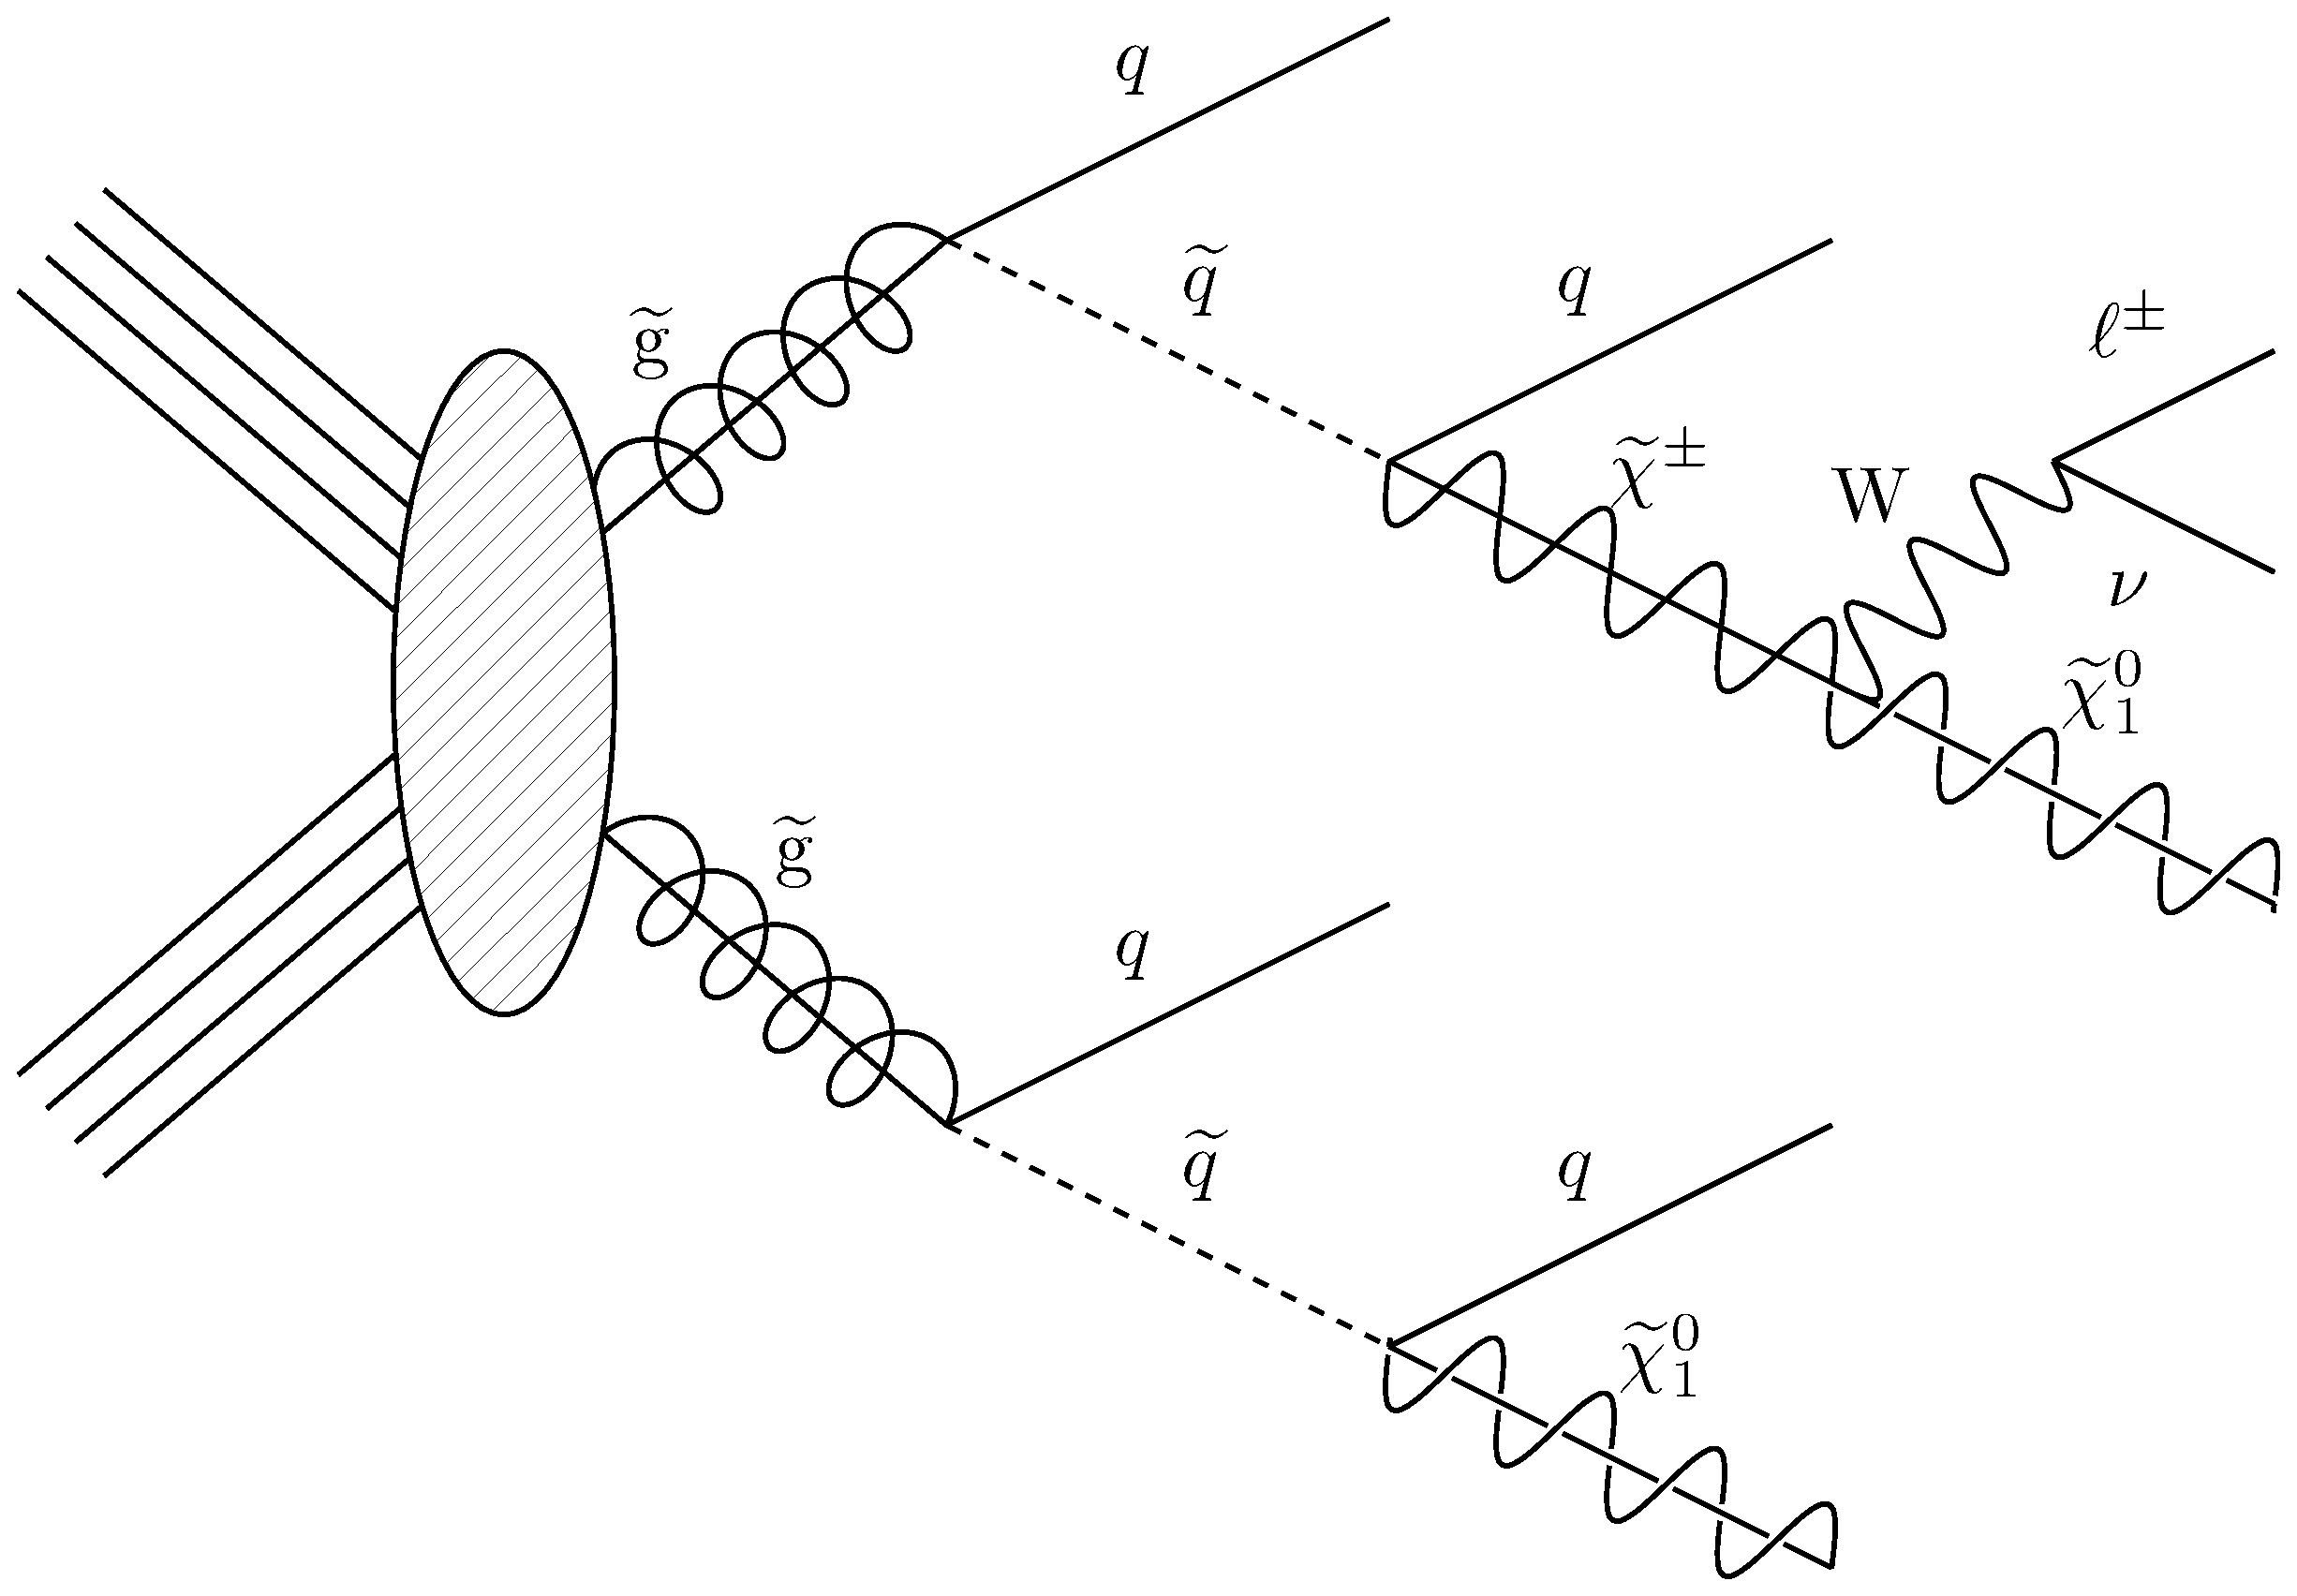
\includegraphics[width=0.7\textwidth]{fig/susy_1lep}
\caption[\ac{SUSY} decay chain leading to a single lepton final state]{Diagram
  showing a possible \ac{SUSY} decay chain beginning with gluino pair-production
  and leading to a single lepton final state.}
\label{fig:susy_1lep_decay}
\end{figure}

One such cascade decay is shown in \fig~\ref{fig:susy_1lep_decay}. This would be
a typical cascade decay leading to a single-lepton final state. Whilst being
less inclusive than the pure jets plus missing energy signature, the addition of
a lepton requirement serves to significantly suppress the experimental
background from \ac{QCD} events~\cite{msugra_signals}. With additional kinematic
requirements imposed, this channel is sensitive to a range of \ac{SUSY}
scenarios. A search based on this final state will be presented in
\chap~\ref{sec:susysearch}.

  \chapter{Theoretical Framework}
\label{sec:framework}
The previous two chapters have given a theoretical overview of the \ac{SM} and
\ac{SUSY}. In order to bring the predictions of these theories closer to the
realm of experiment, this chapter will provide a higher-level discussion more
suited to the results that will be presented later on.

A brief account of vector boson production at a hadron collider is given in
\sec~\ref{sec:framework_wpol}, along with details of the polarisation of \PW
bosons at the \ac{LHC}. This motivates the measurement described in
\chap~\ref{sec:wpol} and forms the framework within which the experimental
results will be interpreted.

In the second part of this chapter, several models relevant to \ac{SUSY}
searches will be presented. These contain a relatively low-dimensional parameter
space, making them convenient for the interpretation of experimental
results. This will be highly relevant to \chap~\ref{sec:interpretation}, where
the models will be applied to the results of the \ac{SUSY} search presented in
Chapter~\ref{sec:susysearch}.

\section[W Polarisation]{Polarisation of \PW Bosons}\label{sec:framework_wpol}
Some theoretical background relating to the \ac{SM} has been presented in
\sec~\ref{sec:sm}. Here, theoretical material relating to massive vector boson
production at hadron colliders will be briefly summarised. Then material
relating specifically to the polarisation of \PW bosons will be covered in
detail.

\subsection{Vector Boson Production at Hadron Colliders}
\label{sec:framework_vboson}
A detailed account of massive vector boson production at hadron colliders can be
found in~\cite{nadolsky, pink_book}. These processes are often referred to as
\Wjets and \Zjets -- meaning production of a \PW or \PZ boson in association
with jets. At hadron colliders, production proceeds predominantly via
$\Pquark\APquark$ or $\Pquark\Pgluon$ interactions and so is strongly dependent
on \ac{QCD} calculations. Cross-sections can be calculated as the product of the
hard scattering cross-section, evaluated in perturbative \ac{QCD}, with a
\ac{PDF}.

The \ac{PDF} is a probability density function giving the probability of finding
a certain parton with a given fraction of the longitudinal momentum, $x$, as a
function of the momentum transfer, $Q^2$. It is obtained from a fit of a
parameterised model to hadronic data. Cross-section calculations for these
processes may be referred to as \acf{LO} or \acf{NLO} This indicates the
precision of the calculation in terms of the expansion of the strong coupling
constant, \alphas~\cite{ellis_wp3jet}.

These processes have been extensively studied and significant recent progress
made, particularly for calculation of higher jet multiplicity
observables~\cite{berger_left_handed_w,berger_nlo_qcd_wjet}. The \Wjets
cross-section has been calculated at \ac{NLO} for up to 4
jets~\cite{berger_wp4jet}. The discussion will now turn to aspects relevant to
\Wjets production and in particular the polarisation effects.

\subsection{Polarisation Effects Parallel to the Beam Line}
For small values of \PW transverse momentum, \PtW, the differential angular
cross-section for the process
$\Pp\Pp\longrightarrow\PWpm\longrightarrow\Plpm\Pgnl$ follows the Drell-Yan
distribution,
\begin{equation*}
\frac{dN}{d(\cos\theta)} \propto (1\mp \cos\theta)^2.
\end{equation*}

It is well known from straightforward helicity arguments~\cite{mirkes_w_1994}
that \PW bosons produced along the beam axis will exhibit a 100\% left-handed
polarisation. This can be seen by considering the leading order partonic
subprocesses,
\begin{equation*}
\Pup\APdown \longrightarrow \PWp \qquad\textrm{and}\qquad
\Pdown\APup\longrightarrow\PWm.
\end{equation*}
Firstly, note that in the case of valence quarks, the fraction of the proton
momentum carried by the quark (as determined by the \aclp{PDF}) is greater than
that of the anti-quark. In addition given that the \ac{LHC} is a $\Pp\Pp$
collider, valence anti-quarks are not present. Anti-quarks must be drawn from
the sea and are therefore likely to be low momentum. Taking these two facts
together, the quark is very likely to have higher momentum than the
anti-quark. By momentum conservation, it is expected that the \PW boson will be
produced overwhelmingly in the direction of the original quark. Then, given the
\VminusA nature of the weak interaction (see \sec~\ref{sec:sm_electroweak}), it
is seen that the quark must be left-handed. Therefore, by helicity conservation,
the \PW will be polarised nearly 100\% left-handedly along the beam axis. A
small dilution will occur in instances where the anti-quark has, by chance, a
larger momentum fraction than the quark.

It is worth mentioning that the situation is not identical at the Tevatron
$\Pp\Pap$ collider. Although the \PWp also possess a 100\% left-handed
polarisation along the beam-line (via similar arguments to those given above),
the \PWm are found to have a near 100\% right-handed polarisation. This is a
result of the subprocess $\APup\Pdown\longrightarrow\PWm$ where this time the
\APup carries more momentum.

% TODO: Mention the effect this has on the rapidity distribution

\subsection{Polarisation Effects in the Transverse Plane}
\label{sec:polarisation}
In the case, where the \PW boson carries a significant transverse momentum, the
situation is more complex. For the sake of this discussion we will consider
cases involving only a single associated jet. Also, in order to simplify
matters, one need only consider the \PWp case, as the \PWm case is very
similar. At leading order, three subprocesses should be
considered~\cite{berger_left_handed_w},
\begin{equation}
\label{eqn:w1jet_processes}
\Pup\Pgluon\longrightarrow\PWp\Pdown\;\textrm{,} \qquad
\Pup\APdown\longrightarrow\PWp\Pgluon\qquad\textrm{and} \qquad
\Pgluon\APdown\longrightarrow\PWp\APup.
\end{equation}
For sufficiently large \PtW, the soft gluon enhancement of
$\Pup\APdown\longrightarrow\PWp\Pgluon$ and the quark-gluon subprocess is found
to dominate. It has been found that 70-80\% of $\PW+N$~jet ($N \leq 4$)
production at \ac{LO} is initiated by this subprocess.

For the quark-gluon subprocess, the $s$ and $t$-channel diagrams are shown in
\fig~\ref{fig:w1jet_st}. For the $s$-channel diagram, the on-shell \Pdown quark
is coupled directly to the \PW and therefore must be in a negative helicity
state (i.e. left-handed). Assuming a positive helicity for the W boson (as
depicted in \fig~\ref{fig:w1jet_st_s}), the spin along the $\PW\Pdown$ axis is
$1+\frac{1}{2} = \frac{3}{2}$. Such a configuration is not allowed for the
\spinhalf off-shell quark and thus the $s$-channel must lead to a 100\%
left-handed polarisation of the \PW.

In contrast, the $t$-channel diagram is not similarly constrained by spin
arguments (since the \PW is not coupled directly to the quark) and thus the
polarisation will not be seen. It can be shown that, for a left-handed incoming
gluon, the $t$-channel diagram can be made to
vanish~\cite{berger_left_handed_w}. Also, for a right-handed gluon, the \PW
polarisation is not constrained, but has been shown to become predominantly
right-handed at high \PtW. The helicity of the outgoing \PW will be almost 100\%
correlated with that of the incoming gluon at high \PtW.

Overall, due to a factor 4 difference in the size of the corresponding matrix
elements, the \PW is expected to asymptotically approach an 80\% left-handed
polarisation at large \PtW. The \VminusA coupling allows the decay leptons to be
used as an analyser of the \PW polarisation. This allows the effect to be
measured. Having given an overview of the physics underlying this effect, a more
detailed argument will now be presented.

\begin{figure}[h!]
\centering
\subfloat[]{\label{fig:w1jet_st_s}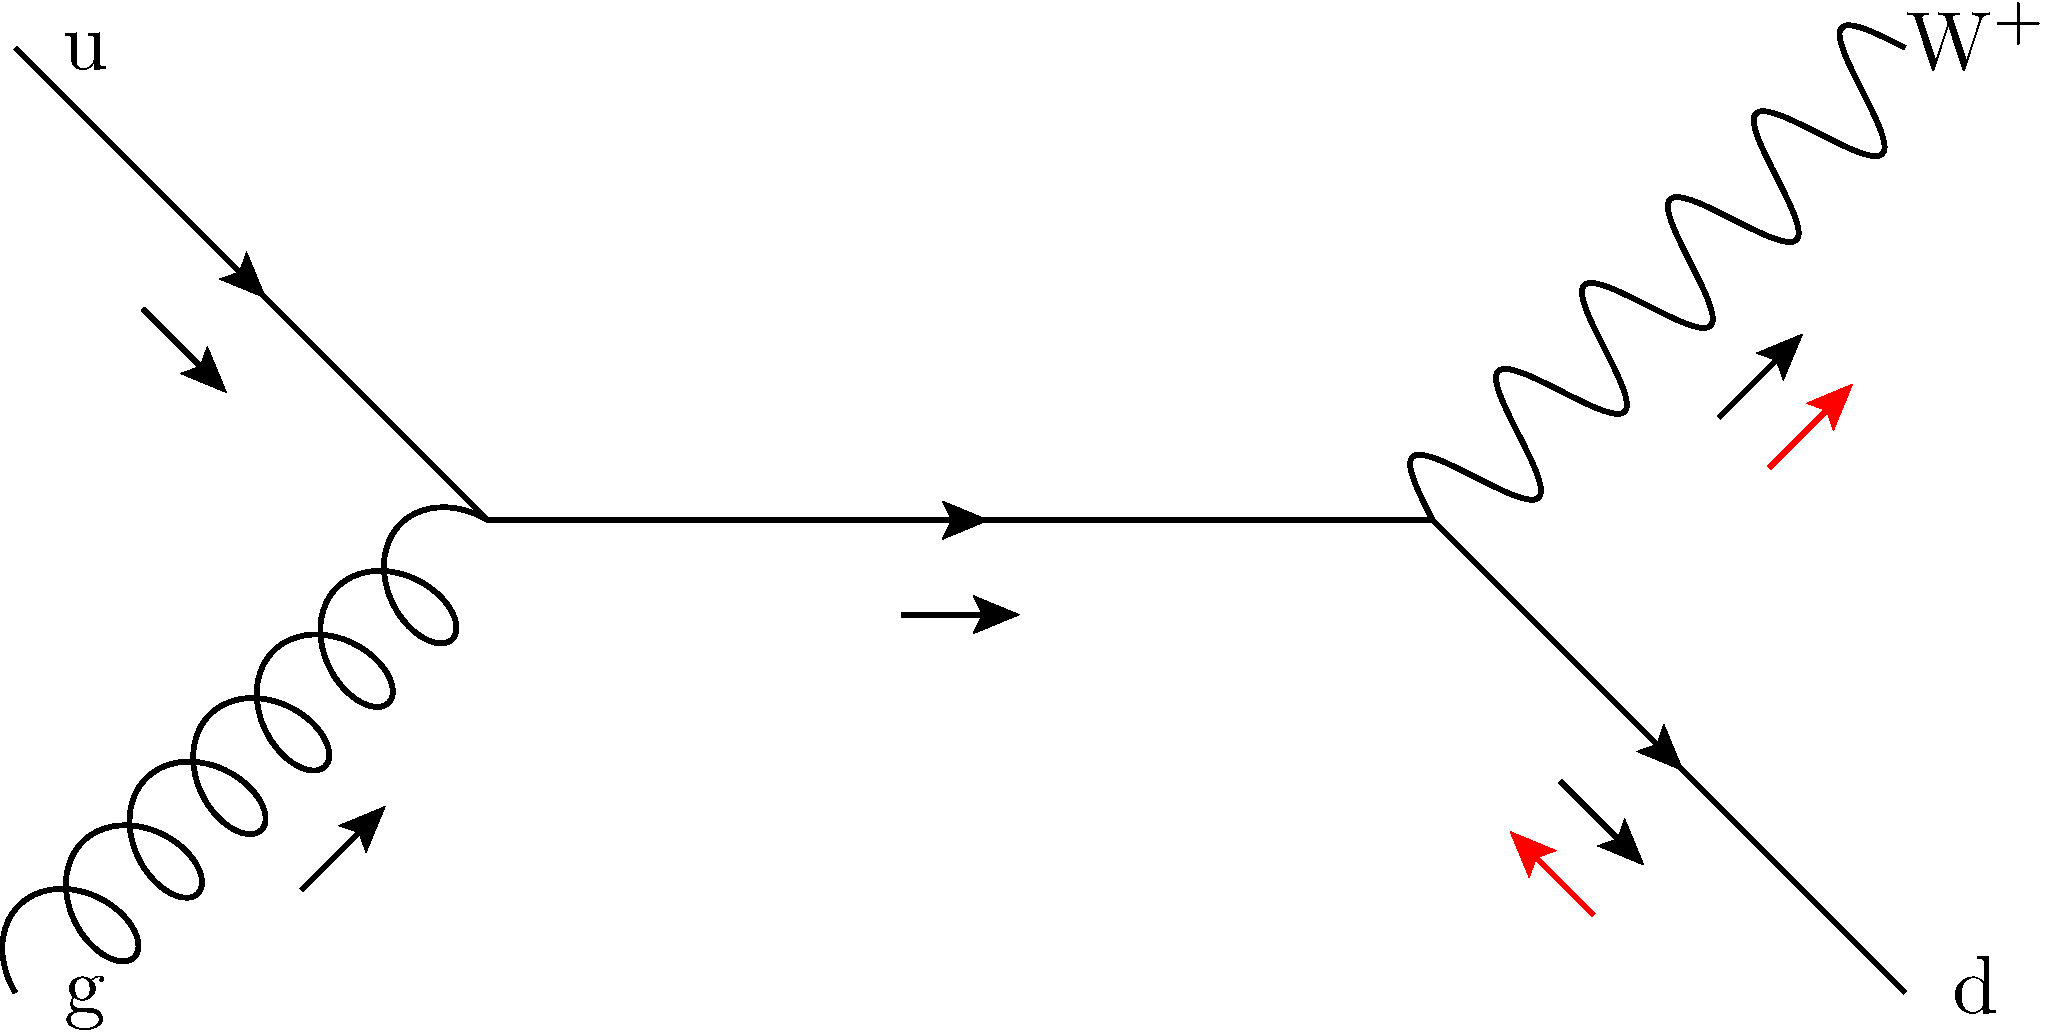
\includegraphics[width=0.5\textwidth]{fig/wpol_1jet_s}}\quad
\subfloat[]{\label{fig:w1jet_st_t}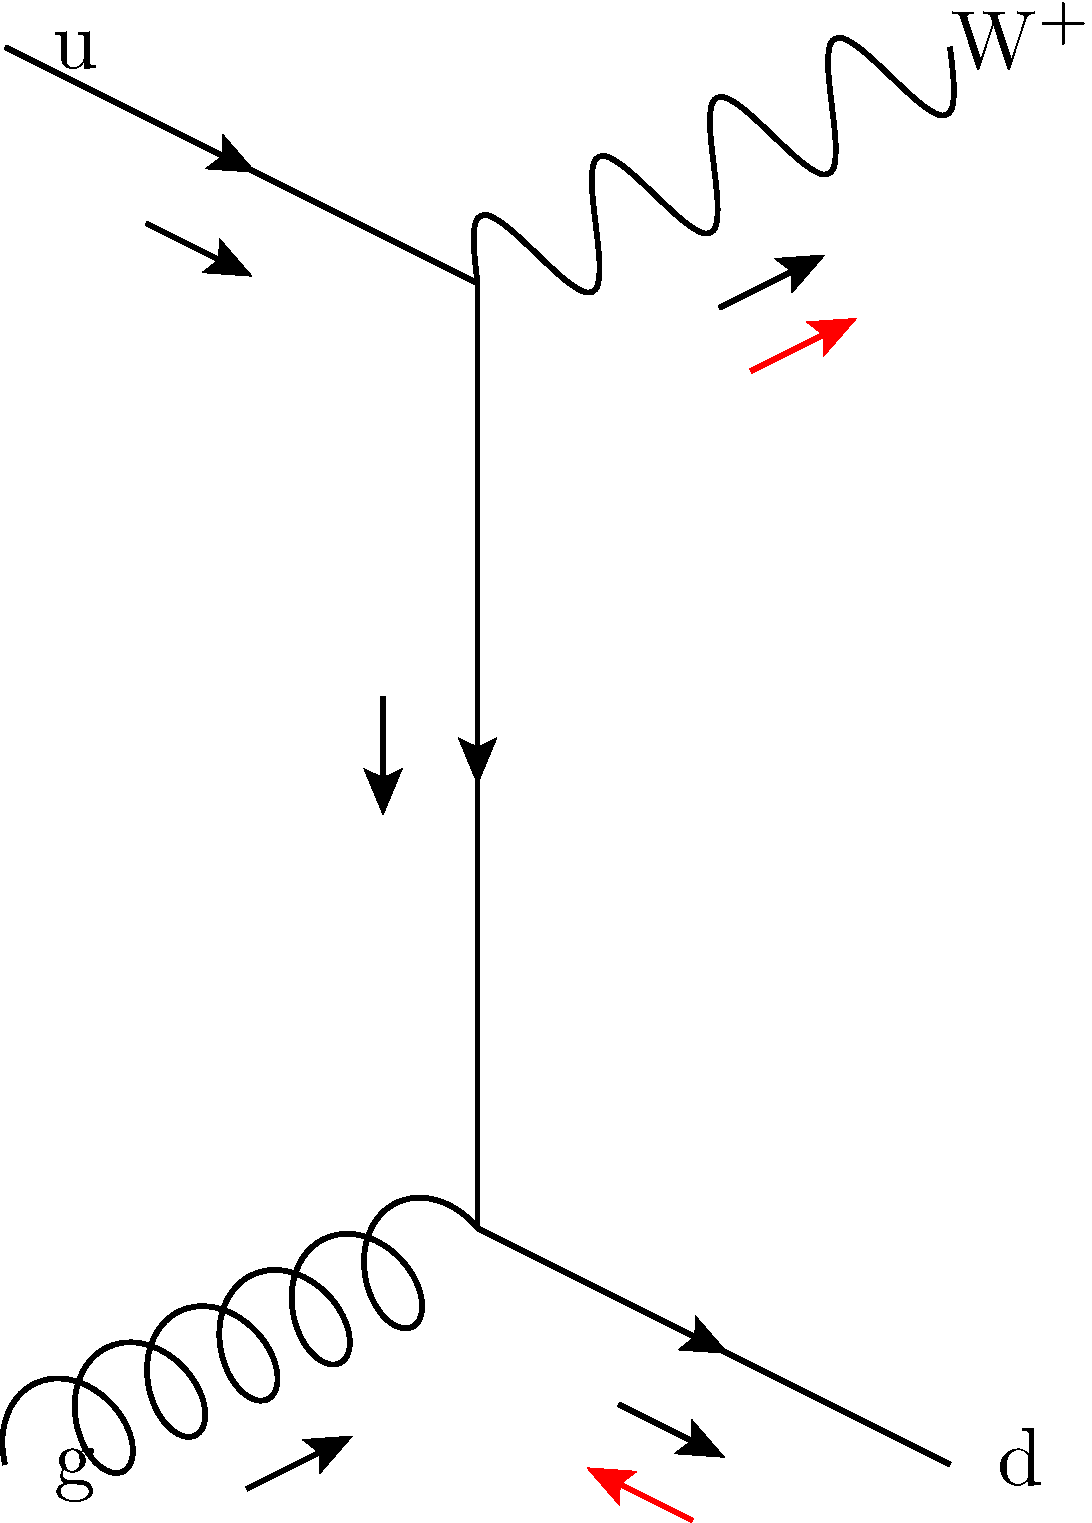
\includegraphics[width=0.25\textwidth]{fig/wpol_1jet_t}}
\caption[Diagrams showing the $\Pup\Pgluon\longrightarrow\PWp\Pdown$
subprocess]{Diagrams showing the $\Pup\Pgluon\longrightarrow\PWp\Pdown$
  subprocess in the \subref{fig:w1jet_st_s} $s$ and \subref{fig:w1jet_st_t} $t$
  channels. The black displaced arrows indicate the particle momenta. For the
  $s$ channel diagram, the helicity vectors are shown as red arrows, for the
  case of a right-handed \PW boson.}
\label{fig:w1jet_st}
\end{figure}

Writing the amplitudes of the subprocesses in \eqn~\ref{eqn:w1jet_processes}
in terms of spinor products, two distinct expressions emerge,

\begin{eqnarray*}
\mathcal{A}^{\textrm{tree}}_{(a)} &\propto&
\frac{\left<\Pdown\nu\right>^2}{\left<\Pup\Pgluon\right>\left<\Pgluon\Pdown\right>} \textrm{and}\\
\mathcal{A}^{\textrm{tree}}_{(b)} &\propto&
\frac{\left[\Pup\Pe\right]^2}{\left[\Pup\Pgluon\right]\left[\Pgluon\Pdown\right]},
\end{eqnarray*}
where factors common to both expressions are not shown. The corresponding
cross-sections are
\begin{equation}
\label{eqn:w1jet_xs}
d\sigma^{\textrm{LO}}_{(a)} \propto (k_{\Pdown} \dot k_{\Pneutrino})^2 \quad \textrm{and} \quad
d\sigma^{\textrm{LO}}_{(b)} \propto (k_{\Pup} \dot k_{\Pe})^2,
\end{equation}
where the $k$ are Lorentz vectors representing the particle momenta. For each
subprocess, the helicity configurations corresponding to $(a)$ and $(b)$ are
shown in the upper and lower rows of \fig~\ref{fig:w1jet_modes}
respectively. The red arrows indicate particle helicity, with a double-stemmed
arrow for the \PW momentum. In the cases where the \PW boson is neither purely
left-handed nor right-handed, the arrow is placed at an angle.

Starting with the subprocess $\Pup\Pgluon\longrightarrow\PWp\Pdown$, the $(a)$
expression in \ref{eqn:w1jet_xs} correlates the axis of the \Pdown quark with
the neutrino. This is shown in \fig~\ref{fig:w1jet_modes_1a}. The \VminusA
coupling requires the neutrino to have a left-handed helicity. By angular
momentum conservation, the \PW boson must also be left-handed. The angular
dependence is $(1-\cos\tilde{\theta}^*)^2$ where $\tilde{\theta^*}$ is the angle
of the charged decay lepton with respect to the \PW flight direction in the
centre-of-mass frame. In contrast, consider an identical particle configuration,
but with helicities corresponding to $(b)$. This is shown in
\fig~\ref{fig:w1jet_modes_1b}. The \Ppositron direction is now correlated with
the incoming beam direction. Boosting to the \PW rest frame, at high \PtW, the
incoming quark and gluon are nearly parallel. Thus, given a scattering angle of
90\degrees, the \Pup quark momentum is seen to be half that of the \Pdown
quark. The angular dependence is thus $\frac{1}{4}(1+\cos\tilde{\theta}^*)^2$,
yielding a right-handed polarisation at a quarter of the rate of the left-handed
component.

For the sub-dominant process $\Pup\APdown\longrightarrow\PWp\Pgluon$, the terms
in \eqn~\ref{eqn:w1jet_xs} correlate the momenta of the decay leptons with the
beam direction. The two cases are shown in \figs~\ref{fig:w1jet_modes_2a} and
\ref{fig:w1jet_modes_2b}. Although it can be seen once again that a left-handed
and right-handed polarisation emerge, in this case they are found to cancel for
a scattering angle of 90\degrees and thus give no net polarisation
effect. Lastly, for the subprocess $\Pgluon\APdown\longrightarrow\PWp\APup$,
shown in \figs~\ref{fig:w1jet_modes_3a} and \ref{fig:w1jet_modes_3b}, the $(b)$
contribution correlates the \Pup quark and the \Ppositron direction, leading to
a dominantly right-handed polarisation. However, since the \ac{PDF},
$\APdown(x)$, is much smaller than $\Pup(x)$, this effect is largely washed out
by the dominant left-handed polarisation mode.

\begin{figure}[h!]
\centering
\subfloat[]{\label{fig:w1jet_modes_1a}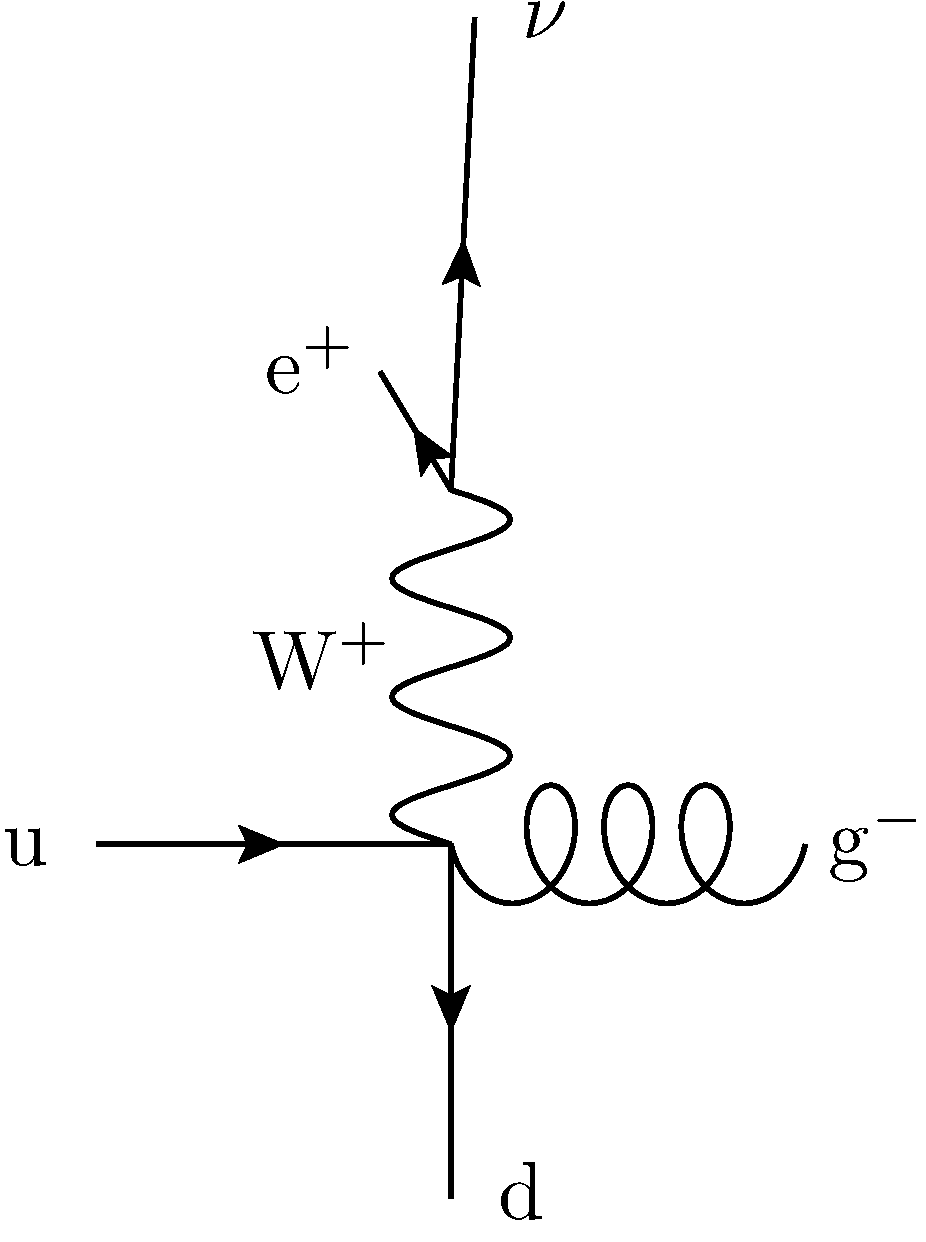
\includegraphics[width=0.3\textwidth]{fig/wpol_prod_a}}\quad
\subfloat[]{\label{fig:w1jet_modes_2a}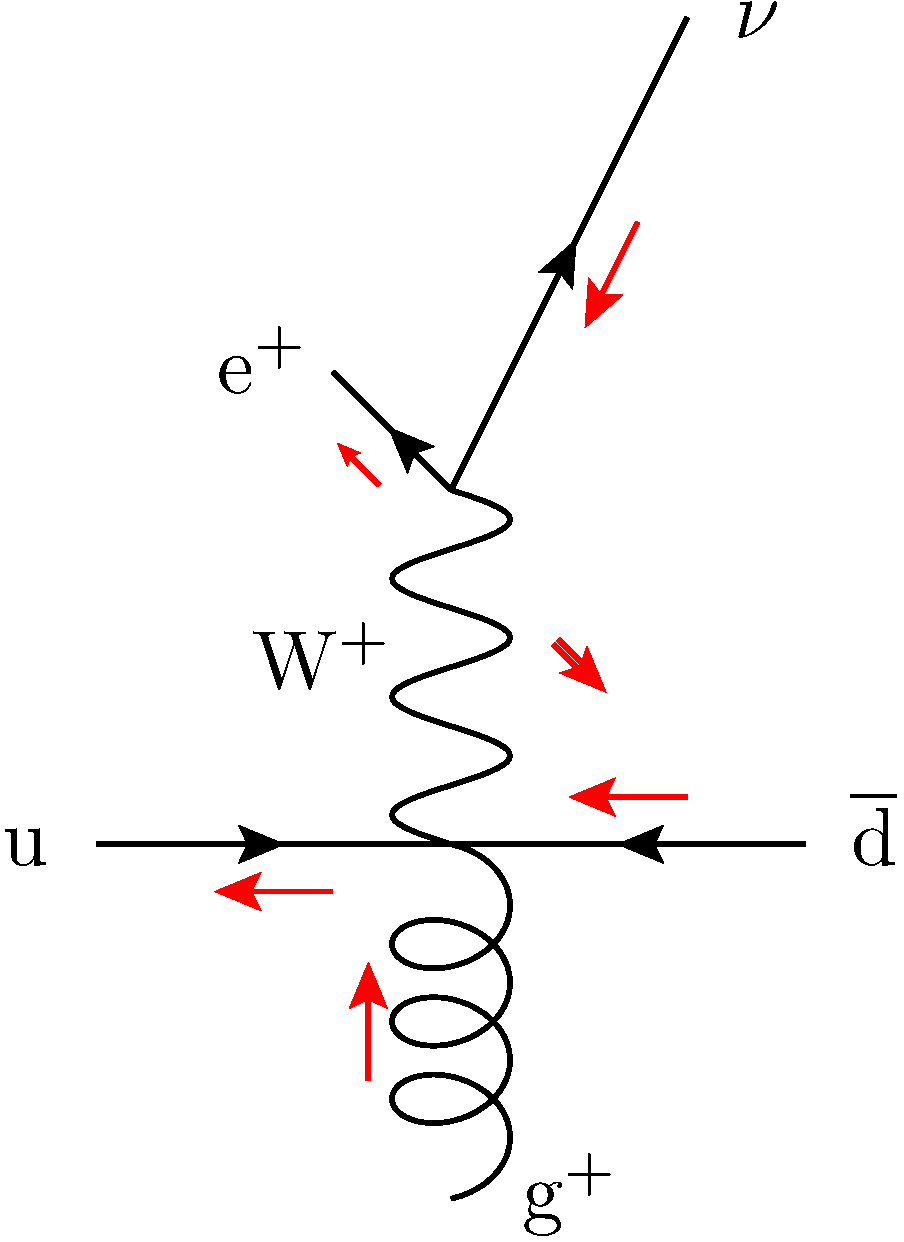
\includegraphics[width=0.3\textwidth]{fig/wpol_prod_b}}\quad
\subfloat[]{\label{fig:w1jet_modes_3a}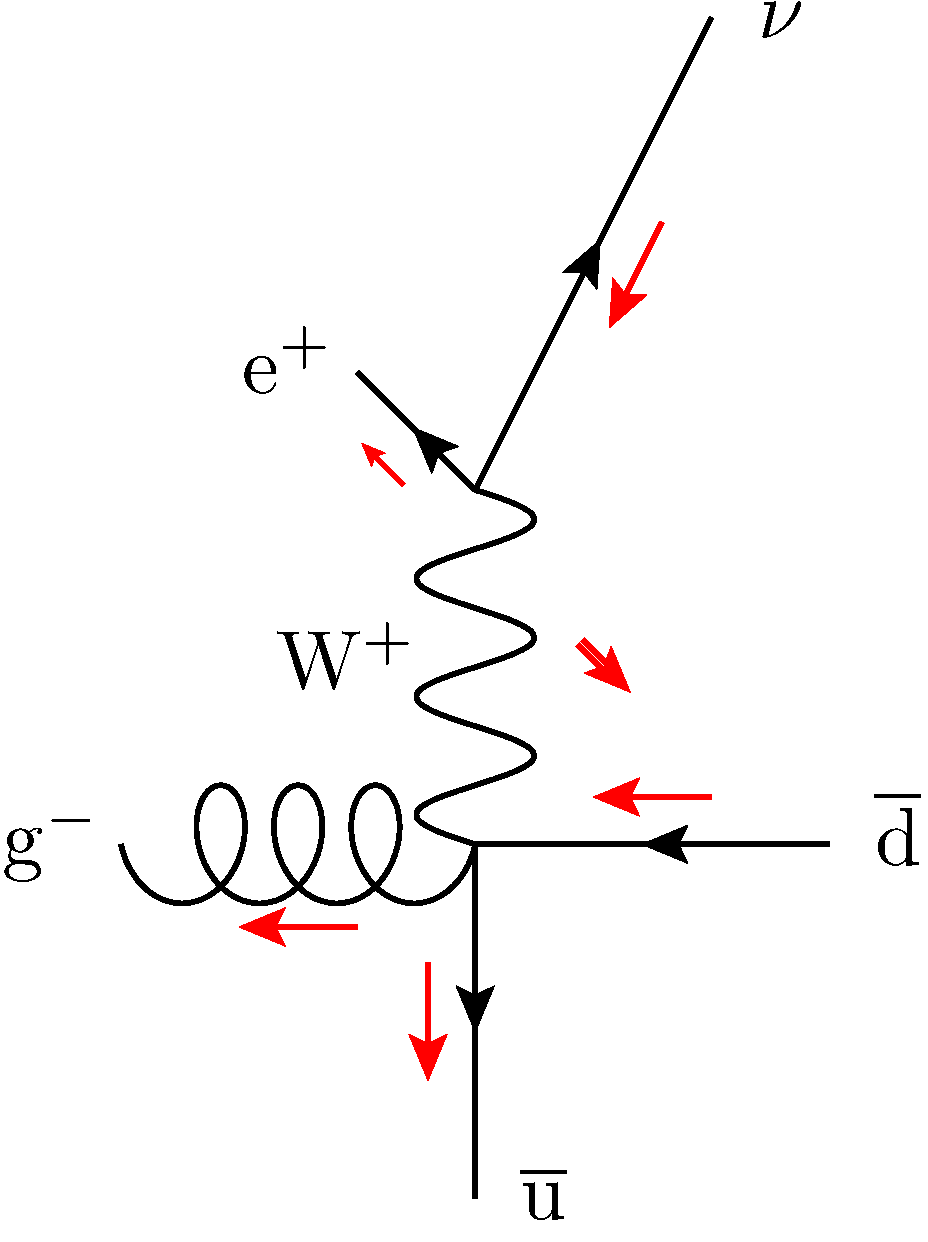
\includegraphics[width=0.3\textwidth]{fig/wpol_prod_c}}\\
\subfloat[]{\label{fig:w1jet_modes_1b}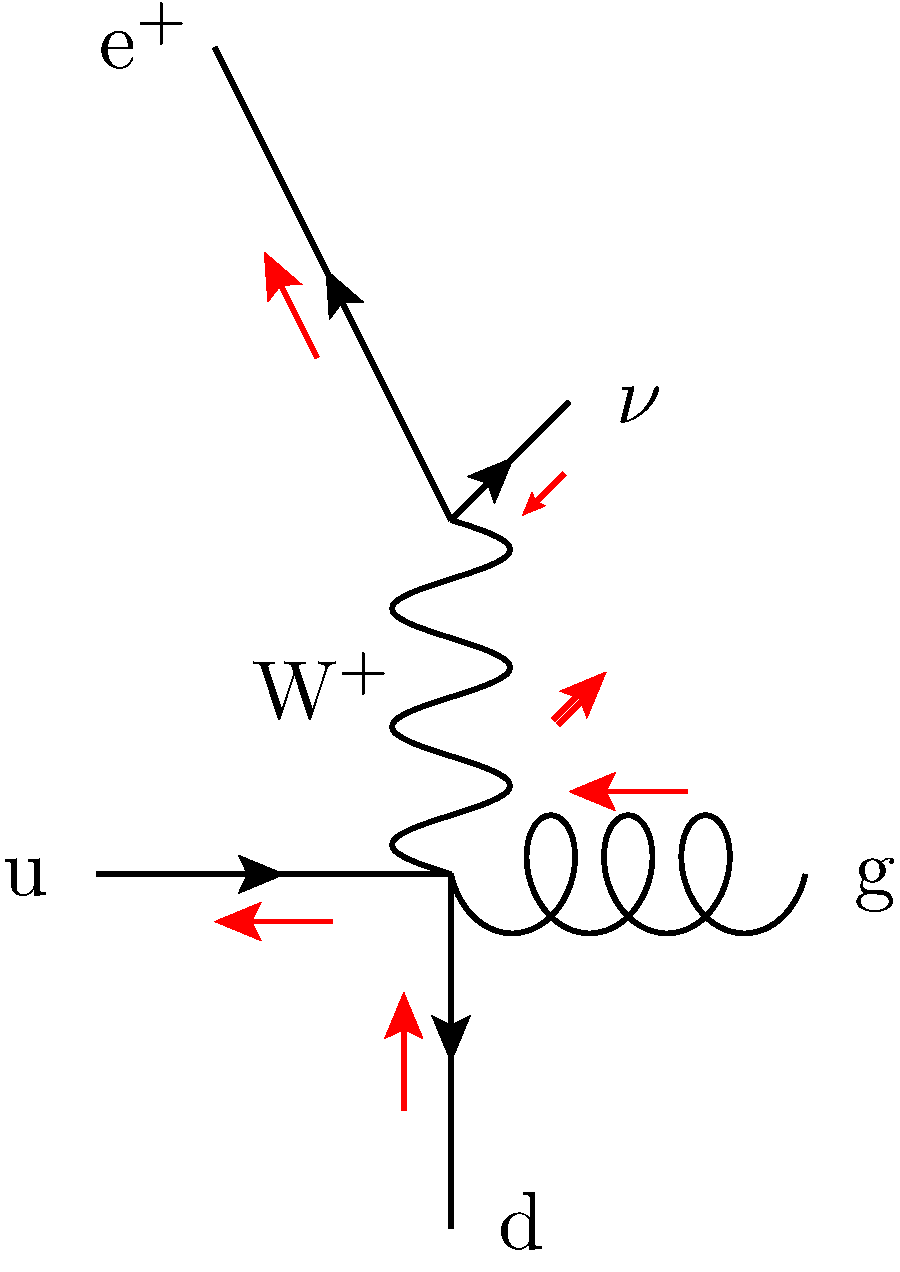
\includegraphics[width=0.3\textwidth]{fig/wpol_prod_d}}\quad
\subfloat[]{\label{fig:w1jet_modes_2b}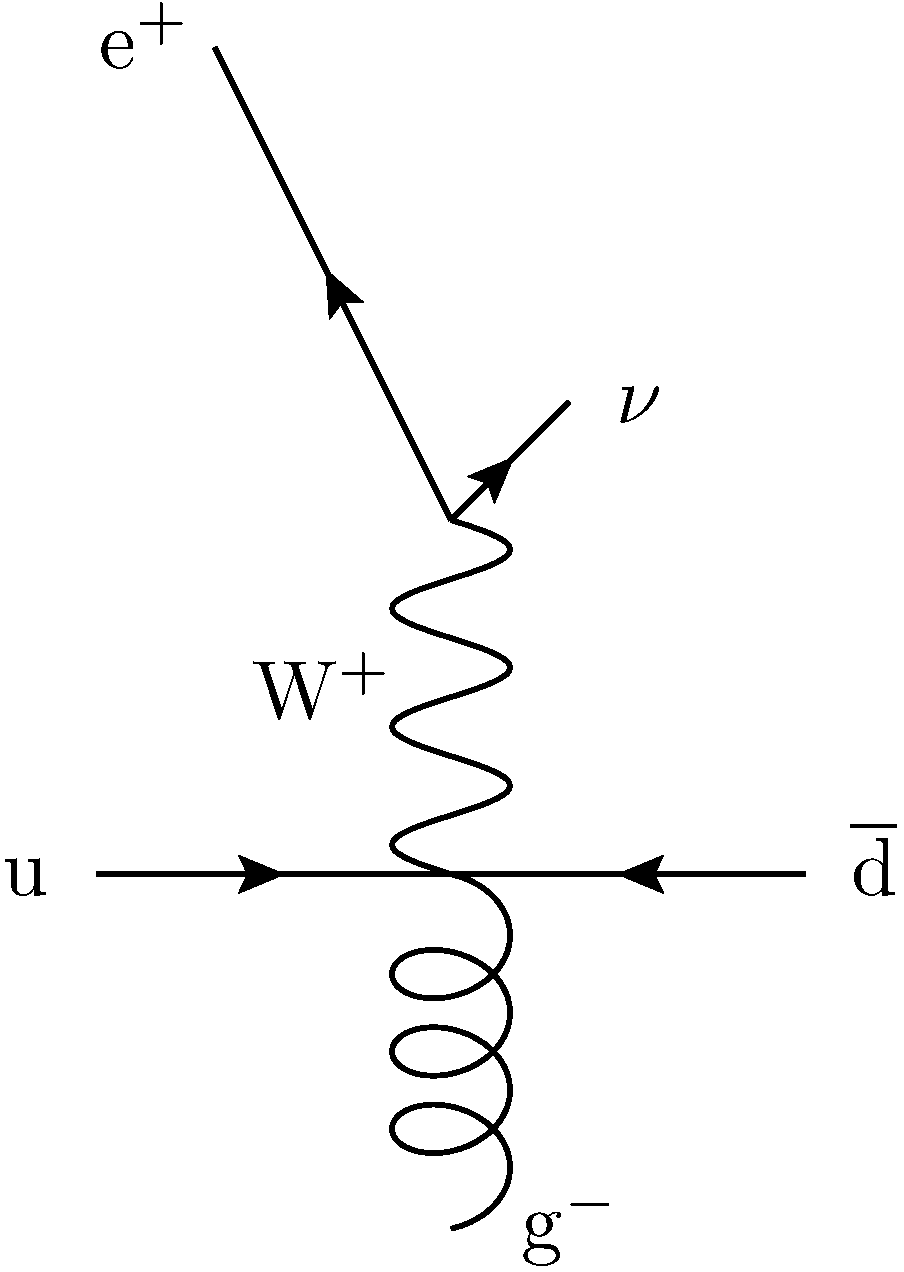
\includegraphics[width=0.3\textwidth]{fig/wpol_prod_e}}\quad
\subfloat[]{\label{fig:w1jet_modes_3b}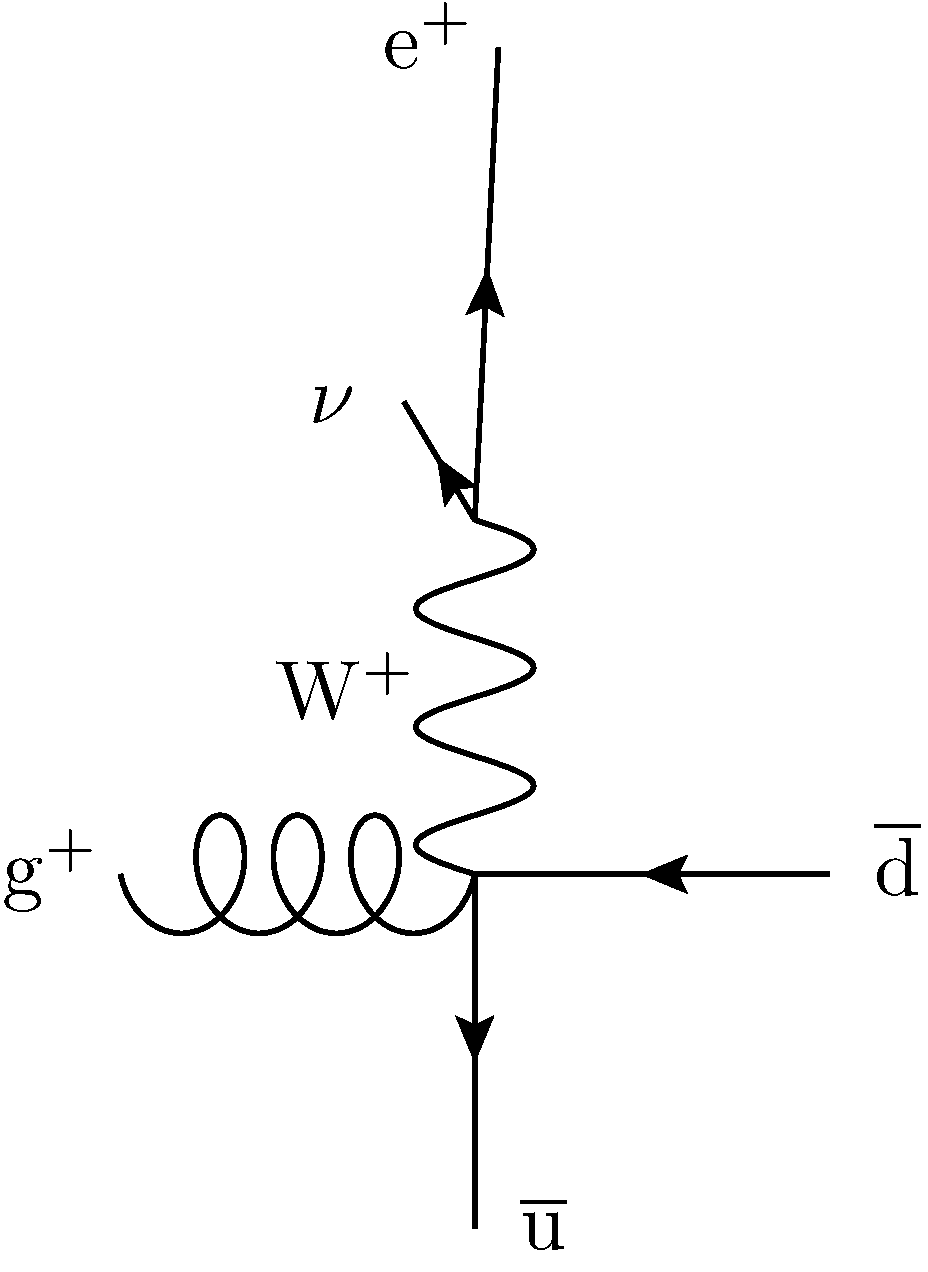
\includegraphics[width=0.3\textwidth]{fig/wpol_prod_f}}
\caption{Illustrations of $\PWplus+1$~jet production modes at the LHC. Red
  single-stemmed arrows represent particle helicity. Red double-stemmed arrows
  indicate the polarisation of the \PW boson. In cases where the \PW is not
  produced with a definite polarisation, the arrow is placed at an angle. The
  angles and sizes of the particle lines are suggestive of their momenta in the
  centre-of-mass frame.}
\label{fig:w1jet_modes}
\end{figure}

It has been seen that the proton-proton environment at the \ac{LHC} is expected
to lead to a dominance of left-handed over right-handed helicity states for \PW
bosons with large transverse momentum. In order to observe this effect, the
helicity of \PW bosons must be measured. This will be discussed in the next section.

\subsection{Measuring Helicity}
\subsubsection{The Helicity Frame}
Polarisation effects may be conveniently studied within the helicity frame of
the \PW boson. This is illustrated in \fig~\ref{fig:wpol_helicity_frame}. The
helicity frame is defined in the rest frame of the \PW boson, with the
polarisation axis (here, the z-axis) aligned along the \PW line-of-flight in the
lab frame. The x-axis is then chosen to lie along the plane spanned by the two
colliding protons in the boson rest frame. The sense is chosen such that the
angle between the axis and the nearest proton is minimised. The y-axis is then
fixed to be perpendicular to these two (the coordinate system is
right-handed). The polar angle, \thetastar is measured in the $y-z$ plane
between the positive z-axis and the lepton. Likewise, the azimuthal angle,
\phistar is measured in the $x-z$ plane, between the positive $x$ axis and the
lepton. For $0 < |\phistar| < \frac{\pi}{2}$, the charged lepton will have a
larger rapidity that the \PW boson and thus a smaller \Pt. Alternatively, for
$\frac{\pi}{2} < |\phistar| < \pi$, the lepton will have a smaller rapidity and
a larger \Pt.

\begin{figure}[h!]
%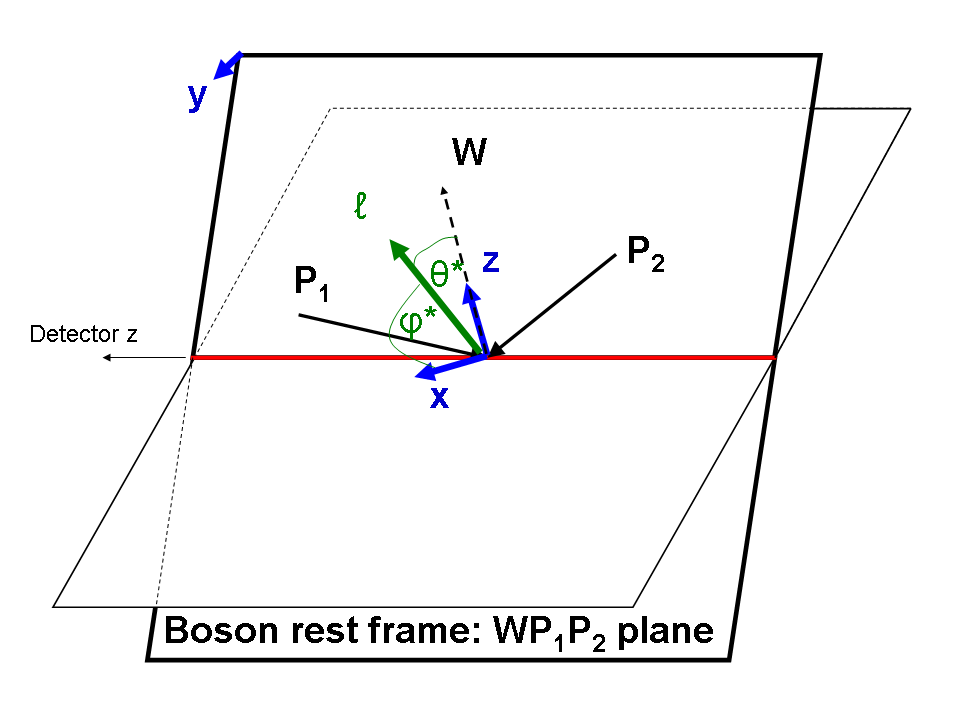
\includegraphics[width=0.8\textwidth]{fig/helicity_frame_polnote}
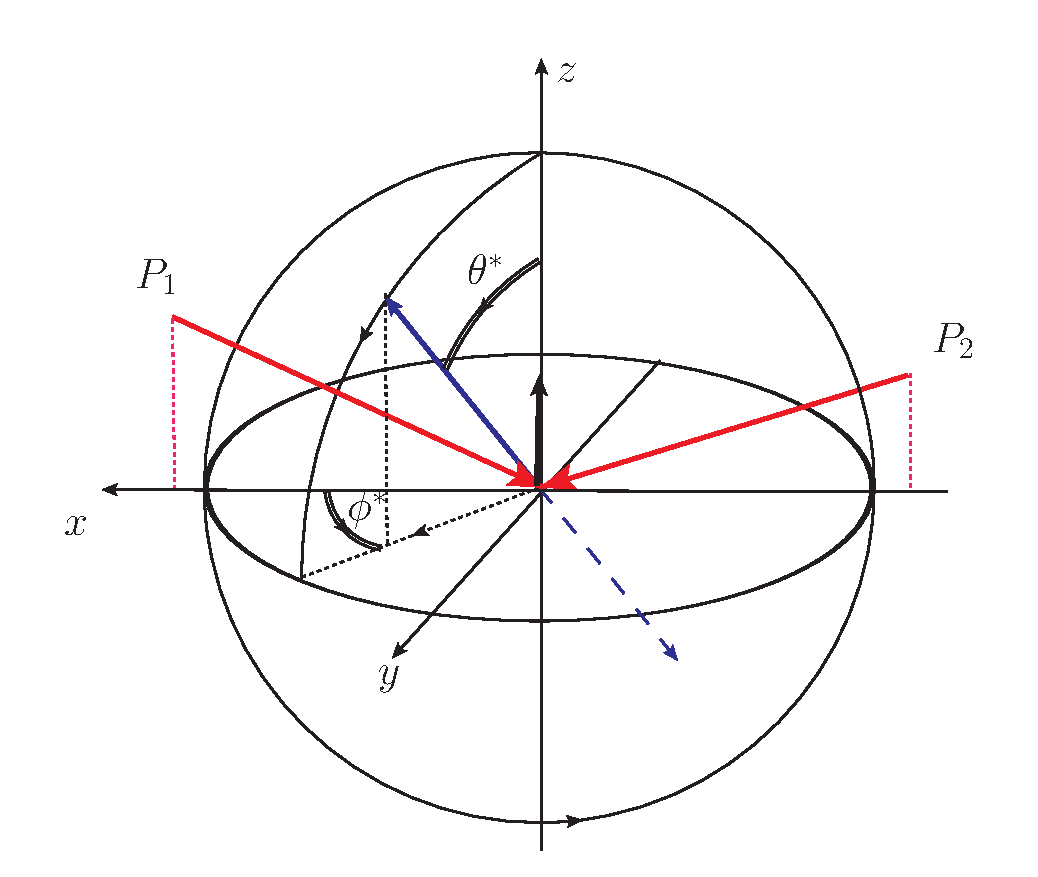
\includegraphics[width=0.8\textwidth]{fig/helicity_frame_better}
\caption[The Helicity Frame]{The Helicity Frame~\cite{berger_left_handed_w}}
\label{fig:wpol_helicity_frame}
\end{figure}

\subsubsection{Quantifying Helicity}
\label{sec:quant_helicity}
The hadronic cross-section of the \PW is obtained within the parton model by
weighting the individual parton-level cross-sections with the respective
\acp{PDF}~\cite{mirkes_w_1994},
\begin{equation*}
\frac{d\sigma^{h_1 h_2}}{d(\PtW)^2 dy d\Omega^*} = \sum_{ab} \int dx_1 dx_2
f_a^{h_1}\left(x_1, \mu_F^2\right)f_b^{h_2}\left(x_2, \mu_F^2\right)
\times \frac{s d\tilde{\sigma}_{ab}}{dt du d\Omega^*} \left(x_1 P_1, x_2 P_2,
\alpha_s (\mu_R^2)\right),
\end{equation*}
where $h_1$ and $h_2$ are the interacting hadrons and the sum runs over $a,b =
\Pquark, \APquark, \Pgluon$. The \acp{PDF}, $f_a^{h}\left(x, \mu^2\right)$, give
the probability of finding a parton $a$ with momentum fraction $x$ in hadron $h$
when probed at a scale $\mu^2$. The $d\tilde{\sigma}_{ab}$ are the parton-level
cross-sections for the chosen process(es). The hadron-level Mandelstam variables
are written in uppercase,
\begin{equation*}
S = (P_1 + P_2)^2 \qquad T = (P_1 - Q)^2 \qquad U = (P_2 - Q)^2,
\end{equation*}
and parton-level in lowercase,
\begin{eqnarray*}
s &=& (p_1 + p_2)^2 = x_1 x_2 S\\
t &=& (p_1 - Q)^2  = x_1(T-Q)^2 +Q^2\\
u &=& (p_2 - Q)^2 = x_2(U -Q)^2 + Q^2,
\end{eqnarray*}
where
\begin{equation*}
p_1 = x_1 P_1 \qquad p_2 = x_2 P_2.
\end{equation*}
The momenta of the incoming hadrons are labelled $P_1$ and $P_2$ and the
interacting partons, $p_1$ and $p_2$. This expression can be rewritten in terms
of a standard set of angular coefficient $A_i$, to give~\cite{mirkes_w_1992}
\begin{align}
\label{eqn:wpol_diff_xs}
\frac{d\sigma}{d(\PtW)^2 dy d\cos\theta d\phi} = \frac{3}{16\pi}
\frac{d\sigma^{-1}}{d(\PtW)^2 dy} &\left [ \left(1+\cos^2\theta\right) \right. \nonumber\\
 &+ \frac{1}{2} A_0 \left ( 1 - 3\cos^2\theta \right ) + A_1 \sin 2\theta\cos\phi \nonumber\\
 &+ \frac{1}{2}A_2\sin^2\theta\cos 2\phi + A_3\sin\theta\cos\phi \nonumber\\
 &+ A_4\cos\theta + A_5\sin^2\theta\sin 2\phi \nonumber\\
 &+ A_6\sin 2\theta\sin \phi + A_7\sin\theta\sin\phi
\end{align}

% TODO: Figure out the difference between  theta and theta*
The $A_i$ are ratios of the separate helicity cross-sections of the boson to its
total unpolarised cross-section. They are dependent on the \PW boson charge,
transverse momentum, \PtW, and rapidity, \YW. \eqn~\ref{eqn:wpol_diff_xs} can be
integrated over $\phi$ and \PtW to give
\begin{equation}
\label{eqn:wpol_xs_Ai}
\frac{d\sigma}{d\cos\theta} \propto \left(1+\cos^2\theta\right) +
\frac{1}{2}A_0\left(1-3\cos^2\theta\right) + A_4\cos\theta.
\end{equation}

% TODO: Check all this bs!
Again, because of the \VminusA coupling, the \PWp (\PWm) may couple only to
left-handed (right-handed) fermions and right-handed (left-handed)
anti-fermions. Therefore the angular momentum state of the decay leptons is
\begin{eqnarray*}
\ket{\Pl\Pgn^{J,M}} &=& \ket{\frac{1}{2}, \pm \frac{1}{2}}
\oplus \ket{\frac{1}{2}, \pm\frac{1}{2}} \\
&=& \textrm{either}\quad\ket{1, +1}\quad\textrm{or}\quad \ket{1, -1},
\end{eqnarray*}
where $\ket{J, M}$ represents an angular momentum state with a total angular
momentum, $J$, and projection, $M$. Rotating these states through the angle
\thetastar, one obtains
\begin{equation}
\ket{\Pl\Pgn^{J,M}}' = \sum_{M'=-J}^{M'=+J} d_{M, M'}^J \ket{J, M'}.
\end{equation}
The angular momentum of a \PW boson in a helicity eigenstate is then
$\ket{\PW^{J,M''}}$. The matrix element for the angular momentum coupling can be
written
\begin{eqnarray*}
\braket{\PW^{J,M''}}{\Pl\Pgn^{J,M}}' &\sim& \sum_{M'=-J}^{M'=+J} d_{M M'}^{J}
\braket{J,M''}{J,M'} \\
&\sim& d^{J}_{M M''} \braket{J,M''}{J,M''} \sim d_{M M''}^{J}.
\end{eqnarray*}
The cross-section is calculated by squaring the matrix elements and summing over
the helicity states ($M''$) of the incoming $\PW$ boson. Each state is weighted
by the helicity fraction $f_{M''}$,
\begin{equation*}
  \sigma(\PW\longrightarrow\Pl\Pgnl) \sim f_0 \left|d_{M 0}^1\right|^2 + f_{-1} \left|d_{M
      -1}^1\right|^2 + f_{1} \left|d_{M +1}^1\right|^2,
\end{equation*}
where $f_0 + f_1 + f_{-1} = 1$. Finally, using the fact that for \PWpm,
$M=\pm1$, and replacing for the elements of the D-matrices in terms of
$\cos\thetastar$ gives,
\begin{equation}
\label{eqn:wpol_helicity_fractions}
\sigma(\thetastar_{\Plpm}) = \frac{\f0}{2}\sin^2\thetastar_{\Plpm} +
\frac{\fL}{4} \left(1\mp\cos\thetastar_{\Plpm}\right)^2 +
\frac{\fR}{4} \left(1\pm\cos\thetastar_{\Plpm}\right)^2.
\end{equation}
Note that the helicity fractions \ffi have been relabelled to give a more
intuitive interpretation as the left-handed, right-handed and longitudinal
polarisation fractions. Comparing now to \eqn~\ref{eqn:wpol_xs_Ai}, we identify
\begin{eqnarray*}
A_0 \sim f_0 \textrm{and}\\
A_4 \sim \pm \fLmfR.
\end{eqnarray*}
Whilst the $A_i$ are the more fundamental parameters from a theoretical point of
view, the helicity fractions \f0, \fL and \fR will often be more convenient for
experimental discussion. The other \Ai parameters will not be discussed in
detail, though their small effect on the measurement of $A_0$ and $A_4$ will be
evaluated.

In \chap~\ref{sec:wpol}, the measurement of the helicity fractions \fL, \fR and
\f0 will be described. The intention of this analysis is to confirm the
prediction that the left-handed mode dominates at high \PtW, or equivalently,
$\fLmfR > 0$. In addition, it is expected that $\fL > \f0$.

The evolution of the polarisation fractions with \PtW has also been studied in
simulation~\cite{berger_left_handed_w}. The evolution of \fL, \fR and \f0 is
shown in \fig~\ref{fig:framework_ptw} for the \PWp case. The increase of \fLmfR
with \PtW can be readily seen. Also, because of the equivalence
theorem~\cite{equiv_theorem,tev_physics,gounaris,cornwall,elementary_pp}, the
behaviour of the longitudinal polarisation mode approximates the corresponding
Goldstone boson (see \sec~\ref{sec:sm_goldstone}) at large \PtW. This explains
the decrease of \f0 as \PtW becomes large.

Whilst the dependence of the polarisation on \PtW make for a very interesting
measurement, it was found to be infeasible with the relatively small data sample
available for this analysis.

\begin{figure}[h!]
\centering
\subfloat[\fL]{\label{fig:framework_ptw_fL}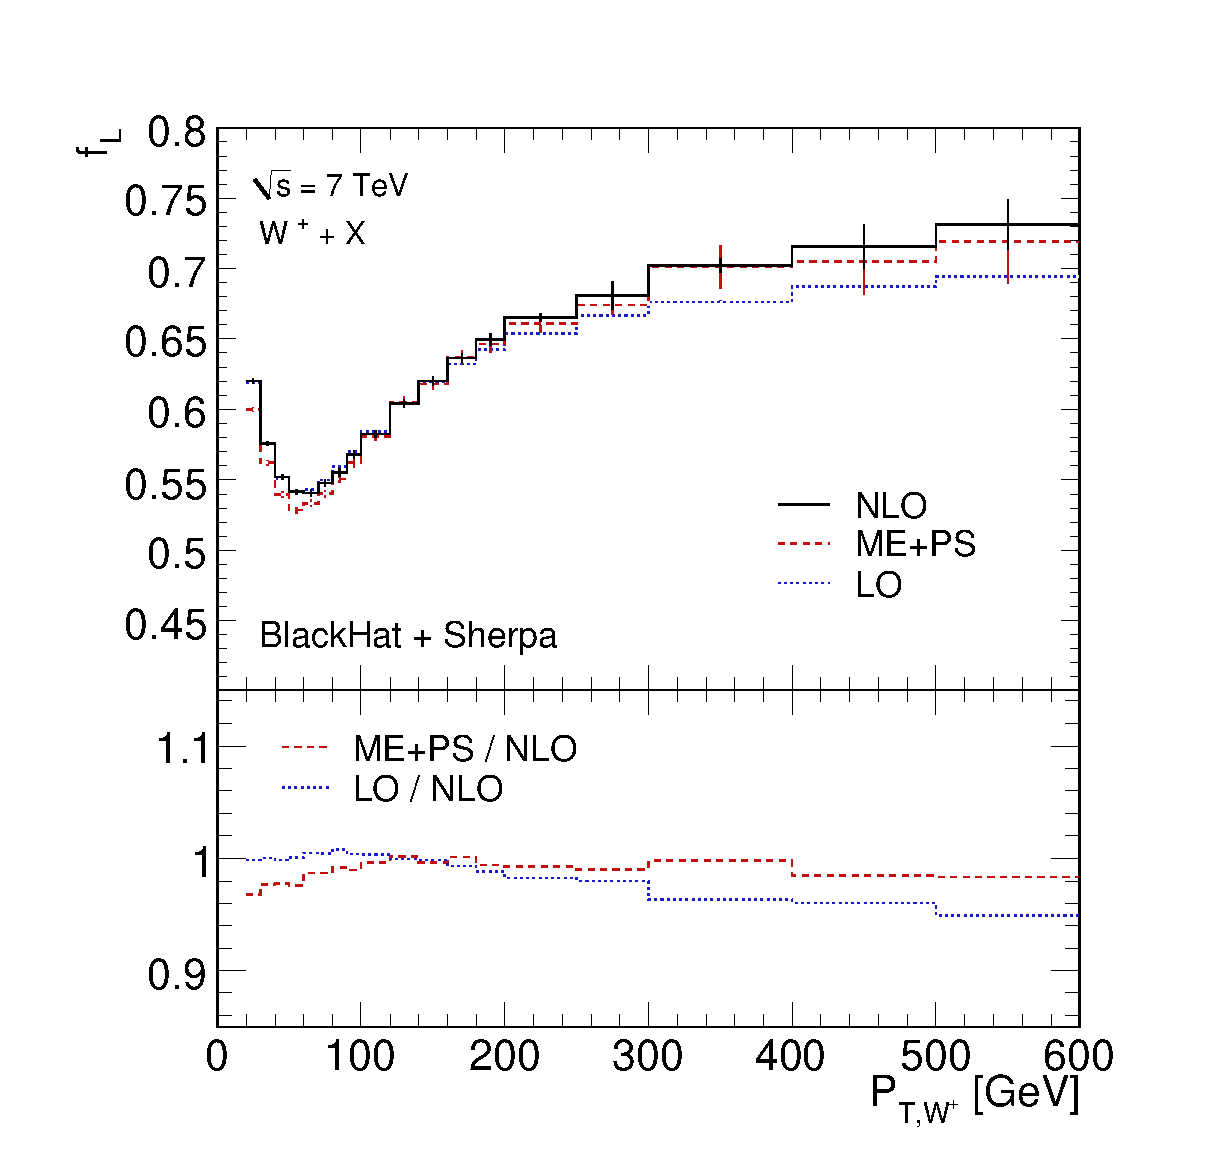
\includegraphics[width=0.29\textwidth]{fig/fL_Wp}}
\subfloat[\fR]{\label{fig:framework_ptw_fR}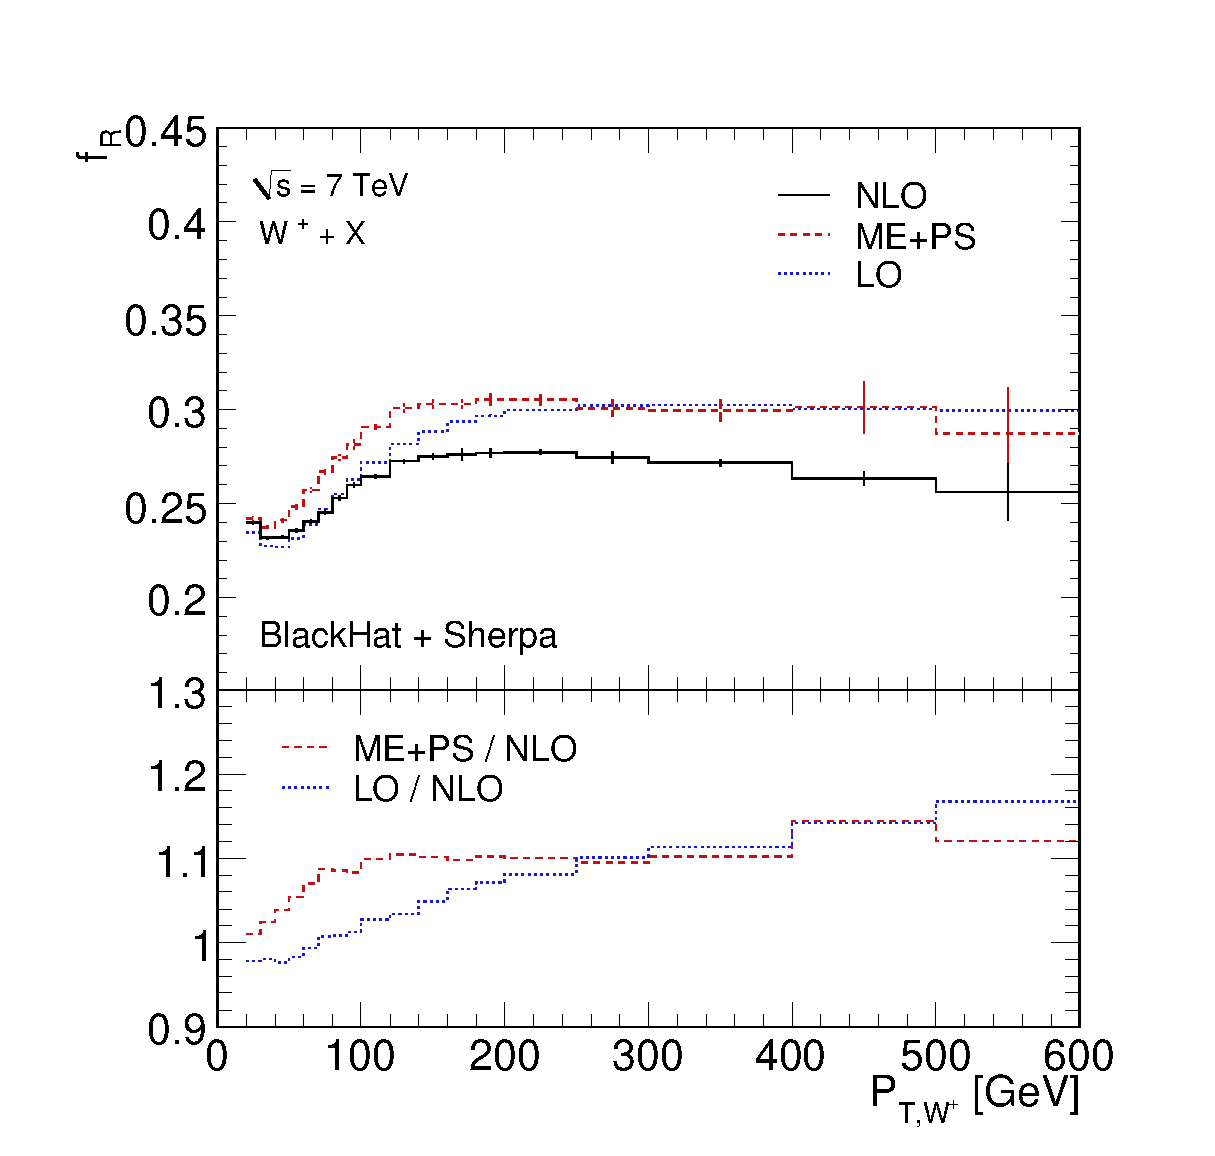
\includegraphics[width=0.29\textwidth]{fig/fR_Wp}}
\subfloat[\f0]{\label{fig:framework_ptw_f0}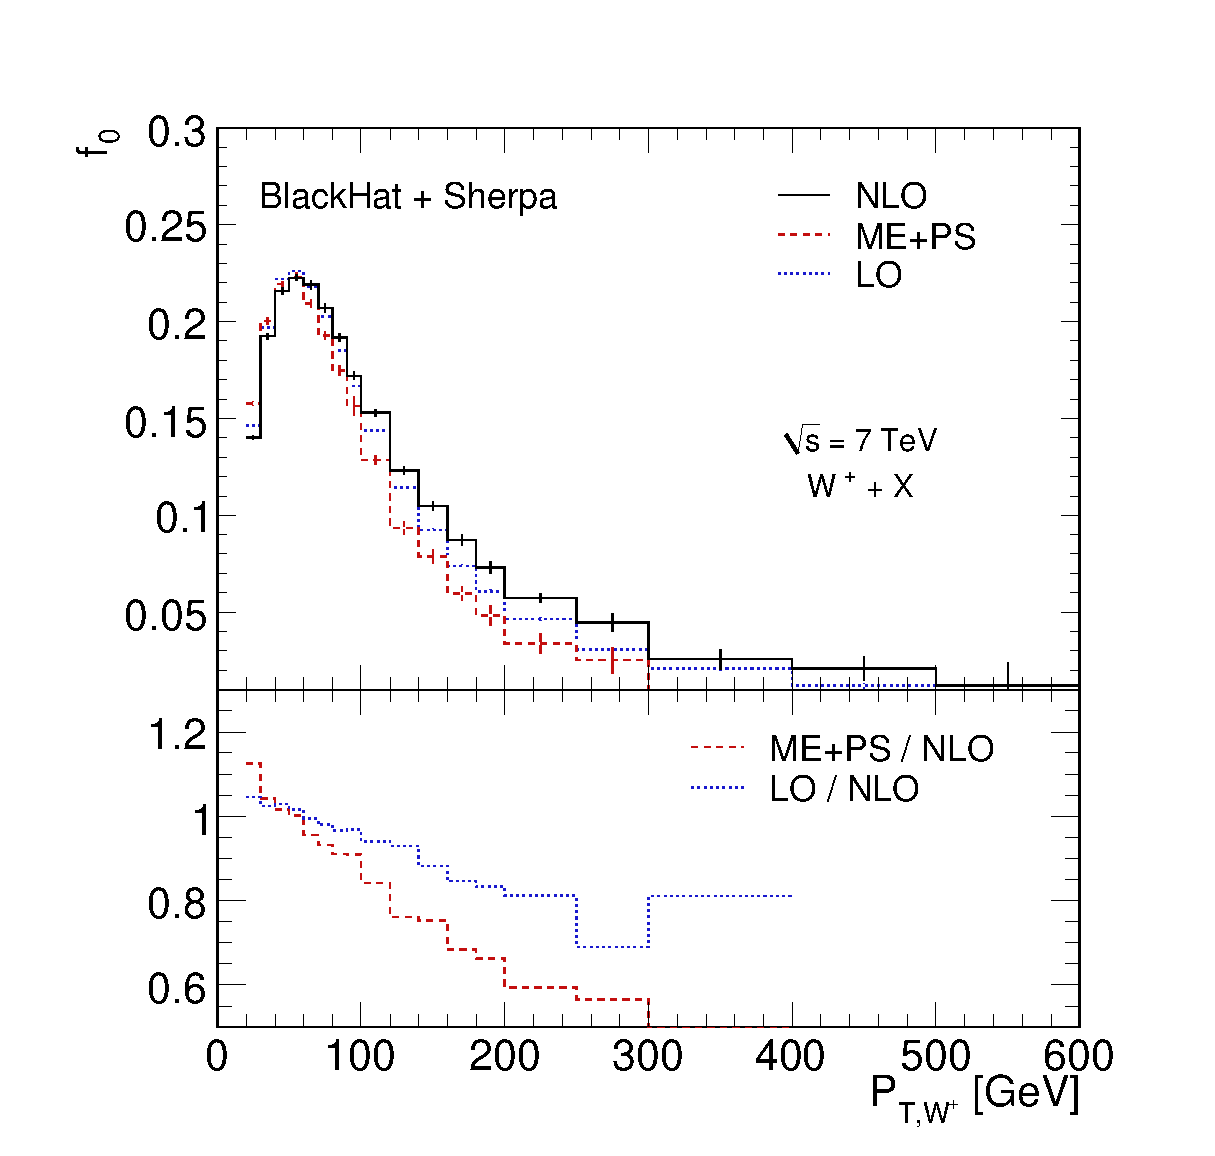
\includegraphics[width=0.29\textwidth]{fig/f0_Wp}}
\caption{The polarisation fractions \fL, \fR and \f0 as a function of \PtW for
  \PWp production are shown in the upper panes of
  \figs~\ref{fig:framework_ptw_fL}, \ref{fig:framework_ptw_fR} and
  \ref{fig:framework_ptw_f0} respectively. Three predictions are shown: the
  fixed-order \ac{NLO} result as a solid black line, the \ac{ME+PS} result as
  red dashed line and the fixed-order \ac{LO} result as a dotted blue
  line. Uncertainties are indicated by thin vertical lines. The lower pane in
  each plot show the ratio of each prediction with respect to the \ac{NLO}
  prediction~\cite{berger_left_handed_w}.}
\label{fig:framework_ptw}
\end{figure}

\section{Modelling New Physics}
\label{sec:framework_susy}
\subsection{\acl{CMSSM}}
\label{sec:cmssm}
It was said in \chap~\ref{sec:susy} that the \ac{MSSM} is problematic from the
point of view of collider searches due to the extremely large number of
parameters associated with \ac{SUSY} breaking. In order to make quantitative
statements about the sensitivity of a given experimental search, a more
restricted theory must be considered.

One such theory that has often been used is the \ac{CMSSM}. The \ac{CMSSM} is
inspired by \ac{mSUGRA}~\cite{kane_minimal}. This proposes a
gravity-mediated \ac{SUSY} breaking mechanism via a hidden sector. This
assumption reduces the parameter space of the \ac{MSSM} to just 5 parameters, 4
of which are continuous:
\begin{itemize}
\item a universal trilinear scalar coupling, $A_0$;
\item a single scalar mass, $m_0$;
\item a single gaugino mass, $m_{\frac{1}{2}}$;
\item $\tan\beta$ where $\beta$ is the ratio of the Higgs' vacuum expectation values and
\item $\textrm{sign}(\mu)$ where $\mu$ is the self-coupling of the Higgs field.
\end{itemize}

Whilst this proves to be a much more practical model from the point of view of
experimental searches, there is no particular reason to assume that \ac{SUSY} is
broken in this way. The restricted parameter space of the \ac{CMSSM} may
disfavour a number of topologies which would appear in a larger class of
\ac{SUSY} theories. An additional, but related difficulty is that
interpretations of results within the \ac{CMSSM} may not be robustly
extrapolated to alternative models. As will be seen, both of these difficulties
are addressed by a more generic set of \ac{SUSY}-inspired models. These will be
presented in the next section.

\subsection{Simplified Models}
\label{sec:sms}
It is often the case that theorists, having devised some theory, and made
concrete phenomenological predictions from it, wish to test it against
experimental data. The difficulty then arises of taking these predictions and
translating them into a form where they can be compared directly with
experimental results. Typically, these results will be provided in the form of
one or more event yields, corresponding background predictions and statistical
and systematic uncertainties. In some (but probably not most) cases, the
relevant correlations will also be included. The theorist must then take the
predictions of the theory and apply experimental resolution effects to them in
order to simulate the expected signal yield. Modern detectors are highly complex
and require very complex simulation to precisely model all of the resolution and
acceptance effects. In some cases, in particular for relatively simple kinematic
quantities, a simplified parameterisation may suffice. However, detailed checks
will be required to confirm that a given approximation reproduces, with adequate
fidelity the results of the full detector simulation or the actual recorded
data. If it can be confirmed that this is the case, the theorist may then
proceed to redo the work of the experimentalist in modelling the various
statistical and systematic effects in the form of a likelihood
function. Finally, they may then utilise all of these components to produce
their own interpretation of the data against the chosen theory.

Clearly, this procedure is both laborious and error-prone. It was therefore
proposed that the \ac{LHC} experiments would provide a richer interpretation in
the context of a set of ``Simplified Models''. Broadly speaking, a simplified
model is an effective theory, chosen to characterise a particular
phenomenological scenario present within one or more \ac{NP} models. Free
parameters which have little effect on the physics (at least at small integrated
luminosities) are integrated out, leaving only those with a greater effect on
the physics. By constructing a number of these models, the full space of
possibly physical signatures arising in much more complicated theories may be
spanned. This collection of models is sometimes referred to as a \acf{SMS}

Although the concept of a simplified model is quite general, the discussion here
will now focus on those inspired by \ac{SUSY} or ``\ac{SUSY}-like'' theories,
and more specifically those giving rise to single lepton final states.

\subsubsection{Dark Matter Models}
As discussed in \chap~\ref{sec:susy}, a highly desirable prediction of certain
supersymmetric theories is the existence of a stable, weakly-interacting
particle or \ac{WIMP}. This is a dark matter candidate with a striking
experimental signature at collider experiments -- a large missing energy
component. Since these topologies are largely inspired by \Rparity conserving
\ac{SUSY}, similar terminology and notation will be used to refer to their
particle content. This should not be taken to suggest that these topologies are
exclusive to \ac{SUSY} type theories.

The topologies considered here may be split into two categories. The first
begins with pair-production of a neutral, coloured object -- the gluino in the
case of \ac{SUSY}. The second is initiated by production of a charged, coloured
object -- the squark of \ac{SUSY} . As for the \ac{CMSSM}, if suitably light,
these are expected to be produced most abundantly at the \ac{LHC}.

In either case, the squark or gluino-type particle then decays, either directly
to an \ac{LSP} or via some intermediate particles (comparable to the heavy
electroweakinos of \ac{SUSY}) -- a cascade decay.
% The naming convention adopted here gives each model a name, T$x$. For models
% resembling pair production of the gluinos, $x$ will be an odd integer and for
% those representing squark production, an even integer. For gluino-type
% topologies, $x$ values of 1, 3 and 5 represent respectively: direct decay of
% both particles, one cascade and one direct decay and two cascade decays. The
% squark-type models are similarly labelled 2, 3 and 4 representing the same
% combinations of direct and cascade decays.

\begin{figure}[h!]
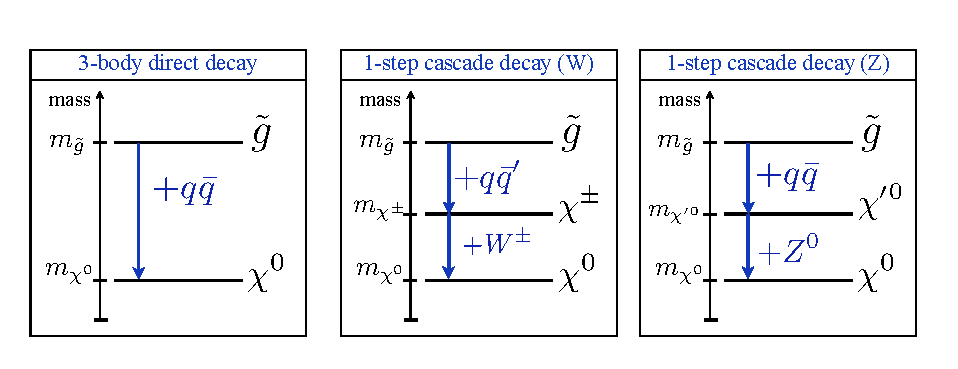
\includegraphics[width=\textwidth]{fig/gluino_sms_decays}
\caption{Illustration of direct and cascade gluino decay modes within \ac{SUSY}
  simplified models.~\cite{alves_simplified_2011}}
\label{fig:gluino_sms_decays}
\end{figure}

\subsubsection{Connection to Supersymmetry}
Considering first the gluino pair-production models
(\fig~\ref{fig:gluino_sms_decays}), we shall assume that the squarks are heavier
and therefore kinematically inaccessible. If this were not the case, the
phenomenology would be better described by the squark-type models.

In such supersymmetric models, the gluino may decay only via an off-shell
squark~\cite{alwall_simplified}. This may be either directly to the LSP or
indirectly via intermediate states. Direct decays correspond to \ac{SUSY}
scenarios where either~\cite{alves_simplified_2011}:
\begin{itemize}
\item $\PSgxzi \approx \PSB$ and the $\PSq_{R}$ are lightest or the $\PSW$ is kinematically
  inaccessible;
\item $\PSgxzi \approx \PSW$ and either $\PSq_{L}$ are lightest or there is no
  splitting between the left and right-handed squarks and
\item $\PSgxzi \approx \PSH$ and either heavy-flavour squarks are inaccessible or
  $\PSB$ and $\PSW$ are inaccessible.
\end{itemize}

This is not generally true in either \ac{mSUGRA} or \ac{GMSB} but does
correspond to certain \ac{AMSB} scenarios~\cite{alves_simplified_2011}.

Alternatively, the gluino may undergo a cascade decay via an intermediate mass
state, either a chargino or a heavy neutralino. This will subsequently decay to
the \ac{LSP} via either a $\PW$ or $\PZ$ boson.

The situation is similar in the case of squark pair-production, except that
without the intermediate off-shell squark, the jet multiplicity is reduced.

\subsubsection{Single Lepton Topologies}
To provide a meaningful interpretation of the single lepton search detailed in
\chap~\ref{sec:susysearch}, two simplified models have been chosen. The models,
\TthreeW and \Ttwott, have been chosen in particular since they offer topologies
which are likely to enter the selection of a single lepton \ac{SUSY} search.

\begin{figure}[h!]
\centering
\subfloat[]{\label{fig:sms_topologies_t3w}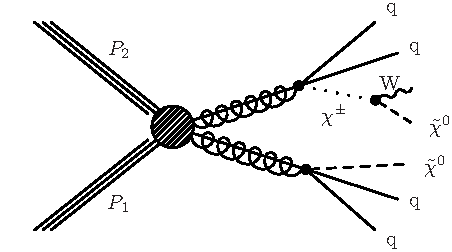
\includegraphics[width=0.45\textwidth]{fig/T3w}}\quad
\subfloat[]{\label{fig:sms_topologies_t2tt}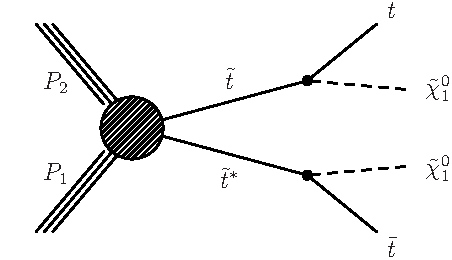
\includegraphics[width=0.45\textwidth]{fig/T2tt}}
\caption[Illustration of two simplified model topologies suited to a single
lepton supersymmetry search]{Illustration of two simplified model topologies
  suited to a single lepton supersymmetry search:
  \subref{fig:sms_topologies_t3w} \TthreeW and \subref{fig:sms_topologies_t2tt}
  \Ttwott~\cite{susy_interpretation_pas}}
\label{fig:sms_topologies}
\end{figure}

The \TthreeW model is a gluino pair-production model, in which one of the mother
particles undergoes a cascade decay via an intermediate particle. The $\PW$ in
the model name indicates that this intermediate particle is then ``forced'' to
decay to a \PW boson. This topology is illustrated in
\fig~\ref{fig:sms_topologies_t3w} and is seen to be similar to the example
\ac{SUSY} decay illustrated in \fig~\ref{fig:susy_1lep_decay}. This model is
parameterised by the mass of the mother particle, \Mgluino, the mass of the
daughter particle, \Mlsp and the mass of the intermediate particle, \Mchargino.

The second model, \Ttwott, begins with squark pair production. Both mother
particles decay directly to the \ac{LSP}. Furthermore, both squarks are assumed
to be stop particles -- the superpartner of the top quark -- each decaying to a
\ac{SM} top quark. This decay topology is illustrated in
\fig~\ref{fig:sms_topologies_t2tt}. Such events with two top quarks in the final
state, should give an experimental signature suitable for a single lepton
search.

The \Ttwott model reflects scenarios in which the stop is the lightest of the
squarks. These are theoretically attractive for a number of reasons
(see~\cite[{p.~202}]{sparticles} and~\cite{light_stop}). Since this does not
contain an intermediate mass state, it has only two paramters: the mass of the
mother, \Mstop and the mass of the daughter, \Mlsp.

\subsubsection{Combining Topologies}
For phenomenological purposes, each separate decay topology may be considered as
an independent simplified model. The predictions of a whole set of topologies
can then be combined by taking linear combinations. For direct comparison
against experimental data, it is desirable to simulate a desired set of
topologies within a monte-carlo generator by ``turning on'' the chosen physics
subprocesses. The model parameter space can be sampled by moving through a
lattice of values in the desired range. At each lattice site, a statistically
sufficient number of events is generated with the appropriate parameter values
inserted into the configuratxoion of the \ac{MC} generator.
  \chapter{The \acl{CMS} Experiment at the \acl{LHC}}
\label{sec:experiment}
\section{Introduction}
The \acf{LHC}~\cite{lhc_design_report} is a proton-proton ($\Pp\Pp$) accelerator
located at the CERN particle physics laboratory near Geneva, Switzerland. It has
been designed to carry out a broad program of physics research using a number of
specialised detectors. This chapter will give a very brief introduction to the
\ac{LHC} itself. The \acf{CMS} experiment, a large, general purpose detector at
the \ac{LHC}, will be discussed in detail.

\section{The \acl{LHC}}
The \ac{LHC} is a circular synchrotron, \unit{27}{\kilo\metre} in circumference,
sitting on the border between France and Switzerland. It has been built in a
tunnel initially constructed to house the \ac{LEP} accelerator, buried at a
depth of between 50 and \unit{175}{\metre} underground. Although primarily a
$\Pp\Pp$ accelerator, the \ac{LHC} will also undertake a heavy-ion physics
program. At full design specifications, 2808 bunches of protons will circulate
around each direction of the ring, colliding at a centre-of-mass energy of
\unit{14}{\TeV}. It is designed to eventually reach a proton bunch spacing of
\unit{25}{\ns} and an instantaneous luminosity of
\unit{$10^{34}$}{\rpsquare{\centi\metre}\usk\reciprocal\second}.

There are four primary experiments at the \ac{LHC}:
\ac{ALICE}~\cite{alice_proposal}, \ac{ATLAS}~\cite{atlas_proposal},
\ac{CMS}~\cite{cms_technical_proposal,cms_jinst} and the
\ac{LHCb}~\cite{lhcb_proposal} experiment. Each one is constructed around one of
the four interaction points and records the shower of particles produced from
the colliding protons. \ac{ATLAS} and \ac{CMS} are large, general purpose
detectors, designed to search for a variety of \ac{NP} signatures as well as
making higher precision measurements of many \ac{SM} parameters. \ac{ALICE} is
optimised to examine the products of heavy-ion collisions (principally lead-lead
-- although a number of configurations are possible) in order to explore the
quark-gluon plasma and related physics. Finally, the \ac{LHCb} experiment is
optimised for the study of B-meson decays. These are important for exploring
CP violation within the \ac{SM} but might also provide potential avenues for the
discovery of \ac{NP}.

In addition to the four larger detectors, two smaller experiments lie upstream
of the \ac{ATLAS} and \ac{CMS} collision points in order to probe more
specialised forward physics phenomena. These are the
\ac{LHCf}~\cite{lhcf_proposal} and \ac{TOTEM}~\cite{totem_proposal} experiments.

\subsection{Accelerator Complex}
The \ac{LHC} ring itself is the final stage in an injector chain which
incorporates a series of accelerators built at CERN over the last 50 years. It
is illustrated in \fig~\ref{fig:expt_lhc}. Each stage supplies an incremental
increase in the proton (or heavy ion) bunch energy. The first stage in this
chain is a linear accelerator -- either the Linac2 for proton injection or
Linac3 during heavy-ion runs. The Linac2 injects protons into the \ac{PSB} at an
energy of \unit{50}{\mega\electronvolt}. Similarly, the ions proceed first from
the Linac3 to the \ac{LEIR} before finally arriving at the \ac{PS}. From here
on, the paths of the protons and heavy-ions are the same. Proton bunches pass
from the \ac{PSB} to the \ac{PS} at an energy of \unit{1.4}{\giga\electronvolt}
and then on to the \ac{SPS} at an energy of
\unit{26}{\giga\electronvolt}. Having arrived at the \ac{SPS}, the protons
circulate around a ring \unit{2}{\kilo\metre} in diameter, where their energy is
increased to \unit{450}{\giga\electronvolt}. From here, kicker magnets inject
the bunches into the \ac{LHC} itself, where the energy can finally be increased
to the design-specified \unit{7}{\TeV} per proton beam. The 2010 and 2011
data-taking periods were at \unit{3.5}{\TeV} per proton beam, with an increase
to \unit{4}{\TeV} planned for 2012.

\begin{figure}[h!]
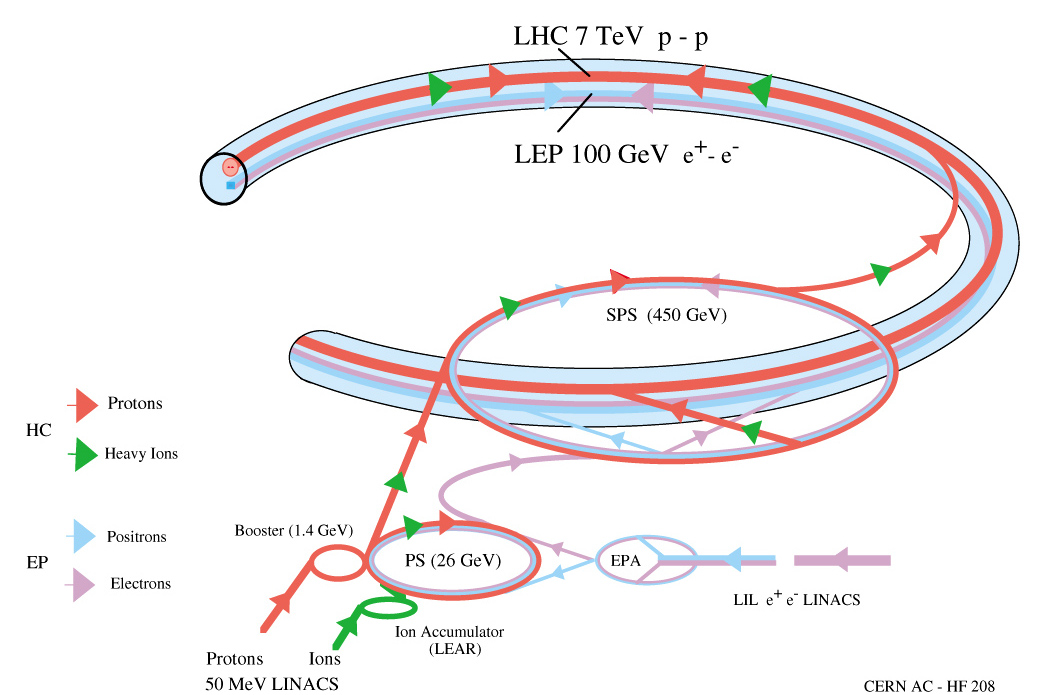
\includegraphics[width=0.8\textwidth]{fig/lhc-pho-1993-008_cropped}
\caption[Illustration of the \acs{LHC} accelerator complex]{Illustration of the
  \ac{LHC} accelerator complex showing the path of protons and heavy-ions
  through a series of accelerators at \ac{CERN}~\cite{lhc_injection}.}
\label{fig:expt_lhc}
\end{figure}

\section{The \acl{CMS} Experiment}
\label{sec:cms}
\ac{CMS} is a large, general purpose detector~\cite{cms_jinst} at the
\ac{LHC}. It has been designed to search for the Higgs boson (see
\sec~\ref{sec:sm_higgs}) as well as signatures of physics beyond the \ac{SM}.

The design goals of CMS were as follows (paraphrasing the technical proposal
document~\cite{cms_technical_proposal}):
\begin{enumerate}
\item a high quality, redundant muon system,
\item the best possible \ac{ECAL}
\item high quality central tracking to complement these two systems and
\item an affordable detector.
\end{enumerate}

\begin{figure}[h!]
\centering
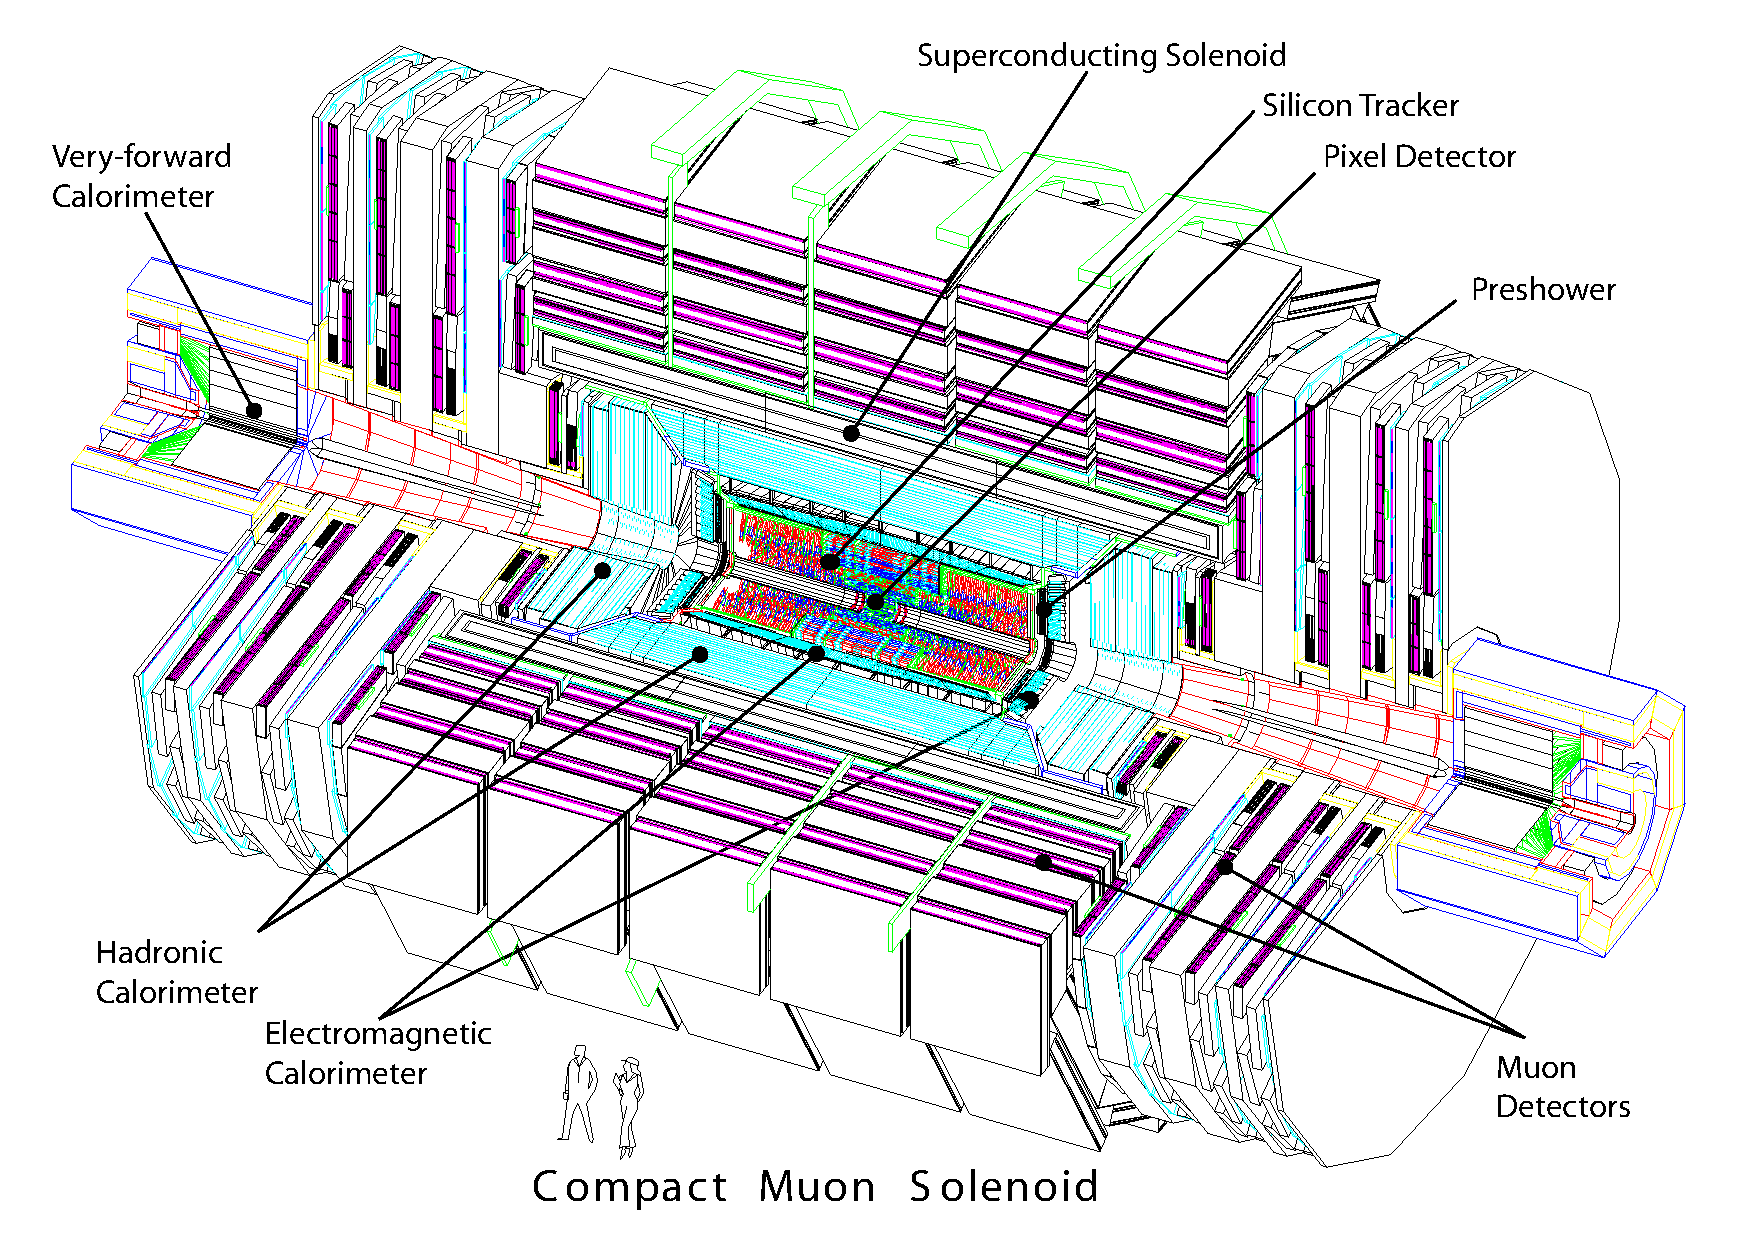
\includegraphics[width=0.7\textwidth]{fig/cms_complete_labelled}
\caption[Illustration of the \acs{CMS} detector]{Illustration of the \ac{CMS}
  detector with subdetectors labelled~\cite{cms_jinst}.}
\label{fig:expt_cms}
\end{figure}

\ac{CMS} adopts a traditional cylindrical design (see
\fig~\ref{fig:expt_cms}), \unit{21.5}{\metre} in length and
\unit{15}{\metre} in diameter. A key feature of the detector is the
superconducting solenoid, delivering a nominal \unit{4}{\tesla}
magnetic field. The bending field supplied provides accurate muon
momentum resolution up to energies of \unit{$\approx$ 1}{\TeV}. The
size of the solenoid placed stringent limitations on the volume of the
inner detector subsystems (everything except for the muon chambers and
return yoke).

\subsection{Coordinate System}
The coordinate system at \ac{CMS} is right-handed, with its origin placed at the
nominal beam collision point inside \ac{CMS}. The $x$ axis is then defined to
point horizontally inwards towards the centre of the \ac{LHC} ring and the
$y$-axis, vertically upwards. The $z$-axis is aligned along the beam-line,
pointing towards the nearby Jura mountains. Often a cylindrical coordinate
system will be used where the azimuthal angle, $\phi$, and radial
coordinate, $r$, span the $x-y$ plane. The azimuthal angle is measured with
respect to the $x$-axis. The pseudorapidity, $\eta = - \ln \tan
\frac{\theta}{2}$ where $\theta$ is the polar angle measured with respect to the
$z$-axis.

\subsection{Silicon Tracker}
The innermost subsystem of \ac{CMS} is the silicon tracker~\cite{tracker_paper},
designed to provide highly precise measurements of particle trajectories close
to the CMS interaction point. It is shown in cross section in
\fig~\ref{fig:expt_tracker}. The tracker extends to pseudorapidities of
$|\eta|<2.5$ and has an active silicon area of more than
\unit{200}{\metre\squared}, making it the largest silicon tracker ever built.

\begin{figure}[h!]
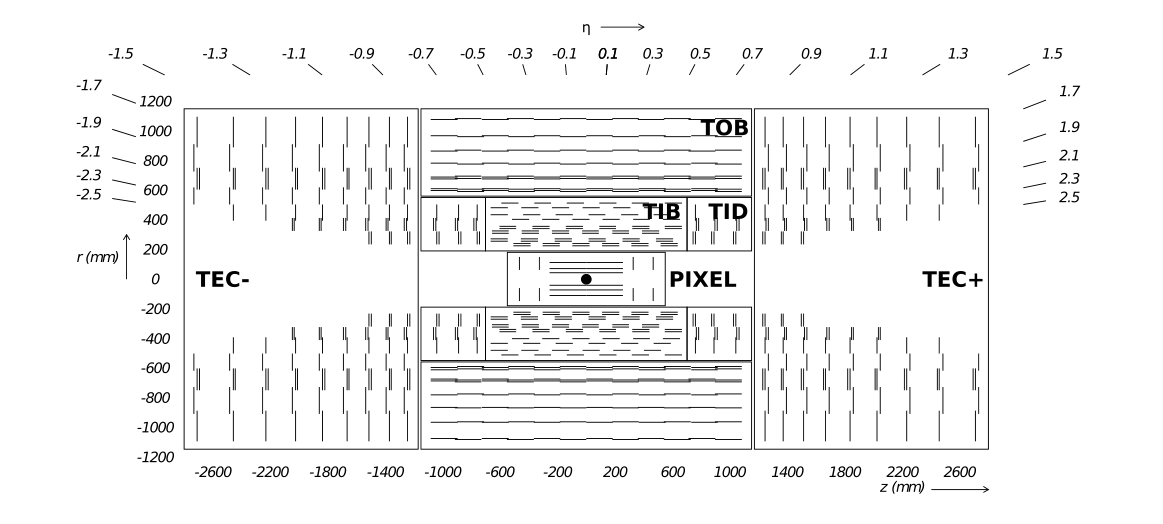
\includegraphics[width=\textwidth]{fig/tracker2}
\caption[Schematic cross section through the CMS tracker]{Schematic cross
  section through the CMS tracker. Each line represents a detector
  module. Double lines indicate back-to-back modules which deliver stereo
  hits~\cite{cms_jinst}.}
\label{fig:expt_tracker}
\end{figure}

The tracker design can be better understood by considering the expected particle
flux at design luminosity as a function of radial distance, $r$, from the
beam-line.
\begin{itemize}
\item At $ r \approx \unit{10}{\cm}$ the particle flux is highest. Accordingly,
  the innermost layer of the CMS tracker is comprised of hybrid pixels. With an
  area of \unit{$100\times 150$}{\micro\metre\squared}, particle densities are
  $O(10^{-4})$ per pixel per LHC bunch crossing.
\item At a radius \unit{$20 < r < 55$}{\centi\metre}, reduced particle flux allows
  the use of silicon microstrip sensors. With a much larger area of
  $\unit{10}{\centi\metre}\times\unit{80}{\micro\metre}$, average particle
  densities are $O(10^{-2})$ per strip per bunch crossing.
\item At $ r > \unit{55}{\cm}$, still larger silicon strips can be used, with
  sizes up to $\unit{25}{\cm}\times\unit{180}{\micro\metre}$. This gives a
  particle density of $O(10^{-2})$ per strip per bunch crossing.
\end{itemize}

\subsubsection{Pixel Tracker}
The hybrid pixels are placed closest to the interaction point. As well as
maintaining an acceptable particle density per sensor, their close proximity to
the interaction point allows the origin of collision products to be accurately
determined. In the barrel region, 3 layers are placed at mean radii of 4.4, 7.3
and \unit{10.2}{\cm}. The detector has a length of \unit{53}{\cm} in the $z$
direction. The end discs are instrumented with only two layers and are located
at $|z|=34.5, \unit{46.5}{\cm}$. The pixel modules in these layers are arranged
in a ``turbine-like'' layout.

\subsubsection{Strip Tracker}
Further from the interaction point, the tracker is instrumented with silicon
strip detectors. The barrel component can be further divided into the \ac{TIB}
and the \ac{TOB}. The \ac{TIB} is composed of 4 layers and the \ac{TOB} a
further 6. The \ac{TOB} extends to $z = \pm \unit{118}{\centi\metre}$. Beyond
this are the endcaps which can again be split into two components: the \ac{TEC}
made up of 9 disks and the \ac{TID}, 3. The silicon micro-strip sensors are
\unit{320}{\micro\metre} thick and oriented parallel to the $z$-axis in the
barrel and radially in the disks.

Both the \ac{TIB} and \ac{TID} supply up to four measurements in $r-\phi$. The
inner two layers of the \ac{TIB} have a strip-pitch of \unit{80}{\micro\metre},
and the outer two, \unit{120}{\micro\metre}. These achieve single point
resolutions of \unit{23 and 35}{\micro\metre} respectively. In the \ac{TID}, the
strip pitch varies between \unit{100 and 141}{\micro\metre}.

The \ac{TOB} uses \unit{500}{\micro\metre} thick sensors with a strip-pitch of
\unit{183}{\micro\metre} in the first four layers and \unit{122}{\micro\metre} in
the outer two. This gives a single point resolution of \unit{53}{\micro\metre}
and \unit{35}{\micro\metre} respectively.

The first two layers of the \ac{TIB}, \ac{TOB} and \ac{TID} and rings 1, 2 and 5
of the \ac{TEC} are so-called ``stereo modules''. These are double-sided modules
where the two layers of strips have a stereo angle of \unit{100}{\milli\radian}
between them. This provides additional resolution in the $z$ measurement in the
barrel (or $r$ in the endcaps). The resolution of this measurement is
\unit{230}{\micro\metre} and \unit{530}{\micro\metre} in the \ac{TIB} and
\ac{TOB} respectively.

\subsection{\acl{ECAL}}
The \ac{ECAL} surrounds the silicon tracker and provides a high resolution
measurement of electromagnetic showers within a homogeneous, hermetic
calorimeter~\cite{ecal_paper}. The barrel region alone comprises 61,200 lead
tungstate (PbWO$_4$) crystals, with 7,324 in each of the two endcaps. This
material was chosen for its high density, short radiation length and small
Moli\`{e}re radius. Scintillation photons are then recorded by \acp{APD} in the
barrel and \acp{VPT} in the endcap. The driving motivation for the \ac{ECAL}
design was the detection of the low-mass favoured Higgs decay channel
$\PH\longrightarrow\gamma\gamma$.

\subsubsection{\acl{EB}}
The \ac{EB} extends in rapidity to $|\eta|<1.479$ with a crystal segmentation
of $360\times 85$ in $\eta-\phi$ for each half-barrel. Each crystal is slightly
tapered, with a cross-section of $0.0174\times0.0174$ in $\eta-\phi$. The
crystals have a front cross section of \unit{$22\times
  22$}{\milli\metre\squared} and a length of \unit{230}{\milli\metre}
(corresponding to 25.8 radiation lengths).

\subsubsection{\acl{EE}}
The \ac{EE} occupies the rapidity range $1.479 < |\eta| < 3.0$. Crystals are
grouped into $5\times 5$ ``supercrystals'' within a carbon-fibre alveolar
structure. The endcaps are split into two halves, known as ``Dees'', each
holding 3,662 crystals.

The scintillation of the \ac{ECAL} crystals as well as the amplification of the
\acp{APD} varies as a function of temperature. This variation was found to be
\unit{$\approx 4\%$}{\per\celsius}. For this reason, the \ac{ECAL} temperature
is precisely regulated to within \unit{$\pm$ 0.05}{\celsius}.

\subsubsection{\ac{ECAL} Transparency and the \ac{CMS} Laser Monitoring System}
\label{sec:expt_laser_monitoring}
The PbWO$_4$ crystals that make up the \ac{ECAL} are radiation resistant but
quickly suffer a decrease in their optical transmission under
irradiation~\cite{ecal_transparency}. This is a result of the formation of
colour centres which absorb a fraction of the incident light. At a working
temperature of \unit{18}{\celsius}, the damage anneals leading to an equilibrium
in the optical transmission properties which are constant with dose rate. The
consequence of this is a cyclic change in the optical transmittivity of the
crystals as the \ac{LHC} moves between colliding beams and machine
refills. Since this depends on dose rate, the effect is a function of \ac{LHC}
luminosity and rapidity. It is expected to range from a shift of $\sim 2\%$ in
the barrel at low luminosity to $> 10\%$ in the endcaps at high luminosity. The
magnitude of this effect on energy and momentum measurements would be disastrous
if not properly accounted for. Correction for this effect necessitates constant
monitoring of the transparency -- a task performed by the laser monitoring
subsystem~\cite{laser_monitoring}.

Three lasers are used for the transparency measurement: two blue ($\lambda
\approx \unit{440}{\nano\metre}$) and one near-infrared ($\lambda \approx
\unit{796}{\nano\metre}$). The blue laser (with a second fitted for redundancy
purposes) is close to the scintillation emission peak and thus can be used to
track the changes in the crystal transparency. The near-infrared laser is far
from the emission peak and thus relatively stable to changes in the
transparency. This can be used to verify the stability of the system. The lasers
are distributed to the crystals via optical fibres and a series of
fan-outs. Approximately 1\% of the \ac{LHC} beam gap of
\unit{3.17}{\micro\second} is used for transparency monitoring. A full scan of
the entire \ac{ECAL} can be achieved in approximately 30~minutes. The lasers can
be pulsed at $\approx \unit{80}{\mega\hertz}$ with a pulse timing jitter of
\unit{3}{\nano\second}. This is adequate for synchronisation with the \ac{LHC}
bunch crossings.

The transparency of the crystals is derived from the response of the \ac{APD}
normalised to the height of the laser pulse, as measured using a silicon
photodiode. Due to differences in path length and optical spectra between the
laser and the scintillation light, the transparency of the crystals may be
related to the measured transparency via a power law.

\subsection{\acl{HCAL}}
Accurate measurement of hadronic showers is crucial for analyses involving jets
or missing energy signatures. The \ac{HCAL}~\cite{hcal_paper} lies between the
outer edge of the ECAL and the inner edge of the solenoid ($\unit{1.77}{\metre}
< r < \unit{2.95}{\metre}$). This constrains the size of the \ac{HCAL} to a
relatively compact design and necessitates the placement of a ``tail catcher''
outside of the solenoid.

\subsubsection{\acl{HB}}
The \ac{HB} comprises 36 azimuthal wedges, with 18 in each half barrel. Each
wedge consists of alternating layers of brass absorber plates and plastic
scintillators. The light from these plates is then carried via
wavelength-shifting fibres to a \ac{HPD} for readout. The number of interaction
lengths increases with polar angle, from 5.82 at $90\degrees$ to 10.6 at
$|\eta|=1.3$~\cite{hcal_design}.

\subsubsection{\acl{HE}}
The \ac{HE} covers the rapidity range $1.3 < |\eta| < 3$ and receives a larger
radiation flux than the \ac{HB}. Each endcap consists of 36 wedges, and
wavelength shifting fibres are once again used to take light from plastic
scintillators to \acp{HPD}. Including the \ac{ECAL}, the \ac{HE} depth is
equivalent to $\approx 10$ interaction lengths.

\subsubsection{\acl{HO}}
The \ac{HO} or ``tail catcher'' provides increased sampling depth in the
rapidity region $|\eta| < 1.3$ where the \ac{HB} and \ac{EB} do not provide
sufficient containment. Since the \ac{HO} lies outside the solenoid, its design
is constrained by that of the muon chambers -- with 5 rings in $\eta$. The
solenoid coil provides additional absorption, giving the calorimeter system a
minimum depth of 11.6 interaction lengths.

\subsubsection{\acl{HF}}
The \ac{HF} is positioned in the rapidity range $|\eta|>3$ and consequently must
endure a much larger particle flux -- approximately \unit{760}{\GeV} per
proton-proton interaction (versus $\approx \unit{100}{\GeV}$ for the rest of the
detector). Radiation hardness was thus a leading consideration in its design.

Quartz fibres are interleaved between steel absorbers. Shower particles above
the Cherenkov threshold ($E \geq \unit{190}{\keV}$ for electrons) produce
Cherenkov light. This is routed to the rear of the calorimeter and read out by
\acp{PMT}. The \ac{HF} is most sensitive to the electromagnetic component of the
shower.

\subsection{Muon Chambers}
Accurate measurement of muons is one of \ac{CMS}' key design goals. The effect
of radiative losses in the tracker is much less for muons than it is for
electrons. Thus muons are able to provide a much finer mass resolution at low
transverse momentum. This is an important advantage for a variety of physics
searches and measurements at \ac{CMS}. The muon system is responsible for muon
identification, momentum measurement and triggering (for further detail see
\sec~\ref{sec:trigger}). Three types of detectors are used, chosen for different
regions of the detector according to the magnetic field, muon rate and response
time required for input to the trigger.

\subsubsection{\aclp{DT}}
In the barrel region, the magnetic field is relatively uniform and the muon flux
low enough to allow the use of the \acf{DT}~\cite{dt_paper}. These identify
muons in the region $|\eta| < 1.2$. The drift chamber was first developed as a
refinement of earlier wire proportional chamber designs in which the drift time
of the electrons to the anode wire is used to provide additional spatial
resolution. This allows the wire spacing to be increased, thus reducing the
electronics requirements.

Each \ac{DT} is composed of 2 (or 3) ``super-layers'', with each super-layer
further divided into 4 layers of rectangular drift cells. Of the four concentric
muon stations in the barrel, the inner three contain 60 drift chambers and the
outermost, 70. The wires in the outer two layers of each drift cell are oriented
parallel to the beam line, providing a measurement in the $r\phi$ direction (in the
magnetic bending plane). The inner two layers are perpendicularly aligned,
giving a measurement of the $z$ coordinate.

\subsubsection{\aclp{CSC}}
In the endcap region, the large muon and background rate coupled with the
strong, non-uniform magnetic field, prevent the use of \acp{DT}. Instead, an
alternative instrument is used -- the \ac{CSC}~\cite{csc_paper}. The CMS muon
system endcap consists of 468 \acp{CSC}, each a trapezoidal multiwire
proportional chamber arranged radially covering an azimuthal angle $\Delta\phi$
of either 10 or 20 degrees. Each \ac{CSC} has 6 anode wire planes interleaved with 7 cathode strip planes. The wire
readout provides a measurement of the $r$ coordinate whilst a measurement of
$\phi$ is obtained by interpolating charges on the cathode strips.

\subsubsection{\aclp{RPC}}
The trigger (see \sec~\ref{sec:trigger}) requires a muon detector capable of
providing a fast signal with adequate spatial resolution. This is the
\acf{RPC}~\cite{rpc_paper}, a gaseous, parallel-plate detector with spatial
resolution suitable for both barrel and endcap regions and a response time much
less than the \unit{25}{\nano\second} between consecutive \ac{LHC}
bunch-crossings. This allows the \ac{RPC} to unambiguously identify the
bunch-crossing assignment for a muon track, even in the presence of the large
backgrounds and high rates of the \ac{LHC} environment.

\subsection{Data Acquisition and Trigger System}
\label{sec:trigger}
The high luminosity of the \ac{LHC} beam leads to a high particle flux in the
detector. The separation of particles in the detector becomes increasingly
difficult. In addition, many analyses benefit from precise position and momentum
measurements. Consequently, the \ac{CMS} subdetectors are constructed with an
extremely fine granularity. Unavoidably, this requires an extremely large number
of read-out channels - approximately 55 million across the whole detector. To
make matters worse, the \ac{LHC} is planned to achieve a bunch-spacing of only
\unit{25}{\nano\second}. For these reasons, the \ac{DAQ} system at \ac{CMS}
faces the simultaneous challenges of large bandwidth and low-latency.

Tightly coupled to the \ac{DAQ} is the trigger system~\cite{tridas}. The huge
number of readout channels in \ac{CMS} is not only a challenge in terms of the
bandwidth of the \ac{DAQ} but also poses serious difficulties relating to
long-term storage requirements. A digitised, zero-suppressed event dump from
\ac{CMS} is approximately \unit{2}{\mega\byte} in size. With an event rate of up
to \unit{40}{\mega\hertz}, this would require a storage rate of
\unit{80}{\tera\byte\per\second}. Despite the rapid improvement in disk storage
technology over the last few decades, such storage capacities are clearly
infeasible both in terms of capacity and \ac{IO} requirements. For these
reasons, a system capable of quickly rejecting a very large fraction of
collisions is required. This is known as the trigger.

\subsubsection{Triggering at \ac{CMS}}
The trigger at \ac{CMS} is split into two stages. The first stage, the \ac{L1T},
must operate at the full \ac{LHC} bunch-crossing frequency. To achieve adequate
latency, it is implemented almost entirely within electronic logic -- either
\acp{FPGA} or custom designed integrated circuits. The \ac{L1T} must reduce the
rate to \unit{100}{\kilo\hertz}.

In the second stage of the trigger, the \ac{HLT}, the rate is further reduced to
$O(\unit{100}{\hertz})$. Due to the reduced rate, the \ac{HLT} is implemented in
software running in a computing farm. Since the \ac{HLT} has access to a full
read-out of the detector, and more time to issue a trigger decision, more
sophisticated trigger algorithms are used. Often these are similar to those used
by the off-line reconstruction.

\subsubsection{The \acl{L1T}}
\label{sec:l1t}
The \ac{L1T} must produce a trigger decision with minimal latency. This latency
is chiefly limited by the size of the pipeline on the \ac{APV25} chip used to
readout from the silicon strip tracker. The \ac{APV25} samples the voltage from
the silicon strips at \unit{25}{\nano\second} intervals. These are stored in a
pipeline, 192 samples deep. This constrains the \ac{L1T} to provide a decision
within $\approx \unit{3.2}{\micro\second}$.

The \ac{L1T} has limited access to detector subsystems and only a limited time
in which to issue a trigger decision. In particular, since tracker measurements
are not available, distinction between electrons and photons is not
possible. The challenge for the \ac{L1T} is therefore not only to make a fast
decision using limited information from the detector, but also to ensure that
potentially interesting events are retained and passed onto the \ac{HLT} for
more thorough analysis.

\begin{figure}[h!]
\centering
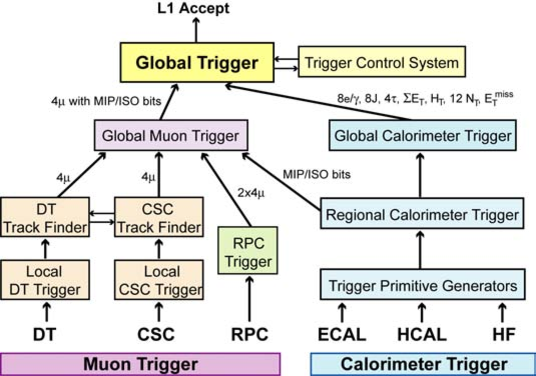
\includegraphics[width=0.7\textwidth]{fig/trigger}
\caption[Diagram showing the organisation of the \acs{CMS} \acs{L1T}]{Diagram
  showing the organisation of subsystems within the \ac{CMS} \ac{L1T}.}
\label{fig:expt_cms_trigger}
\end{figure}

The structure of the \ac{L1T} is shown in \fig~\ref{fig:expt_cms_trigger}. The
\ac{GT} is the final stage in the trigger chain. It receives ``trigger objects''
from two subsystems: the \ac{GCT} and \ac{GMT}. Objects, ranked according to
their energy and quality, are received along with their coordinates in $\eta$
and $\phi$. These objects are processed by 128 algorithms, each of which
produces a trigger decision. The final output of the \ac{GT} is then determined
by a configurable mask, which may be altered to meet different data-taking
objectives. The final trigger decision is then sent to the Timing, Trigger and
Control subsystem in order to initiate a read-out of the detector.

The calorimeter trigger subsystem begins with the \ac{TPG}. This sums energy
deposits from the \ac{ECAL} and \ac{HCAL} into ``trigger towers''. These are
received by the \ac{RCT}, where electron/photon candidates are found and the
trigger tower energies summed into larger ``\ac{RCT} regions''. These consist
of $4\times 4$ trigger towers (except in the \ac{HF} where only a single trigger
tower is included). The \ac{RCT} also records a ``tau-veto'' bit, used to
distinguish jets from hadronic tau decays.

The output of the \ac{RCT} is then processed by the
\ac{GCT}~\cite{jj_thesis}. The \ac{GCT} logic is implemented primarily in
\acp{FPGA}. The \ac{GCT} performs a number of tasks in parallel. It sorts the
list of electron/photon candidates and passes the four highest ranked objects to
the \ac{GT}. It also performs a simple jet-finding algorithm on the \ac{RCT}
regions, classifying them as \emph{forward}, \emph{central} and \emph{tau}
jets. The last category includes jets for which none of the constituent \ac{RCT}
regions has its tau-veto bit set. The four highest ranked of each category are
then forwarded to the \ac{GT}.

The final task of the \ac{GCT} is to form global energy sums. These are the
total transverse energy, missing transverse energy, jet counts and \HT (the
scalar sum of the jet energies). These too are forwarded to the \ac{GT}.

The muon trigger receives input from all three muon subdetectors: \acp{RPC},
\acp{CSC} and \acp{DT}. These are integrated in the \ac{GMT}. The muons received
from each subdetector are matched and sorted by transverse momentum and
quality. The four highest rank candidates are forwarded to the \ac{GT}.

\subsection{Computing at \acs{CMS}}
\label{sec:cms_computing}
To meet the extremely large computation and storage requirements of data analysis
at the \ac{LHC}, analysis tasks are performed using a dedicated computing
grid~\cite{lhc_grid}. Events are first sent to the ``tier-0'' storage site at
\ac{CERN} with additional copies forwarded to a number of ``tier-1'' sites
around the world. Data is made available for analysis use, in various
re-processed forms, at ``tier-2'' and ``tier-3'' grid sites. User analysis jobs
are submitted to the grid, and routed automatically to a suitable site.

Events recorded by the \ac{CMS} detector pass through a chain of reconstruction
stages. At each stage, higher-level physics objects are built out of simpler
ones, with a consequent reduction in the data size. \ac{MC} events are processed
using either a detailed \geantfour simulation~\cite{geant_paper}, or a faster,
parameterised model of the response known as \fastsim. This simulates the
response of the \ac{CMS} subdetectors to the generated particles. After the
detector response has been simulated, \ac{MC} is processed in exactly the same
manner as data.

  \chapter{Physics Objects}
\label{sec:reco}
\section{Introduction}
In the previous chapter, details of the \ac{CMS} detector were presented. We
shall now begin to discuss the algorithms used to reconstruct analysis level
objects and quantities which will be of fundamental importance in later
chapters. The objects of primary interest for these purposes are leptons, jets
and missing energy. The offline reconstruction algorithms used to reconstruct
each object will be presented, along with issues and properties related to data
analysis. Some details of the reconstruction performance at \ac{CMS} will also
be shown. Finally, the \acf{PF} algorithm, which provides a global
reconstruction of the event, will be explained in some detail. As will be seen,
\ac{PF} combines tracking and calorimeter measurements to provide excellent
reconstruction of jets and missing energy.

\section{Leptons}
The reconstruction of charged leptons at \ac{CMS} will now be described. Since
tau leptons are not used by either of the analyses presented in this work, their
reconstruction will not be described here. The interested reader is directed to
relevant literature~\cite{cms_pf_tau_id,tau_reco_cms}.

\subsection{Muons}
\label{sec:reco_muons}
The full details of muon reconstruction at CMS are presented
in~\cite{cms_mu_reco,cms_mu_pas}. A brief overview will be presented here,
focussing on the aspects pertinent to the following analysis chapters. Muons are
reconstructed in both the muon chambers and the silicon tracker. To match this
redundancy in the measurement, a number of reconstruction algorithms are
available.

\subsubsection{Tracker Muons}
Tracker muons begin as tracks in the silicon tracker. All tracks with a $\Pt >
\unit{0.5}{\GeV}$ and $p > \unit{2.5}{\GeV}$ are considered as muon candidates
and extrapolated to the muon stations, accounting for expected energy loss and
multiple scattering effects. If at least one muon track segment matches the
extrapolated tracker track, a tracker muon is reconstructed. This algorithm is
more efficient at low momentum ($p < \unit{5}{\GeV}$) since it requires only a
single segment in the muon chambers.

\subsubsection{Standalone Muons}
Standalone muons are based solely on measurements in the muon chambers. The hits
in each chamber are fit individually to obtain seeds - a position and direction
vector along with an estimate of the transverse momentum. These form the basis
of a track fit in the muon chambers based on the Kalman-filter technique. The
fit is constrained to the vertex in order to reject cosmic ray muons. Since much
of the calibration and validation work for the muon system was performed using
cosmic rays, a separate algorithm was developed for this purpose~\cite{cms_mu_reco_cosmic}.

\subsubsection{Global Muons}
Global muons are an extension of standalone muons to include measurements in the
silicon tracker. For muons with a transverse momentum below $\approx$
\unit{200}{\GeV}, the tracker provides a better momentum resolution. For higher
momentum muons, the tracks become straighter and the momentum measurement
increasingly affected by uncertainty in the position measurement. In this
regime, inclusion of hits in the muon chambers effectively benefits from the
large lever arm and \unit{3.8}{\tesla} magnetic field in the region between the
silicon tracker and the muon chambers.

For each standalone muon, the set of tracker tracks is searched and the best
matching candidate selected. For each pairing found in this way, a Kalman-filter
fit is again performed, this time using hits from both the silicon tracker and
the muon chambers. This fit accounts for average expected energy losses,
magnetic field and multiple scattering effects. The tracks reconstructed by this
procedure are known as global muons. Once again, certain modifications are
required for reconstructing cosmic ray muons - for instance in the case that
cosmic muons traverse the entire detector, leaving two standalone muons on
either side of \ac{CMS}.

\subsubsection{Merging}
Reconstructed muons from each of the algorithms detailed above are then merged
into a single list of muon candidates. Candidates reconstructed as both global
and tracker muons are merged. Standalone muon tracks are merged with tracker
muons if they share a muon segment. The fit results from each algorithm are
retained.

An analysis is then able to tune its identification cuts to meet certain
efficiency or purity requirements for a particular kinematic range. A number of
pre-defined selections are available.
\begin{itemize}
\item Soft muons are required to be reconstructed as tracker muons with a muon
  segment in the outermost station matching the position and direction expected
  from extrapolation of the track.
\item Global muon's only requirement is that they be reconstructed as a global
  muon in the sense described above.
\item Tight muons must be reconstructed as both a global muon and a tracker muon
  with a series of additional requirements: a $\Pt > \unit{3}{\GeV}$, a global
  muon track fit with a normalised $\chisq < 10$, at least two muon stations
  with matching muon segments, at least 10 hits in the silicon tracker (with at
  least 1 pixel hit) and a transverse impact parameter $\dxy <
  \unit{2}{\milli\metre}$. This selection significantly suppresses
  decays-in-flight at the cost of a small loss in efficiency for prompt muons.
\end{itemize}


\subsection{Electrons}
\label{sec:reco_electrons}
Electron reconstruction at \ac{CMS} makes use of measurements from both the
silicon tracker and the \ac{ECAL}. In the case of \ac{CMS}, the large amount of
material in the tracker causes electrons to radiate a large fraction of their
energy before reaching the \ac{ECAL} - 50\% of electrons radiate more than 50\%
of their energy in this way. For an accurate measurement of the electron energy,
this energy, radiated in the form of bremsstrahlung photons, must be
reconstructed correctly.

\subsubsection{Reconstruction}
Electron seeds are derived using two separate algorithms: \emph{tracker-driven}
and \emph{\ac{ECAL}-driven}~\cite{cms_ele_reco}. The tracker-driven algorithm was
developed for the purposes of the \ac{PF} algorithm. It is most suitable for
low-\Pt electrons and electrons produced inside jets. Seeds are found by
extrapolating \ac{GSF} tracks in the tracker from their outermost measurement to
the \ac{ECAL}. If a matching cluster is found, a tracker-driven seed is
created~\cite{cms_pf_pas3}.

\ac{ECAL}-driven seeds begin with the reconstruction of \ac{ECAL} superclusters
with transverse energy, $\Et > \unit{4}{\GeV}$. A supercluster is a group of one
or more \ac{ECAL} clusters constructed to account for the narrow $\eta$ width
and spread in $\phi$ due to the bending effect of the \ac{CMS} magnet on
electrons radiating in the tracker~\cite{cms_ele_reco_pas}. These superclusters
are then matched to track seeds with two or three hits in the inner layers of
the tracker. Electron tracks are built from these track seeds. Trajectories are
calculated accounting for energy loss in the tracker. These are then fit with a
\ac{GSF}~\cite{gsf}.

Candidates found only by the tracker-driven method must pass a pre-selection
based on a multivariate analysis~\cite{cms_pf_pas3}. Candidates found by the
\ac{ECAL}-driven algorithm are pre-selected by matching the \ac{GSF} track to
the supercluster in $\eta$ and $\phi$. \ac{ECAL}-driven seeds failing this
matching requirement, but selected by the track-driven multivariate
pre-selection are kept.

As described in Section~\ref{sec:expt_laser_monitoring}, electron energies are
corrected to account for changes in the transparency of the \ac{ECAL}
crystals. For the \PW polarisation measurement, a set of ``ad-hoc'' corrections
were calculated from fits to the \PZ mass. For the \ac{SUSY} search analysis,
more sophisticated corrections were available~\cite{laser_monitoring}.

\subsubsection{Electron Identification}
\label{sec:reco_electron_id}
The large bremsstrahlung induced energy loss coupled with larger backgrounds
from jets and photons means that electrons at \ac{CMS} are fundamentally less
well defined object than muons. There is therefore a much larger space to
trade-off between signal efficiency and purity. Whilst more complex selection
procedures are available (e.g. a multivariate approach), a simple cut-based
selection was chosen for the measurement of the \PW
cross-section~\cite{cms_pas_ewk_10_002, simple_eleid_web} and has been used in
this work. The variables have been chosen for their background rejection
capabilities but also for robustness during early the data-taking period. Cut
values have been chosen for a number of working points, defined by their
efficiency with respect to a simulated \Wenu sample, and optimising the
background rejection power using an iterative procedure. Different cut values
are chosen in the \ac{CMS} barrel and endcap regions.

The cut variables used are described below, with cut-values for each working
point shown in Table~\ref{tbl:reco_electronid}.
\begin{itemize}
\item \sigmaieta is a measure of the \ac{RMS} shower width of the electron
  in the $\eta$ direction.
\item \deltaphiin and \deltaetain represent the angular separation between the
  trajectory of the \ac{GSF} track and the \ac{ECAL} supercluster.
\item Tracker, \ac{ECAL} and \ac{HCAL} isolation quantities summed in a cone
  $\Delta R < 0.3$~\cite{lepton_isolation_an}. The energy deposits and track
  associated with the lepton are removed. Within the tracker, a threshold of
  \unit{700}{\MeV} is applied to the tracks contributing to the sum. Similarly,
  in the \ac{ECAL}, a zero-suppression cut is applied (\unit{0.08}{\GeV} in
  \ac{EB} and \unit{0.1}{\GeV} in \ac{EE}). The cone is centred on the track
  direction at the vertex for the tracker isolation, and the supercluster for
  the calorimeter quantities. The combined isolation, \CombIso, is then defined
  as
  \begin{equation*}
    \CombIso = \frac{\sum_{\textrm{tracks}} p_T^{\textrm{track}} + \sum_{\textrm{dep}}
    E_T^{\textrm{em}} + \sum_{\textrm{dep}} E_T^{\textrm{had}}}{\Pte},
   \end{equation*}
   where the sums run over the aforementioned tracks, \ac{ECAL} energy deposits
   and \ac{HCAL} energy deposits.
\item \HoverE is the ratio of the energy deposited in the \ac{HCAL} behind the
  electron seed to that in the \ac{ECAL}. This might also be called the
  \ac{HCAL} leakage.
\end{itemize}

The remaining variables are chosen to reject electrons stemming from converted
photons~\cite{cms_an_2009_159}. For conversions which occur after the first
layer of the tracker, these may exhibit a pattern of \emph{missing hits} -
i.e. layers of the inner tracker without a hit where one would be expected from
extrapolation of the track. Conversions can be rejected by requiring either no
such missing hits, or a single missing hit depending on the desired efficiency.

\begin{itemize}
\item Further rejection against electron conversions is provided by the
  variables \Distnm and \DeltaCotThetanm. Firstly, potential conversion partners
  are found by pre-selecting all \ac{CTF} fitted tracks in a cone $\DeltaR <
  0.3$ of the \ac{GSF} track, and having opposite charge. For each of these,
  \DeltaCotThetanm is calculated as
\begin{equation*}
  \DeltaCotThetanm = \cot\left(\Theta_{\textrm{CTF track}}\right) - \cot\left(\Theta_{\textrm{GSF track}}\right).
\end{equation*}
\item \Distnm is defined as the two-dimensional distance in the $x-y$ plane between the
two tracks at the point at which they would be parallel when extrapolated. The
choice of \ac{CTF} tracks is restricted to avoid picking the track corresponding
to the electron. Conversion electrons will tend to have smaller values of
\DeltaCotTheta and \Dist. If a suitable partner track is found, the electron is
rejected if both \Dist and \DeltaCotTheta are below given thresholds.
\end{itemize}

The pseudorapidity acceptance for electrons is $|\eta| < 2.5$. However, the
barrel-endcap transition region, $1.4442 < |\eta| < 1.566$ is explicitly excluded.

\ctable[
caption=Table showing cut values for the simple cut-based electron indentification working points,
label=tbl:reco_electronid
]{lcccccc}{
}{\FL
Efficiency           & 0.95  & 0.9   & 0.85  & 0.8   & 0.7   & 0.6 \ML
\multicolumn{7}{c}{Conversion Rejection}\ML
Missing Hits         & 1     & 1     & 1     & 0     & 0     & 0 \NN
\Dist                & -     & 0.02  & 0.02  & 0.02  & 0.02  & 0.02\NN
\DeltaCotTheta       & -     & 0.02  & 0.02  & 0.02  & 0.02  & 0.02\ML
\multicolumn{7}{c}{Barrel}\ML
Combined Isolation   & 0.15  & 0.1   & 0.09  & 0.07  & 0.04  & 0.03 \NN
\sigmaieta           & 0.01  & 0.01  & 0.01  & 0.01  & 0.01  & 0.01 \NN
\deltaphiin          & 0.8   & 0.8   & 0.06  & 0.06  & 0.03  & 0.025 \NN
\deltaetain          & 0.007 & 0.007 & 0.006 & 0.004 & 0.004 & 0.004 \NN
\HoverE              & 0.15  & 0.12  & 0.04  & 0.04  & 0.025 & 0.025 \ML
\multicolumn{7}{c}{Endcaps}\ML
Combined Isolation   & 0.1   & 0.07  & 0.06  & 0.06  & 0.03  & 0.02 \NN
\sigmaieta           & 0.03  & 0.03  & 0.03  & 0.03  & 0.03  & 0.03 \NN
\deltaphiin          & 0.7   & 0.7   & 0.04  & 0.03  & 0.02  & 0.02 \NN
\deltaetain          & 0.01  & 0.009 & 0.007 & 0.007 & 0.005 & 0.005 \NN
\HoverE              & 0.07  & 0.05  & 0.025 & 0.025 & 0.025 & 0.025 \LL
}

\section{Jets}
\label{sec:reco_jets}
Four types of jets are reconstructed at \ac{CMS}: \acf{Calo} jets, \ac{PF} jets,
\ac{JPT} jets and track jets~\cite{jet_perf_pas}. \ac{Calo} jets are
reconstructed from energy deposits in the \ac{ECAL} and \ac{HCAL}, combined into
calorimeter towers. Calorimeter towers consist of one or more \ac{HCAL} cells
with geometrically matched \ac{ECAL} crystals. The exact details of this
association varies between the barrel and endcap regions. Electronics noise is
suppressed by applying a threshold to calorimeter cells, with pile-up effects
reduced by a requirement on the tower energy.

\ac{JPT} jets associate tracks with \ac{Calo} jets, using the tracker to give
enhanced \Pt resolution and response. \ac{PF} jets are products of the \acl{PF}
algorithm described below. Finally, track jets are reconstructed from well
measured tracks in the central tracker. Jets are clustered using the \antiKT
algorithm~\cite{antiKT} with a size parameter $R=0.5$.

\subsection{Jet Energy Corrections and \acl{JES}}
Since the jet energy as measured by the detector is generally different from the
corresponding particle jet energy, jet energy corrections are
applied~\cite{jet_energy_cms, jet_energy_pas}. At \ac{CMS}, these have been been
factorised into three parts:
\begin{itemize}
\item \emph{offset corrections} remove excess energy from electronics noise and
  pile-up;
\item \emph{relative corrections} attempt to remove variations in jet response
  with respect to pseudorapidity and
\item \emph{absolute corrections} attempt to remove variations in jet response
  with respect to \Pt.
\end{itemize}
These are measured using a variety of techniques including the balancing of
dijets, \gammajets and \Zjets events. \figs~\ref{fig:reco_jet_energy_corr}
show these correction factors as a function of $\eta$ for two values of the jet
\Pt. With these corrections applied, the residual uncertainty on the \ac{JES}
has been evaluated as a function of jet $\eta$ and \Pt. This will turn out to be
a dominant source of systematic uncertainty for the analyses presented here.

\begin{figure}
  \centering
  \subfloat[\unit{50}{\GeV}]{\label{fig:jet_energy_corr_50}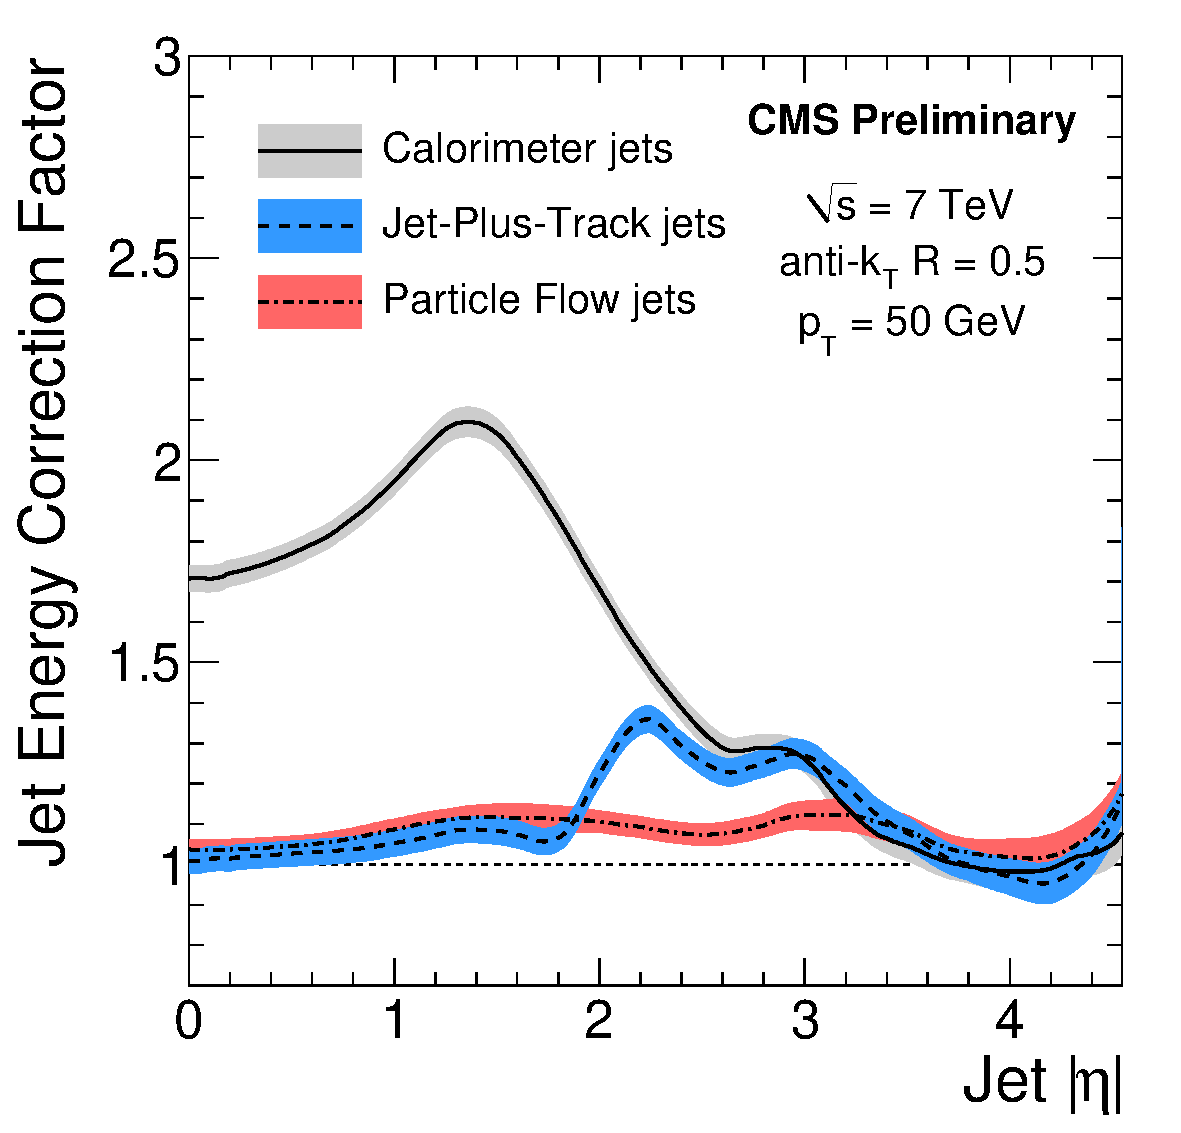
\includegraphics[width=0.45\textwidth]{fig/jet_energy_corr_pt50.pdf}}\quad
  \subfloat[\unit{200}{\GeV}]{\label{fig:jet_energy_corr_200}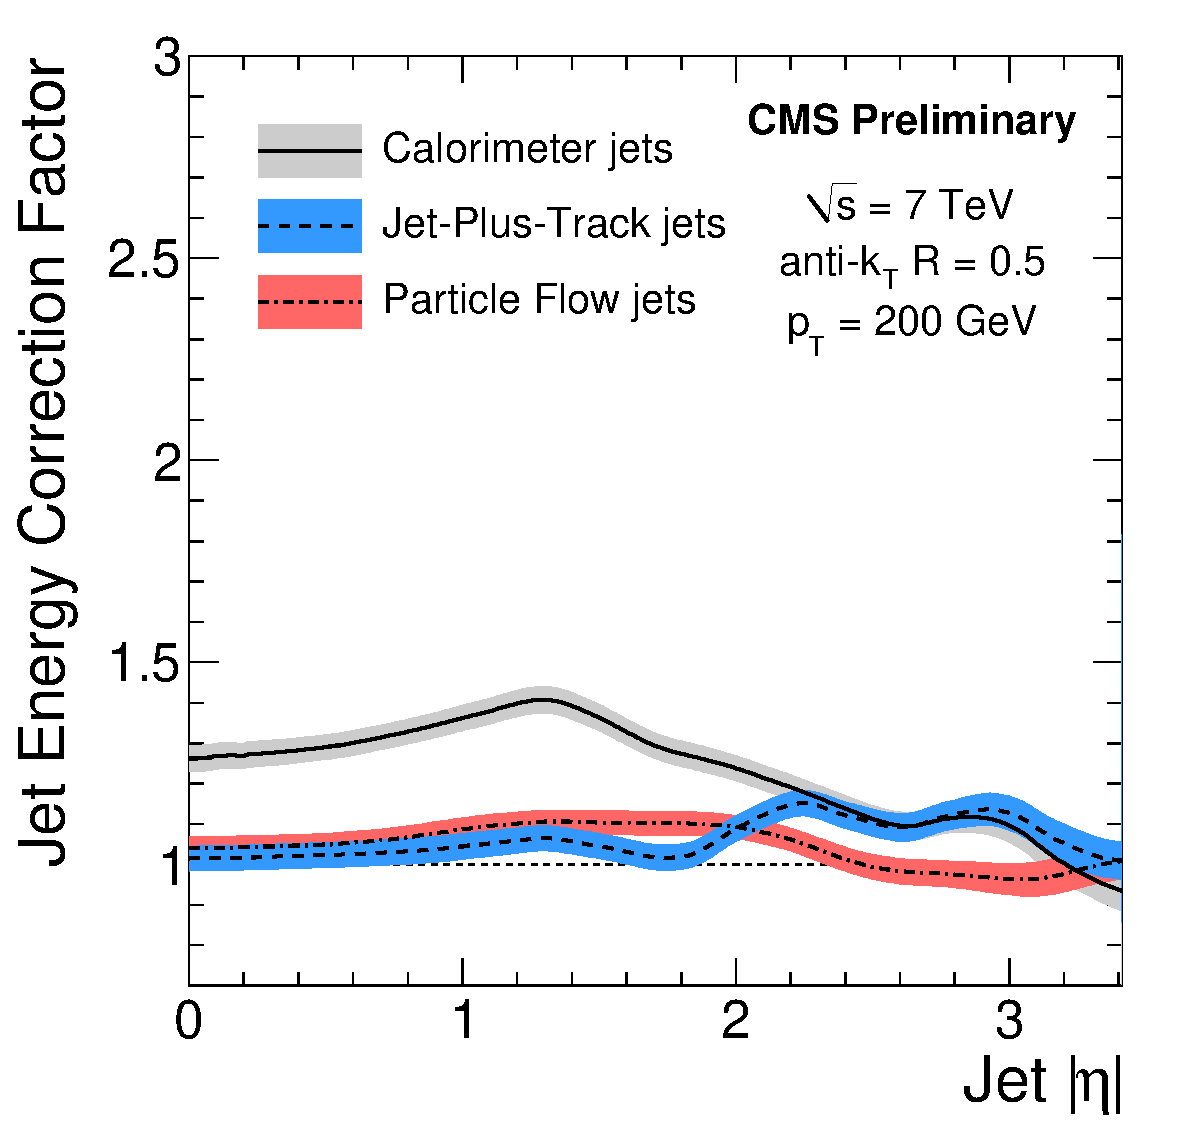
\includegraphics[width=0.45\textwidth]{fig/jet_energy_corr_pt200.pdf}}\quad
  \caption[Total jet energy correction factor as a function of $\eta$ for jets
  with transverse momenta of \unit{50}{\GeV} and \unit{200}{\GeV}]{Total jet
    energy correction factor as a function of $\eta$ for jets with transverse
    momenta of \unit{50}{\GeV} and \unit{200}{\GeV}. Corrections are shown for
    \ac{Calo}, \ac{JPT} and \ac{PF} jets separately. The bands indicate the
    corresponding uncertainties~\cite{jet_energy_pas}.}
  \label{fig:reco_jet_energy_corr}
\end{figure}

\section{Missing Energy}
Certain particles, such as neutrinos, are not reconstructed by the \ac{CMS}
detector. However, their presence may be inferred by considering the total
momentum of particles reconstructed by the detector and comparing this with the
momentum of the initial state. Any imbalance in these quantities can be
attributed to the presence of some ``invisible'' particles - a \emph{missing
  energy} signature.

At a hadron collider, the situation is complicated by the fact that the boost of
the initial partons parallel to the beamline is not known. Hence missing energy
measurement along this axis is not possible. For this reason, transverse
quantities are used instead - most commonly the \emph{missing transverse
  energy}, \METv. This can be defined generically as
\begin{equation*}
\METv = -\sum_{o in \textrm{objects}} \vec{p}_T^o,
\end{equation*}
where $p_T^o$ refers to the transverse momentum of object $o$. The chosen set of
objects then leads to a number of alternative definitions of \METv. The
magnitude of this quantity, often used in event selection, will be denoted
\MET. Similar notation will be used for other transverse vector quantities.

At \ac{CMS}, the simplest measurement of \METv is \ac{Calo} \METv which sums
over the calorimeter tower energies (\ac{ECAL} and \ac{HCAL}).  An energy
threshold is applied to the towers in order to reject electronics
noise. Alternatively, \ac{PF} \METv sums over the candidate particles output by
the \ac{PF} algorithm. This will be discussed further in
Section~\ref{sec:reco_pf}. As will be seen, this provides the most sensitive
\METv measurement at \ac{CMS} and thus is used throughout the work presented
here. It should be assumed, unless noted otherwise, that references to \METv or
derived quantities use the \ac{PF} measurement.

Alternative missing energy quantities can be defined for other purposes. Often,
a scalar quantity is desired instead. The \emph{missing transverse hadronic
  energy} (\MHT) is formed by taking the vector sum,
\begin{equation*}
\MHTv = -\sum_{j \in \textrm{jets}} \vec{E_T^j}.
\end{equation*}
In general, this is used to measure the energy of a system of particles
recoiling against the jets in an event. For example, in \Wjets events, the
recoiling system is the \PW boson. \MHTv is therefore one possible measurement
of the \PW boson transverse momentum, \PtWv.


\section{Particle Flow at \ac{CMS}}
\label{sec:reco_pf}
The \ac{PF} algorithm~\cite{cms_pf_pas, cms_pf_pas2} attempts to provide a
global reconstruction of the event - accurate determination of the type, energy
and direction of all stable particles - by combining measurements from all
subdetectors in \ac{CMS}. This strategy is well suited for use with the \ac{CMS}
detector. The silicon tracker is able to reconstruct charged particle tracks
with high efficiency and purity down to transverse momenta as low as
\unit{150}{\MeV}. Additionally, the granularity of the \ac{ECAL} is sufficient
for the separation of photons and charged particle energy deposits in jets with
\Pt of a few hundred \GeV~\cite{cms_pf_pas}. In contrast, the \ac{HCAL} is much
coarser. However, the combined energy resolution of both calorimeters is $\sim
10\%$ at \unit{100}{\GeV}. This allows identification of the energy deposits
associated with neutral hadrons as an excess on top of that accounted for by
matching the deposits with charged tracks. The \ac{PF} algorithm is able to
reconstruct the components of jets and hadronic tau decays - primarily charged
hadrons, neutral hadrons and photons. This provides an improved measurement of
the jet energy and thus also of \METv.

The particle flow algorithm proceeds by linking the tracks and energy clusters
to form blocks. A typical event display illustrating this process is shown in
\fig~\ref{fig:reco_pf_diag}. A single block may contain some combination of a
charged particle track, one or more energy clusters and a muon. The fine
granularity of the \ac{CMS} detector ensures that blocks typically contain 1, 2
or 3 elements.  The links between each block are parameterised by a distance
which encodes the quality of the link. Advanced tracking and calorimeter
clustering algorithms have been developed to meet the needs of the \ac{PF}
algorithm. These will now be explained.

\begin{figure}[h!]
\centering
\subfloat[]{\label{fig:reco_pf_diag1}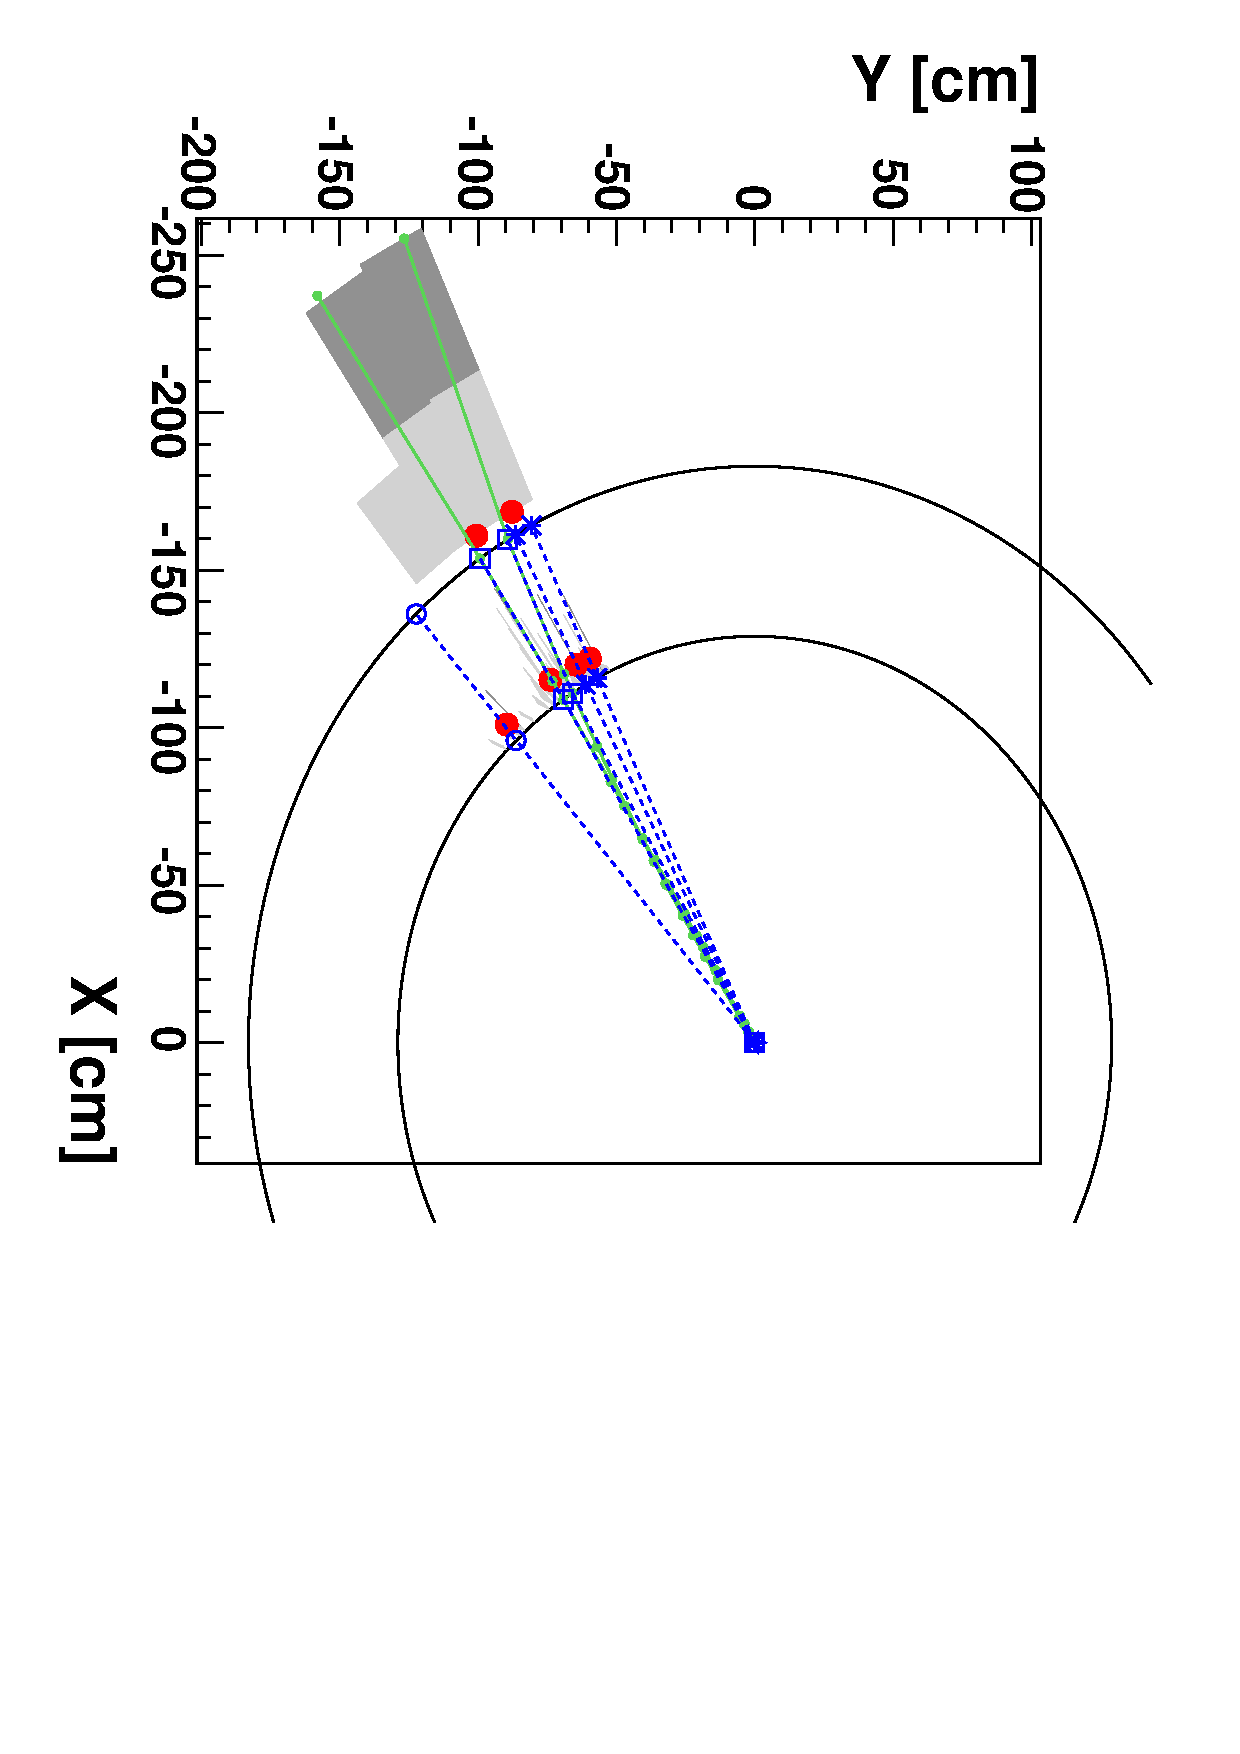
\includegraphics[width=0.7\textwidth]{fig/pf_diag1}}\\
\subfloat[]{\label{fig:reco_pf_diag2}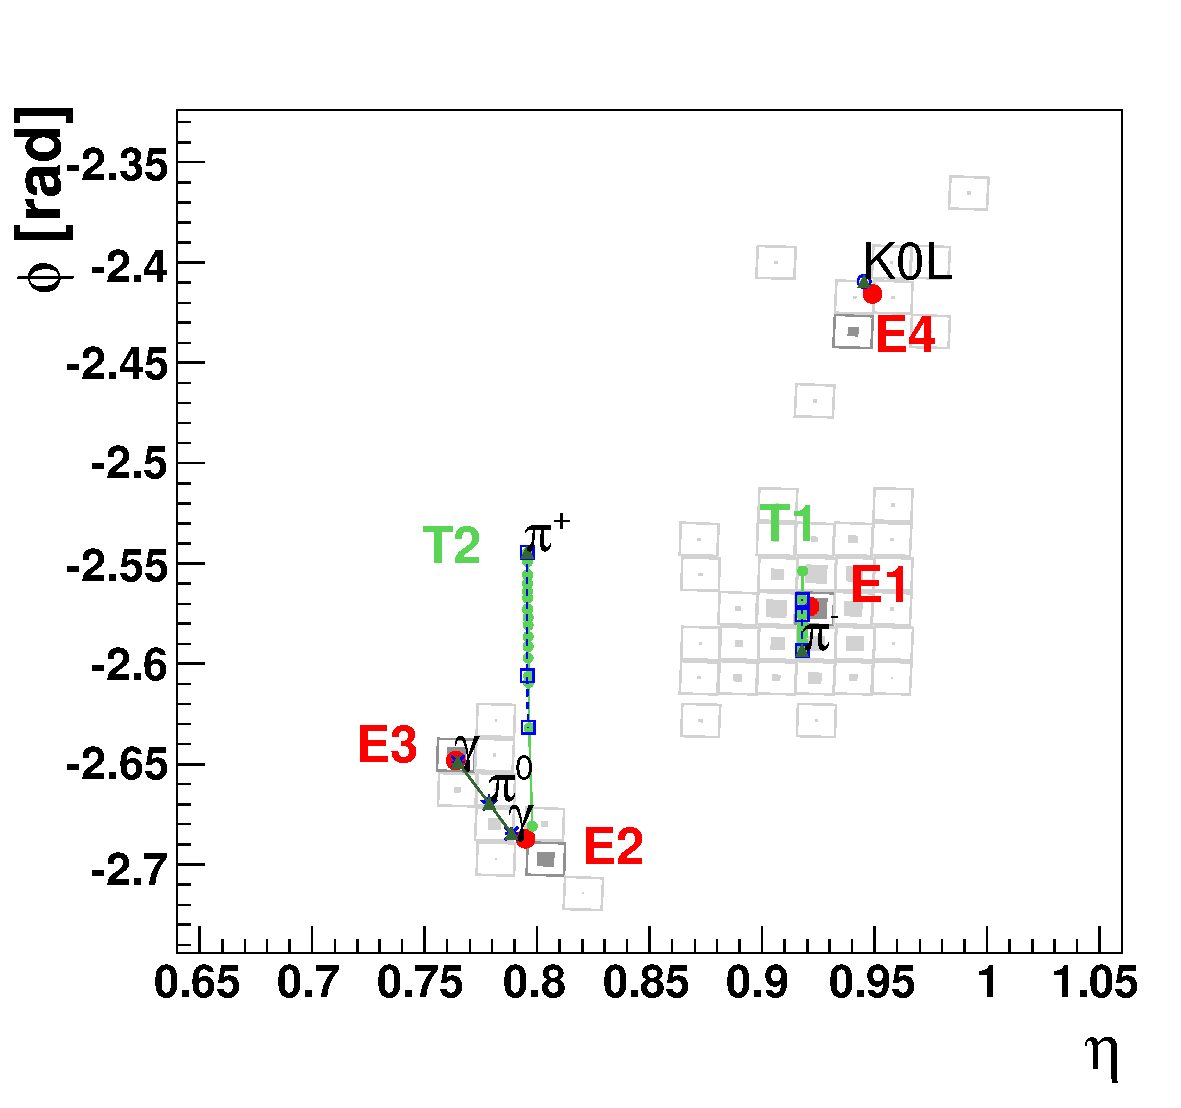
\includegraphics[width=0.45\textwidth]{fig/pf_diag2}}\quad
\subfloat[]{\label{fig:reco_pf_diag3}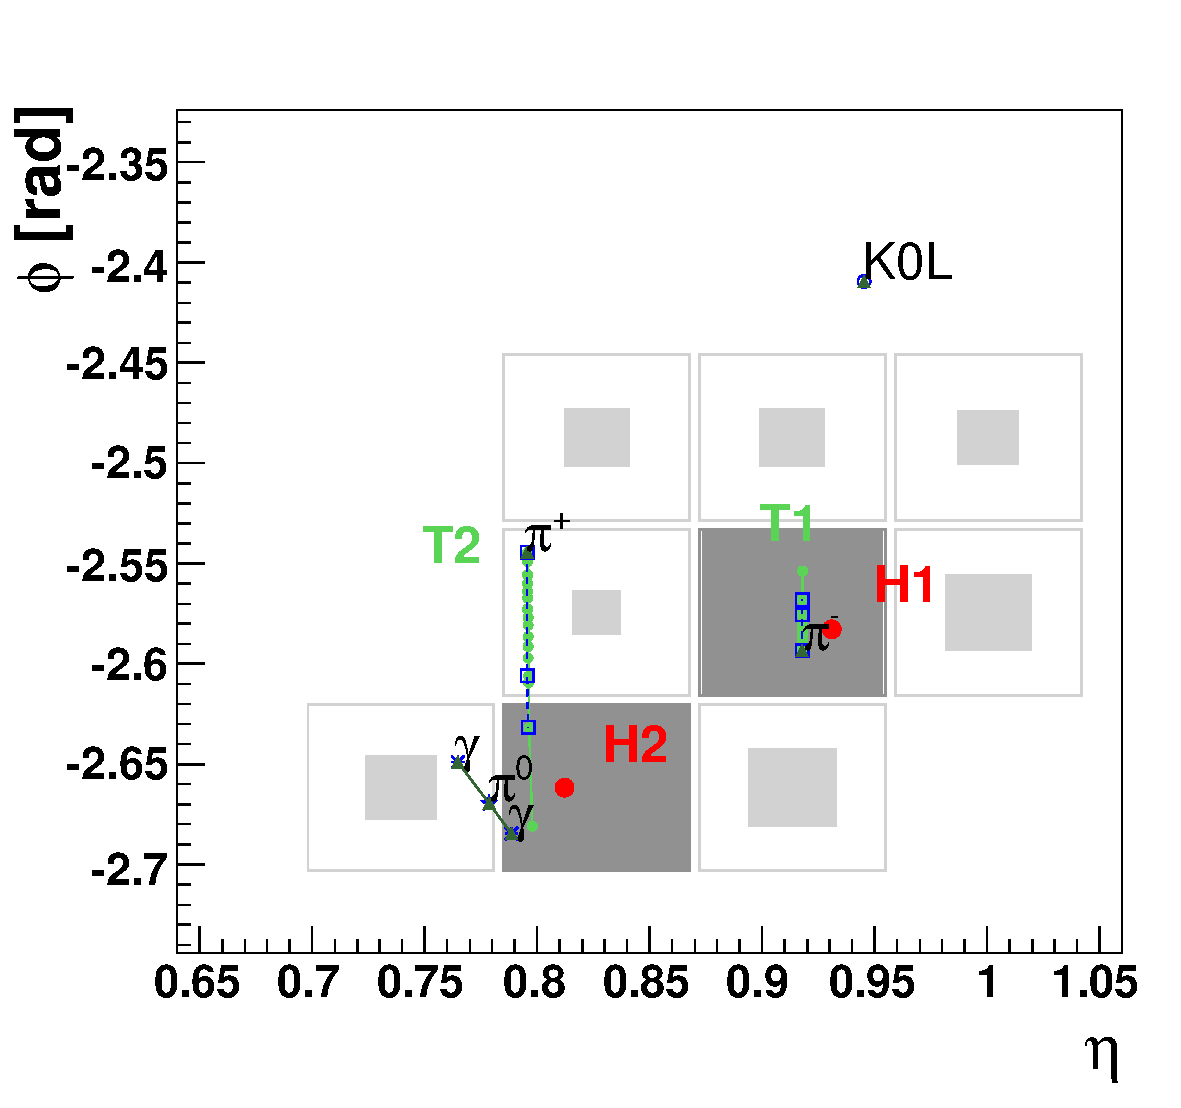
\includegraphics[width=0.45\textwidth]{fig/pf_diag3}}
\caption[]{An event display showing a hadronic jet in~\subref{fig:reco_pf_diag1}
  the $(x,y)$-plane, \subref{fig:reco_pf_diag2} an $(\eta,\phi)$ view at the
  surface of the \ac{ECAL} and~\subref{fig:reco_pf_diag3} the same orientation
  at the surface of the \ac{HCAL}. These two surfaces appear as circular arcs
  in~\subref{fig:reco_pf_diag1}. The \PKlong, \Ppiminus, \Ppiplus, \Ppizero and
  the two photons from its decay are shown. The \PKlong, \Ppiminus and two photons
  result in clear, well-speparated \ac{ECAL} cluters - round points labelled E1
  to E4~\ref{fig:reco_pf_diag2}. The \Ppiplus and \Ppiminus are reconstructed as
  charged tracks - green lines labelled T1 and T2 - which point to the two
  \ac{HCAL} clusters - round points labelled H1 and H2~\cite{cms_pf_pas}.}
\label{fig:reco_pf_diag}
\end{figure}

\subsection{Iterative Tracking}
The measurements of momentum and direction of charged hadrons provided by the
tracker are hugely superior to those that can be provided by the calorimeters.
It is important therefore that the tracks input to the \ac{PF} procedure be
reconstructed with near 100\% efficiency. The fake rate must also be low to
avoid excess energy counting.

To meet these requirements, tracks are reconstructed using an iterative
algorithm. This begins by reconstructing tracks with very tight selection
requirements. Hits which can be unambiguously assigned in this step are then
removed from consideration. The algorithm is iterated, attempting to reconstruct
tracks from the remaining hits, this time with loosened selection criteria. This
procedure is repeated with progressively looser selection criteria. This ensures
high efficiency, whilst the removal of hits at each stage reduces the fake rate
induced by combinatorics.  After three iterations, tracks originating close to
the beam line are reconstructed with an efficiency of 99.5\% for muons and
$>90\%$ for charged hadrons. The fourth and fifth iterations relax constrains on
the vertex, reconstructing secondary charged particles.

\subsection{Calorimeter Clustering}
The success of the \ac{PF} reconstruction is dependent on certain aspects of the
clustering algorithm. In particular, as for the tracks, the clustering needs to
be highly efficient and be able to distinguish closely spaced energy deposits.
To this end, a specialised clustering algorithm was developed. This algorithm is
used the \ac{ECAL}, \ac{HCAL}, \ac{PS} but not in the \ac{HF} where each cell is
taken to be a cluster.

The first step of the algorithm produces \emph{seed clusters} from local maxima
in the calorimeter cell energies meeting a minimum threshold requirement.  These
seed clusters are then extended to include cells sharing at least one side in
common with the original cluster and an energy exceeding a threshold chosen
according to the standard deviation of electronics noise in the
calorimeter. These \emph{topological clusters} are then transformed into
\emph{particle flow clusters}, with a separate particle flow cluster for each
seed comprising the topological cluster. The energy and position of each
particle flow cluster is determined iteratively, with the energy of each cell
shared among the particle flow clusters.

\subsection{Building Links}
Each track is extrapolated from the position of its last measured hit to the
\ac{PS}, the \ac{ECAL} at a depth corresponding to the expected maximum for an
electron shower, the \ac{HCAL} at a depth of 1 interaction length. If the
extrapolated track position lies within the envelope of a cluster, a link is
created with a link distance equal to the $(\eta, \phi)$ distance between the
extrapolated track and the cluster. The envelope may be enlarged with respect to
the cluster by the extent of a single cell.

Additionally, energy contributions from bremsstrahlung photons are included by
extrapolating the track tangent at each tracker layer to the \ac{ECAL}. If the
extrapolated track lies within the envelope of the cluster, a link is created.
Links are also created between calorimeter clusters in different subdetectors if
the cluster position in the finer-grained calorimeter lies within the envelope
of the more coarsely grained calorimeter. The link distance is taken to be the
$(\eta, \phi)$ separation of the two clusters.

Muons are included when a global fit between a track in the tracker and a muon
track in the muon chambers yields an acceptable \chisq. If several global muons
are found for a single muon track, only that possessing the smallest \chisq is
retained - with the link distance determined by the \chisq.

\subsection{Particle Reconstruction}
The first step is to reconstruct muons. Each global muon gives rise to a
particle flow muon providing its momentum as determined from the global fit is
compatible with the track momentum to within 3 standard deviations. The
corresponding track is then removed from the block.

The next step is electron reconstruction. Electron tracks in the block are first
selected by a pre-identification step - electrons often leave short tracks and
lose energy via bremsstrahlung. Pre-identified electrons are then refit with a
Gaussian Sum Filter (see Section~\ref{sec:reco_electrons}) and projected into
the \ac{ECAL}.  Candidates passing tracking and calorimetric criteria are
reconstructed as particle flow electrons. The track and associated \ac{ECAL}
clusters are then removed from the block.

Tracks remaining are then subject to a tighter set of quality requirements, in
particular that the track \Pt uncertainty be smaller than the relative
calorimeter energy resolution for a charged hadron. Whilst some real hadrons are
lost by this requirement, the energy will be retained in the more accurate
measurement of the calorimeter.

Reconstruction of photons and neutral hadrons involves comparison of the track
momentum to the calorimetric energy. The cluster energies in the \ac{ECAL} are
calibrated for photons and the \ac{HCAL} for \unit{50}{\GeV} pions. For the
comparison to be valid, these must be re-calibrated to account for
non-linearities in the \ac{HCAL} as well as the differing response of the
\ac{ECAL} to hadrons.

In the case that several tracks are linked to a single \ac{HCAL} cluster, the
total momenta of the tracks is compared to the calibrated calorimetric energy.
Tracks linked to multiple clusters are resolved by preserving the closest link
or links in certain cases. The track momentum is then compared to the total
calibrated calorimetric energy.

In the rare case that the energy is smaller than the track momentum by more than
three standard deviations, a relaxed search for fake tracks and global muons is
initiated. Global muons are identified as \ac{PF} muons if their momentum is
measured with an uncertainty below 25\%. Tracks are then progressively removed
from the block, those with largest momentum uncertainty first, until either all
tracks with an uncertainty $>\unit{1}{\GeV}$ have been considered or the total
track momentum has decreased below the calorimetric energy. The remaining tracks
are interpreted as charged hadrons with momentum and energy taken from the track
momentum assuming the charged pion mass hypothesis. If the calorimeter energy
and track momentum are compatible within their uncertainties, the momentum is
redefined by a fit to both track momenta and the energy cluster. This is helpful
at very high energies, where the track parameters may be less well measured.

In the case that the calibrated energy is greater than the total track momentum
by more than the calorimetric energy resolution, the excess is interpreted as
a photon and possibly a neutral hadron. If the excess is greater than the
\ac{ECAL} energy, a photon is created with this energy and the rest of the
excess interpreted as a neutral hadron. Otherwise, a photon only is
reconstructed from the uncalibrated \ac{ECAL} energy. This stems from the
observation that photons carry 25\% of the energy of a jet, with neutral hadrons
only 3\%.

Remaining \ac{ECAL} and \ac{HCAL} clusters not linked to a track (or for which
the associated track was disabled in the previous steps) are reconstructed as
photons and neutral hadrons respectively.

\ac{PF} jets are reconstructed by applying the \antikT algorithm to the full set
of \ac{PF} objects.

\subsection{Physics Performance}
Two aspects of the performance of the \ac{PF} reconstruction are of relevance to
the analysis description that will follow: measurement of \METv and jet
reconstruction.

\begin{figure}
\centering
\subfloat[]{\label{fig:reco_pf_jet_energyres_barrel}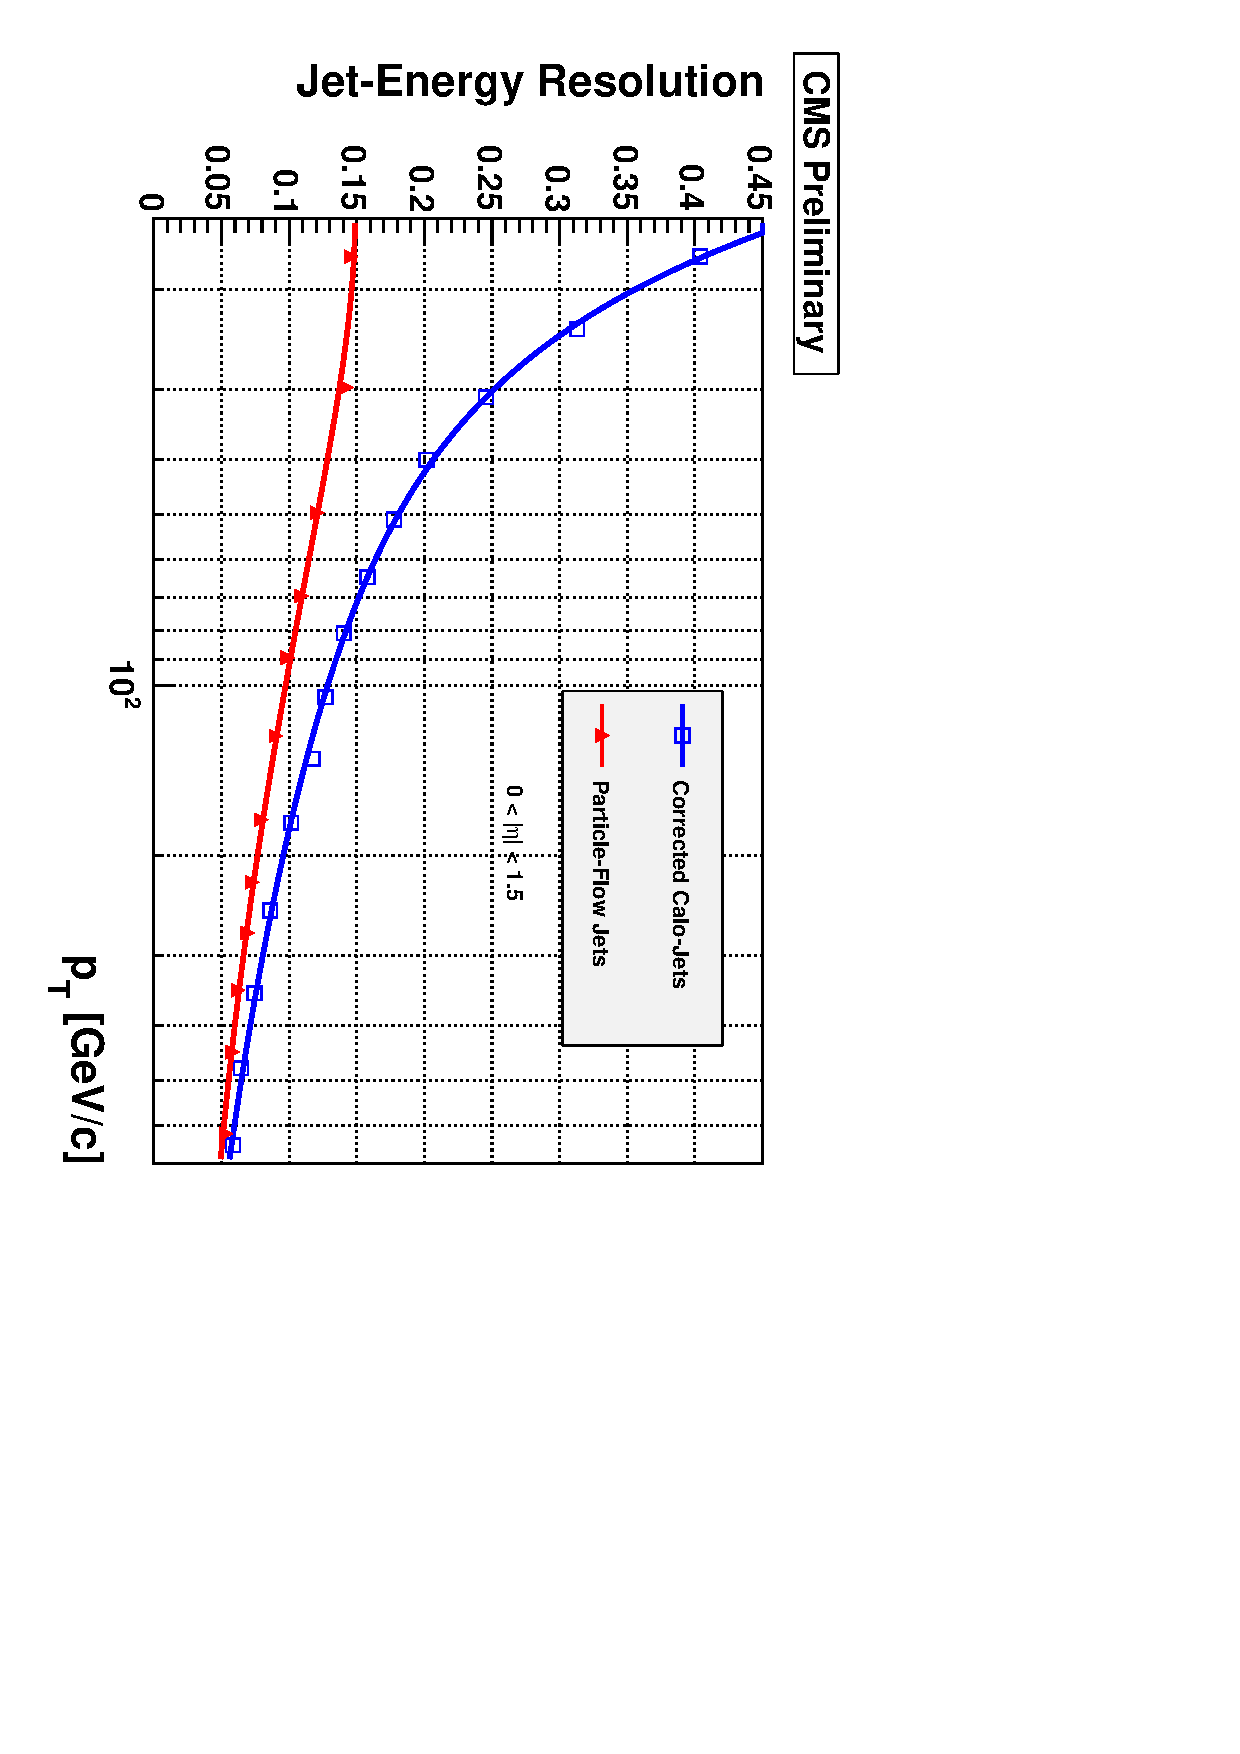
\includegraphics[width=0.45\textwidth]{fig/pf_jet_energyres_barrel}}\quad
\subfloat[]{\label{fig:reco_pf_jet_energyres_endcap}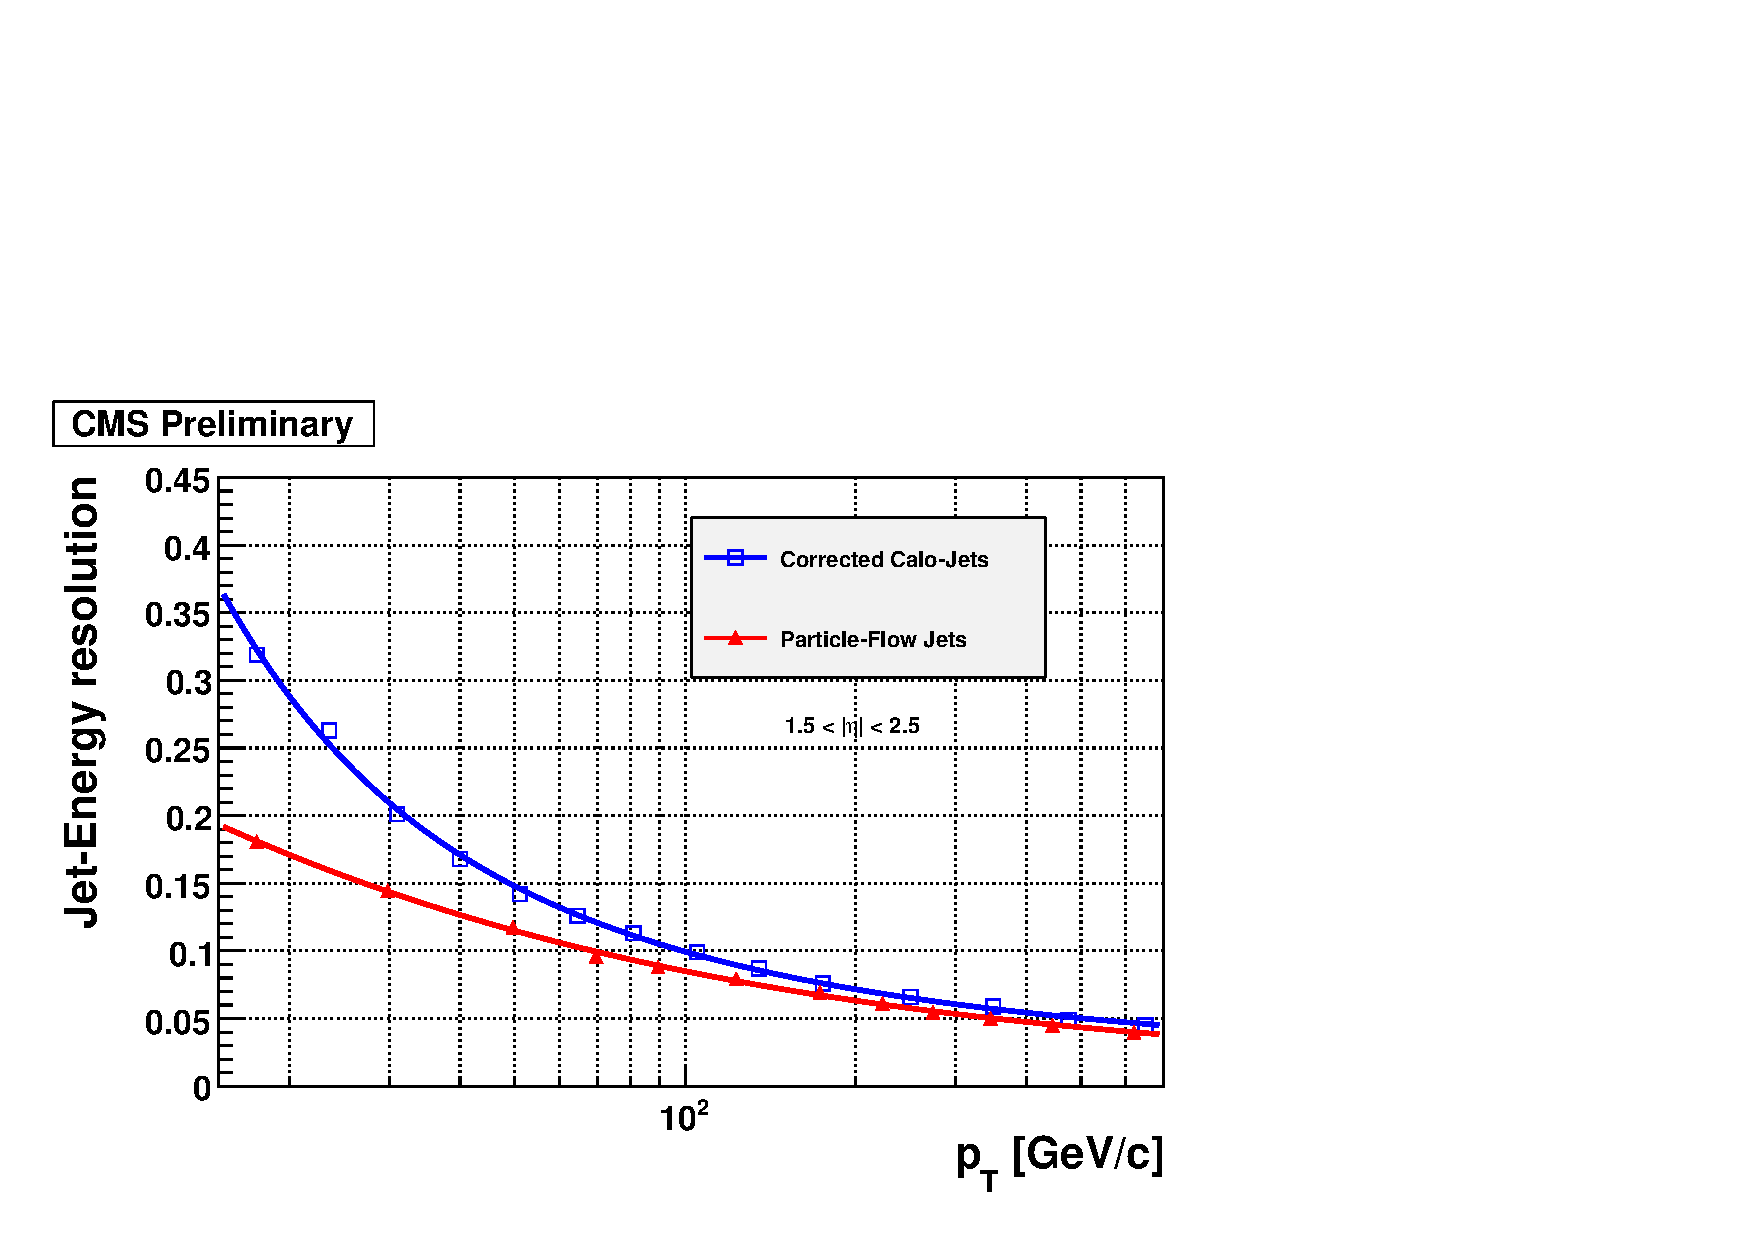
\includegraphics[width=0.45\textwidth]{fig/pf_jet_energyres_endcap}}\quad
\caption[Jet energy resolution as a function of \Pt]{Jet energy resolution as a
  function of \Pt for the \subref{fig:reco_pf_jet_energyres_barrel} barrel and
  \subref{fig:reco_pf_jet_energyres_endcap} endcap. Calo-jet values are
  displayed as open squares and \ac{PF} jet as upwards triangles. The curves are
  fit to the sum of a constant term, a stochastic term and a noise term.}
\label{fig:reco_pf_jet_energyres}
\end{figure}

\begin{figure}
\centering
\subfloat[]{\label{fig:reco_pf_jet_etares}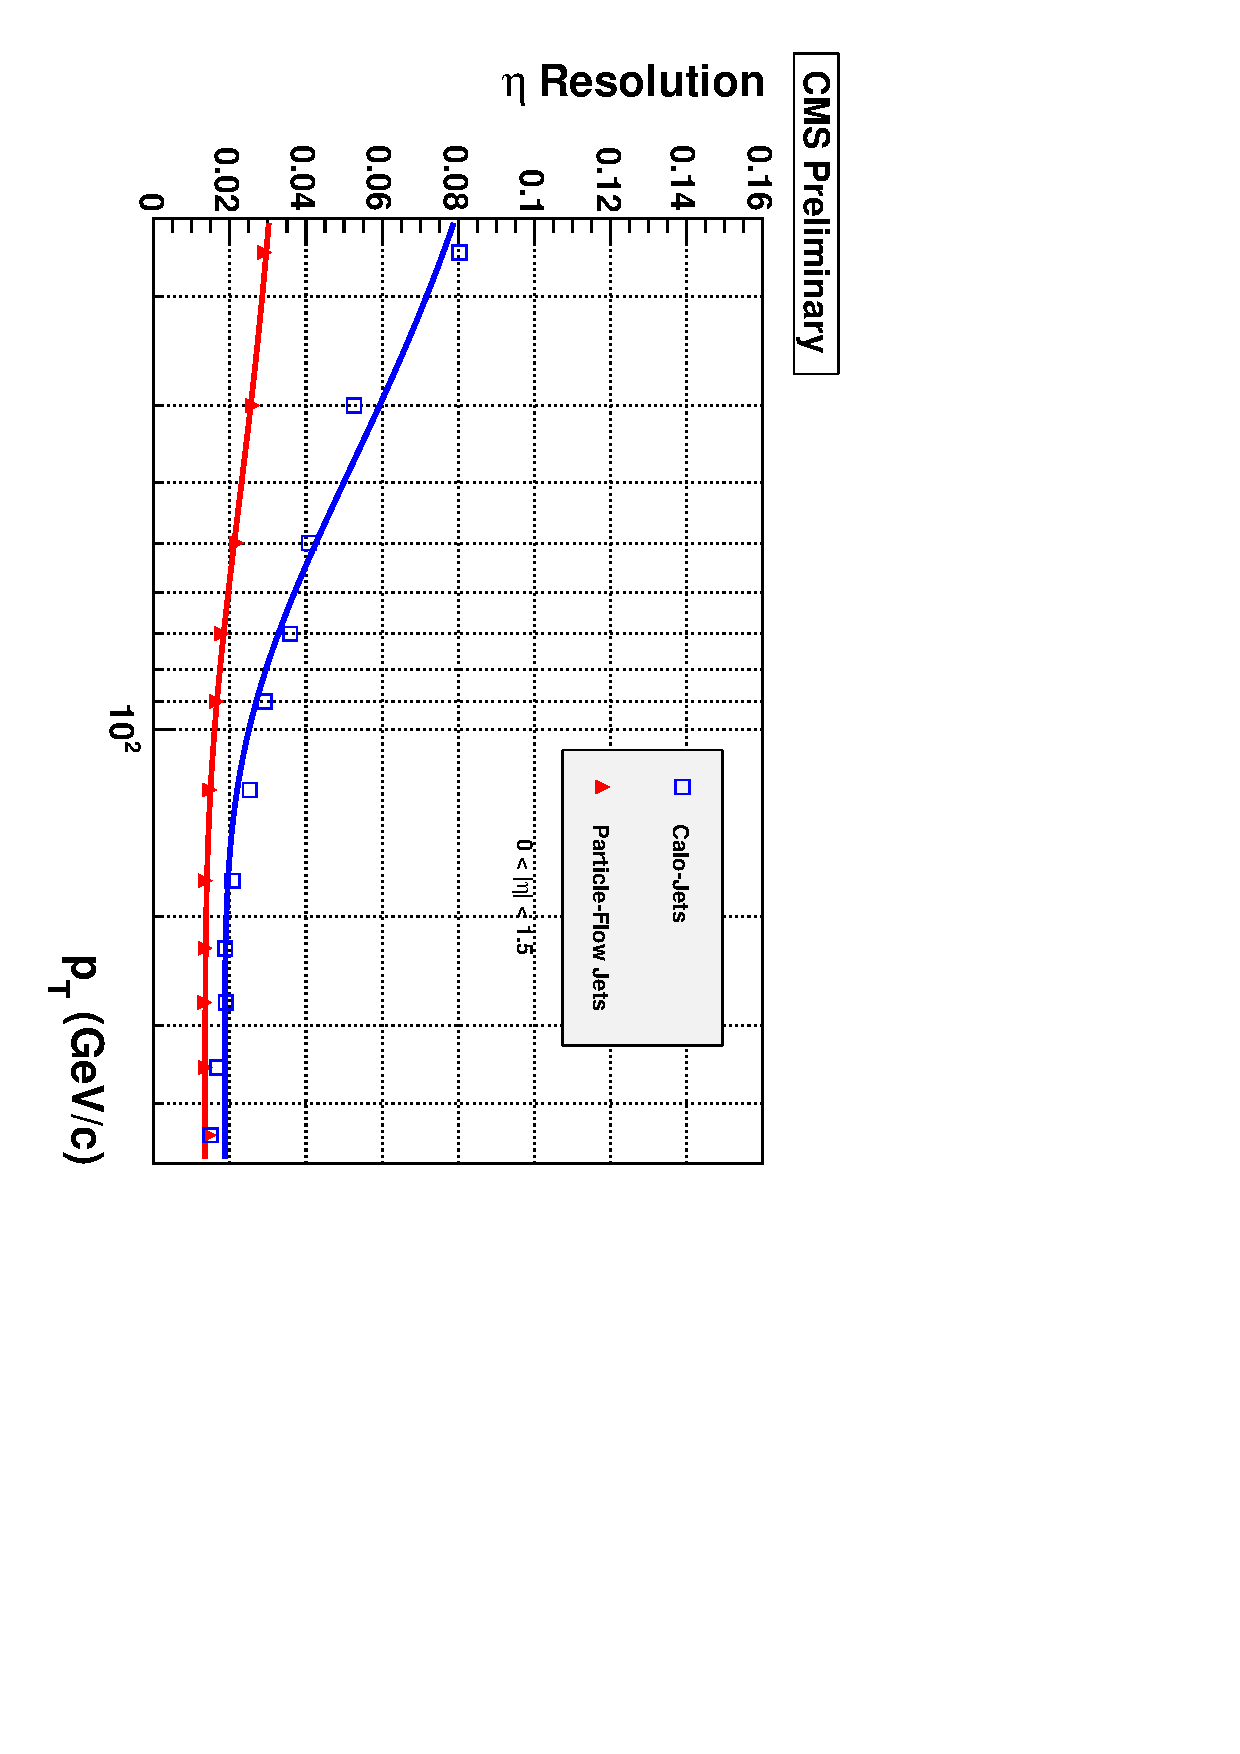
\includegraphics[width=0.45\textwidth]{fig/pf_jet_etares}}\quad
\subfloat[]{\label{fig:reco_pf_jet_phires}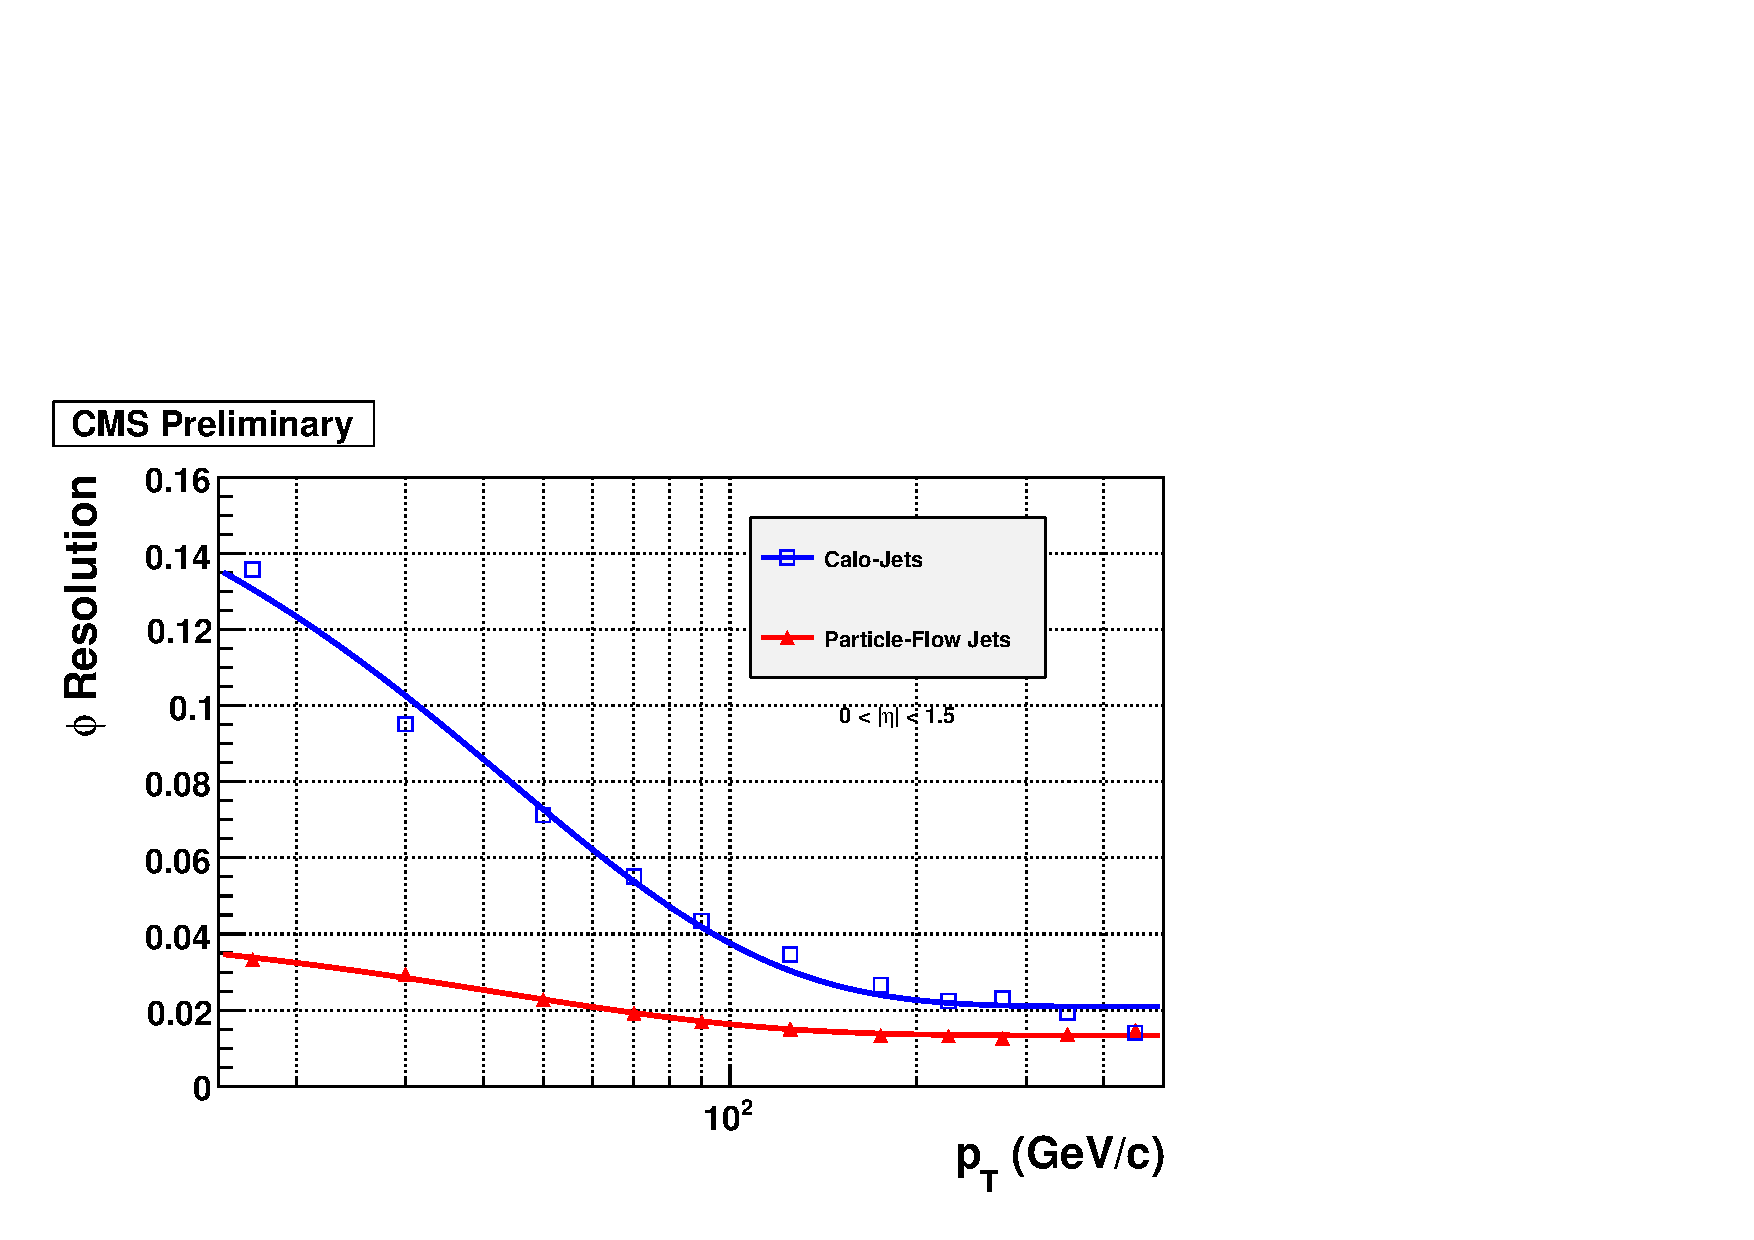
\includegraphics[width=0.45\textwidth]{fig/pf_jet_phires}}\quad
\caption[Jet angular resolution (\ac{RMS}) as a function of \Pt]{Jet angular
  resolution (\ac{RMS}) as a function of \Pt for \subref{fig:reco_pf_jet_etares}
  $\eta$ and \subref{fig:reco_pf_jet_phires} $\phi$. Calo-jets are shown as open
  squares and \ac{PF} jets as upward triangles. The curves are fit with an
  exponential function of $\Pt$.}
\label{fig:reco_pf_jet_angulares}
\end{figure}

\begin{figure}
\centering
\subfloat[]{\label{fig:reco_pf_met_metres}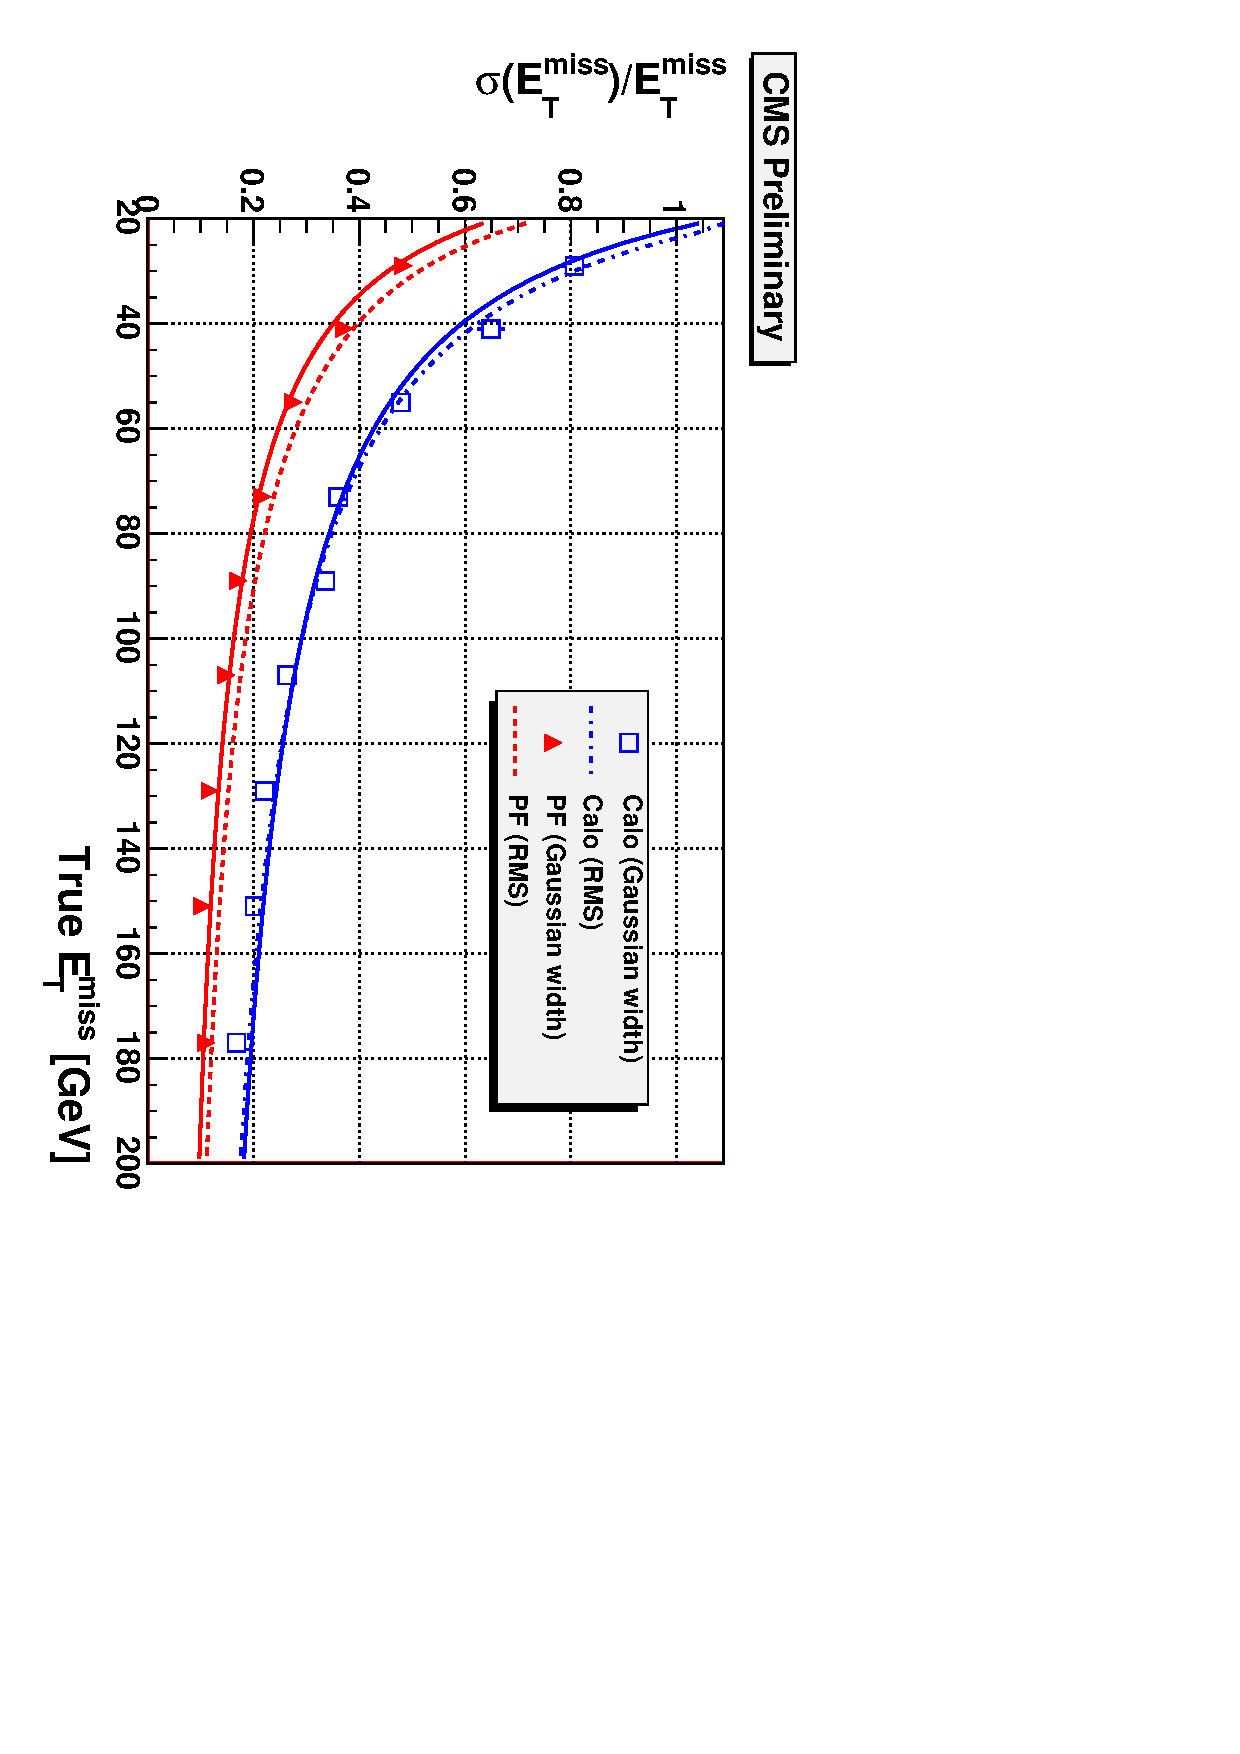
\includegraphics[width=0.45\textwidth]{fig/pf_met_metres}}\quad
\subfloat[]{\label{fig:reco_pf_met_phires}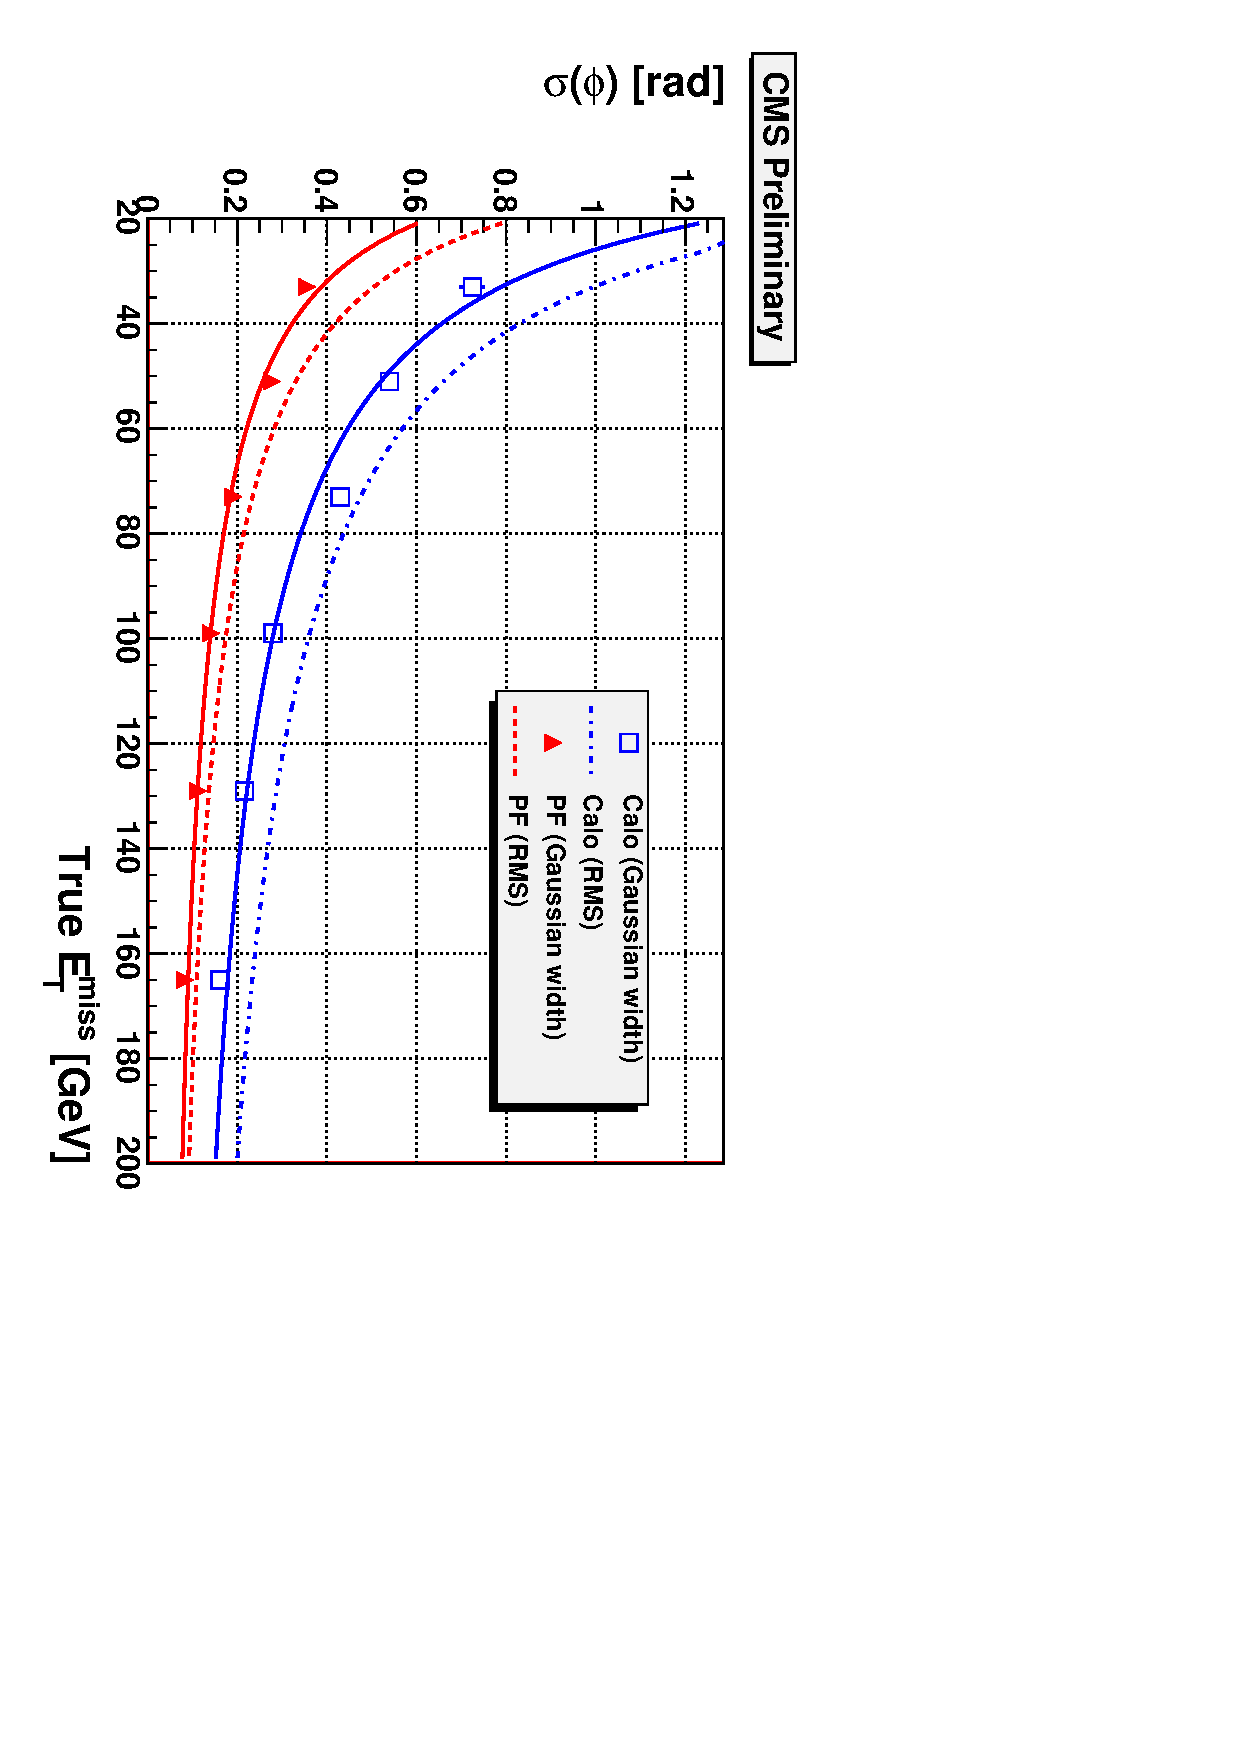
\includegraphics[width=0.45\textwidth]{fig/pf_met_phires}}\quad
\caption[\MET Resolution]{\subref{fig:reco_pf_met_metres}$\sigma(\MET)/\MET^{\textrm{true}}$ and
  \subref{fig:reco_pf_met_phires} $\sigma(\phi)$ as a function of true \MET in
  \ttbar events as determined by a Gaussian fit to each $\MET^{\textrm{true}}$
  bin. Squares represent Calo-\MET, and upwards triangles \ac{PF} \MET. The
  solid curves ares fits through these points. The dashed lines indicate the
  \ac{RMS} width of each bin.}
 \label{fig:reco_pf_met_res}
\end{figure}

  \chapter{Measurement of the Polarisation of the \texorpdfstring{\PW}{W} Boson}
\label{sec:wpol}
\section{Introduction}
The study of \Wjets production at a hadron collider is an important avenue for
the further undestanding of the underlying \ac{EWK} and \ac{QCD} processes. In
particular, since it is one of a relatively small number of processes for which
highly precise \ac{NLO} calculations have been performed (see
\sec~\ref{sec:framework_vboson}), experimental measurements can provide
constraints on the \acp{PDF}. \Wjets production is also of considerable interest
in the context of \ac{NP} searches where these events are often a significant
background. Finally, in the leptonic decay mode, the neutrino provides a source
of ``real'' missing-energy. This is useful in the understanding of detector
effects relevant to searches for the \acs{WIMP} particles that are present in
\ac{SUSY} and other theories.

\section{Measuring the Helicity Fractions of the \texorpdfstring{\PW}{W} Boson}
\subsection{Generator and Simulation Level Expectations}
As will become clear, any measurement of the helicity fractions will depend to
some extent on \acl{MC} input. Therefore, it is important to study the effect,
both at the generator-level, and at the level of reconstructed simulated
events. This firstly ensures that the expected effects are adequately modelled
by the chosen \ac{MC} generator and secondly allows the testing of the
theoretical expectations in the context of ``real'' detector-level
quantities. This is vital to ensure that the measurebmenbt of helicity fractions
is actually feasible and not washed out by some experimental effect.

Unless otherwise noted, the \Wjets samples used is produced using the
\madgraph~\cite{madgraph} generator interfaced to \pythia version
6~\cite{pythia}. The generated sample comprised approximately 15 million events
with the \acp{PDF} taken from the \cteqsixlone set within the \lhapdf software
package~\cite{lhapdf, lhapdf_web}.

Shown in \fig~\ref{fig:wpol_costheta} are $\cos\thetastar$ distributions at
generator level in bins of \PtW for \PWp along with a fit to
\eqn~\ref{eqn:wpol_helicity_fractions}. The polarisation is manifest in the
dominance of the $(1-\cos\thetastar)^2$ term, leading to the peak at
$\cos\thetastar = -1$. This reflects the fact that the left-handed particle (the
neutrino in this case) is taking most of the energy. Similarly for \PWm, the
peak is at $\cos\thetastar = 1$, where this time the electron is more energetic.

\begin{figure}[h!]
\centering
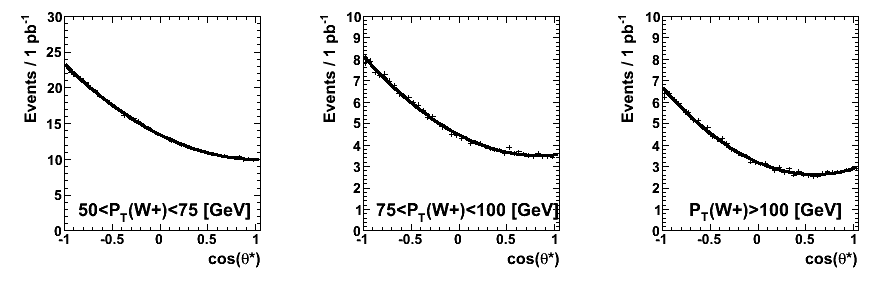
\includegraphics[width=0.98\textwidth]{fig/MC_CosThetaStar1Plus}
\caption{Distribution of $\cos\thetastar$ for \PWp bosons in three bins of \PtW.}
\label{fig:wpol_costheta}
\end{figure}

\begin{figure}[h!]
\centering
\subfloat[$\PtW > \unit{200}{\GeV}$]{
  \label{fig:wpol_costheta_corr200}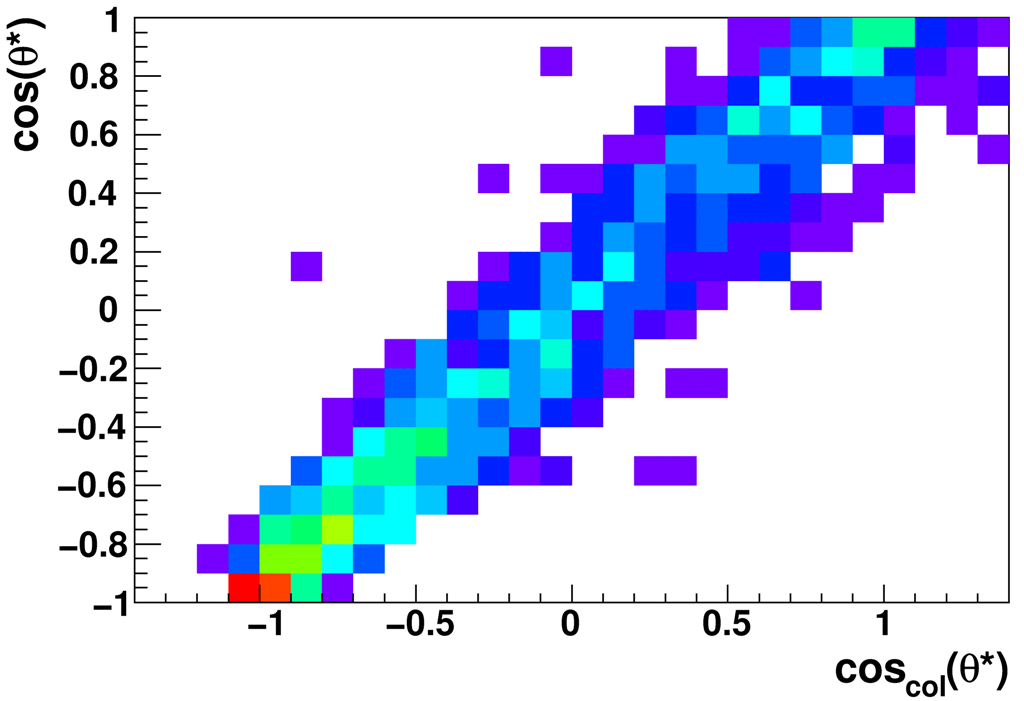
\includegraphics[width=0.47\textwidth]{fig/LP_corr200}}\quad
\subfloat[[$\PtW > \unit{400}{\GeV}$]{
  \label{fig:wpol_costheta_corr400}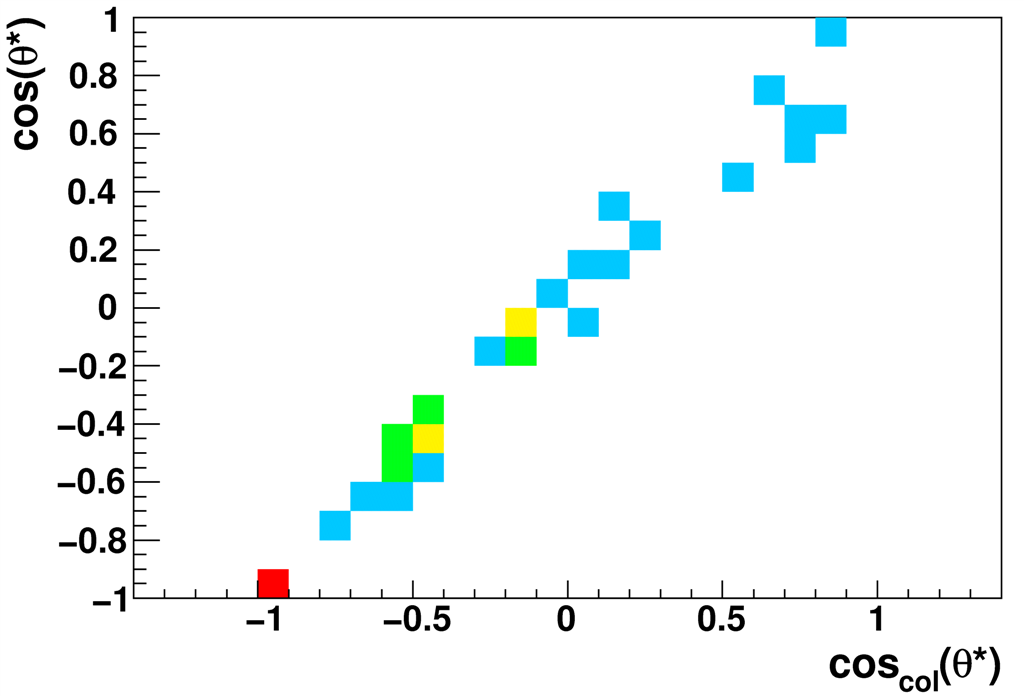
\includegraphics[width=0.47\textwidth]{fig/LP_corr400}}\quad
\caption{Correlation of $\cos\thetastar$ and $2\LP - 1$ for \PW bosons in
  simulation. The correlation is shown for two different cuts on the transverse
  momentum, \PtW.}
\label{fig:wpol_costheta_corr}
\end{figure}

\subsection{The Lepton Projection Variable}
\label{sec:wpol_lp}
In order to calculate the value of $\cos\thetastar$, the \PW rest frame must be
reconstructed. This requires knowledge of both the charged and neutral lepton
momenta. At a hadron collider, the neutrino escapes undetected and is
reconstructed as a missing energy signal. This involves taking the vector sum of
all observed particle momenta and using momentum conservation arguments to infer
that any remaining momentum imbalance is due to the missing neutrino. At a
hadron collider, the boost of the colliding partons is not known and thus, the
component of the neutrino momentum parallel to the beam line cannot be inferred
from the missing momentum. This prevents unique determination of the \PW
momentum, introducing a two-fold ambiguity on the measurement of $P^{\PW}_z$ and
thus making it impossible to fully reconstruct the helicity frame. Although the
possibility exists of either picking one solution and applying correction
factors for the error this causes in the results or taking both solutions and
weighting them using simulated data, these introduce a great deal of
complexity. Instead, a variable is chosen which is known to be highly correlated
with $\cos\thetastar$ at suitably high $\PtW$ and yet also directly calculable
from transverse detector-level quantities. This variable is the Lepton
Projection variable or \LP and is defined as follows~\cite{wpol_an, jad_thesis},
\begin{equation}
\label{eqn:lp_def}
  \LP = \frac{\Ptlv.\PtWv}{\left|\PtWv\right|^2},
\end{equation}
where \Ptlv and \PtWv are the transverse momenta of the charged lepton and \PW
boson respectively and $\PtWv = \Ptlv +\METv$.

\subsubsection{Correlation with \boldmath{$\cos\thetastar$}}
To motivate the use of the \LP variable in measuring $\cos\thetastar$ at high
\PtW, the correlation can be demonstrated analytically. Consider the decay
lepton momentum in the helicity frame,
\begin{equation*}
\mPl' = \mPl_{\parallel}' + \mPl_{\perp}',
\end{equation*}
where $\mPl_{\parallel}'$ and $\mPl_{\perp}'$ are respectively the components of
the lepton momentum parallel and perpendicular to the z-axis. Neglecting the
mass of the lepton, $\mPl' = \MW/2$, where $\MW$ is the mass of the \PW
boson. Therefore
\begin{eqnarray*}
\mPl_{\parallel}' &=& \frac{\MW}{2}\cos\thetastar \\
\mPl_{\perp}'| &=& \frac{\MW}{2}\sin\thetastar.
\end{eqnarray*}
Boosting into the lab frame (i.e. along the $-z$ axis of the helicity frame),
\begin{eqnarray*}
\mPl_{\parallel} = \gamma \frac{\MW}{2} \left (\cos\thetastar +\beta\right )
\mPl_{\perp} = \mPl_{\perp}',
\end{eqnarray*}
where $\gamma$ and $\beta$ have their usual definitions (see Appendix~\ref{app:kinematics}).

To see the correlation, we first consider the quantity $\LP^{3D}$~\cite{jad_thesis},
\begin{eqnarray*}
\LP^{3D} &=& \frac{\mPl}{\mPW} \\
&=& \frac{1}{\mPW}\sqrt{\mPl_{\parallel}^2 + \mPl_{\perp}^2}
\\
&=& \frac{\MW}{2\mPW}\sqrt{\gamma^2(\cos\thetastar +\beta)^2 + \sin^2\thetastar}\\
&=&
\frac{\MW}{2\mPW}\sqrt{\gamma^2\cos^2\thetastar + 2\gamma^2\cos\thetastar\beta
  + \gamma^2\beta^2 + \sin^2\thetastar} \\
&=&\frac{\MW}{2\mPW}\sqrt{\left(\frac{\mPW}{\MW}\right)^2\cos^2\thetastar +
  2\gamma^2\cos\thetastar\beta +\gamma^2\beta^2 +1}\\
&=&\frac{\MW}{2\mPW}\sqrt{\left(\frac{\mPW}{\MW}\right)^2\cos\thetastar^2 +
2\frac{\mPW\EW}{\MW^2}\cos\thetastar + \left(\frac{\mPW}{\MW}\right)^2 + 1}\\
&=&\frac{1}{2\mPW}\sqrt{\mPW^2\cos^2\thetastar + 2\mPW\EW\cos\thetastar + \mPW^2 + \MW^2}\\
&=&\frac{1}{2\mPW}\left(\mPW\cos\thetastar + \EW\right),
\end{eqnarray*}
where \EW is the \PW-boson energy. Rearranging it is seen that
\begin{equation*}
\cos\thetastar = 2\LP^{3D} - \frac{\EW}{\mPW}.
\end{equation*}
In the high \PtW limit, the $z$ component of the \PW can be neglected and thus
$\LP^{3D} \longrightarrow \LP$ and $\mPW \longrightarrow \EW$ so
\begin{equation*}
 \cos\thetastar \longrightarrow 2\LP - 1.
\end{equation*}
The correlation between $\cos\thetastar$ and $2\LP -1$ is shown in
\fig~\ref{fig:wpol_costheta_corr} for \PW bosons with $\PtW >
\unit{200}{\GeV}$ and $\PtW > \unit{400}{\GeV}$.

\subsubsection{Correlation with \boldmath{\phistar}}
For large \PtW, \LP is mostly uncorrelated with \phistar since even for values
$\phistar > \frac{\pi}{2}$, the lepton will still be collinear with the \PW in
the lab frame. In contrast, for low values of \PtW, the lepton in the lab frame
may have a large angular separation from the \PW. In extreme cases, the lepton
and the \PW may even be anti-parallel in the lab frame. This leads to a widening
of the \LP distribution and a much larger correlation with
\phistar.

\subsection{Template Re-weighting Method}
\label{sec:wpol_reweighting}
As has so far been described, the $\cos\thetastar$ distribution is of great
interest in the measurement of the \PW boson helicity. The \LP variable provides
a variable that is able to probe this distribution and can be calculated in a
straightforward manner from detector-level quantities. However, it has already
been seen that the $\cos\thetastar$ distribution cannot be inferred from the \LP
distribution, thus preventing a direct measurement of the helicity
fractions. In addition, the \LP distribution will be subject to a number of
detector and acceptance related effects, changing its shape.

\subsubsection{Re-weighting $\cos\thetastar$}
To account for all such experimental issues, a template re-weighting method is
employed. Effectively, \ac{MC} simulation is used to derive three
re-weighting factors, each a function of $\cos\thetastar$ and binned according
to boson charge, transverse momentum, \PtW, and rapidity, \YW. These can be
written as
\begin{equation}
\label{eqn:wpol_reweighting_factor}
Q_i\left(\cos\thetastar, \PtW, \YW, \pm \right) =
\frac{\sigma^\pm_i\left(\cos\thetastar\right)}{\displaystyle\sum_{i=-1}^{i=+1}
  \ffi^\pm\left(\PtW, \YW\right)\sigma^\pm_i\left(\cos\thetastar\right)},
\end{equation}
where the index $i$ is taken to represent the 3 helicity states of the \PW
boson. The \ffi are constants derived from an analytical fit to the
$\cos\thetastar$ distribution in bins of \PtW, \YW and charge. They are
effectively the helicity fractions ``baked in'' to the \ac{MC}. The
functional form of $\sigma$ is taken from \eqn~\ref{eqn:wpol_helicity_fractions}
as follows,
\begin{eqnarray*}
\sigma^{\pm}_{-1} &=& \frac{1}{4}\left(1\mp\cos\thetastar\right)^2\\
\sigma^{\pm}_{0}  &=& \frac{1}{2}\left(1-\cos^2\thetastar\right)\\
\sigma^{\pm}_{+1} &=& \frac{1}{4}\left(1\pm\cos\thetastar\right)^2.
\end{eqnarray*}
A given simulated event is then taken, its $\cos\thetastar$ value calculated and
a re-weighting factor derived from \eqn~\ref{eqn:wpol_reweighting_factor}
accounting for the \PtW, \YW and charge of the \PW boson. The binning is
important, as the helicity fractions are expected to vary significantly with
these parameters.

This re-weighting procedure avoids the need to generate separate \ac{MC} event
samples for each polarisation state. Using the re-weighted sample, any
distribution may be produced corresponding to a pure sample of polarised \PW
bosons. In particular, this allows the derivation of \LP shape templates which
may then be fit to the corresponding data distribution in order to extract the
helicity fractions. This ensures that all experimental and acceptance effects
can be accounted for -- providing of course that they are adequately modelled by
the \ac{MC} and detector simulation.

In reality, a small modification to \eqn~\ref{eqn:wpol_reweighting_factor} is
required to account for the finite statistical precision of the generated
sample. The functions $\sigma^{\pm}_{i}$ become instead integrals over a small
slice ($\Delta\cos\thetastar = 0.01$) of a binned $\cos\thetastar$ distribution:
\begin{equation*}
Q_i\left(\cos\thetastar, \PtW, \YW, \pm \right) =
\frac{\int_{b}^{b+\Delta\cos\thetastar}\sigma^\pm_i\left(\cos\thetastar\right)/\int_{-1}^{1}
\sigma^\pm_i\left(\cos\thetastar\right)}{
\int_{b}^{b+\Delta\cos\thetastar} \displaystyle\sum_{i=-1}^{i=+1}
\ffi^\pm\left(\PtW, \YW\right)\sigma^\pm_i\left(\cos\thetastar\right)/
\int_{-1}^{1} \ffi^\pm\left(\PtW, \YW\right)\sigma^\pm_i\left(\cos\thetastar\right)
},
\end{equation*}
where $b$ indicates a bin within the $\cos\thetastar$ distribution.

\subsubsection{\boldmath{\PtW} and \boldmath{\YW} Dependence}
Although the $\cos\thetastar$ templates for each helicity state are independent
of \PtW and \YW, the \LP templates are seen to vary. Additionally, the \ffi
parameters are also known to vary across the phase space of the \PW boson. The
intent of this analysis is to measure the \emph{average values} of these
parameters across a region of the \PW phase space. Consequently, the \LP
helicity templates must be corrected to account for these variations. Put
another way, the left-handed template for example, should embody the \LP shape
in regions of the phase space known to contain more left-handed \PW bosons. This
step is not necessary for the $\cos\thetastar$ templates, since by definition,
they are invariant across the \PW phase space

An extra re-weighting factor is defined which effectively gives preference to
regions containing more bosons of the desired \PW helicity,
\begin{equation*}
R_i\left(\PtW, \YW, \pm\right) =
\frac{{f'}_i \left(\PtW, \YW, \pm\right)}{{f'}_i^{\textrm{all}}},
\end{equation*}
where ${f'}_i\left(\PtW, \YW, \pm\right)$ is the fraction of \PW bosons in the
appropriate \PtW and \YW bin with helicity $i$. ${f'}_i^{\textrm{all}}$ is the
same fraction integrated over all of the phase space bins. The prime added to
the fraction is significant. It indicates that the phase space of the helicity
fractions is that obtained after application of a reconstruction-level cut on
\PtW. This must be the same cut value as employed in the analysis itself and is,
due to experimental and resolution effects, significantly different from a
generator-level cut on the same quantity. The \PW phase space is shown in
\fig~\ref{fig:wpol_genreco} after a reconstruction level cut, $\PtW >
\unit{50}{\GeV}$.

\begin{figure}[h!]
  \centering \subfloat[\YW vs \PtW]{
  \label{fig:wpol_genreco_wpt_eta}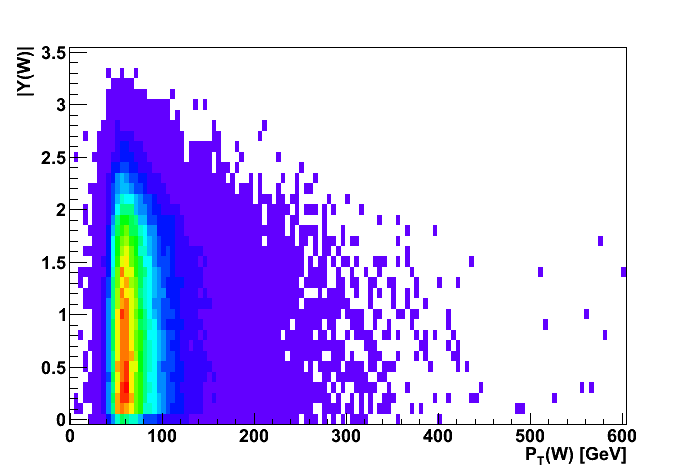
\includegraphics[width=0.47\textwidth]{fig/WPTvsY_mcreco50toinf}}\quad
\subfloat[\PtW]{
  \label{fig:wpol_genreco_ppt}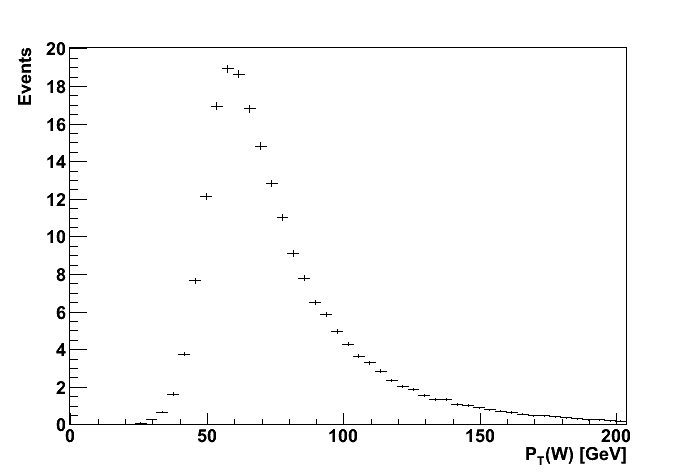
\includegraphics[width=0.47\textwidth]{fig/ptw_mcrecocut}}\quad
\caption{Generator level \PW phase space distributions after a
  reconstruction-level cut, $\PtW > \unit{50}{\GeV}$.}
\label{fig:wpol_genreco}
\end{figure}

\subsubsection{Closure Tests}
\label{sec:wpol_closure}
To ensure that the method is working correctly, several closure tests were
performed. Firstly, the generator-level helicity fractions within the phase
space of the reconstruction level \PW acceptance cuts are extracted. Essentially
the $\cos\thetastar$ distribution is plotted from a simulated sample of events
which have passed the reconstruction level \PtW cut. The distribution is fit,
once again using \eqn~\ref{eqn:wpol_helicity_fractions} and values of \f0, \fL and
\fR are extracted for both boson charges. This defines the baseline expectation
for the helicity fractions and is shown in Table~\ref{tbl:wpol_closure_tests}.

As a first closure test, the generator level \LP templates for each helicity
state are generated using the re-weighting method as described in
\sec~\ref{sec:wpol_reweighting} but excluding the acceptance correction. The
phase space again corresponds to the reconstruction levels cut on \PtW. The
binned maximum likelihood fit is then performed (see
\sec~\ref{sec:wpol_fitting}) and the helicity parameters obtained are shown
in Table~\ref{tbl:wpol_closure_tests}. The agreement with the aforementioned
generator level values is seen to be within the statistical error of the
simulated sample. Since at generator level, muon and electron channels should be
very similar, this was performed only in the muon channel.

Finally, a full reconstruction level closure test was performed in both electron
and muon channels and applying all of the analysis cuts listed in
\sec~\ref{sec:wpol_cutflow}. The results are also shown in
Table~\ref{tbl:wpol_closure_tests}. The muon channel is seen to recover the
``true'' helicity fractions to within the uncertainty of the analytical fit. The
electron channel, further complicated by \ac{QCD} contributions is seen to close
within the statistical error of the reconstruction-level fit. This corresponds
to \unit{100}{\invpicobarn} of simulated data.

\ctable[
cap=\PW Polarisation fit results for a number of closure tests,
caption=Fit results for the helicity fractions\, $f_{L}^{\pm}$ and $f_{R}^{\pm}$\,
for several closure tests of the re-weighting method described in
\sec~\ref{sec:wpol_reweighting}. The results of an analytical fit to the
$\cos\thetastar$ distribution\, having applied reconstruction level cuts on the
\PW boson\, are shown in the first column. The second column shows results from fits to the
\LP distribution at generator level in the muon channel. The final two columns
show the results of a full\, reconstruction-level closure test in both lepton
channels. The uncertainties have not been included for the reconstruction-level
muon fit since it is seen to close within the uncertanties of the analytical
fit.,
pos=h,
label=tbl:wpol_closure_tests,
doinside=\scriptsize
]{lcccc}{
}{\FL
            & Analytical Fit & Template Fit: Generator-Level & \Pgm Reconstruction-Level  & \Pe Reconstruction-Level \ML
$f_{L}^{-}$  & $0.5138 \pm 0.0032$     & 0.5149 & 0.5169 & $0.519\pm 0.038$\NN
$f_{R}^{-}$  & $0.2714 \pm 0.0027$     & 0.2708 & 0.2690 & $0.263\pm 0.040$\NN
$f_{L}^{+}$  & $0.5485 \pm 0.0026$     & 0.5506 & 0.5507 & $0.549\pm 0.048$\NN
$f_{R}^{+}$  & $0.2270 \pm 0.0021$     & 0.2286 & 0.2291 & $0.235\pm 0.019$\LL
}

\section{Analysis}
\subsection{Introduction}
To summarise what has already been said, the goal of this analysis is to extract
the helicity fractions (\fL, \fR and \f0) of the \PW boson and thus establish
the dominant left-handed polarisation effect present in theoretical predictions
at high \PtW. The \ffi coefficients determine the polar angle distribution
(\thetastar) via \eqn~\ref{eqn:wpol_helicity_fractions}. This distribution cannot
be reconstructed directly due to an ambiguity in the reconstruction of the \PW
boson rest frame. Instead the \LP variable, found to be highly correlated with
$\cos\thetastar$ in the limit of large \PtW is taken instead. Via a re-weighting
method, \LP distributions are constructed from \ac{MC} simulation
corresponding to 100\% left-handed, right-handed and longitudinally polarised
\PW bosons. These shapes may then be used in a fit to data in order to extract
the helicity fractions themselves.

It should be noted that the \ffi coefficients are expected to differ between
\PWp and \PWm. However, they are not expected to depend on the flavour of the
decay lepton. This is relevant to two aspects of this analysis. Firstly, as
shall be seen, the $\PW\longrightarrow\Ptau\Pgn$ decays where the \Ptau decays
to either and electron or a muon are included in the dataset. Secondly,
information from both electron and muon channels may be combined to constrain
the helicity fractions.

In order to perform this analysis, it is vital that a highly pure sample of
events containing \PW bosons is collected. Additional background contamination
must be accounted for in the fitting procedure, either by subtraction or by
incorporating an appropriate shape template. However this is handled, it will
inevitably introduce additional uncertainty into the fit. In the case of
subtraction, uncertainty on the shape and normalisation must be accounted for
and propagated into the uncertainties on the helicity fractions. Introducing an
appropriate template into the fit adds an additional parameter to account for
the relative normalisation as well as uncertainties stemming from the template
shape. This is particularly problematic in the case of \ac{QCD} multi-jet events
where the underlying processes are felt to be poorly understood. This
necessitates the use of a data-driven template which, as will be seen, brings an
additional set of complications.

\subsection{Backgrounds}
\label{sec:wpol_backgrounds}
It will be helpful to begin with a discussion of the backgrounds relevant to
this analysis. However, in order to understand the composition of the
backgrounds, the fundamental selection requirements should be stated. The
topology of interest are of course leptonic \PW decays, $\PW \longrightarrow
\Pl\Pgn$. In addition, the polarisation effect described in
\sec~\ref{sec:polarisation} is associated with \PW bosons produced with a
large transverse momentum. As was previously described, this serves to enhance
the quark-gluon interactions which lead to a strong left-handed
polarisation. Therefore, we find that the two most essential selection
requirements are as follows.
\begin{itemize}
\item A single isolated lepton typical of a \PW decay.
\item An event topology consistent with a large transverse momentum \PW. As will
  be seen in \sec~\ref{sec:wpol_wpt}, there is some freedom in the exact
  variables used to achieve this selection.
\end{itemize}
Taking only these two requirements, a considerable background will remain. As
will be shown, this can be largely eliminated via additional selection
criteria. The principal background sources may be categorised as follows.
\begin{itemize}
\item Drell-Yan production leading to a dilepton final state in which one of the
  leptons is missed due to limited acceptance, poor reconstruction or other
  detector effects such as electronics noise.
\item \ttbar production where $t\longrightarrow\Pbeauty\PW$ and the \PW then decays
  leptonically.
\item \ac{QCD} multi-jet events. In the muon channel, this can result from jet
  punch-through overlapping with a charged hadron or heavy-flavour
  decays. Electrons face a much higher background due primarily to photon
  conversions and overlap between charged hadrons and \Ppizero. The charged
  hadron leaves a track, whilst the \Ppizero decay leads to a shower of photons
  in the \ac{ECAL}.
\item For the electron channel only, there is an additional background from the
  conversion of promptly produced photons in \gammajets events.
\end{itemize}

\subsection{Leptons}
The first selection requirement is to choose events with a charged lepton
consistent with that of a \PW decay. Such events should, at a minimum, contain
at least one reconstructed electron or muon. Wherever possible, the lepton
selection criteria adopted were those used for the \PW cross section
analysis~\cite{cms_w_paper}. These requirements had been chosen to be as robust
as possible during the period of early data-taking at \ac{CMS}.

\subsubsection{Muons}
\label{sec:wpol_muons}
The requirements placed on the muon are as follows.
\begin{itemize}
\item The muon is required to be reconstructed as both a global muon and a
  tracker muon. This is to guard against either global muons mismatched with the
  tracker or noisy muon chambers in the case of tracker muons. For further
  information on muon identification, see \sec~\ref{sec:reco_muons}.
\item More than 10 hits in the tracker.
\item Bad muon fits are rejected by requiring $\chi^2 < 10$ on the global muon
  fit (tracker and muon chambers)
\item The transverse impact parameter of the muon with respect to the beam-spot
  is required to be $ < \unit{2}{\milli\metre}$. This is a fairly loose
  requirement but still rejects the majority of cosmic muons.
\item At least 1 hit is required in the pixels of the tracker in order to remove
  in-flight decays.
\item The tracker muon reconstruction must involve at least 2 muon
  stations. This suppresses punch-through and accidental matchings and ensures
  compatibility with the trigger.
\item The global muon reconstruction must involve at least 1 valid hit in the
  muon chambers; again to guard against decays in flight and punch-through.
\item A cut on the muon pseudorapidity $|\eta| < 2.1$ in order to ensure
  compatibility with the trigger requirements.
\item A cut on the \emph{combined isolation},
\begin{equation}
\label{eqn:wpol_mu_comb_iso}
  \CombIso = \frac{\sum_{\textrm{tracks}} p_T^{\textrm{track}} + \sum_{\textrm{dep}}
    E_T^{\textrm{em}} + \sum_{\textrm{dep}} E_T^{\textrm{had}}}{\Ptmu} < 0.1,
\end{equation}
where the sums run over the tracks in the tracker or the energy deposits in the
\ac{ECAL} and \ac{HCAL} within a cone of $\Delta R = \sqrt{(\Delta\eta)^2 +
  (\Delta\phi)^2} < 0.3$. A threshold of \unit{0.7}{\GeV} was placed on the
tracks contributing to the isolation sum.
\end{itemize}
Muons passing this set of selection criteria will be referred to as
\textbf{Tight}. Global muons failing one or more of these criteria will be
referred to as \textbf{Loose}.

\subsubsection{Electrons}
\label{sec:wpol_electronid}
The electron identification variables used are as described in
\sec~\ref{sec:reco_electron_id}. In order to achieve a strong suppression of
the \ac{QCD} multi-jet background, the decision was made to choose a tighter
working point than other \ac{CMS} analyses -- the 70\% efficiency working point
(see \sec~\ref{sec:wpol_electron_opt}). Electrons passing these criteria will
be referred to as \textbf{Tight}. For the purposes of vetoing dilepton events,
the 95\% efficiency cuts were used. These will be referred to as \textbf{Loose}
electrons.

In addition to the requirements of \sec~\ref{sec:reco_electron_id}, three independent
measurements of the charge are required to agree. These are measured as follows~\cite{wcharge_asymm2}:
\begin{itemize}
\item from the direction of curvature of the \ac{GSF} track;
\item from the track trajectory reconstructed using a Kalman filter and
\item from the azimuthal angle between the vector from the nominal interaction
  point to the \ac{ECAL} cluster and the vector joining the interaction point to
  the innermost hit of the \ac{GSF} track.
\end{itemize}
This requirement ensures that the charge misidentification rate is suitably low
for any resulting systematic uncertainty to be neglected (see
\sec~\ref{sec:wpol_syst_charge_misid}).

\subsection{Jets}
\label{sec:wpol_jets}
In order to reject events coming from \ttbar decays, which tend to have a large
jet multiplicity, an upper limit is placed on the number of jets in the
event. The jets are clustered using the \antikT algorithm from particle flow
reconstructed objects. A cone radius of 0.5 is used and an acceptance cut
$\modeta < 5$ is applied.

Additionally, cleaning is applied to events in which a jet overlaps with the
leading lepton. These cases are assumed to result from some misreconstruction
and thus should be excluded from the analysis. In the case of the electron, the
nature of the reconstruction algorithms introduces many such
overlaps. Consequently, jets found to lie within a cone $\Delta R < 0.3$ of the
highest \Pt lepton in the event are simply removed from consideration. In
contrast, for the muon channel, a much tighter cut can be afforded. Events are
completely vetoed from the selection if a single jet is found to lie within a
cone $\Delta R < 0.5$ of the muon.

\subsection{Kinematic Cuts}
\subsubsection{Transverse Momentum of the \PW Boson}
\label{sec:wpol_wpt}
The most vital kinematic cut to the analysis is the cut on the transverse
momentum of the \PW, \PtW. As has been discussed, requiring \PW bosons with a
large transverse momentum serves to enhance the polarisation effect described in
\sec~\ref{sec:polarisation}. It also ensures the correlation of \LP with
$\cos\thetastar$ and thus improves the measurement of the helicity
fractions. There are several means of reconstructing the \PtWv at \ac{CMS}. The
first, which was initially used for this analysis was the hadronic recoil of the
event. This is effectively the so-called missing hadronic energy of the
event, or \MHT,
% TODO Perhaps this should be moved somewhere else?
\begin{equation*}
\PtWvhad = - \sum_{j \in \textrm{jets}} \vec{j},
\end{equation*}
where the $j$ is taken to run over some subset of the jets in the event as
defined in \sec~\ref{sec:wpol_jets} with some minimum transverse momentum
requirement. The sum is taken to denote a vectorial sum. Since the \PW and the
jets must balance in the lab frame, this in principal provides an accurate
measurement of \PtWv. However, the reconstruction of the jets is difficult and
subject to uncertainties in the \ac{JES}. A higher resolution measurement can be
achieved by utilising instead the \METv (effectively the neutrino) and the
lepton in the event. This leads to the definition,
\begin{equation*}
  \PtWvlep = \Ptlv + \METv.
\end{equation*}
This provides a higher resolution measurement of \PtW, as can be seen in
\fig~\ref{fig:wpol_mht_res}. It is thus the variable adopted in this analysis.

\begin{figure}[h!]
  \centering
  \subfloat[]{\label{fig:wpol_mht_res1}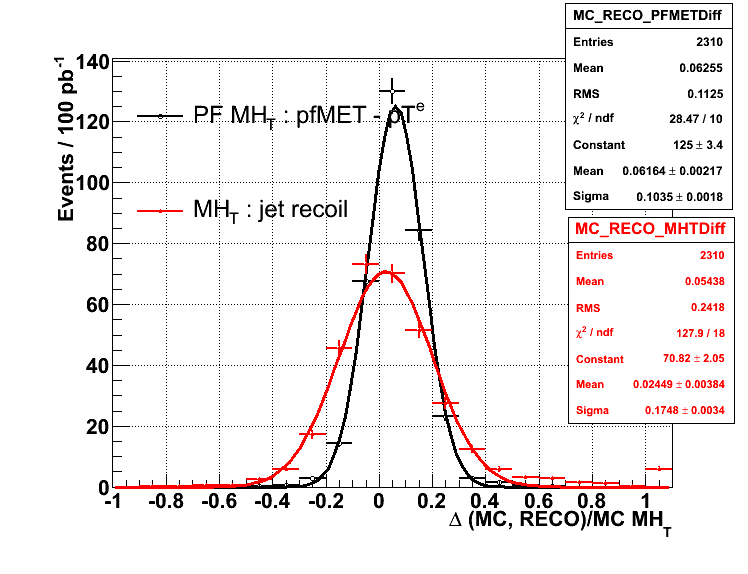
\includegraphics[width=0.4\textwidth]{fig/mht_res1.png}}\quad
  \subfloat[]{\label{fig:wpol_mht_res2}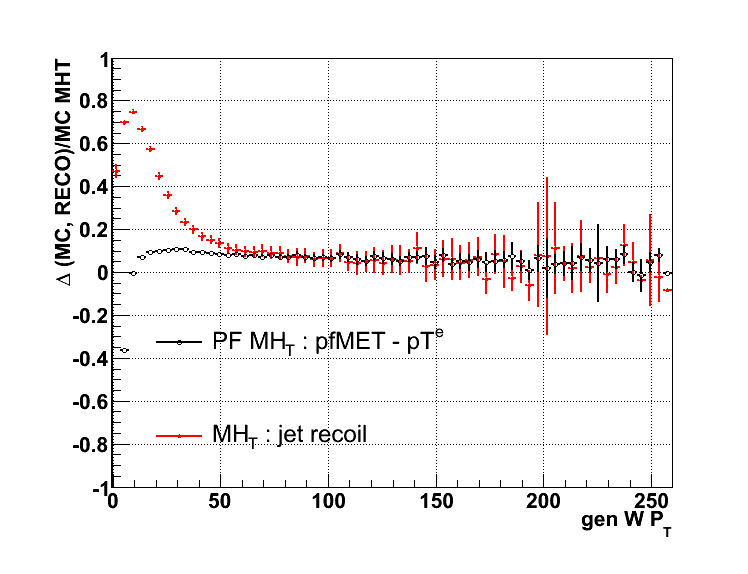
\includegraphics[width=0.4\textwidth]{fig/mht_res2.png}}
  \caption[Comparison of the helicity and background template
  shapes]{\fig~\ref{fig:wpol_mht_res1} shows the reconstruction-level \PtW
    resolution, $\left(\PtWgen - \PtWreco\right)/\PtWgen$, in the electron
    channel, using $\PtWvlep$ (black) and $\PtWvhad$
    (red). \fig~\ref{fig:wpol_mht_res2} shows the same resolutions as a
    function of \PtWgen.}
  \label{fig:wpol_mht_res}
\end{figure}

A second question, is then the choice of the minimum cut value to place on
\PtW. A tight cut on this quantity will reduce the efficiency of the analysis
selection, increase the statistical uncertainty on the measurement. In addition,
the simulated $\PW\longrightarrow\Pl\Pgn$ sample contains relatively few events
at high \PtW. With too tight a cut on \PtW, the statistical uncertainty on the
helicity templates will become significant. On the other hand, by placing a
tighter cut on \PtW, the difference between \fL and \fR -- the effect to be
measured -- will be enhanced. The correlation of \LP and $\cos\thetastar$ will
also increase.

The possibility of performing separate fits in bins of \PtW was also
considered. In the end the limitations mentioned above made this infeasible. For
a larger integrated luminosity, and given an adequate sample of simulated
events, such a measurement would be interesting. For this analysis, a moderate
cut, $\PtW > \unit{50}{\GeV}$, was adopted.

\subsubsection{Missing Transverse Energy}
In terms of rejecting backgrounds, tightening object definitions can only
achieve so much. Additional rejection power can be gained via additional
kinematic cuts on the event topology. As has already been stated, the \ac{QCD}
multi-jet background is the most problematic due to the fact that it is
relatively poorly modelled by \ac{MC} event generators. The simplest way to
reject such events is via a missing energy type cut. \ac{QCD} multi-jet events do
not typically contain a source of genuine missing energy. Experimentally
observed \MET from these events is typically due to jet mismeasurements,
detector noise or other problems with the event reconstruction. In addition, for
the high \PtW events of interest to this analysis, the missing energy component
(i.e. the neutrino) is often quite large. A relatively moderate cut on the \MET
is therefore able to reject the majority of such \ac{QCD} events.

However, a cut applied directly on the \MET introduces an additional
problem. Specifically, the \MET cut is effectively a selection on the momentum
of the neutrino in \PW events. This removes events, where for instance the
lepton has taken the majority of the momentum from the \PW and the neutrino is
thus very soft. This alters the shape of the \LP distribution. This will be
accounted for in the template shapes -- to be specific the left-handed and
right-handed templates will become more similar in shape. This increases their
correlation in the fit and is thus undesirable. More will be said of this in
relation to the electron measurement in \sec~\ref{sec:wpol_electron_opt}.

For this reason, it is desirable to cut on a variable that is not intrinsically
correlated with either the charged or neutral lepton momentum. The transverse
mass, \MT, is one such variable. Transverse mass is a variable chosen to
approximate the invariant mass of a particle by using only transverse
quantities. It is defined as follows:
\begin{equation*}
\MT = \sqrt{2\Ptl\MET\left(1 - \cos\Delta\phi\left(\Ptlv, \METv\right)\right)}.
\end{equation*}

The angular dependence (i.e. the $\cos\Delta\phi$ term) will effectively
compensate \PW decays in which either the charged or neutral lepton is soft
since these topologies will in general have a larger angular separation. Since a
momentum imbalance is exactly what is expected from the transverse polarisation
effect, the \MT cut avoids directly suppressing this effect.

Now considering the effect of the \MT cut on the background components, it is
not expected to strongly suppress either the \Zjets or \ttbar backgrounds since
these both contain real decays of a heavy particle. In the case of \ac{QCD}
multi-jet events, a balanced jet system has been badly reconstructed
such that one of the jets has been misidentified as a lepton. In general, the
fake \MET signature from these events will be small and thus rejected by the \MT
cut. In the case that the \MET component is larger due to a badly measured jet,
there are two possibilities.
\begin{itemize}
\item The mismeasurement has occurred on the jet that has been misidentified as a
  lepton. Since $\Delta\phi \sim 0$, the \MT cut should strongly suppress these
  events.
\item The mismeasurement has occurred on one of the other jets in the event. In
  this case, \MT may be large due to the large angular separation. Note however,
  that these events will in general be suppressed by the cut on \PtW
\end{itemize}

For the muon channel, it was found that a reasonably moderate cut $\MT >
\unit{30}{\GeV}$ was able to reduce the \ac{QCD} multi-jet background to
negligible levels. This was first demonstrated in simulation and then
cross-checked via comparison with genuine data. In the case of the electrons,
the background proved far more problematic. In the end, an $\MT >
\unit{50}{\GeV}$ cut was chosen for the sake of simplicity. For more detail on
the optimisation study in the electron channel, see
\sec~\ref{sec:wpol_electron_opt}.

\subsection{Selection Requirements}
\label{sec:wpol_cutflow}
Having discussed the selection requirements to be used in this analysis, the
actual cuts and cut values will now be presented. These are shown in
Table~\ref{tbl:wpol_cutflow}.

\ctable[
cap=Selection requirements for the \PW polarisation measurement,
caption=Selection requirements for the muon and electron channels in the \PW polarisation analysis,
pos=h,
label=tbl:wpol_cutflow,
doinside=\scriptsize
]{lcc}{
}{\FL
Selection             & Electron Channel & Muon Channel \ML
1 tight lepton        & $P_T^{\Pe} > \unit{25}{\GeV}$, $|\eta^{\Pe}| < 2.4$ & $P_T^{\Pgm} > \unit{15}{\GeV}$, $|\eta^{\Pgm}| < 2.1$ \ML
Veto 2nd loose electron or muon & $P_T^{\Pe} > \unit{15}{\GeV}$, $|\eta^{\Pe}| < 2.4$ & $P_T^{\Pgm} > \unit{10}{\GeV}$, $|\eta^{\Pgm}| < 2.1$\NN
 & $P_T^{\Pgm} > \unit{15}{\GeV}$ , $|\eta^{\Pgm}| < 2.1$ & $P_T^{\Pe} > \unit{15}{\GeV}$, $|\eta^{\Pe}| < 2.1$ \ML
$<4$ \ac{PF} jets & $\Pt > \unit{30}{\GeV}$, $|\eta| < 5.0$ & $\Pt > \unit{20}{\GeV}$, $|\eta| < 5.0$ \NN
Jet overlap veto & - & $\Delta R_{\textrm{min}}\left(\Pgm, \textrm{jet}\right) > 0.5$ \ML
\PW Boson \Pt & \multicolumn{2}{c}{$\PtW > \unit{50}{\GeV}$} \NN
\MT & $\MT > \unit{50}{\GeV}$ & $\MT > \unit{30}{\GeV}$ \LL
}

\subsection{Triggers}
\label{sec:wpol_triggers}
During the 2010 data taking period, the \ac{LHC} instantaneous luminosity
continued to evolve rapidly. The increased luminosity necessitated tightening of
the various object trigger requirements in order to maintain a suitable rate for
offline storage. This required careful selection of triggers for the analysis in
order to maintain efficiency with respect to the offline cuts.

For the muon channel, the triggers evolved quite slowly. In general, the cleaner
muon signature makes the triggers less susceptible to pile-up effects. The
triggers used were as follows:
\begin{equation*}
\begin{cases}
\texttt{HLT\_Mu9}          & \textrm{run} < 147146 \\
\texttt{HLT\_Mu15\_v1} & \textrm{run} \geq 147146.
\end{cases}
\end{equation*}
The naming scheme is that used by the \ac{HLT} at \ac{CMS}. The number in the
trigger name indicates the \Pt threshold applied to the lepton. The string
\texttt{vX}, differentiate different versions of the trigger key.

In contrast, the electron trigger thresholds evolved more rapidly,
\begin{equation*}
\begin{cases}
  \texttt{HLT\_Ele10\_LW\_L1R} & \textrm{run} < 140041 \\
  \texttt{HLT\_Ele15\_SW\_L1R} & 140041 \leq \textrm{run} < 143963 \\
  \texttt{HLT\_Ele15\_SW\_CaloEleId\_L1R} & 143963 \leq \textrm{run} < 146428 \\
  \texttt{HLT\_Ele17\_SW\_CaloEleId\_L1R} & 146428 \leq \textrm{run} < 147117 \\
  \texttt{HLT\_Ele17\_SW\_TightEleId\_L1R} & 147117 \leq \textrm{run} < 148819 \\
  \texttt{HLT\_Ele22\_SW\_TightEleId\_L1R\_v2} & \textrm{run} 148819 \leq \textrm{run} < 149181 \\
  \texttt{HLT\_Ele22\_SW\_TightEleId\_L1R\_v3} & \textrm{run} \geq 149181.
\end{cases}
\end{equation*}

Where \texttt{EleX} indicates an electron with $p_T > \unit{X}{\GeV}$. The
\texttt{LW} and \texttt{SW} stand for large window and small window
respectively~\cite{egamma_hlt_twiki}. Here, window refers to the electron pixel-matching window and thus
the large window cut is looser and intended to be used during start-up
conditions. All triggers include an \HoverE cut, $\HoverE < 0.15$. In addition,
those with \texttt{CaloEleId} or \texttt{TightEleId} impose additional electron
identification requirements. The former applies an additional \sigmaieta cut
(0.014 in the barrel and 0.032 in the endcaps). The latter applies constraints
on the angular matching variables between the track and the supercluster
($\deltaetain < 0.01$, $\deltaphiin < 0.08$) in addition to the \sigmaieta
requirement. These should be compared with the values in
Table~\ref{tbl:reco_electronid}.

\section{Validation in Simulation}
\subsubsection{Simulated Samples}
For each background component listed in \sec~\ref{sec:wpol_backgrounds}, an
appropriate simulated sample was used. In the case of the \Zjets, \ttbar and
\gammajets, the generator setup was as for the \Wjets sample -- the \ac{MADGRAPH}
matrix element generator interfaced to \pythia. In the case of the \ac{QCD}
background, a number of samples were used. In the case of the Muon channel, this
was a sample generated using \pythia and binned in terms of the transverse
momentum of the hard interaction, \pthat. This ensures adequate statistical
precision, even in the regions of high \pthat that will tend to pass the
analysis selection.

For the electrons, still larger statistics were required in order to study the
\ac{QCD} background properties. For these, \ac{QCD} samples were further
enriched towards the analysis level selection by selecting generator-level
electrons, photons, charged pions and charged kaons passing a set of loose
generator-level identification cuts approximating the isolation quantities and
\HoverE. This is referred to as the \textbf{EMEnriched} sample. An additional
sample is enriched by similar means with decays from \Pbottom and \Pstrange
hadrons. This is referred to as \textbf{BCtoE}. Both samples are again produced
in \pthat bins as for the unenriched sample. This generator level enrichment is
intended to reduce the costs in terms of time and disk space in processing a
much larger number of events, the majority of which will be rejected by basic
analysis cuts. An unfortunate side effect of this enrichement is that the
variables used in the filtering procedure may no longer be studied in their full
range. This is an impediment to certain background estimation studies which can
choose to invert certain lepton identification cuts.

Both data and \ac{MC} samples have been processed using \cmssw version 3.8.

\subsection{Signal and Background Expectations in Simulation}
\label{sec:wpol_yields}
The expected event yields across the relevant simulated samples are shown in
Tables~\ref{tbl:wpol_electron_yields} and \ref{tbl:wpol_muon_yields} for
electrons and muons respectively. The component marked \ac{QCD} denotes the
unenriched sample in the case of the muons and the sum of the
\textbf{EMEnriched} and \textbf{BCtoE} in the case of the electrons.

\ctable[
cap=\ac{MC} event yields in the electron channel of the \PW polarisation analysis,
caption=\ac{MC} event yields in the electron channel after each of the
selection requirements listed in Table~\ref{tbl:wpol_cutflow}. The yields shown
correspond to \unit{1}{\invpb} of integrated luminosity. A measure of the signal significance\, $S/B$\, is also given.,
pos=h,
label=tbl:wpol_electron_yields
]{lcccccc}{
}{\FL
Cut                    & W+Jets & QCD     & Z+Jets & $\gamma$+jets & $t\bar{t}$ & $S/B$ \ML
Trigger                & 6887.0 & 621013  & 804.4  & 1664.1        & 85.7       & 0.0   \NN
%$== 1$ loose electron & 5606.8 & 18299.7 & 369.7  & 627.3         & 24.4       & 0.3   \\ \hline
$N_e = 1$             & 2819.7 & 214.6   & 170.7  & 64.4          & 14.0       & 6.1   \NN
$N_{\mu} = 0$         & 2819.6 & 214.5   & 169.9  & 64.4          & 12.1       & 6.1   \NN
$< 4$ jets             & 2816.2 & 213.5   & 169.2  & 64.4          & 6.7        & 6.2   \ML
W boson $P_{T} > 50$ GeV & 182.2 & 17.2 & 28.4 & 15.9 & 5.0 & 2.7 \NN
$M_T > 50$ GeV           & 122.8 & 2.7  & 3.7  & 3.1  & 3.3 & 9.6 \LL
}
\ctable[
cap=Event yields in the muon channel of the \PW polarisation analysis,
caption=Simulated event yields in the muon channel after each of the
selection requirements listed in Table~\ref{tbl:wpol_cutflow}. The yields shown
correspond to \unit{1}{\invpb} of integrated luminosity. A measure of the signal significance\, $S/B$\, is also given.,
pos=h,
label=tbl:wpol_muon_yields
]{lccccc}{
}{\FL
Cut                                         & $W+$Jets   & QCD                  & $Z+$Jets  & $t\bar{t}$ & $S/B$ \ML
%Cross-section (pb)                         & 31314 NNLO & $8.76 \times 10^{8}$ & 3100 NNLO & 157.5 NLO  & -     \\\hline\hline
Trigger                                     & 7033       & 493887               & 909       & 28.1       & 0.01  \NN
$N_{\mu}=1$, $N_{e}=0$                      & 5086       & 27792                & 376       & 11.4       & 0.18  \NN
$< 4$ jets                                  & 5067       & 27740                & 368       & 5.5        & 0.18  \NN
$\Delta R_{\textrm{min}}(\mu$, jet$) < 0.5$ & 4979       & 26762                & 358       & 5.3        & 0.18  \NN
Second Muon Veto                            & 4973       & 26762                & 232       & 4.3        & 0.19  \ML
$\PtW > \unit{50}{\GeV}$                    & 264        & 21.3                 & 14.6      & 3.1        & 6.8   \NN
$\MT > \unit{30}{\GeV}$                    & 218        & 0.0                  & 5.4       & 2.0        & 26.0  \LL
}




\section{Fitting Procedure}
\label{sec:wpol_fitting}
In order to extract the helicity fractions in
\eqn~\ref{eqn:wpol_helicity_fractions}, a binned maximum likelihood fitting
procedure is performed. This takes \LP shape templates from the three \PW
helicity states, a number of data-driven or \ac{MC} estimated background
templates and extracts the most probably values of \fL, \fR and \f0 from the
data distribution. In order to test the procedure, this method is also applied
to \ac{MC} ``pseudodata'' to ensure that fitted helicity fractions match those
derived from the analytical fit (see \sec~\ref{sec:wpol_closure}) to within the
quoted errors. The fit itself is implemented in the \roofit software
framework~\cite{roofit_paper, roofit_web}, which assists in constructing an
appropriate likelihood function and performing the necessary minimisation using
the \minuit numerical optimisation code~\cite{minuit_paper}.

The number of signal events in a given histogram bin $i$ in terms of the
helicity fractions can be written as
\begin{equation}
\label{eqn:wpol_fit_signal}
S^j = \fL \hLj + \fR \hRj + (1-\fL-\fR)\hZj,
\end{equation}
where \hij are each binned helicity templates derived from the reweighting
method described in \sec~\ref{sec:wpol_reweighting}. The \f0
coefficient has been rewritten using the relation $\fL + \fR +\f0 = 1$ and thus
it is seen to be a two parameter fit.

\subsection{Electroweak Backgrounds}
As shown in \sec~\ref{sec:wpol_yields}, a non-negligible background component
is present in both channels arising from Drell-Yan and \ttbar production. These
can be referred to collectively as electroweak background contamination. For
these processes, the simulation is believed to be accurate enough to include
simulated \LP shape templates directly in the fit. In addition, the ratio of the
\Wjets vs electroweak background contributions is fixed assuming \ac{NLO}
cross-section
calculations~\cite{ellis_wp3jet,berger_wp4jet,heavy_quark,top_quark,drellyan}. The
combined electroweak background template is then incorporated into the fit as
follows:
\begin{equation*}
E^j = \fsig S^j + (1-\fsig) B^j,
\end{equation*}
where \fsig is the ratio of the simulated \Wjets yield to the total
simulated yield and $B^j$ is the combined \LP template for the \Zjets and \ttbar
backgrounds. It should be emphasised that the variable \fsig is not
free in the fit and thus does not introduce an additional degree of freedom.

\subsection{\acs{QCD} Background}
The previous formula is adequate for modelling the muon channel. For the
electron channel, it has already been shown that (see
Table~\ref{tbl:wpol_electron_yields}) \ac{QCD} multijet events as well as
\gammajets production provide a non-negligible additional contribution. To deal
with this, the formula is extended as follows:
\begin{equation*}
N^j = (1 - \fQCD) E^j + \fQCD Q^j,
\end{equation*}
where \fQCD is the ratio of the QCD multijet/\gammajets background
to the total event yield and $Q^j$ is a shape template derived via the procedure
described in \sec~\ref{sec:wpol_data_driven_bg}. Unfortunately, as has
already been stated, the simulation of QCD events is not yet reliable for direct
inclusion into the fit -- as for the electroweak backgrounds. From the
perspective of the fitting procedure, an important issue is that the relative
fraction \fQCD cannot be predicted from simulation. It is therefore
allowed to float freely in the fit. This procedure could be improved in future
by the inclusion of an independent measurement of the \ac{QCD} contamination,
for instance from a fit to the \MET shape. This would likely achieve better
separation of the \ac{QCD} component from the other backgrounds and thus a
tighter constraint on \fQCD.

\subsection{Fitting \fLmfR and \f0}
\label{sec:wpol_fit_fmfr}
For the final result, Equation~\ref{eqn:wpol_fit_signal} was modifed to fit
instead in terms of the parameters \fLmfR and \f0,
\begin{equation*}
S^j = \fLmfR \left (\hLj -\hRj\right) + \left(1-\f0\right)\left(\hLj +\hRj\right) +\f0\hZj.
\end{equation*}
This is appropriate given that \f0 and \fLmfR are related to the underlying
parameters \Azero and \Afour. It is also allows a more intuitive interpretation
in the context of the expected transverse polarisation effect. It should be
noted that since all helicity fractions must be non-negative,
$\fLmfR\leq\fLpfR$. Since $\fL +\fR + \f0 = 1$, it can be seen that $\fLmfR +
\f0 \leq 1$. This inequality defines the physical region of the parameter space.

\subsection{Combined Fit}
It has been noted that the helicity fractions are charge dependent but lepton
flavour independent. This suggests that the measurement may be refined by
simultaneously fitting both muon and electron channels. Due to the lower
efficiencies in the electron channel, this is not quite a doubling of the sample
size but should still significantly reduce the statistical error.

\section{Electron Channel}
\subsection{\ac{QCD} Background}
The principal difficulty faced by the electron channel over-and-above the muon
channel arises from the \ac{QCD} multijet background which, as has been seen,
remains even after tight kinematic and lepton identification cuts. This can be
discussed together with the promptly produced photon background (\gammajets)
which shares similar characteristics. These backgrounds enter the selection due
to some mismeasurement leading to a significant value of \PtW along with either
a real or fake lepton. They are highly problematic since their kinematics may
depend strongly on poorly understood \ac{QCD} processes -- namely the production,
hadronisation and measurement of hadronic jets. Because of this, currently
available simulation codes cannot be fully relied upon to correctly model the
kinematics of these events. This is particularly true in the case of the \LP
variable which is sensitive to both the leptonic and missing energy components
of the event.

To solve the problem presented by \ac{QCD}, two approaches were taken. The
first, described in \sec~\ref{sec:wpol_electron_opt} sought to suppress the
background as much as possible. This resulted in the tightened kinematic and
identification cuts that have already been detailed. The second focussed on
accurately modelling the remaining background component using a data-driven
procedure. This will be described in \sec~\ref{sec:wpol_data_driven_bg}. It
should be noted that these two strategies do not always complement each
other. It was possible to achieve larger supression of the \ac{QCD} background
whilst worsening the fit result. This occurs because the data-driven template
becomes ``flatter'' and the fit is less able to distinguish it from the helicity
templates in the fit.

\subsection{Kinematics}
Before continuing, it is useful to discuss the appearance of the \ac{QCD}
background in terms of the \LP variable. Consider the
measurement of \PtWv via the hadronic recoil in a balanced multi-jet event where
a single jet has been misreconstructed as an electron. In this case, the
hadronic recoil will tend to point along the axis of the fake electron. If the
hadronic recoil is then used as a measurement of \PtWv, it will be approximately
collinear with the \Ptlv of the fake electron and thus will yield a value of $\LP
\sim 1$. This can also be seen when the \PtW measurment is taken to be the
vector sum of \Ptlv and \METv. The fake electron will tend to be poorly
reconstructed and thus collinear with the source of fake \MET, again leading to
$\LP \sim 1$. A similar argument can be made in the case of \gammajets events
where now the photon is the source of both fake \MET and the fake lepton.


\subsection{Optimisation of Selection Requirements}
\label{sec:wpol_electron_opt}
A key challenge in the electron channel was posed by the significant background
from \ac{QCD} multijet events. \fig~\ref{fig:wpol_met_vs_mt_templates} shows
the effect of two possible kinematic cuts on the \LP shape for signal and
background events in simulation: $\MT > \unit{30}{\GeV}$ as used in the muon
channel, and $\MET > \unit{30}{\GeV}$. Clearly the \MET cut is more effective at
suppressing the \ac{QCD} background. However, the \MET cut also tends to remove
events with a soft neutrino, or alternatively a large \Pte. This is apparent in
the shape of the right-handed helicity template which has been ``cut away'' at
$\LP\sim 1$. The correlation of the left-handed and right-handed components is
increased, and the uncertainty from the fit is increased.

An optimisation study was undertaken to determine the optimal kinematic and
lepton identification cuts, as determined by the uncertainties from the template
fit. Some indication of the effect of the kinemtics cuts is given in
\fig~\ref{fig:wpol_ele_significance}. This shows the signal and background
yields as a function of varying \MET and \MT cuts applied after all other cuts
listed in Table~\ref{tbl:wpol_cutflow}. The background in this case is the sum
of the processes listed in \sec~\ref{sec:wpol_backgrounds}. Also shown are
two possible measures of the signal significance, again with varying \MET and
\MT cuts. As can be seen, the \MET cut is significantly more effective at
supressing the background. However, this comes at the cost of considerably
reduced signal statistics. The significance plots could also be construed to
support a \MET cut over an \MT but of course, since the final results are
extracted from a template fit, the \LP shape must also be considered.

This point is further reinforced in \fig~\ref{fig:wpol_met_mt_fqcd}. Here the
$x$ and $y$ axes denote cut values of \MET and \MT. For each point on the plot,
the fraction of the total event yield due to \ac{QCD} mutlijet production is
plotted for those events surviving a combined cut on the \MET and \MT.

\fig~\ref{fig:wpol_wp80_vs_wp70} compares the \LP shape in signal and
background events using two different electron ID working points. The 70\%
efficiency working point is seen to reject considerably more of the \ac{QCD}
background. This motivated the use of the tighter electron ID.

\begin{figure}[h!]
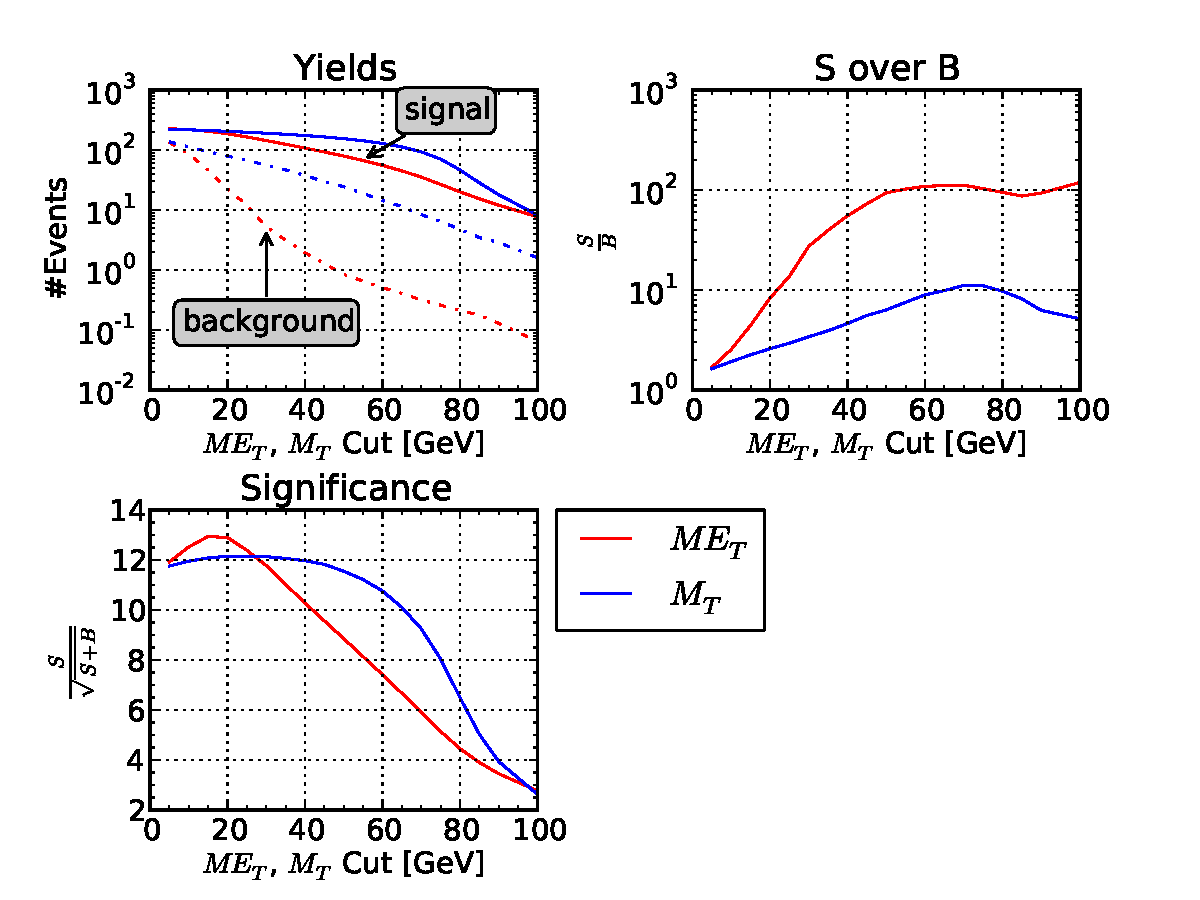
\includegraphics[width=0.8\textwidth]{fig/ewpol_significance}
\caption[Plots illustrating the signal significance in the electron channel with
respect to varying cuts on \MET and \MT.]{Plots illustrating the signal
  significance in the electron channel with respect to varying cuts on \MET and
  \MT. All other selection requirements have been applied. Top-left shows the
  dependence of the signal (solid lines) and background yields (dotted lines)
  for varying \MET (red) and \MT (blue) cuts. Similarly top-right shows the
  signal significance using the metric $S/B$ and bottom-left using the metric
  $S/\sqrt{S+B}$.}
\label{fig:wpol_ele_significance}
\end{figure}

\begin{figure}[h!]
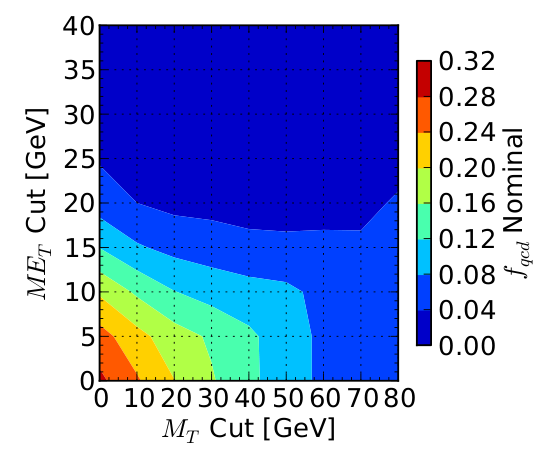
\includegraphics[width=0.5\textwidth]{fig/qcd_nom}
\caption{Two dimensional plot showing the dependence of \fQCD on a combined \MET
  and \MT cut in the electron channel as observed in simulation. \fQCD
  represents the fraction of the total event yield originating from \ac{QCD}
  multijet events. All other selection requirements have been applied. }
\label{fig:wpol_met_mt_fqcd}
\end{figure}

\begin{figure}[h!]
\centering
\subfloat[]{\label{fig:wpol_met_vs_mt_templates_met}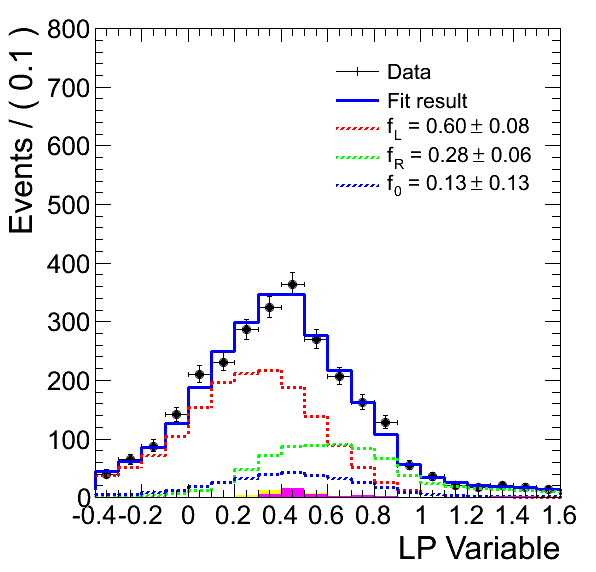
\includegraphics[width=0.4\textwidth]{fig/e_lp_fit_met30}}\quad
\subfloat[]{\label{fig:wpol_met_vs_mt_templates_mt}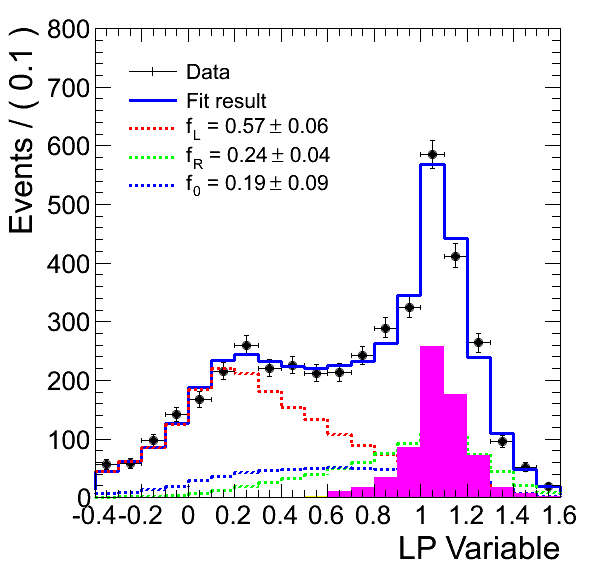
\includegraphics[width=0.4\textwidth]{fig/e_lp_fit_mt30}}
\caption[Comparison of the helicity and background template shapes]{Comparison
  of the helicity and background template shapes after
  \subref{fig:wpol_met_vs_mt_templates_met} $\MET > \unit{30}{\GeV}$ or
  alternatively \subref{fig:wpol_met_vs_mt_templates_mt} $M_T >
  \unit{30}{\GeV}$. }
\label{fig:wpol_met_vs_mt_templates}
\end{figure}

\begin{figure}[h!]
\centering
\subfloat[]{\label{fig:wpol_wp80}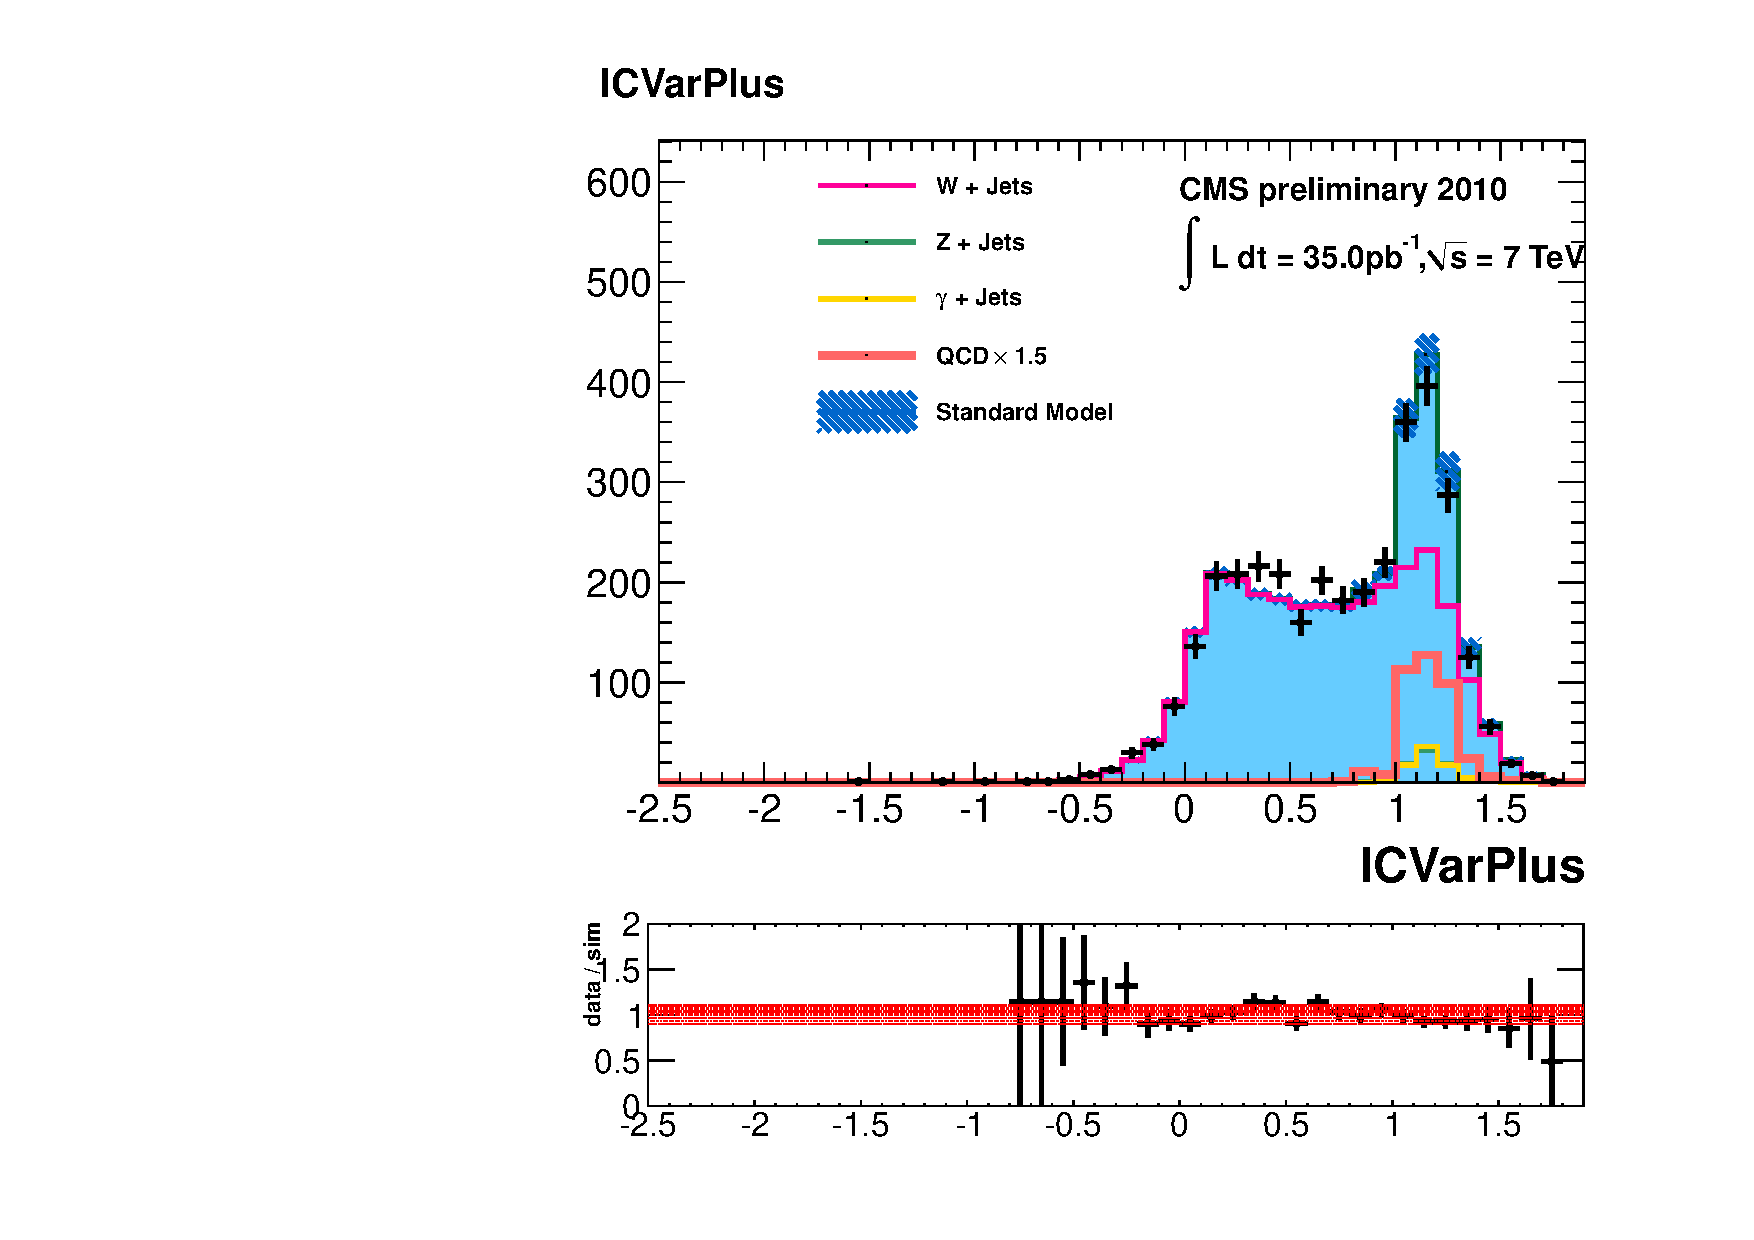
\includegraphics[width=0.4\textwidth]{fig/ICVarPlusMT50_WP80}}\quad
\subfloat[]{\label{fig:wpol_wp70}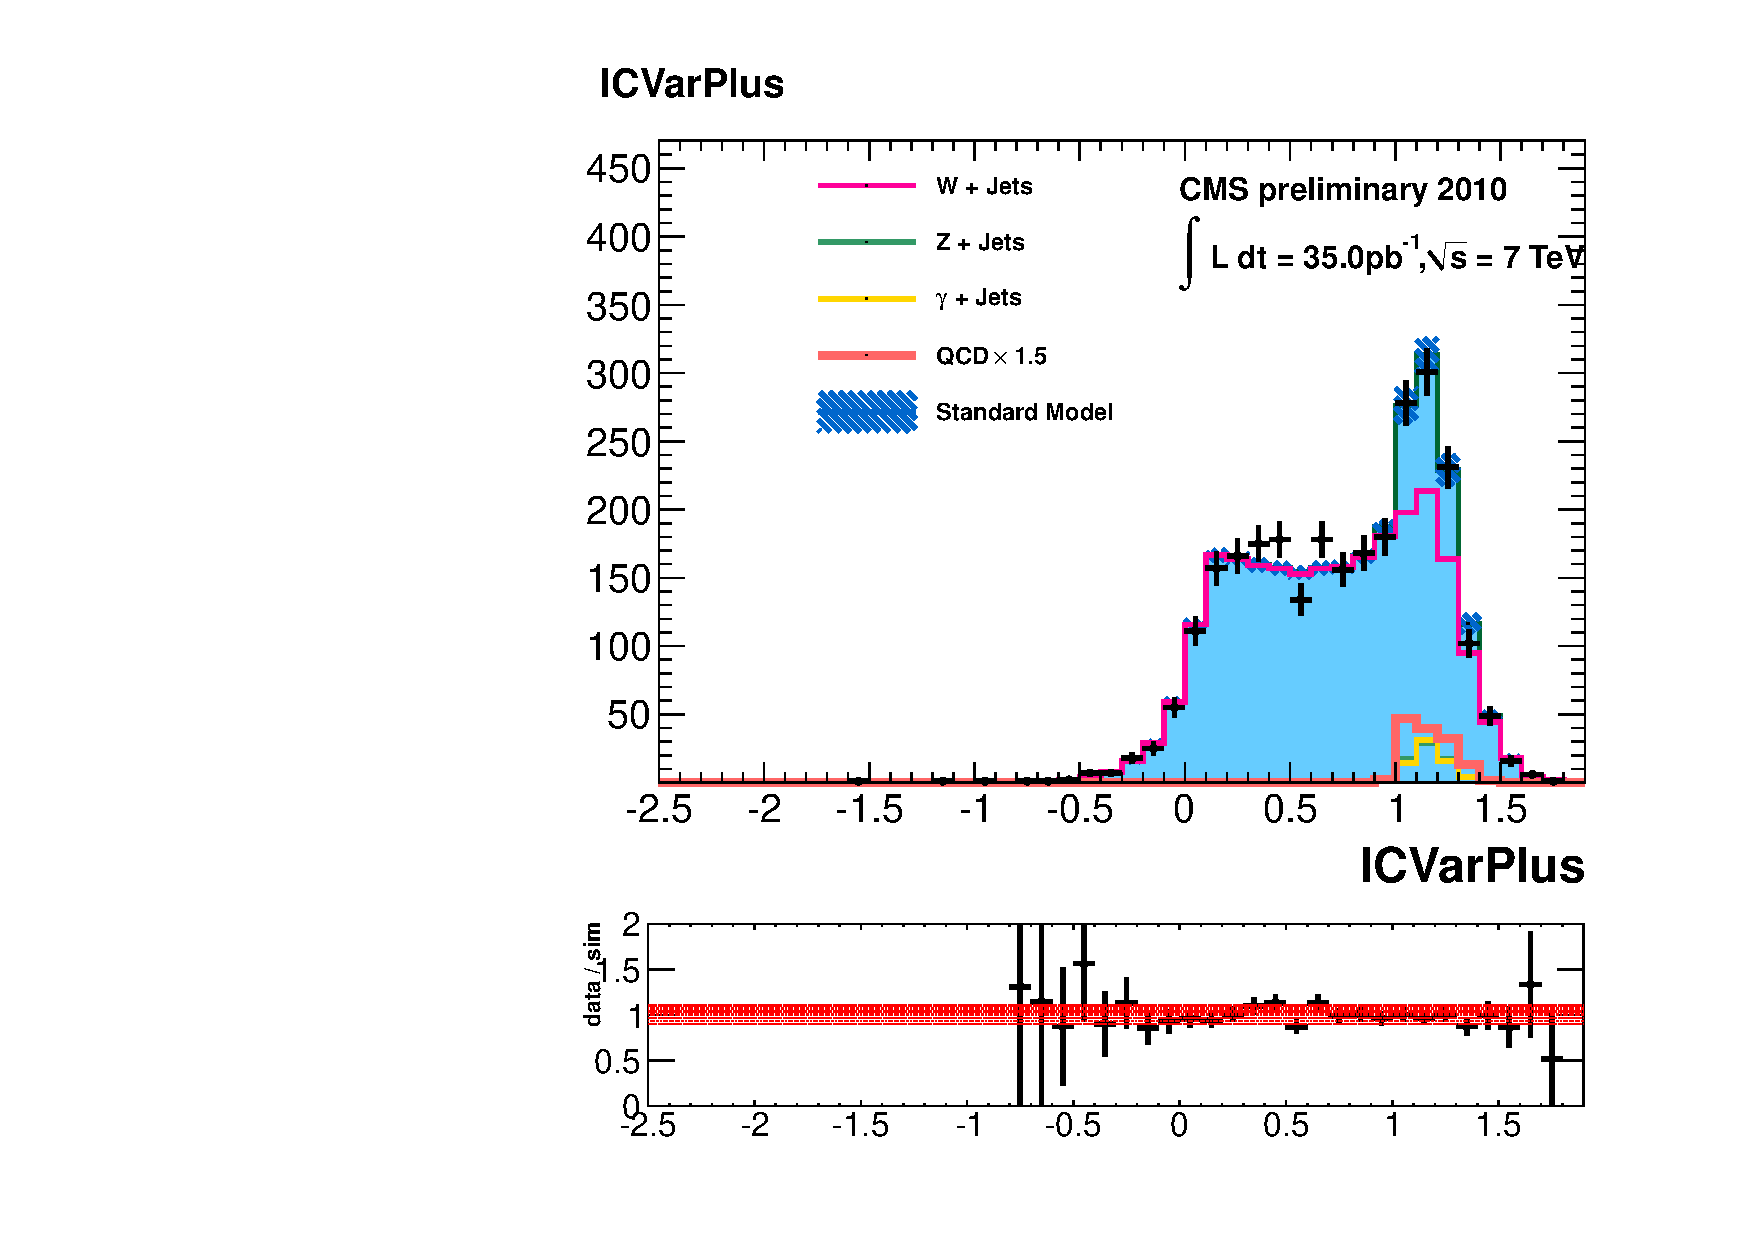
\includegraphics[width=0.4\textwidth]{fig/ICVarPlusMT50_WP70}}
\caption[]{The shape of the \LP distribution in data and \ac{MC} for two electron
  ID working points: \subref{fig:wpol_wp80} the 80\% efficiency selection and
  \subref{fig:wpol_wp70} the 70\% efficiency selection.}
\label{fig:wpol_wp80_vs_wp70}
\end{figure}

\subsection{Data-Driven Background Template}
\label{sec:wpol_data_driven_bg}
To produce a reliable \LP shape template for \ac{QCD} and \gammajets events, a
data-driven procedure is needed which will yield a control sample enriched with
\ac{QCD} events resembling those entering the selected sample. Such a control
sample is often constructed by anti-selection. Consider the variables used for
the analysis selection as a multi-dimensional space in which the cut values
enclose some region which contains the selected sample -- the ``selected''
region. The anti-selected sample is then constructed by inverting the cuts on a
subset of these variables. The region in this space selected by the inverted
cuts is then referred to as the ``anti-selected'' region. Since the majority of
the cuts are common to both selected and anti-selected samples, it can be
expected that they will share similar kinematic properties.

A variable suitable for inversion in this procedure must satisfy two
criteria. Firstly, it must provide separation power between the \ac{QCD}
background that we wish to model and the other electroweak signal and background
events. Secondly, the \LP shape must be similar between the selected and
anti-selected regions. Put another way, the inverted variable must be
uncorrelated with \LP. An additional requirement is that the anti-selected
region (which may be the result of several inverted variables) contain adequate
statistics for construction of a shape template.

As the analysis was developed, a variety of anti-selection regions were tested
using \ac{MC} samples. One practical problem is that adequate statistics for
these tests could only be obtained by using the enriched \ac{QCD} sample. Since
this sample has an implicit cut on the electron isolation, it was not possible
to study the inversion of this variable. Many combinations of the electron
identification variables were tried. Many proved to be correlated with \LP via
either the leptonic or missing energy component.

In the end, the best compromise was achieved by inverting the track-supercluster
matching parameters, \deltaetain and \deltaphiin, on the leading electron. A
comparison of the selected and anti-selected shapes derived from this procedure
is shown in \fig~\ref{fig:wpol_ele_sel_antisel} before and after the \MT
cut. The \LP shape for \ac{QCD} background is not believed to have a charge
dependence and thus the shapes for positive and negative charge are combined
into a single template to mimimize statistical uncertainty.

\begin{figure}[h!]
\centering
\subfloat[]{\label{fig:wpol_antiselected1}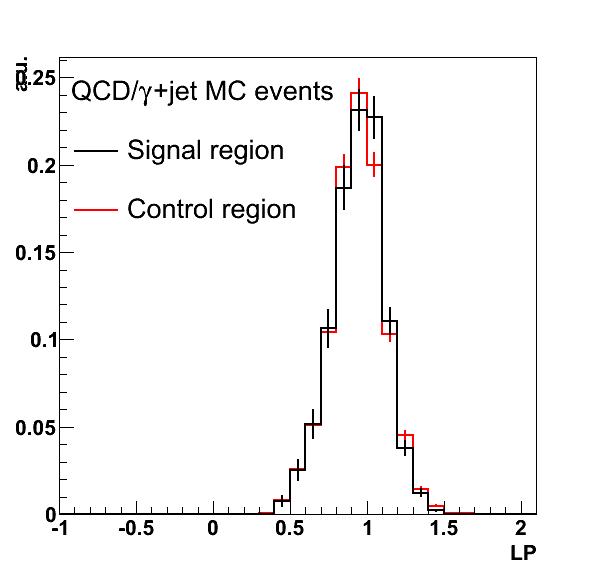
\includegraphics[width=0.4\textwidth]{fig/antiselected1}}\quad
\subfloat[]{\label{fig:wpol_antiselected2}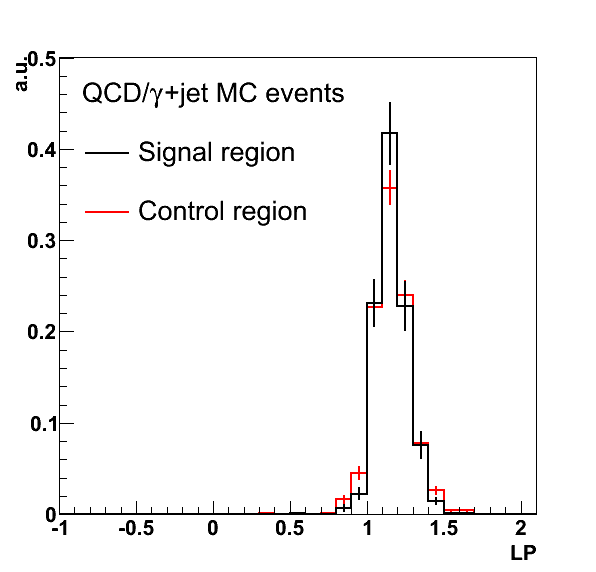
\includegraphics[width=0.4\textwidth]{fig/antiselected2}}
\caption[]{The \LP variable shown for selected (black) and anti-selected (red)
  simulated \ac{QCD} events after \subref{fig:wpol_antiselected1} $\PtW >
  \unit{50}{\GeV}$ and \subref{fig:wpol_antiselected2} $\MT > \unit{50}{\GeV}$}
\label{fig:wpol_ele_sel_antisel}
\end{figure}

\section{Systematic Uncertainties}
\label{sec:wpol_systematics}
The template reweighting method necessary for the extraction of the helicity
fractions introduces an inescapable dependence on \ac{MC} simulation. One of
the challenges for this analysis is to ensure that any potential mismodelling
within the simulation which might affect the construction of the \LP templates
is properly accounted for and included in the systematic uncertainty on the
final result. Two kinds of uncertainty will be considered: those stemming from
experimental effects, and those due to uncertainties in the theoretical input to
the measurement.

\subsection{Experimental Uncertainties}
In considering the potential sources of systematic error, it is helpful to think
first in terms of the construction of the \LP variable. This involves two
detector level quantities: the missing transverse energy \METv and the
transverse momentum of the charged lepton \Ptlv. The first quantity is derived
from the particle flow algorithm, as discussed in \sec~\ref{sec:reco_pf}. The
leading source of uncertainty is due to the callibration of the jet energy
scale.

\subsubsection{\acl{JES}}
\label{sec:wpol_syst_jec}
The \ac{JES} is discussed in \sec~\ref{sec:reco_jets}. The uncertainty on its
calibration has been thoroughly studied and is parameterised as a function of
jet \Pt and $\eta$. In the case of a global miscalibration of this measurement,
jet energy measurements in data would be pushed upwards or downwards with
respect to the values predicted by simulation. If one imagines a perfectly
balanced dijet system in the centre of the detector, the resulting effect on the
\METv will of course be cancelled. However, this will rarely be the case. In
particular, in the case of \Wjets production, the hadronic system will be
recoiling against the \PW. For relatively high transverse momentum \PW bosons,
the \METv is very likely to point away from the recoiling jets. This suggests
that the effect of an upward or downard shift in the \ac{JES} is likely to have
an opposite effect on the \METv scale and be highly correlated between
events. In other words, a shift in the \ac{JES} will, to first order,
lead to an opposite shift in the \MET distribution. Of course there are angular
effects of an adjustment to the \ac{JES}, which were fully modelled in
simulation. For now a heuristic argument will suffice to understand the most
striking effects.

The dominant effect of the \ac{JES} on the fitted helicity fractions is due to
the change in the \LP shape. Of course, the effect will also affect the cuts on
\PtW and \MT and this has also been modelled in simulation. The shift in the
\MET due to the \ac{JES} will correspond directly to a shift in the calculated
\LP. For an upwards shift in the \ac{JES}, the \MET will tend to shift downwards
and thus to larger values of \LP. Conversely, for a downward shift in the
\ac{JES}, the \MET scale will increase and therefore \LP will shift to smaller
values. This very approximate argument is born out in the full modelling in
simulation. This is illustrated in \fig~\ref{fig:wpol_mujecunc} showing the
fractional change of the \LP distribution in the muon channel for upward and
downward shifts in the \ac{JES}. Clearly, the effect is quite large and most
severe towards the edges of the \LP distribution (i.e. $\LP < 0$ and $\LP >
1$). There are two reasons for this. Firstly, that in these regions the \LP
distribution is rising or falling rapidly. Bin to bin migration will thus yield
larger changes. Secondly, the change in the value of \LP for a single event in
response to a change in the \ac{JES} is expected to be linear in \LP to first
order.

The \ac{JES} is the dominant source of systematic uncertainty in the muon
channel and very significant in the electron channel. The effect can be
mitigated somewhat however by the observation that a restricted fit range will
insulate the measurement from the most severe changes to the \LP shape. Whilst
the edges of the \LP distribution are the source of the largest \ac{JES}
uncertainty, they also tend to contribute a lot to the fit. Reducing the fit
range too drastically may remove too much information from the fit, increasing
the statistical error and negating any benefits from the reduced systematic
uncertainty. An optimisation study was undertaken in both lepton channels and
for both charges to choose an optimal fit range.  The quadratic sum of the
statistical and systematic errors was calculated for a selection of possible fit
ranges. It was determined that a fit range of $[0,1.3]$ was an appropriate
choice for both channels and both charges.

\begin{figure}[h!]
\centering
\subfloat[$\LP(\APmuon)$]{\label{fig:wpol_mujecunc_p}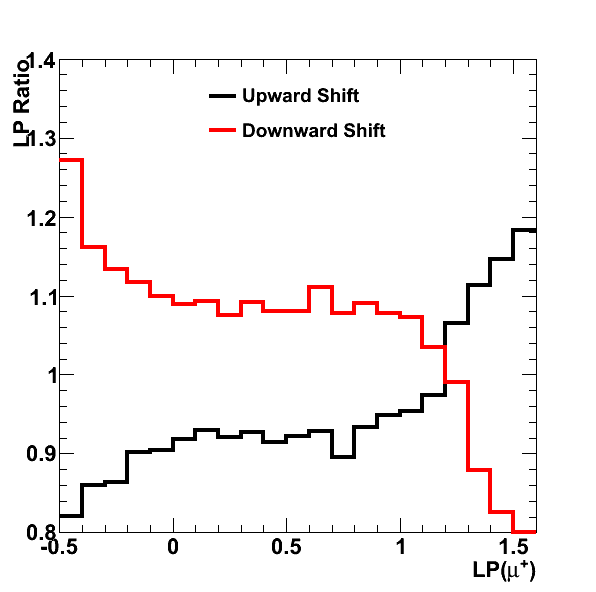
\includegraphics[width=0.4\textwidth]{fig/pLP_jecuncratios}}\quad
\subfloat[$\LP(\Pmuon)$]{\label{fig:wpol_mujecunc_m}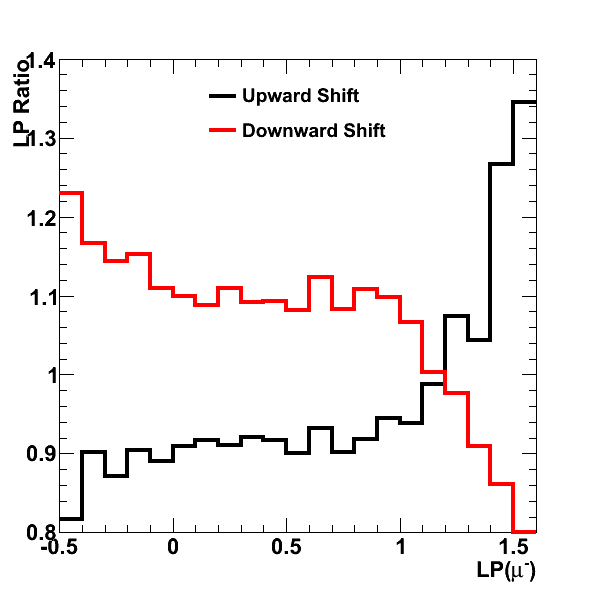
\includegraphics[width=0.4\textwidth]{fig/mLP_jecuncratios}}
\caption{Relative change of the muon \LP distribution due to the effect of the
  \ac{JES} uncertainty. The black line corresponds to an upward shift
  with respect to the original distribution, and the red line a downward shift.}
\label{fig:wpol_mujecunc}
\end{figure}

The \ac{JES} uncertainty follows the standard prescription for \ac{CMS}
analyses. Firstly, the unclustered component of the missing energy is calculated as,
\begin{equation*}
\vec{E}^{\textrm{unclustered}}_T = -\METv + \Ptlv + \sum_i \vec{p}_T^{\textrm{jet},i},
\end{equation*}
where the index $i$ runs over all jets with $\Pt > \unit{10}{\GeV}$ in the event
as reconstructed by the particle flow algorithm. The unclustered energy is then
scaled either up or down within its uncertainty -- taken to be
5\%~\cite{jet_energy_pas}. \METv is then recalculated from this displaced
unclustered energy,
\begin{equation*}
\METv \longrightarrow -\vec{E}^{\textrm{unclustered}}_T - \Ptlv - \sum_i (1 \pm  u(p_T, \eta)) \times \vec{p}_T^{\textrm{jet},i},
\end{equation*}
where $u(p_T, \eta)$ is a map specifying the relative uncertainty on the jet
energy scale as a function of jet transverse momentum and pseudorapidity. The
scale applied to the jet momenta will be in the same direction as that of the
unclustered energy. When calculating the effect on the results, this displaced
value is then used in place of the \METv and all \METv derived quantities. The
end product of this are two modified \LP shapes corresponding to upward and
downward fluctuations in the \ac{JES}. Since the shifted \METv has been
applied consistently throughout the analysis, the smaller effects on \PtW and
\MT are also included.

The value of the \ac{JES} systematic is determined in simulation by
fitting the unaltered template (with no \ac{JES} adjustment) to
pseudodata resulting from the upward and downward shifts. Taking the difference
of the upward and downward scaled cases with respect to the unaltered yields
asymmetric uncertainties on each of the helicity fractions. The final systematic
uncertainty is then taken to be largest of the two errors.

\subsubsection{\MET Resolution}
In addition to the modelling of the \ac{JES}, another possible source of
mismeasurement stems from the resolution effects included in the simulation of
the detector. The resolution predicted by the \ac{MC} is known to
considerably underestimate that observed in the
data~\cite{cms_met_paper,cms_met_pas}. To account for this, additional
``smearing'' was applied to the missing transverse energy in simulation. The
difference between this ``increased resolution'' case and the nominal conditions
in simulation is then taken as an additional source of systematic error.

As the first step of the procedure, the resolution on \PtW is extracted from the
simulation in bins of the generator level \PtW quantity. For simulated \Wjets
events with a reconstructed electron or muon and a matching generator level
particle or a generator level \Ptau, the following quantity is calculated,
\begin{equation*}
\Delta\PtW = \frac{\PtWgen - \PtWreco}{\PtWgen},
\end{equation*}
where \PtWreco and \PtWgen refer to the reconstruction and generator level \PW
transverse momentum respectively. This is the relative difference between the
reconstruction and generator level \PtW. This distribution is then divided into
bins of generator level \PtW. Each bin is fit with a Gaussian distribution in
order to extract the resolution, $\sigma_{\PW}$ as a function of \PtW. This is
the \PtW resolution as modelled by the detector simulation.

The simulated sample is then used again, this time ``smearing'' the
reconstruction level \PtW quantity such that the resolution is increased by
10\%. This is the value measured in~\cite{cms_met_paper}. These are fit with the
``unsmeared'' templates and the difference with respect to the nominal is
assigned as a systematic. A less conservative estimate could be obtained by
correcting the resolution in simulation to match the data and then assigning the
uncertainty of the correction as the systematic uncertainty. However, since this
uncertainty has not been precisely estimated, the simpler, more conservative
estimate was used.

\subsubsection{Lepton Momentum Scale}
The second contribution to the \LP shape uncertainty comes from the lepton
momentum measurement. The character and magnitude of the uncertainty is quite
different for the electron and muon channels.

The muon momentum scale uncertainty due to material and B-field uncertainties
has been shown to be small. However, a charge asymmetric \Pt bias might appear
via ``$\chi^2$ invariant modes''~\cite[section
2.4]{matthias_edelhoff_thesis}. By calculating the difference in the \PZ mass
between events with a positively and negatively charged leading muon (in terms
of \Pt), the size of this effect can be judged. No significant effect is
observed in data. The errors on this measurement are used to place an upper
bound on such an effect. The effect is found to be less than 1\% at a \Ptmu of
\unit{100}{\GeV} and this is taken as a systematic uncertainty. This is
propagated to the helicity fractions by adjusting the \Ptmu in simulation by
$\pm 1\%$ and taking the difference from the unaltered case.

Uncertainty on the electron momentum scale is dominated by the effect of the
\ac{ECAL} transparency changes described in
\sec~\ref{sec:expt_laser_monitoring}. Corrections to account for this effect
were derived for the \PW charge asymmetry
measurement~\cite{w_charge_asymmetry}. The detector is divided into 6 bins in
$\eta$. The \Zee mass distribution in data is then divided into $6 + ^6C_2$
categories corresponding to cases where a \PZ is reconstructed from electrons in
$\eta$ bins $i$ and $j$.  For each category a mass template is derived from
simulation. A simultaneous fit is then performed over the 21 categories, where
each template is scaled by the factor $1/\sqrt{s_is_j}$ and smeared by a
resolution term $\sqrt{\sigma_i^2 + \sigma_j^2}$. This results in a set of 6
scale terms, $s_i$ and 6 resolution terms, $\sigma_i$. These are shown in
\fig~\ref{fig:wpol_ecal_transp_corr}.  The scale terms should be applied to
data, whilst the resolution should be applied in simulation.

\begin{figure}[h!]
  \centering
  \subfloat[Scale corrections, $s_i$]{\label{fig:wpol_ecal_transp_scale}\includegraphics[width=0.45\textwidth]{fig/ecal_transp_scale}}\quad
  \subfloat[Resolution corrections, $\sigma_i$]{\label{fig:wpol_ecal_transp_sigma}\includegraphics[width=0.45\textwidth]{fig/ecal_transp_sigma}}\quad
  \caption{\ac{ECAL} transparency correction factors as a function of
    pseudorapidity. These are determined from a fit to the \PZ mass distribution
    as described in the text~\cite{w_charge_asymmetry_an}.}
\label{fig:wpol_ecal_transp_corr}
\end{figure}

The scale corrections have been applied in data. An conservative 50\%
uncertainty was taken on the value of the correction factors. The lepton
momentum in simulation is then adjusted by $\pm 50\%$ of the correction factor
and the resulting change in the fit results with respect to the unaltered case
is taken as a systematic uncertainty. This is equivalent to correcting the data
by either 50\% of 150\% of the correction factors.

The effect of the resolution corrections on the fit results was also judged by
applying them in \ac{MC}. The resulting change was found to be negligible,
and thus these factors were not applied in data.

Since the method described above performs a global correction, the mean of the
lepton momentum distribution is corrected, but the wdith will also be
increased. By making use of the continuous measurements provided by the laser
monitoring system, this could be significantly improved. These corrections were
not fully validated on the timescale of the analysis. As a cross-check, the
analysis was also performed using a preliminary version of the continuous
corrections. The results were found to be fully consistent with those obtained
using the continuous corrections.

\subsubsection{Electron \ac{QCD} Background Estimation}
\label{sec:wpol_syst_ele_bgest}
As discussed in \sec~\ref{sec:wpol_data_driven_bg}, the template used to fit
the \ac{QCD} multijet background component in the electron channel has been
derived from a data-driven method. As has been shown, the simulation shows a
very similar \LP shape between the selected and anti-selected samples. However,
the small differences that can be seen coupled with the very limited statistics
available in \ac{MC}, necessitate the inclusion of an additional systematic
uncertainty.

The first systematic represents the degree, as can be judged from the enriched
\ac{QCD} \ac{MC} sample, that the anti-selected template mismodels the \LP shape
of the \ac{QCD} events in the selected region. In other words, the bias
introduced by any correlation between \LP and the track-supercluster matching
variables, as far as can be judged in simulation. This is evaluated by
performing 500 toy experiments. For each toy experiment, the \ac{MC} pseudodata
is first fitted using the \ac{QCD} template taken directly from the selected
region. This represents the case, where the \ac{QCD} has been modelled perfectly
by the template. Then the pseudodata is refit using the anti-selected template
and including contamination from the other simulated samples. The ensemble
distributions of the fit parameters are then compared between the ``true'' case
using the actual \ac{QCD} \ac{MC} shape and the ``data-driven'' case using the
anti-selected template. The difference in the means of the ensemble
distributions for the parameters \f0 and \fLmfR is then taken as a systematic
uncertainty. This is performed separately for both charges.

The second systematic represents the uncertainty introduced by the very limited
statistics available in the simulated \ac{QCD}/\gammajets samples. The bins of
the \ac{MC} anti-selected template were each fluctuated about their mean
values and within their statistical uncertainties. This procedure is performed
for the whole template 500 times, to give 500 ``re-diced'' templates. Each
re-diced template is then fitted along with the standard signal and electroweak
background templates to the pseudodata. The ensemble distributions of \f0 and
\fLmfR are then plotted and the \ac{RMS} widths taken to be the systematic
uncertainty due to limited statistics in the \ac{QCD} template.

\subsubsection{Vertex Multiplicity}
The vertex multiplicity changed rapidly during data taking. Due to the long
lead-time in the production of simulated samples, it was not feasible to produce
samples with vertex multiplicity distributions exactly matching those present in
data. In order to correct the simulation to match the data, the simulated and
observed vertex distributions were compared. The simulated samples were then
reweighted to account for this difference. A systematic uncertainty is assigned
by allowing the reweighting factors to vary within their statistical
uncertainties. The uncertainty was tested in the muon channel and found to be
negligible.

\subsubsection{Charge Misidentification}
\label{sec:wpol_syst_charge_misid}
Misidentification of the reconstructed lepton charge causes events to migrate
between the \PWp and \PWm samples. Since the templates are different for each
charge, this could bias the results of the fit. Any possible effect in the muons
is known to be negligible. For the electrons, the three charge requirement
brings the charge misidentification rate below 1\%. At this level, the
systematic related to charge misidentification is negligible in comparison to
the other sources of uncertainty.


\subsection{Theoretical Uncertainties}
In addition to the experimental uncertainties, the method relies upon
theoretical assumptions which can alter the extracted helicity fractions.

\subsubsection{\Ai Dependence}
Measurement of \f0 and \fLmfR will depend on the values of the other \Ai
coefficients (besides \Azero and \Afour). This was tested in simulation by
varying each parameter \Ai by 10\% of its value -- an uncertainty derived from
comparison of \ac{LO} and \ac{NLO} calculations by the Blackhat
collaboration. The value of \fLmfR is found to have a very small dependence on
the values of the other \Ai.

\subsubsection{\aclp{PDF}}
\label{sec:wpol_syst_pdf}
This analysis used a \Wjets \ac{MC} sample, generated using the \cteqsixlone
\ac{PDF} set~\cite{cteq6l1}. This is a set of 41 \ac{PDF} distributions. All
results in this analysis are calculated using the best fit value of this set. To
determine the uncertainty associated with this assumption, each alternative
\ac{PDF} from the set is selected and modelled in the \ac{MC} via a
reweighting procedure. From this, 40 separate \LP distributions are derived
representing pseudodata assuming an alternative \ac{PDF} from the set. Each
distribution is then fit using the standard set of templates. The effect on the
fit results is seen to be negligible across the set of alternate \acp{PDF}. The
average fluctuation from the nominal fit value is found to be $< 0.01\%$ across
all polarisation parameters.

\subsubsection{\Zjets and \ttbar Backgrounds}
For the purposes of the fit, the cross-sections of the electroweak backgrounds
are fixed both relative to each other and also to the \Wjets sample. To account
for uncertainty in the cross-section and efficiencies, the \Zjets and \ttbar
contributions were varied by $\pm 25\%$ and $\pm 50\%$ respectively. These
values are chosen conservatively according to the uncertainties on the
corresponding cross-section measurements at
\ac{CMS}~\cite{cms_wz_pas,cms_ttbar_paper}. The uncertainty on the helicity
fractions is then taken to be the largest resulting fluctuation from the nominal
fit value. This has been calculated for both lepton channels.

The experimental uncertainties on \fLmfR and \f0 are shown in
Tables~\ref{tbl:wpol_mu_syst}~and~\ref{tbl:wpol_elec_syst}. The largest
systematic uncertainty on \fLmfR in the muon channel is due to the \ac{JES} and
in the electron channel to the \MET resolution. For the measurement of \f0, the
\ac{JES} uncertainty dominates in both channels. The \ac{QCD} background
estimation uncertainty is generally larger in the \PWm channel. As will be seen
in Table~\ref{tbl:fqcd_fit_results}, this is due to an increase in the
correlation of \fLmfR and \fQCD.

The effect of the leading uncertainties on the combined fit is shown in
Table~\ref{tbl:wpol_combined_syst}. The introduction of the electron channel is
seen to increase the overall systematic uncertainty. Theory uncertainties are
shown in Table~\ref{tbl:wpol_theory_syst}. The uncertainties from the other \Ai
parameters are seen to be small. The dependence on the \Zjets and \ttbar
cross-sections is also seen to be small, mostly $<1\%$. The total theoretical
uncertainty is seen to be similar in both lepton channels.

\ctable[
  caption=The relative effects on the values of \f0 and \fLmfR in the muon channel for the uncertainties described. The absolute values are shown in brackets.,
  label=tbl:wpol_mu_syst,
  doinside=\scriptsize
]{ c  p{2.5cm}  p{2.7cm}  p{2.5cm}  p{2.7cm}}{
}{\FL
     Uncertainty                         & $\fLmfR^{-}$                 & $\f0^{-}$                            & $\fLmfR^{+}$                & $\f0^{+}$ \ML
     \ac{JES}                            & $\pm11$\% (0.029)              & $\pm56$\% (0.123)       & $\pm3$\% (0.011)   & $\pm42$\% (0.092) \NN
     \MET Resolution                     & $\pm4$\% (0.012)               & $\pm3$\% (0.006)        & $\pm4$\% (0.012)   & $\pm2$\% (0.004)                        \NN
     $P_T(\mu)$ bias: $\pm$1\%/100 GeV   & $\mp$0.8\% (0.002)             & $\mp$ 11\% (0.004)      & $\pm1.2$\% (0.004) & $\mp$16.0\% (0.036)                   \ML
     Quadratic sum                       & $\pm12$\% (0.031)              & $\pm56$\% (0.123)       & $\pm5$\% (0.017)   & $\pm45$\% (0.099) \LL
}
\ctable[
cap=Systematic uncertainties in the electron channel,
caption={Sources of systematic uncertainty and their effect on the translation
factor, $R_{CS}$, in the electron channel. The relative uncertainty on the estimated number of events in the
signal region, stemming from the limited yield in the control
region, is also listed.},
pos=ht,
label=tbl:susy_syst_electrons
]{lcccc}{
}{\FL
                                   & \multicolumn{4}{c}{  \STlep Range (GeV) }\ML
                                   & [150-250] & [250-350] & [350-450] & $>$ 450\ML
$R_{CS}$                           & 0.16      & 0.18      & 0.19      & 0.23\ML
%$\Delta N/N$ at 1.1~fb$^{-1}$ (\%) & 12        & 22        & 38        & 58\ML
Systematic Uncertainty (\%)        & 14        & 20        & 24        & 34 \ML
Control Region Stat.      (\%)     & 5         & 9         & 17        & 24\NN
MC Stat.       (\%)                & 1         & 10        & 7         & 8 \NN
\ac{JES} (Flat 5\%)(\%)            & 9         & 10        & 10        & 19 \NN
\MET Resolution (10\%) (\%)         & 2         & 2         & 5         & 7 \NN
W/\ttbar Ratio (\%)                & 6         & 7         & 6         & 10 \NN
\ttbar($\ell\ell$) (\%)            & 6         & 7         & 6         & 2\NN
W Polarization (\%)                & 1         & 1         & 2         & 3\NN
\ttbar Polarization (\%)           & 5         & 5         & 5         & 5 \LL
} \ctable[
  caption=The relative effects on the values of $f_{0}$ and $(f_{L} - f_{R})$ in the combined fit for the uncertainties described. The absolute values are shown in brackets.,
  label=tbl:tbl:combined_syst,
  doinside=\scriptsize
]{ l c  c  c  c }{
}{\FL
                                & $(f_{L} - f_{R})^{-}$  & $f_{0}^{-}$           & $(f_{L} - f_{R})^{+}$      & $f_{0}^{+}$      \ML
    PF Recoil Scale             & $\pm13$\% (0.033)      & $\pm60$\% (0.133)     & $\pm5$\% (0.016)          & $\pm40$\%  (0.087) \NN
    PF Recoil Resolution        & $\pm14$\% (0.035)      & $\pm10$\% (0.023)     & $\pm8$\% (0.027)          & $\pm7$\% (0.015) \NN
    Electron Scale $\pm50$\%    & $\pm5$\% (0.013)       & $\mp5$\% (0.011)      & $\mp4$\% (0.012)          & $\pm4$\% (0.008) \NN
    Muon Scale $\pm 1\%/100$GeV & $\mp<1$\% (0.002)      & $\mp3$\% (0.007)      & $\pm<1$\% (0.003)         & $\mp4$\% (0.008) \ML
    Quadratic Sum               & $\pm20$\% (0.050)      & $\pm62$\% (0.136)     & $\pm11$\% (0.034)         & $\pm40$\% (0.089) \LL
}
\ctable[
  cap=Theoretical uncertainties in the \PW polarisation measurement,
  caption=The relative effects on the values of \f0 and \fLmfR from theoretical uncertainties. The absolute values are shown in brackets.,
  label=tbl:wpol_theory_syst,
  doinside=\scriptsize
]{ c c c c c }{
}{\FL
                                             & $\fLmfR^{-}$  & $\f0^{-}$            & $\fLmfR^{+}$  & $\f0^{+}$            \ML
      $A_{1} \pm (A_{1}\times 10\%)$         & $\pm$0.2\% (0.0005)    & $\mp$4.4\% (0.0094)    & $\pm$0.2\% (0.0006)    & $\mp$4.9\% (0.0105)    \NN
      $A_{2} \pm (A_{2}\times 10\%)$         & $\pm$1.3\% (0.0033)    & $\mp$3.8\% (0.0081)    & $\mp$0.5\% (0.0016)    & $\mp$3.9\% (0.0084)    \NN
      $A_{3} \pm (A_{3}\times 10\%)$         & $\mp$0.4\% (0.0010)    & $\pm<$0.1\% (0.0002)   & $\pm<$0.1\% (0.0003)   & $\pm<$0.1\% (0.0002)   \ML
      $A_{0} + (A_{0}\times 10\%)$          & $<$0.1\%               & +10.6\%                & $<$0.1\%               & +10.5\%                \NN
      $A_{4} + (A_{4}\times 10\%)$          & +9.7\%                 & $<$0.1\%               & +10.2\%                & $<$0.1\%               \ML
      Z changed by 25\% (muon)               & $<$0.5\% (0.0013)      & $<$0.5\% (0.0011)      & $<$0.5\% (0.0016)      & $<$0.5\% (0.0011)      \NN
      \ttbar changed by 50\% (muon)      & $<$0.1\% (0.0003)      & $<$0.1\% (0.0002)      & $<$0.1\% (0.0003)      & $<$0.1\% (0.0002)      \ML
      Quadratic sum (muon)                   & $\pm$1.47\% (0.0037)   & $\pm$5.84\% (0.0125)   & $\pm$0.75\% (0.0024)   & $\pm$6.28\% (0.0135)   \ML
      \PZ changed 25\% (electron)              & $<$1\% (0.0022)         & $<$1\% (0.0020)      & $<$0.2\% (0.0006)       & $<$0.5\% (0.0010)     \NN
      \ttbar changed by 50\% (electron)  & 1.6\% (0.0041)          & 2.1\% (0.0045)         & $<$0.2\% (0.0005)      & 0.9\% (0.0019)      \ML
      Quadratic sum (electron)               & $\pm$2.3\% (0.0058)     & $\pm$6.1\% (0.013)      & $\pm$0.61\% (0.0019)   & $\pm$6.2\% (0.0136) \LL
}



\section{Results}
\label{sec:wpol_results}
For this analysis, the full \ac{CMS} 2010 dataset was used with an estimated
integrated luminosity of \unit{36}{\invpicobarn} at a centre-of-mass energy,
$\sqrt{s} = \unit{7}{\TeV}$.

A number of kinematic distributions are compared between data and simulation in
\figs~\ref{fig:wpol_datamc_ele}~and~\ref{fig:wpol_datamc_mu}. For both channels,
the electoweak backgrounds are taken from the corresponding \ac{MC} samples. The
\ac{QCD} component is negliglbe in the muon channel. For the electron channel,
it is taken from the anti-selected data sample (see
\sec~\ref{sec:wpol_data_driven_bg}). The agreement in both channels is seen to
be reasonable. Moreover, the data-driven template appears to model the \ac{QCD}
multijet background well -- and significantly better than the simulated samples.

\begin{figure}[h!]
\centering
\subfloat[$\Ptl\left(\Pelectron\right)$]{\label{fig:wpol_datamc_ele_leppt_plus}\includegraphics[width=0.29\textwidth]{fig/ele_LeptonPtPlus}}
\subfloat[$\LP\left(\Pelectron\right)$]{\label{fig:wpol_datamc_ele_lp_plus}\includegraphics[width=0.29\textwidth]{fig/ele_ICVarPlus}}
\subfloat[$\PtW\left(\Pelectron\right)$]{\label{fig:wpol_datamc_ele_wpt_plus}\includegraphics[width=0.29\textwidth]{fig/ele_WPtPlus}}\\
\subfloat[$\Ptl\left(\APelectron\right)$]{\label{fig:wpol_datamc_ele_leppt_minus}\includegraphics[width=0.29\textwidth]{fig/ele_LeptonPtMinus}}
\subfloat[$\LP\left(\APelectron\right)$]{\label{fig:wpol_datamc_ele_lp_minus}\includegraphics[width=0.29\textwidth]{fig/ele_ICVarMinus}}
\subfloat[$\PtW\left(\APelectron\right)$]{\label{fig:wpol_datamc_ele_wpt_minus}\includegraphics[width=0.29\textwidth]{fig/ele_WPtMinus}}\\
\subfloat[$\MET\left(\Pe\right)$]{\label{fig:wpol_datamc_ele_pfmet}\includegraphics[width=0.29\textwidth]{fig/ele_pfMET}}
\subfloat[$\MT\left(\Pe\right)$]{\label{fig:wpol_datamc_ele_mt}\includegraphics[width=0.29\textwidth]{fig/ele_MT}}
\caption{Comparison of kinematic distributions in data and simulation for the
  electron channel with all selection requirements applied. The lower panel in
  each plot shows the ratio of the data to simulation. Electroweak processes are
  taken from the appropriate simulated sample. The \ac{QCD} contribution in each
  case is taken from the anti-selected data sample. Its normalisation has been
  chosen by subtracting the total electroweak background yield from that
  observed in data and scaling the anti-selected sample to fit the
  remainder. The data are shown as black points, with the sum of the electroweak
  subprocesses in blue. The hatching indicates the statistical uncertainty.}
\label{fig:wpol_datamc_ele}
\end{figure}

\begin{figure}[h!]
\centering
\subfloat[$\Ptl\left(\Pmuon\right)$]{\label{fig:wpol_datamc_mu_leppt_plus}\includegraphics[width=0.29\textwidth]{fig/datamc_ptmuonplus}}
\subfloat[$\LP\left(\Pmuon\right)$]{\label{fig:wpol_datamc_mu_lp_plus}\includegraphics[width=0.29\textwidth]{fig/datamc_lpvarplus}}
\subfloat[$\PtW\left(\Pmuon\right)$]{\label{fig:wpol_datamc_mu_mt_plus}\includegraphics[width=0.29\textwidth]{fig/datamc_recoptwplus}}\\
\subfloat[$\Ptl\left(\APmuon\right)$]{\label{fig:wpol_datamc_mu_leppt_minus}\includegraphics[width=0.29\textwidth]{fig/datamc_ptmuonminus}}
\subfloat[$\LP\left(\APmuon\right)$]{\label{fig:wpol_datamc_mu_lp_minus}\includegraphics[width=0.29\textwidth]{fig/datamc_lpvarminus}}
\subfloat[$\PtW\left(\APmuon\right)$]{\label{fig:wpol_datamc_mu_mt_minus}\includegraphics[width=0.29\textwidth]{fig/datamc_recoptwminus}}
\caption{Comparison of kinematic distributions in data and simulation for the
  muon channel with all selection requirements applied. The lower panel in each
  plot shows the ratio of the data to simulation. Electroweak processes are
  taken from the appropriate simulated sample. The \ac{QCD} contribution is
  negligible and thus not included. The data are shown as black points, with the
  sum of the electroweak subprocesses in blue. The hatching indicates the
  statistical uncertainty.}
\label{fig:wpol_datamc_mu}
\end{figure}




\subsection{Fit Results}
The individual fits of the \Pep, \Pem, \Pgmp and \Pgmm channels to the 2010
dataset are shown in \fig~\ref{fig:wpol_fit_results}. The signal and
background templates are shown individually along with the fitted values of
\fLmfR and \f0. The full error contour plots in the $(\fLmfR, \f0)$ plane are
shown in \figs~\ref{fig:wpol_contour_ele} and \ref{fig:wpol_contour_mu} for
electrons and muons respectively. The shading indicated the unphysical region of
the parameter space described in \sec~\ref{sec:wpol_fit_fmfr}. It is clear in
both cases that the predominant left-handed polarisation described in
\sec~\ref{sec:polarisation} has been observed with a large significance.

The error contours for the two combined fits -- one per lepton charge -- are shown
in \fig~\ref{fig:wpol_contour_comb}. The results of each fit are presented in
Table~\ref{tbl:wpol_fitresults} along with statistical and systematic
uncertainties. Also shown are the global correlation in each case and the \chisq
measure of the goodness-of-fit. Table~\ref{tbl:fqcd_fit_results} shows the
results for the parameter \fQCD in the electron-only and combined fits.

It is seen that the most precise measurement is provided by the muon channel
alone. All three measurements are found to be consistent within their quoted
uncertainties. The statistical uncertainty in the electron channel is
approximately two times larger than for the muon channel, due to the
significantly tighter selection requirements. Whilst the combined fit offers a
small improvement in statistical precision over the muon channel alone, this is
more than offset by the larger systematic uncertainties in the electron
channel. The $\chi^2/\textrm{ndof}$ measure of the goodness of fit indicates
that all fits are reasonably good. The $\Pep$ channel appears to be slightly
worse -- presumably due to the dip at $\LP \approx 0.5$ in the data distribution
\fig~\ref{fig:wpol_fit_ele_plus}.

Table~\ref{tbl:fqcd_fit_results} suggests the parameter \fQCD has been fit
consistently throughout. No significant charge asymmetry is expected and none is
observed. The larger correlation of \fLmfR in the \PWm channels appears to be
consistent with \fig~\ref{fig:wpol_fit_ele_minus}, where the left-handed and
\ac{QCD} templates show considerable similarity in shape. In the combined fits,
the correlation between the helicity parameters and \fQCD is reduced by the
addition of the muon channel.

\begin{figure}[h!]
\centering
\subfloat[]{\label{fig:wpol_fit_ele_plus}\includegraphics[width=0.45\textwidth]{fig/electron_MC_WHelicityFramePlots_PlusICVar}}\quad
\subfloat[]{\label{fig:wpol_fit_ele_minus}\includegraphics[width=0.45\textwidth]{fig/electron_MC_WHelicityFramePlots_MinusICVar}}\\
\subfloat[]{\label{fig:wpol_fit_mu_plus}\includegraphics[width=0.45\textwidth]{fig/muon_MC_WHelicityFramePlots_PlusICVar}}\quad
\subfloat[]{\label{fig:wpol_fit_mu_minus}\includegraphics[width=0.45\textwidth]{fig/muon_MC_WHelicityFramePlots_MinusICVar}}
\caption{Results of the binned maximum likelihood fit to \unit{36}{\invpb} of
  data at $\sqrt{s} = \unit{7}{\TeV}$. The left-handed helicity template is
  shown in red, the right-handed in green and the longitudinal in blue, with
  normalisations as chosen by the fit. The yellow and red shaded regions are the
  electroweak and \ac{QCD} background shapes, where the latter is obtained from
  data.}
\label{fig:wpol_fit_results}
\end{figure}


\begin{figure}[h!]
\centering
\subfloat[]{\label{fig:wpol_contour_ele_plus}\includegraphics[width=0.45\textwidth]{fig/electron_contour_plus}}\quad
\subfloat[]{\label{fig:wpol_contour_ele_minus}\includegraphics[width=0.45\textwidth]{fig/electron_contour_minus}}
\caption{Error ellipses in the $(\f0, \fLmfR)$ plane for \unit{36}{\invpb} of
  data in the electron channel. The black point indicates the best fit
  value. The 68\% confidence level contour is shown as a green shaded ellipse
  for the statistical uncertainty and as a black outline for the total
  uncertainty. The shaded area represents the unphysical region of the parameter
  space.}
\label{fig:wpol_contour_ele}
\end{figure}

\begin{figure}[h!]
\centering
\subfloat[]{\label{fig:wpol_contour_mu_plus}\includegraphics[width=0.45\textwidth]{fig/muon_contour_plus}}\quad
\subfloat[]{\label{fig:wpol_contour_mu_minus}\includegraphics[width=0.45\textwidth]{fig/muon_contour_minus}}
\caption{Error ellipses in the $(\f0, \fLmfR)$ plane for \unit{36}{\invpb} of
  data in the muon channel. The black point indicates the best fit value. The
  68\% confidence level contour is shown as a green shaded ellipse for the
  statistical uncertainty and as a black outline for the total uncertainty. The
  shaded area represents the unphysical region of the parameter space.}
\label{fig:wpol_contour_mu}
\end{figure}


\begin{figure}[h!]
\centering
\subfloat[]{\label{fig:wpol_contour_comb_plus}\includegraphics[width=0.45\textwidth]{fig/combined_contour_plus}}\quad
\subfloat[]{\label{fig:wpol_contour_comb_minus}\includegraphics[width=0.45\textwidth]{fig/combined_contour_minus}}
\caption{Error ellipses in the $(\f0, \fLmfR)$ plane for \unit{36}{\invpb} of
  data combined across electron and muon channels. The black point indicates the
  best fit value. The 68\% confidence level contour is shown as a green shaded
  ellipse for the statistical uncertainty and as a black outline for the total
  uncertainty. The shaded area represents the unphysical region of the parameter
  space.}
\label{fig:wpol_contour_comb}
\end{figure}


\ctable[
cap=Summary of fit results in the \PW polarisation measurement,
caption={A summary of the fit results for \fLmfR and \f0 in the muon, electron
and combined channels. The statistical and systematic uncertainties are given
for each measurement. The global correlation is also shown for each case as well
as the $\chi^2$/ndof measure of the goodness-of-fit.},
label=tbl:wpol_fitresults,
mincapwidth=0.7\textwidth,
%doinside=\scriptsize,
pos=h!
]{ c c }{
}{\FL
                              &  Data Fit Result                                                   \ML
 $\mu: \fLmfR^{-}$   & $0.240 \pm 0.036$ (stat.) $\pm0.031$ (syst.)   \NN
 $\mu: \f0^{-}$             & $0.183 \pm 0.087 \pm 0.123$                             \NN
 Correlation                  & 0.395  (stat.)                                                  \NN
 $\chi^2$/ndof  (stat)        & $0.767$                                                                        \ML
 $\mu: \fLmfR^{+}$     & $0.310 \pm 0.036 \pm 0.017$                                              \NN
 $\mu: \f0^{+}$             & $0.171 \pm 0.085 \pm 0.099$                                              \NN
 Correlation                  & -0.721  (stat.)                                                            \NN
 $\chi^2$/ndof  (stat)        & $0.967$                                                                       \ML
 $e: \fLmfR^{-}$     & $0.187 \pm 0.069$ (stat.)  $\pm 0.066$ (syst.)                          \NN
 $e: \f0^{-}$               & $0.130 \pm 0.200$ $\pm 0.174$                                           \NN
 Correlation (stat)           & -0.204    (stat.)                                                         \NN
 $\chi^2$/ndof  (stat)        & $0.872$                                                                      \ML
 $e: \fLmfR^{+}$       & $0.277 \pm 0.060$ $\pm 0.050$                                                    \NN
 $e: \f0^{+}$               & $0.24 \pm 0.190$ $\pm 0.090$                                                       \NN
 Correlation (stat)           & -0.295 (stat.)                                                                       \NN
 $\chi^2$/ndof (stat)       & $2.239$                                                                         \ML
 comb: $\fLmfR^{-}$  &  $0.226 \pm 0.031$ (stat.) $\pm 0.050$ (syst.)                            \NN
 comb: $\f0^{-}$            &  $0.162 \pm 0.078$ (stat.) $\pm 0.136$ (syst.)                              \NN
 Correlation (stat)           &  0.304 (stat.)                                                                \ML
 comb: $\fLmfR^{+}$    &  $0.300 \pm 0.031$ (stat.) $\pm 0.034$ (syst.)                                \NN
 comb: $\f0^{+}$            &  $0.192 \pm 0.075$ (stat.) $\pm 0.089$ (syst.)                                 \NN
 Correlation (stat)           &  -0.660  (stat.)                                                                 \LL
}
\ctable[
  cap=Summary of the \PW polarisation fit results for the \ac{QCD} background,
  caption=A summary of the fit results for the \ac{QCD} background component in
  the electron-only and combined fits. \fQCD is the fraction of QCD events
  determined from the fit. $N_{QCD}$ is the estimated number of QCD events. The
  correlation with the polarisation fit parameters is also given.,
  label=tbl:fqcd_fit_results,
  doinside=\footnotesize
]{ c c c c c}{
}{\FL
                & $f_{QCD}$         & $N_{QCD}$          & correlation ($(f_{L}-f_{R})$,$f_{QCD}$) &  correlation ($f_{0}$,$f_{QCD}$)  \ML
  $e^-$         & $0.094 \pm 0.056$ & $221.3 \pm 131.8$  &  -0.540 & 0.840  \NN
  $e^+$         & $0.098 \pm 0.042$ & $284.5 \pm 121.9$  &  0.198 & 0.808  \NN
  $(e+\mu)^{-}$ & $0.089 \pm 0.025$ & $209.5 \pm 58.9$   &  -0.172 & 0.493   \NN
  $(e+\mu)^{+}$ & $0.094 \pm 0.020$ & $272.9 \pm 58.1$   &   0.018 & 0.476    \LL
}

\ctable[
caption=Comparison of the CMS \PW polarisation measurement with theoretical
results from \cite{berger_left_handed_w}. The theoretical predictions are at
\ac{NLO}\, \ac{ME+PS} and \ac{LO}. The difference between the \ac{NLO} may be
taken as an approximate uncertainty,
pos=h,
label=tbl:wpol_theory_comparison,
%doinside=\scriptsize
]{lcccc}{
}{\FL
      & $f_0^-$                   & $(f_L -f_R)^-$            & $f_0^+$                   & $(f_L-f_R)^+$ \ML
CMS   & 0.162$\pm$0.078$\pm$0.136 & 0.226$\pm$0.031$\pm$0.050 & 0.192$\pm$0.075$\pm$0.089 & 0.300$\pm$0.031$\pm$0.034 \NN
NLO   & 0.193                     & 0.248                     & 0.200                     & 0.308             \NN
ME+PS & 0.179                     & 0.222                     & 0.187                     & 0.283 \NN
LO    & 0.190                     & 0.235                     & 0.198                     & 0.309 \LL
}

\section{Summary}
As has been seen, the transverse polarisation of the \PW boson has been measured
at \ac{CMS} using \unit{36}{\invpb} of data from the 2010 run of the
\ac{LHC}. The parameter, $\fLmfR \sim \Afour$ has been measured independently in
the muon and electron channels for leptons of identical charge and for \PW boson
with transverse momentum greater than \unit{50}{\GeV}. In addition, a combined
measurement has been obtained via a simultaneous fit to both channels, again
separated by lepton charge.

The most precise measurement is provided by the muon channel alone. The dominant
left-handed polarisation effect described in \sec~\ref{sec:polarisation} is
established with a significance of 7.8 and 5.1 $\sigma$ for \PWp and \PWm
respectively. The same is observed in the electron channel, with 3.5 and 2.0
$\sigma$ respectively. Finally, a simultaneous fit yields significances of 6.5
and 3.8 $\sigma$ respectively.

Whilst the primary goal of the measurement was to confirm the transverse
polarisation effect, the longitudinal polarisation fraction, $\f0 \approx
\Azero$ has also been measured, albeit with less sensitivity.

After publication of this result~\cite{cms_wpol_paper}, a set of theoretical
predictions at \ac{NLO} were published~\cite{berger_left_handed_w}. The Blackhat
\ac{MC} generator was used to compare like-for-like with the results of this
analysis. The comparison is shown in Table~\ref{tbl:wpol_theory_comparison}. All
measurements are seen to agree well with theoretical predictions.

%%% Local Variables:
%%% mode: latex
%%% TeX-master: "../thesis"
%%% End:

  \chapter{Searching for Supersymmetry in the Single Lepton Channel at CMS}
\label{sec:susysearch}
\section{Introduction}
The \PW polarisation measurement, as well as being an interesting analysis in
its own right, also finds application to searches for \acl{NP}. The first of
these, comes from a more complete understanding of the \MET distribution in
\Wjets events - an important background to many \ac{SUSY} searches. The second,
is that the polarisation of the \PW coupled with the methods described in the
previous chapter provides a means to discrimate \ac{SUSY} events from \ac{SM}
backgrounds. This will be further explored in the following section.

\section{Separating \ac{SUSY} and \ac{SM} Events}
\label{sec:susy_sm}
In the context of \Rparity conserving \ac{SUSY}, a typical event with a charged
lepton in the final state is expected to contain 3 invisible particles: two
\acp{LSP} and a neutrino. As a result, the total \MET in an event will often be
larger than the transverse momentum of the charged lepton and relatively
uncorrelated with it in terms of direction. In contrast, the large boost and
polarisation of a typical \PW decay lead to a more even balance between the \MET
and the transverse momentum of the charged lepton, as well as greater
correlation of their directions. These two consideration can be applied to both
\Wjets and \ttbar events - the two dominant backgrounds to a single lepton
\ac{SUSY} search.

In order to make use of the \PW polarisation effects described, this analysis
makes use of the \LP variable as described in Section~\ref{sec:wpol_lp}. For
events containing a charged lepton and \MET originating from a \PW decay with
large transverse momentum, the alignment of the charged lepton and neutrino
gives an \LP distribution confined to the range $[0,1]$. In contrast, for
\ac{SUSY} events the \MET component is larger than the lepton momentum and thus
the \PtW is likely to point in the direction of the \MET. Since the direction
of the charged lepton momentum and \MET will be mostly uncorrelated, \LP is
likely to tend to small values. Rewriting,
\begin{equation}
\LP = \frac{\Ptl}{\PtW}\cos\left(\PtW, \Ptl\right)
\end{equation}
it can be seen that in cases where the angle between the \MET and \Ptl is more
than 90\degrees, \LP will become negative.

A second important difference between \ac{SUSY} and \ac{SM} events is related to
the overall energy scale of the events. As discussed in Chapter~\ref{sec:susy},
\ac{SUSY} decays are expected to begin with initial states much heavier than in
\ac{SM} events. To provide some measure of this energy scale without biasing the
polarisation, the variable \STlep is constructed as follows,
\begin{equation}
\STlep = |\Ptl| + |\MET|
\end{equation}
where it should be noted that \STlep is a scalar quantity. For \PW decays,
$\STlep \approx \PtW$. Since the energy scale of \ac{SUSY} is unknown, \STlep is
used to define search regions. This allows the search to be optimised without
introducing a strong dependence on the energy scale. For the purposes of this
analysis, 4 \STlep bins are employed. These are: $150 < \STlep < 250$, $250 <
\STlep < 350$, $350 < \STlep < 450$ and $\STlep > \unit{450}{\GeV}$. The lowest
region, $\STlep_{150}$ is taken to be at too low an energy scale to contain
\ac{SUSY} processes not excluded by previous searches. It is used as a sideband
to validate the analysis method.

\section{Analysis Method}
The \LP distributions for \ac{SM} backgrounds and two benchmark \ac{SUSY} models
are shown in Figure~\ref{fig:susy_lp}. Firstly it can be seen that the heuristic
discussion of the \LP shape given in Section~\ref{sec:susy_sm} is confirmed by
the full simulation with \ac{SM} events giving $\LP > 0$ and \ac{SUSY} events
clustering around $\LP \sim 0$.
\begin{figure}
\centering
\subfloat[\Pe $250 < \STlep < 350$]{\label{fig:susy_lp_el_st250}\includegraphics[width=0.3\textwidth]{fig/LP250_MCandSignal_El.pdf}}\quad
\subfloat[\Pe $350 < \STlep < 450$]{\label{fig:susy_lp_el_st350}\includegraphics[width=0.3\textwidth]{fig/LP350_MCandSignal_El.pdf}}\quad
\subfloat[\Pe $\STlep > 450$]{\label{fig:susy_lp_el_st450}\includegraphics[width=0.3\textwidth]{fig/LP350_MCandSignal_El.pdf}}\\
\subfloat[\Pmu $250 < \STlep < 350$]{\label{fig:susy_lp_mu_st250}\includegraphics[width=0.3\textwidth]{fig/LP250_MCandSignal_Mu.pdf}}\quad
\subfloat[\Pmu $350 < \STlep < 450$]{\label{fig:susy_lp_mu_st350}\includegraphics[width=0.3\textwidth]{fig/LP350_MCandSignal_Mu.pdf}}\quad
\subfloat[\Pmu $\STlep > 450$]{\label{fig:susy_lp_mu_st450}\includegraphics[width=0.3\textwidth]{fig/LP350_MCandSignal_Mu.pdf}}
\caption{Distributions showing the \LP variable for each \STlep bin}
\label{fig:susy_lp}
\end{figure}

In order to make use of the discrimination power afforded by the \LP shape, a
signal and control region are defined. The signal region is defined such that an
enriched sample of \ac{SUSY} events is obtained without being highly model
dependent. It should be stressed that the intent is not to eliminate the
background altogether in this region. The control region likewise must select a
sample of \ac{SM} background events with sufficient statistics whilst guarding
against excessive signal contamination from \ac{SUSY} models. By studying the
\LP distribution across the \ac{CMSSM} parameter space, \LPsignal for the signal
region and \LPcontrol for the control region were found to be suitable choices.

To predict the \ac{SM} background contamination in the \LPsignal region, a
translation factor, \RCS is calculated in simulation. This is defined as
\begin{equation}
\RCS = \frac{N^{\textrm{MC}}(\LPsignal)}{N^{\textrm{MC}}(\LPcontrol)}
\end{equation}
where $N^{\textrm{MC}}(\LPsignal)$ and $N^{\textrm{MC}}(\LPcontrol)$ represent
the population, as calculated in simulation of \ac{SM} events in the signal and
control regions respectively. Once calculated, \RCS may be used along with a
measurement of the control region in data to predict the \ac{SM} background
contribution present in the signal region,
\begin{equation}
N^{\textrm{data}}(\LPsignal) = \RCS N^{\textrm{data}}(\LPcontrol)
\end{equation}
Whilst in principle it is possible to perform a more, or even completely,
data-driven prediction by performing a template fit to the \LP shape in the
control region and extrapolating into the signal region, this strategy was
explored for some time and found to be frustrated by inadequate statistics, even
at relatively large integrated luminosities.

The advantage of the translation factor \RCS is that by taking the ratio from
simulation, there is significant cancellation of many systematic uncertainties,
including in particular the jet energy scale that proved to be significant for
the \PW polarisation analysis (see Section~\ref{sec:wpol_syst_jec}). Since these
uncertainties do not cancel completely, they will be full evaluated in
Section~\ref{sec:susy_systematics} and are included in the statistical treatment
described in Chapter~\ref{sec:interpretation}.

One last point concerning \RCS is that, so that the prediction is not dominated
by uncertainties stemming from limited statistics in the control region, a value
of $\RCS << 1$ is preferable. As we will see, relatively small values of \RCS
are obtained using the definitions given above.

\section{Object Definitions}
The basic object selection requirements were defined to be consistent between
several complementary leptonic \ac{SUSY} searches at \ac{CMS}. They are
described and motivated further in \cite{susy_selection_an}.

\subsection{Jets and Missing Energy}
Jets and missing energy quantities are taken from the particle flow algorithm,
as described in Section~\ref{sec:reco_pf}. In addition, jets are required to
pass the ``LOOSE'' selection criteria, namely
\begin{itemize}
\item At least two particles - at least one of them charged - in the jet.
\item Fraction of jet energy carried by neutral hadrons less than 99\%.
\item Charged and neutral electromagnetic fractions both less than 99\%.
\end{itemize}
All jets are required to have a transverse momentum, $\Pt > \unit{40}{\GeV}$ and
are required to be within the fiducial region of the tracker, $|\eta| <
2.4$. The total hadronic transverse energy, \HT is calculated from jets passing
this selection.

\subsection{Muons}
Muon reconstruction is described in Section~\ref{sec:reco_muons}. Global muons
are selected with a number of additional quality requirements. These are similar
to thoseused in the \PW polarisation analysis (see Section~\ref{sec:wpol_muons})
with certain adjustements made to ensure consistency with other analyses or
adapt to the different analysis requirements.
\begin{itemize}
\item A normalized $\chi^2 < 10$ on the global muon fit
\item More than 10 hits in the tracker (including at least 1 pixel hit) and
  $\geq 2$ matching segments in the muon chambers.
\item A transverse distance to the nominal interaction point, $d_0 <
  \unit{200}{\micro\metre}$ and longitudinal distance to the primary vertex $d_z
  < \unit{1}{\centi\metre}$
\item The uncertainty on the muon transverse momentum $\sigma(\Pt)/\Pt^2 <
  \unit{0.001}{\reciprocal\GeV}$
\item Each global muon must also qualify as a tracker muon.
\item A combined relative isolation (see Eqn~\ref{eqn:wpol_mu_comb_iso}) $\CombIso < 0.1$.
\end{itemize}

\textbf{Tight} muons are defined by the requirements given above. \textbf{Loose}
muons use an identical selection but with the \CombIso cut loosened to 0.15.

\subsection{Electrons}
\textbf{Tight} electrons are reconstructed as described in
Section~\ref{sec:reco_electrons} using the 80\% efficiency working point but
with impact parameter requirements identical to those used for the
muons. \textbf{Loose} electrons use the 95\% efficiency working point with the
impact parameter criteria loosened as for the muon case.

\subsection{Resolving Ambiguities}
Since the leptons used in this analysis use the traditional reconstruction
methods at \ac{CMS} while jets and \MET are taken from the \ac{PF} algorithm,
ambiguities can exist. In order to avoid double counting, these ambiguities are
resolved by several cleaning steps.

To remove jets dominated by a lepton, any jet found within a cone of 0.1 (0.3)
of a selected muon (electron) is removed from consideration. In addition, muons
within a cone of 0.3 of any jet are rejected.

A second step corrects the \MET for differences between \ac{PF} and global muon
reconstruction. Each global muon is matched to a corresponding \ac{PF} muon
within a cone of $\DeltaR < 0.1$. The absolute relative difference between the
transverse momenta is then calculated. For cases where no match is found or this
difference is $> 20\%$, the event is rejected. For cases where the difference is
smaller than 20\%, the \MET receives a vectorial collection.

\section{Analysis Selection}
Selection begins with a set of event cleaning cuts common to many analyses at
\ac{CMS}. These address known detector and reconstruction problems as well as
supressing machine backgrounds. They are fully detailed in
\cite{susy_selection_an}.

Lepton selection requires exactly one \textbf{Tight} electron or muon. To remove
dilepton events and minimise overlap with searches in multilepton final states,
events containing a second \textbf{Loose} lepton are vetoed.

After the initial lepton selection cuts, events can enter two independent
samples. The first is a control sample, inverting the jet multiplicity cut to
obtain a sample known to be overwhelmingly dominated by \ac{SM} backgrounds. To
compensate, this sample is selected with a slightly relaxed \HT cut. The second
sample was used for the actual analysis. A jet multiplicity cut, $\Njets \geq 3$
is applied as well as an \HT cut.

The data-driven control sample was used to test the analysis techniques before
they were applied in the search dataset. During this time, the search dataset
was not studied (or ``blinded'') to avoid changes in the analysis procedure that
might bias the result. Once the analysis method was fully refined, the search
sample was ``unblinded'' and major changes to the analysis were no longer
allowed.

Due to the unavailability of suitable efficient and unbiased triggers, the
control sample was considered only for the muon channel. For the electron
channel, validation work was performed instead in the $150 < \STlep <
\unit{250}{\GeV}$ bin. Trigger thresholds in the control sample necessitated
increasing the transverse momentum cut on the muon to \unit{35}{\GeV}.

The full cutflow is shown in Table~\ref{tbl:susy_cutflow}.

\ctable[
cap=\acs{SUSY} search selection requirements,
caption=Selection requirements for the \ac{SUSY} search in both the search
samples and the muon control sample. The lepton selection and veto requirements
are common to both samples.,
pos=h,
label=tbl:susy_cutflow
]{ll}{
}{\FL
Lepton Selection           & Exactly one \textbf{Tight} electron or muon \NN
                           & $|\eta^{\Pgm}| < 2.1$, $|\eta^{\Pe}| < 2.5$\NN
Lepton Veto                & Zero additional leptons passing \textbf{Loose} criteria\NN
                           & $P_T^{\Pgm} > \unit{15}{\GeV}$, $P_T^{\Pe} > \unit{20}{\GeV}$\NN
                           & $|\eta^{\Pgm}| < 2.5$, $|\eta^{\Pe}| < 2.5$\ML
Control Sample (\Pgm only) & $< 3$~jets \NN
                           & $P_T^{\Pgm} > \unit{35}{\GeV}$\NN
                           & $\HT > \unit{200}{\GeV}$ \ML
Analysis Sample            & $\geq 3$~jets \NN
                           & $P_T^{\Pl} > \unit{20}{\GeV}$\NN
                           & $\HT > \unit{500}{\GeV}$\LL
}

\subsection{Monte Carlo Expectations}
\ctable[
caption=Expected event yields in the signal region\, $\LP < 0.15$\, with
\unit{1.14}{\invfb} in the muon and electron channels.  The MC values are only
listed for illustration purposes.  The actual estimate of the number of SM
events in the signal region uses the method described in the text. The
contribution from QCD multijet production is expected to be negligible and is
thus not included in the table.,
pos=h!,
label=tbl:susy_mcexpectation_signal,
%doinside=\scriptsize
]{ccccccc}{
}{\FL
$\LP<0.15$          & \multicolumn{3}{c}{ Muons: \STlep range (GeV) } & \multicolumn{3}{c}{  Electrons: \STlep range (GeV) }\ML
Sample              & [250-350]                                         & [350-450]    & [450-$\inf$] & [250-350]   & [350-450]   & [450-$\inf$] \ML
\ttbar ($\ell$)     & 11.4$\pm$0.9                                      & 2.91$\pm$0.4 & 0.8$\pm$0.2  & 7.8$\pm$0.7 & 3.0$\pm$0.4 & 1.0$\pm$0.3\NN
\ttbar ($\ell\ell$) & 2.2$\pm$0.4                                       & 0.6$\pm$0.2  & 0.1$\pm$0.1
                    & 2.4$\pm$0.4                                       & 0.7$\pm$0.2  & 0.4$\pm$0.2\NN
W                   & 14.5$\pm$0.6                                      & 8.0$\pm$0.5  & 5.6$\pm$0.4
                    & 10.5$\pm$0.5                                      & 5.2$\pm$0.4  & 4.7$\pm$0.3\NN
Z                   & 0$\pm$1.5                                         & 0$\pm$1.5    & 0$\pm$1.5
                    & 0$\pm$1.5                                         & 0$\pm$1.5    & 0$\pm$1.5\NN
Total MC            & 28.1$\pm$1.1                                      & 11.5$\pm$0.7 & 6.5$\pm$0.4
                    & 20.8$\pm$1.0                                      & 8.8$\pm$0.6  & 6.1$\pm$0.5\NN
LM1                 & 24.2$\pm$0.9                                      & 23.1$\pm$0.9 & 16.2$\pm$0.7
                    & 22.9$\pm$0.9                                      & 20.8$\pm$0.8 & 14.7$\pm$0.7\NN
LM3                 & 24.8$\pm$0.8                                      & 16.7$\pm$0.6 & 9.7$\pm$0.5
                    & 22.8$\pm$0.7                                      & 14.8$\pm$0.6 & 9.7$\pm$0.5\NN
LM6                 & 1.9$\pm$0.0                                       & 2.5$\pm$0.1  & 5.9$\pm$0.1
                    & 1.7$\pm$0.0                                       & 2.3$\pm$0.1  & 5.3$\pm$0.1 \LL
}
\ctable[
caption=Expected event yields in the control region\, $\LP > 0.30$\, with
\unit{1.14}{\invfb} in the muon and electron channels.  The MC values are only
listed for illustration purposes.  The actual estimate of the number of SM
events in the signal region uses the method described in the text.,
pos=h!,
label=tbl:susy_mcexp_control,
%doinside=\scriptsize
]{ccccccc}{
}{\FL
$\LP>0.30$          & \multicolumn{3}{c}{  Muons: \STlep range (GeV) } & \multicolumn{3}{c}{  Electrons: \STlep range (GeV) } \ML
Sample              & [250-350]                                        & [350-450]    & [450-$\inf$] & [250-350] & [350-450] & [450-$\inf$] \ML
\ttbar ($\ell$)     & 43.4$\pm$1.7                                     & 12.3$\pm$0.9 & 2.7$\pm$0.4
                    & 42.2$\pm$1.7                                     & 11.4$\pm$0.8 & 2.9$\pm$0.4\NN
\ttbar ($\ell\ell$) & 5.2$\pm$0.6                                      & 1.6$\pm$0.3  & 0.4$\pm$0.2
                    & 2.5$\pm$0.4                                      & 1.4$\pm$0.3  & 0.3$\pm$0.1\NN
W                   & 67.1$\pm$1.3                                     & 27.5$\pm$0.8 & 15.3$\pm$0.6
                    & 57.5$\pm$1.2                                     & 24.3$\pm$0.8 & 14.7$\pm$0.6\NN
Z                   & 0$\pm$1.5                                        & 1.7$\pm$1.5  & 0$\pm$1.5
                    & 7.5$\pm$3.6                                      & 0$\pm$0      & 0$\pm$0\NN
QCD                 & 0$\pm$1.5                                        & 0$\pm$1.5    & 0$\pm$1.5
                    & 10.4$\pm$3.0                                     & 7.2$\pm$1.7  & 3.8$\pm$0.7\NN
Total MC            & 116$\pm$2                                        & 43.4$\pm$2.3 & 18.4$\pm$0.8
                    & 120$\pm$5                                        & 44.3$\pm$2.1 & 21.7$\pm$1.1\NN
LM1                 & 2.8$\pm$0.3                                      & 1.4$\pm$0.2  & 0.8$\pm$0.2
                    & 2.9$\pm$0.3                                      & 2.0$\pm$0.3  & 1.3$\pm$0.2\NN
LM3                 & 9.7$\pm$0.5                                      & 4.2$\pm$0.3  & 2.3$\pm$0.2
                    & 9.1$\pm$0.5                                      & 4.2$\pm$0.3  & 2.5$\pm$0.2\NN
LM6                 & 0.5$\pm$0.0                                      & 0.4$\pm$0.0  & 0.9$\pm$0.0
                    & 0.5$\pm$0.0                                      & 0.4 $\pm$0.0 & 0.9$\pm$0.0\LL
}

\section{Triggers and Datasets}
Due to the construction of \STlep, events may be selected with moderate \MET
(and a high \Pt lepton) or large \MET (and a modertate \Pt lepton). This
necessitates a different trigger strategy to that used in other leptonic
\ac{SUSY} searches at \ac{CMS} which typically only select high \MET events.

For the search sample, a set of single-lepton cross-triggers are used, selecting
events with a single lepton in association with a large amount of hadronic
activity, \HT. As the luminosity increased during the 2011 run, it was necessary
to introduce a third requirement: a moderate cut on the \MET. The full list of
triggers used for both lepton channels are shown in
Table~\ref{tbl:susy_triggers}

\ctable[
cap=Triggers used in the \ac{SUSY} search analysis,
caption=Triggers used in the \ac{SUSY} search analysis for muon and electron search samples and the muon control sample,
pos=h!,
label=tbl:susy_triggers,
doinside=\scriptsize
]{ll}{
}{\FL
\multicolumn{2}{c}{\textbf{Search Sample}}\ML
\Pgm & HLT\_Mu8\_HT200\_v* \NN
     & HLT\_Mu15\_HT200\_v* \NN
     & HLT\_Mu15\_HT250\_PFMHT20\_v* \ML
\Pe  & HLT\_Ele10\_CaloIdL\_CaloIsoVL\_TrkIdVL\_TrkIsoVL\_HT200\_v* \NN
     & HLT\_Ele15\_CaloIdT\_CaloIsoVL\_TrkIdT\_TrkIsoVL\_HT250\_v* \NN
     & HLT\_HT250\_Ele5\_CaloIdVL\_TrkIdVL\_CaloIsoVL\_TrkIsoVL\_PFMHT35\_v* \NN
     & HLT\_HT300\_Ele5\_CaloIdVL\_TrkIdVL\_CaloIsoVL\_TrkIsoVL\_PFMHT40\_v* \ML
\multicolumn{2}{c}{\textbf{Control sample}}\ML
\Pgm & HLT\_Mu20\_v*, HLT\_IsoMu17\_v*\NN
     & HLT\_Mu30\_v*, HLT\_IsoMu24\_v*\LL
}

All signal and background Monte Carlo samples are from the Summer11 \ac{CMS}
\unit{7}{\TeV} production using \ac{CMSSW} 42. All processes are simulated using
the Madgraph matrix element generator, with the exception of the \ac{QCD} and
\ac{SUSY} signal samples which use \ac{PYTHIA} 6. All datasets, with the
exception of the \ac{SUSY} signal scan used to derive the limit use the full
detector simulation. The \ac{SUSY} signal scan uses the \ac{FASTSIM} simplified
simulation package to reduce processing time. All samples contain data-like
pile-up conditions, with a reweighting procedure used througout to reflect the
exact vertex multiplicity distribution in the data.

In addition to the standard \Wjets sample, an enriched sample with a
generator-level $\HT > \unit{300}{\GeV}$ cut. This increases the available
statistics, minimising the statistical error on \RCS.

\section{Control Region}
In order to test that the simulation of electroweak background processes can be
relied upon for the calculation of the translation factor \RCS, the procedure is
first performed in the control sample. With jet multiplicity cut inverted, it is
not expected for new physics to appear significantly in this sample. It is
expected therefore that the background prediction in the signal region should
agree well with the observed signal yield. Furthermore, the level of agreement
between data and simulation is also important in establishing the method.

A summary of the yields in the \LPcontrol and \LPsignal regions in the control
sample is given in Table~\ref{tbl:susy_control_yields}. Shown are the yields per
subprocess from simulation - used to calculate the factor \RCS, the yields in
data and the resulting background prediction. Comparing the background
prediction, it is seen to agree within errors with the observe number of events
in the signal region. The uncertainties stem from the limited data statistics of
the control region and the limited Monte Carlo statistics used in the
calculation of \RCS.

\ctable[
caption=SUSY Control Yields,
pos=h!,
label=tbl:susy_control_yields,
%doinside=\scriptsize
]{ccccccc}{
}{\FL
 & \multicolumn{3}{c}{Control Region: \LPcontrol} & \multicolumn{3}{c}{Signal Region: \LPsignal} \ML
Sample      & [250-350]    & [350-450]    & [450-$\inf$] & [250-350]             & [350-450]            & [450-$\inf$]\ML
\ttbar      & 50.1$\pm$1.8 & 7.8$\pm$0.7  & 2.8$\pm$0.4  & 10.5$\pm$0.8          & 2.8$\pm$0.4          & 0.7$\pm$0.2 \NN
W           & 959$\pm$24   & 162$\pm$9.7  & 46.2$\pm$5.2 & 83.7$\pm$7.0          & 22.8$\pm$3.7         & 12.3$\pm$2.8 \NN
Z           & 45.3$\pm$9.2 & 4.7$\pm$2.9  & 3.9$\pm$2.8  & 1.8$\pm$1.8           & 0$\pm$1.8            & 0$\pm$1.8 \NN
QCD         & 2.7$\pm$1.7  & 0.8$\pm$0.8  & 0$\pm$0.8    & 0$\pm$1.4             & 0$\pm$1.3            & 0$\pm$1.3 \NN
Total MC    & 1054$\pm$26  & 174$\pm$10.2 & 52.9$\pm$5.9 & 96$\pm$7.3            & 25.6$\pm$3.7         & 13$\pm$2.8 \NN
data        & 1051         & 179          & 52           & 92                    & 24                   & 11 \NN
SM Estimate &              &              &              & 95.8$\pm$10.2$\pm$7.6 & 26.3$\pm$5.5$\pm$4.1 & 12.8$\pm$4.0$\pm$3.0\NN
LM6         & 0.3$\pm$0.0  & 0.2$\pm$0.0  & 0.4$\pm$0.0  & 1.0$\pm$0.0           & 1.0$\pm$0.0          & 2.4$\pm$0.1 \LL
}


Comparisons of the variables \STlep, \MT and \Ptmu between data and simulation
are shown in Figure~\ref{fig:susy_mucontrol_kin}. A similar comparison is shown
for the \LP variable in bins of \STlep in
Figure~\ref{fig:susy_mucontrol_lp}. These distributions are those used to derive
the numbers shown in Table~\ref{tbl:susy_control_yields}. The data is seen to be
adequately described by the simulation.
\begin{figure}
\centering
\subfloat[\STlep]{\label{fig:susy_mucontrol_st}\includegraphics[width=0.3\textwidth]{fig/MuControl_ST150toInf}}\quad
\subfloat[\MT]{\label{fig:susy_mucontrol_mt}\includegraphics[width=0.3\textwidth]{fig/MuControl_MT150toInf}}\quad
\subfloat[\Ptmu]{\label{fig:susy_mucontrol_pt}\includegraphics[width=0.3\textwidth]{fig/MuControl_MuPt150toInf}}
\caption[]{Distributions of several kinematic variables as measured in the muon control sample}
\label{fig:susy_mucontrol_kin}
\end{figure}

\begin{figure}
\centering
\subfloat[$250 < \STlep < 350$]{\label{fig:susy_mucontrol_lp250}\includegraphics[width=0.3\textwidth]{fig/MuControl_LP250}}\quad
\subfloat[$250 < \STlep < 450$]{\label{fig:susy_mucontrol_lp350}\includegraphics[width=0.3\textwidth]{fig/MuControl_LP350}}\quad
\subfloat[$\STlep > 450$]{\label{fig:susy_mucontrol_lp450}\includegraphics[width=0.3\textwidth]{fig/MuControl_LP450}}
\caption{Distribution of the \LP variable in bins of \STlep as measured in the muon control sample.}
\label{fig:susy_mucontrol_lp}
\end{figure}

\section{Background Prediction}
As for the \PW polarisation analysis, the background from \ac{QCD} multijet
events again presents a difficulty. In the muon channel, the \ac{QCD}
contribution is once again small to negligible as evidenced in
Table~\ref{tbl:susy_mcexp_control}. For this, it is sufficient to calculate
only an upper bound. For the electron channel, as before, the contribution is
much larger. Fortunately, the methods outlined in
Section~\ref{sec:wpol_data_driven_bg} prove to be effective again, with some
adaptation.

\subsection{Muons}
A conservative upper limit on the \ac{QCD} background in the muon channel is
obtained from a data-driven control sample by inverting the isolation cut, $0.2
< \CombIso < 0.5$. In order to further enrich \ac{QCD} events whilst supressing
electroweak backgrounds in this sample, a $\MET < \unit{20}{\GeV}$ cut is also
applied. Even with these cuts, significant electroweak contamination
remains. The significance of the vertex impact paramter is used as an additional
handle by requiring $\sigma(D_0) > 3$. The ratio $N(\CombIso < 0.1/N(0.2 <
\CombIso < 0.5)$ in this sample is then used to derive an upper limit on the
\ac{QCD} contribution. This limit is conservative given that electroweak
background are present in the ratio. It is seen in Table~TODO that the \ac{QCD}
background is negligible in all \STlep bins and is ignored in the subsequent
analysis.

\subsection{Electrons}
\label{sec:susy_electron_bgpredict}
In the case of the electrons, a strategy similar to that used in the \PW
polarisation analysis is employed. As before, the electron identification
variables \deltaetain and \deltaphiin are inverted. In addition, to ensure
adequate statistics the \D0 and \Dz cuts are removed and the isolation cut is
relaxed. The \D0 and \Dz cuts were not present in the \PW polarisation
selection. Although the present analysis benefits from a dataset $\sim 30$ times
larger than that used for the previous measurement, statistics are hurt by the
generally tighter kinematic cuts.

In addition, it was observed during studies for the \PW polarisation measurement
that the shape of the QCD template was affects by a cut on \PtW. Thus it should
be assumed to depend too on \STlep, necessitating the use of independent
templates for each \STlep bin. A comparison of the selected and anti-selected
shapes in simulated \ac{QCD} events is shown in Figure~\ref{fig:susy_elqcd_selasel}. This may be
compared with those derived in the \PW polarisation analysis (see
Figure~\ref{fig:wpol_ele_sel_antisel}). Differences may be accounted for by the
modified electron selection and kinematic cuts.

As in the \PW polarisation analysis, a binned maximum likelihood fit is
performed using electroweak background templates for the electroweak backgrounds
derived from simulation. To avoid the potential effects of signal contamination,
the fit region is restricted to \LPcontrol and then the fit result is used to
extrapolate into \LPsignal. The results of these fits are shown in
Figures~\ref{fig:susy_elqcd_fitresult150}
and~\ref{fig:susy_elqcd_fitresult250}. The predictions of the \ac{QCD} and
electroweak background contamination can be seen in Table~TODO. The \ac{QCD}
contamination in the signal region is seen to be negligible.

The results of the fit can be used to directly predict the background
contamination in the signal region. However, in order to compare systematic
uncertainties with the muon channel, a corrected \RCS is calculated from the fit
results. The systematic uncertainties are then calculated in terms of this
variable. For the limit procedure, it was technically simpler to use the fit
results to correct the \NControl to subtract the \ac{QCD} contribution. Since
the \ac{QCD} contamination in the signal region is negligible, this should not
make a significant difference to the limit.

To account for the \ac{QCD} contamination in the control
region, the background prediction in the electron channel is derived from the
fitted number of electroweak events. Similarly, the \RCS calculation in
simulation is performed using only the electroweak background components. The
additional uncertainties introduced by this procedure will be covered in
Section~\ref{sec:susy_systematics}.

\begin{figure}
\centering
\subfloat[Comparison of the \LP distribution between selected and anti-selected electron samples]{
  \label{fig:susy_elqcd_selasel}\includegraphics[width=0.5\textwidth]{fig/SelectedVsAntiSelected}}\quad\\
\subfloat[Fit results $150 < \STlep < 250$]{\label{fig:susy_elqcd_fitresult150}\includegraphics[width=0.4\textwidth]{fig/FitResult_El_150}}\quad
\subfloat[Fit results $250 < \STlep < 350$]{\label{fig:susy_elqcd_fitresult250}\includegraphics[width=0.4\textwidth]{fig/FitResult_El_250}}
\caption[]{Figure~\subref{fig:susy_elqcd_selasel} shows a comparison of the \LP
  shape between simulated \ac{QCD} events in the selected and anti-selected
  samples. Figures~\subref{fig:susy_elqcd_fitresult150} and
  \subref{fig:susy_elqcd_fitresult250} show the results of the data-driven fits
  in two \STlep bins.}
\label{fig:susy_elqcd}
\end{figure}

\section{Systematics}
\label{sec:susy_systematics}
For this analysis, as with the \PW polarisation measurement, unavoidable
dependence on simulation requires careful evaluation of associated systematic
uncertainties. It has already been said that the construction of \RCS is
intended to minimise some of these uncertainties by ensuring some degree of
cancellation. Experience from the \PW polarisation measurement showed that the
\LP variable is highly sensitive to certain uncertainties - in particular the
jet energy scale. The size of these uncertainties was thus evaluated early-on in
the development of the analysis and continued throughout. Several of the
systematics procedures were adopted or adapted from those used for the previous
measurement (see Section~\ref{sec:wpol_systematics}).

The background prediction procedure may be written as follows,
\begin{equation}
\NBkgi = \RCSi \times \NControli
\end{equation}
where \NBkgi is the predicted background for \LPsignal in \STlep bin $i$, \RCSi
the corresponding translation factor and \NControli the expected electroweak
yield in the region \LPcontrol (i.e. for the muons, simply the event yield
assuming zero contamination from \ac{QCD} or for electrons, the result of the
fit described in Section~\ref{sec:susy_electron_bgpredict}).

The uncertainty assigned to the background prediction \NBkg must come from two
sources: uncertainty on the translation factor, \RCS and uncertainty on the yield
in the control region, \NControl. These sources of uncertainty will now be
described.

\subsection{Limited Statistics in the Control Region \texorpdfstring{\LPcontrol}{\LPcontrolBM}}
The effect of finite statistics in the control region is naturally more
pronounced in the larger \STlep bins. For the muon channel, this is simply
calculated as the Poisson uncertainty ($\sqrt{N}$) of the number of events in
the control region. For electrons, this uncertainty is taken as the error on the
fitted electroweak component of the background.

\subsection{Limited Monte Carlo Statistics}
\label{sec:susy_syst_mcstats}
The limited statistics of simulated events results in an uncertainty for both
channels in the calculation of \RCS. This is calculated by simple propagation of
errors.

For the electron channel, things are once again complicated by the \ac{QCD}
fitting procedure. The electroweak templates used in the fit also suffer from
limited statistics, thus leading to an additional source of uncertainty on
\NControl. This is accounted for in a similar manner to the statistical
uncertainty of the \ac{QCD} template in the \PW polarisation analysis (see
Section~\ref{sec:wpol_syst_ele_bgest}. The templates are rediced 200 times
according to the statistical error per bin. Each rediced template is then used
to repeat the fit procedure. The variance of this ensemble of fits is then taken
to be the statistical uncertainty. For the systematics quoted in
Table~\ref{tbl:susy_syst_muons}, this is propagated into \RCS. For the limit, as
will be seen, it is taken as an uncertainty on \NControl.

\subsubsection{Jet Energy Scale Uncertainty}
\label{sec:susy_jes_uncertainty}
This procedure was changed with respect to the \PW polarisation measurement in
order to harmonise with other analyses. Each jet in the event, as well as the
remaining hadronic recoil are scaled upwards or downwards by 5\%. The larger of
the two shifts on \RCS is then taken as the uncertainty. If the the uncertainty
is found to be smaller than the Monte Carlo statistical error
(Section~\ref{sec:susy_syst_mcstats}), the uncertainty is taken to be the larger
of the two.

\subsubsection{Hadronic Recoil Resolution}
\label{sec:susy_metres_uncertainty}
The resolution of the hadronic recoil has previously been measured in
\cite{cms_met_pas}. The resolution measured in data is seen to be 10\% larger
than predicted by simulation. To account for this, the recoil is smeared by an
additional 10\% perpendicular and parallel to its direction. The resulting shift
in \RCS is taken as the uncertainty.

\subsubsection{\Wjets/\ttbar Cross Section}
Te use of \RCS avoids any dependence on the absolute values of theoretical
cross-sections. However, since the \Wjets and \ttbar lead to different \LP
shapes, changes to their relative normalisations will result in changes to
\RCS. To account for this, the \Wjets and \ttbar contributions are each scaled
up and down by 30\% and 50\% respectively. The shift in \RCS with respect to the
unscaled case is then calculated. The shifts are performed simultaneously to
give the most extreme change in \RCS, i.e. one cross-section is shifted up, the
other down. The largest such shift is taken as the uncertainty. As for the jet
energy scale, a shift smaller than the statistical uncertainty of the simulated
sample is taken to be the same as the statistical uncertainty. Additionally, the
uncertainty is calculated simulatenously for both lepton channels in order to
maximise available statistics.

\subsubsection{Muon Momentum Scale}
A bias on the muon momentum is introduced. This is found to be 1\% from studies
of the \PZ mass.

\subsubsection{\PW and \ttbar Polarisation}
The polarisation in \ttbar events is found to be 5\%. Since the effect on \RCS
is less than 5\%, this is assigned as a conservative uncertainty.

For the \PW polarisation, the errors on the previous measurement were taken and
used to assign a 15\% uncertainty to the difference of the left-handed and
right-handed fractions \fLmfR (see Section~\ref{sec:wpol_results}). To account
for this, the simulation was reweighted to reflect and upward and downard shift
of 15\% on \fLmfR with respect to the nominal values. This is done in a manner
similar to that used for the actual measurement (see
Section~\ref{sec:wpol_reweighting}), but using 5 bins in \PtW instead of 3. The
results are shown for the highest \STlep bin in
Figure~\ref{fig:susy_wpol_syst}. The largest of the two shifts is taken to be
the systematic uncertainty.

\begin{figure}
\centering
\subfloat[]{\label{fig:susy_wpol_syst_plus}\includegraphics[width=0.9\textwidth]{fig/MuonStandardPlots_450_NOLP_LPPlusvar_all_ratio}}\\
\subfloat[]{\label{fig:susy_wpol_syst_minus}\includegraphics[width=0.9\textwidth]{fig/MuonStandardPlots_450_NOLP_LPMinusvar_all_ratio}}
\caption[]{Shown on the left are the \LP distributions for: no change to the \PW
  polarisation (black), an upward shift of 15\% on \fLmfR (red) and a downard
  shift of 15\% on \fLmfR (blue). Right hand plots show the corresponding
  ratios. Upper plots are for positive charged muons, lower plots for negatively charged muons.}
\label{fig:susy_wpol_syst}
\end{figure}

\subsubsection{Fully Leptonic \ttbar}
The fraction of events passing the selection in which a second lepton is not
identified, either due to reconstruction or acceptance effects, is estimated in
simulation. Since this is a relatively small fraction of the background, a
conservative 50\% uncertainty is assumed. The resulting change in the \LP shape
is then propagated into \RCS.

\subsubsection{\acl{PDF} Uncertainties}
The uncertainty stemming from the choice of \acp{PDF} was handled slightly
differently to the \PW polarisation case. The Monte Carlo was reweighted to the
central value of both CTEQ66 and MSTW2008NLO68CL \ac{PDF} sets and the resulting
change in \RCS was found to be 1\% for $\STlep < \unit{450}{\GeV}$ and 5\% for
$\STlep > \unit{450}{\GeV}$. This systematic uncertainty is therefore seen to be
negligible.

\subsubsection{Trigger Efficiency}
Whilst the efficiencies of the trigger are found to be uncorrelated with the
lepton \Pt, an $\eta$ dependence is observed. This variation is found to be 18\%
in the muon channel and 5\% in the electron channel. In addition, at the plateau
of the trigger turn-on curve, a difference of efficiency between data and
simulation is observed: 5\% in the muon channel and $\approx 1\%$ for
electrons. To estimate the combined effect of the $\eta$ dependence and the
discrepancy between data and Monte Carlo, the HLT\_Mu15 trigger is applied in
simulation. The effect on \RCS is seen to be $<1\%$ across all $\eta$ bins.

The relative uncertainties on \RCS for each significant systematic effect listed
above are shown in Table~\ref{tbl:susy_syst_muons} for the muon channel and
\ref{tbl:susy_syst_electrons} for electrons. The relative uncertainty on the
estimated number of events due to limited statistics in the control region is
also shown for comparison.

\ctable[
  caption=The relative effects on the values of \f0 and \fLmfR in the muon channel for the uncertainties described. The absolute values are shown in brackets.,
  label=tbl:wpol_mu_syst,
  doinside=\scriptsize
]{ c  p{2.5cm}  p{2.7cm}  p{2.5cm}  p{2.7cm}}{
}{\FL
     Uncertainty                         & $\fLmfR^{-}$                 & $\f0^{-}$                            & $\fLmfR^{+}$                & $\f0^{+}$ \ML
     \ac{JES}                            & $\pm11$\% (0.029)              & $\pm56$\% (0.123)       & $\pm3$\% (0.011)   & $\pm42$\% (0.092) \NN
     \MET Resolution                     & $\pm4$\% (0.012)               & $\pm3$\% (0.006)        & $\pm4$\% (0.012)   & $\pm2$\% (0.004)                        \NN
     $P_T(\mu)$ bias: $\pm$1\%/100 GeV   & $\mp$0.8\% (0.002)             & $\mp$ 11\% (0.004)      & $\pm1.2$\% (0.004) & $\mp$16.0\% (0.036)                   \ML
     Quadratic sum                       & $\pm12$\% (0.031)              & $\pm56$\% (0.123)       & $\pm5$\% (0.017)   & $\pm45$\% (0.099) \LL
}
\ctable[
cap=Systematic uncertainties in the electron channel,
caption={Sources of systematic uncertainty and their effect on the translation
factor, $R_{CS}$, in the electron channel. The relative uncertainty on the estimated number of events in the
signal region, stemming from the limited yield in the control
region, is also listed.},
pos=ht,
label=tbl:susy_syst_electrons
]{lcccc}{
}{\FL
                                   & \multicolumn{4}{c}{  \STlep Range (GeV) }\ML
                                   & [150-250] & [250-350] & [350-450] & $>$ 450\ML
$R_{CS}$                           & 0.16      & 0.18      & 0.19      & 0.23\ML
%$\Delta N/N$ at 1.1~fb$^{-1}$ (\%) & 12        & 22        & 38        & 58\ML
Systematic Uncertainty (\%)        & 14        & 20        & 24        & 34 \ML
Control Region Stat.      (\%)     & 5         & 9         & 17        & 24\NN
MC Stat.       (\%)                & 1         & 10        & 7         & 8 \NN
\ac{JES} (Flat 5\%)(\%)            & 9         & 10        & 10        & 19 \NN
\MET Resolution (10\%) (\%)         & 2         & 2         & 5         & 7 \NN
W/\ttbar Ratio (\%)                & 6         & 7         & 6         & 10 \NN
\ttbar($\ell\ell$) (\%)            & 6         & 7         & 6         & 2\NN
W Polarization (\%)                & 1         & 1         & 2         & 3\NN
\ttbar Polarization (\%)           & 5         & 5         & 5         & 5 \LL
}

\section{Results}
Once the analysis procedure had been finalised, the search region was
``unblinded''. The \LP distributions in data, along with the expected shapes in
Monte Carlo are shown in Figure~\ref{fig:susy_datamc} for the three \STlep bins
considered for the search. The predicted and observed background yields are then
shown in Table~\ref{tbl:susy_datamc_muons} for muons and
\ref{tbl:susy_datamc_electrons} for electrons. Comparison of the predicted and
observed numbers are shown graphically in Figure~\ref{fig:susy_pred}. It is
clear, that no significant excess is seen. In the next chapter, the results are
used to set limits on allowed parameter space for the \ac{CMSSM} and more
general models.
\begin{figure}
\centering
\subfloat[\Pmu $250 < \STlep < 350$]{\label{fig:susy_mu_lp250}\includegraphics[width=0.3\textwidth]{fig/MuHad_LP250}}\quad
\subfloat[\Pmu $350 < \STlep < 450$]{\label{fig:susy_mu_lp350}\includegraphics[width=0.3\textwidth]{fig/MuHad_LP350}}\quad
\subfloat[\Pmu $\STlep > 450$]{\label{fig:susy_mu_lp450}\includegraphics[width=0.3\textwidth]{fig/MuHad_LP450}}\\
\subfloat[\Pe $250 < \STlep < 350$]{\label{fig:susy_el_lp250}\includegraphics[width=0.3\textwidth]{fig/ElHad_LP250}}\quad
\subfloat[\Pe $350 < \STlep < 450$]{\label{fig:susy_el_lp350}\includegraphics[width=0.3\textwidth]{fig/ElHad_LP350}}\quad
\subfloat[\Pe $\STlep > 450$]{\label{fig:susy_el_lp450}\includegraphics[width=0.3\textwidth]{fig/ElHad_LP450}}
\caption[]{Comparison of the \LP shapes in each \STlep bin between data and simulation.}
\label{fig:susy_datamc}
\end{figure}

\ctable[
cap=Event yields in data and \acs{MC} for the muon search sample,
caption=Event yields in data and \ac{MC} for the muon search sample. The column
``Total MC'' shows the expected yield from \ac{MC}. The column ``SM Estimate''
gives the result of the background prediction procedure described in the text.,
%pos=h!,
label=tbl:susy_datamc_muons,
doinside=\footnotesize
]{cccccc}{
}{\FL
                   & \multicolumn{2}{c}{Control Region (\LPcontrol)} & \multicolumn{3}{c}{Signal Region (\LPsignal)} \ML
\STlep Range (GeV) & Total MC                                        & DATA & Total MC     & SM Estimate   & DATA \ML
 $[150-250]$          & $385 \pm 7$                                       & 368  & $73.9 \pm 3.0$ & $70.6 \pm 11$   & 84 \NN
 $[250-350]$          & $116 \pm 2$                                       & 112  & $28.1 \pm 1.1$ & $27.2 \pm 4.6$  & 29 \NN
 $[350-450]$          & $43.4 \pm 2$                                     & 41   & $11.5 \pm 0.7$ & $10.9 \pm  2.3$ & 9 \NN
$>$ 450            & $18.4 \pm 0.8$                                    & 15   & $6.5 \pm 0.4$  & $5.3 \pm  1.8$  & 6 \LL
}

\ctable[
cap=Event yields in the electron search sample,
caption=Event yields in data and predictions for the numbers of \ac{EWK} and
\ac{QCD} events in the electron search sample. The sum of the \ac{EWK} and
\ac{QCD} predictions is constrained to be equal to the number of events in
data. The column ``SM Estimate'' gives the result of the background prediction
procedure described in the text. The uncertainties on these values include the full
systematic uncertainties. The uncertainties in the \ac{EWK} and \ac{QCD} columns
are only statistical.,
%pos=h!,
label=tbl:susy_datamc_electrons,
doinside=\scriptsize
]{cccccccc}{
}{\FL
                   & \multicolumn{3}{c}{Control Region (\LPcontrol)} & \multicolumn{4}{c}{Signal Region (\LPsignal)}                      \ML
\STlep Range (GeV) & QCD                                                 & EWK          & DATA & QCD         & EWK          & SM Estimate  & DATA \ML
$[150-250]$          & $39.5 \pm 15.5$                                       & $350 \pm 24$   & 390  & $1.0 \pm 0.3$ & $60.8 \pm 4.1$ & $61.8 \pm 8.7$ & 69   \NN
$[250-350]$          & $5.0 \pm 5.2$                                         & $117 \pm 12$   & 122  & 0           & $22.2 \pm 2.2$ & $22.2 \pm 4.4$ & 21   \NN
$[350-450]$          & $7.1 \pm 3.9$                                         & $28.9 \pm 6.2$ & 36   & 0           & $6.9 \pm 1.5$  & $6.9 \pm 1.7$  & 7    \NN
$>$ 450            & $6.5 \pm 5.7$                                         & $12.5 \pm 3.8$ & 19   & 0           & $4.3 \pm 1.3$  & $4.3 \pm 1.5$  & 3    \LL
}

\begin{figure}[htb]
\centering
\subfloat[]{\label{fig:susy_pred_mu}\includegraphics[width=0.4\textwidth]{fig/prediction_mu}}\quad
\subfloat[]{\label{fig:susy_pred_el}\includegraphics[width=0.4\textwidth]{fig/prediction_el}}\quad
\caption[]{Comparison of the number of events observed in the data and the
  expectations from the background estimation methods presented above, in the
  different \STlep bins.\subref{fig:susy_pred_mu} muon channel;
  \subref{fig:susy_pred_el} Electron channel.  The red error-bars indicate the
  statistical uncertainty of the data only.}
\label{fig:susy_pred}
\end{figure}
  \chapter{Interpretation of Search Results Within Theoretical Models}
\label{sec:interpretation}
\section{Introduction}
It is very often the case that a search for \ac{NP} will yield results
consistent with the currently accepted theory (which, in most particle physics
contexts would be the \ac{SM}). In the absence of a discovery\footnote{Certain
  models may also have a role to play in the characterisation of a discovery.},
it is often desirable to provide additional information in the form of a
statistical interpretation of the results. Such an interpretation typically
serves the following goals.
\begin{itemize}
\item Indicate the strength of the analysis in searching for the proposed model
  or set of models. This can then be used as an objective measure by which to
  rank different analyses or to benchmark the progress of a single analysis as
  data is collected.
\item Falsify, to some confidence level, a particular theory or some region of
  parameter space within that theory. In the case of a reasonably generic model,
  parameterised in such a way that it may represent other theories (or
  approximate their experimental signature), theorists may be able to
  test the predictions of a variety of models directly against the results of
  the interpretation. This will be discussed further in \sec~\ref{sec:sms}.
\item Guide the optimisation of analysis cuts and object selection.
\end{itemize}

Providing an interpretation invariably necessitates some choice of theory or
phenomenological model against which to test the results. The range of theories
will of course depend strongly on the inclusiveness of the experiment. Indeed,
in many cases a single theory will have motivated the analysis in the first
place and the choice of model will be clear. In other cases, the analysis has
been designed to be as inclusive as possible and therefore sensitive to an array
of theories. Typically this is achieved by focussing on a particular detector
signature (for instance missing transverse energy), where a deviation from the
\ac{SM} is a common feature of many \ac{NP} scenarios.

As was seen in \chap~\ref{sec:framework}, \ac{LHC} searches have typically
interpreted the results of \ac{SUSY} searches in the context of the
\ac{CMSSM}. This provides a convenient benchmark space for the comparison of
different searches. However, it restricts the range of physics signatures rather
more than is desirable. It was seen that by selecting models from a spectrum of
simplified models, searches can provide more generic and useful interpretations
of their results.

The following chapter will describe the statistical methods used to interpret
the results of the analysis. These will then be applied to the \ac{CMSSM} and to
the two simplified models described previously: \TthreeW and \Ttwott.

\section{Statistical Methods}
\subsection{The Likelihood Function}
Consider some statistical model believed to describe a set of experimental data
and dependent on a set of parameters, $\theta$. The likelihood for given values
of $\theta$ and given a set of experimental observations $X$, is the probability
of observing $X$ given $\theta$~\cite{statistical_methods}. Considered as a
function of the parameter $\theta$ given experimental measurements, $X$, the
likelihood may be written
\begin{equation}
\label{eqn:inter_likelihood}
\likelihood\left(\theta|X\right) = P\left(X|\theta\right),
\end{equation}
where $P\left(X|\theta\right)$ should be read as ``the probability of $X$ given
$\theta$''.

Likelihood functions are an important tool in comparing theoretical expectations
to experiment. Often, two proposed values for the parameter $\theta$ will be
compared using the \emph{likelihood ratio},
\begin{equation}
\label{eqn:inter_likelihood_ratio}
  \likelihoodratio = \frac{\likelihood\left(\theta_1|X\right)}{\likelihood\left(\theta_2|X\right)} = \frac{\alpha P\left(X|\theta_1\right)}{\alpha P\left(X|\theta_2\right)}.
\end{equation}
Here, the numerator and denominator are related to
\eqn~\ref{eqn:inter_likelihood} by a constant $\alpha$. Here, as in many uses of
the likelihood function, such constant factors can be safely ignored.  This is
known as a \emph{likelihood ratio test} and may be used to compare two
hypotheses.

An important use of the likelihood function is in estimation of the parameters
$\theta$ given some set of observations. The value of $\theta$ which maximises
$\likelihood$ is known as the \acl{MLE} of $\theta$, denoted
$\hat{\theta}$. Often it will be convenient to work with the logarithm of the
likelihood function, $\ln\likelihood$. Since the logarithm is a monotonically
increasing funtion, its maxima coincide with the maxima of $\likelihood$.


\subsection{Profile Likelihood and Wilk's Theorem}
\label{sec:inter_profile_likelihood}
The likelihood function for a complex experiment may depend on a large number of
free parameters. A number of these may be introduced to describe experimental
effects such as backgrounds or uncertainties which are not directly relevant to
the underlying measurement. These are known as \emph{nuisance parameters}. The
parameters to be measured by the experiment are known as \emph{parameters of
  interest}.

The full likelihood function may be reduced to a ``profile likelihood'', by
rewriting the nuisance parameters in terms of the parameters of interest. For
instance, the profile likelihood ratio,
\begin{equation*}
  \lambda = \frac{\likelihood\left(\mu, \hat{\hat{\nu}}\left(\mu\right)\right)}{\likelihood\left(\hat{\mu}, \hat{\nu}\right)},
\end{equation*}
where $\mu$ are the parameters of interest and $\nu$ the nuisance
paramters. $\hat{\mu}$ and $\hat{\nu}$ are the \acp{MLE} of $\mu$ and $\nu$
respectively. $\hat{\hat{\nu}}$ is the \emph{conditional} \ac{MLE} of $\nu$ -
the maximum likelihood estimator of $\nu$ for a given value of $\mu$.

It is frequently the case that, in addition to calculating a maximum-likelihood
estimate for a given parameter, it is also desirable to estimate an interval in
which the ``true'' value of the parameter can be said to lie with a given degree
of certainty. This is known as \emph{interval estimation}.

Wilk's theorem states that $-2\ln\likelihoodratio$ is distributed as a $\chi^2$
distribution. The number of degrees of freedom of this distribution is
determined by the difference in the number of free parameters in the numerator
and denominator of the likelihood ratio ($\theta_1$ and $\theta_2$ in
\eqn~\ref{eqn:inter_likelihood_ratio}). In the case of the profile likelihood
ratio, this is equal to the number of parameters of interest, $\mu$. Wilk's
theorem can therefore be used to provide an interval estimate for the parameters
of interest $\mu$. This method will be referred to in the sequel as the \ac{PL}
method.

\subsection{Hypothesis Testing}
\label{sec:inter_cls}
It has been seen that the likelihood ratio may be used to compare two hypotheses
$H_0$ and $H_1$. Typically $H_0$ will be referred to as the ``null hypothesis''
and $H_1$, the ``alternate hypothesis''. For a given hypothesis $H$ and having
made a certain observation $X$, the \emph{p-value} gives the probability of
making a measurement as consistent or less with the hypothesis $H$ than the data
actually observed, $X$.

There are a variety of techniques for choosing between competing
hypotheses. Typically, a certain test statistic is used -- for instance the
number of signal events observed or the likelihood ratio. For a given
hypothesis, a critical region $W$ can be defined where the probility of measuring
such a value given the hypothesis is below some threashold,
\begin{equation*}
P\left(x \in W|H\right) \leq \alpha,
\end{equation*}
where $x$ is the test statistic and $\alpha$ is some small constant -- normally
$0.05$. If the measured value of $x$ is found to be in the critical region, the
hypothesis $H$ can be said to be rejected with 95\% confidence.

One way to define such an interval is to run toy \ac{MC} experiments to
generate the distributions of the test statistic corresponding to the null and
alternate hypotheses. It is then straightforward to define the critical region
as that point at which the p-value reaches a suitably low threshold, say
$0.05$. This is illustrated in \fig~\ref{fig:inter_cls_explain1}.

\begin{figure}[h!]
\centering
\subfloat[]{\label{fig:inter_cls_explain1}\includegraphics[width=0.49\textwidth]{fig/cls1}}
\subfloat[]{\label{fig:inter_cls_explain2}\includegraphics[width=0.49\textwidth]{fig/cls2}}
\caption[]{}
\label{fig:inter_cls_explain}
\end{figure}

\subsection{The \CLs Method}
One deficiency of the above method is that often the two hypotheses will not be
so well separated. This situation is shown in
\fig~\ref{fig:inter_cls_explain2}. In this case, the p-value for the alternate
hypothesis is small and so would result in an exclusion. This is undesirable
since the test statistic is clearly not sensitive enough to distinguish between
the two hypotheses.

To address this problem, the \CLs hypothesis test may be used instead~\cite{cls},
\begin{equation*}
\CLs = \frac{CL_{s+b}}{CL_{b}},
\end{equation*}
where, for the example shown in \fig~\ref{fig:inter_cls_explain2},
\begin{eqnarray*}
CL_{s+b} = P\left(x > x_0 | H_1\right)\\
CL_b = 1 - P\left(x < x_0 | H_0\right),
\end{eqnarray*}
where the null hypothesis now represents a background-only ($b$) scenario, and
the alternate, signal-plus-background ($s+b$). Using the \CLs to test the
alternate hypothesis, instead of a p-value, penalises cases where the test
statistic provides little sensitivity -- since $CL_b$ will be large. For a 95\%
exclusion, $\CLs < 0.05$ is required, as before. The \CLs method may also be
used to derive an upper limit on some parameter by scanning through different
values of the parameter of interest in order to obtain a 95\% upper limit. This
is known as ``hypothesis test inversion''.

Several additional details are relevant to the discussion here. For the toy
experiments used to generate the test statistic distributions, the nuisance
parameters are each sampled randomly according to their expected
distributions. This ensures that the full range of their uncertainties is
covered. The test statistic that has been used is the one-sided profile
likelihood ratio, $\qmu=-2\ln\lambda$~\cite{cl_computation,
  modified_frequentist, atlas_cms_higgs}.

\section{The Single Lepton Supersymmetry Search}
The full development of the likelihood function used to model the single lepton
supersymmetry search is covered in detail in
Appendix~\ref{sec:inter_1lepton}. In this section, only a few pertinent points
will be discussed. Firstly, the evaluation of model-dependent systematic effects
associated with the signal yield. Secondly, some discussion of validation work
performed to demonstrate that the statistical procedure and software
infrastructure are functioning as expected. The statistical procedure has been
implemented using the \roostats software framework~\cite{roostats, roostats_web}.

\subsection{Systematic Uncertainties on Signal Efficiency}
As can be seen in Table~\ref{tbl:inter_systematic_parameters}, a number of
nuisance parameters are assigned for systematic uncertainties affecting the
expected signal yield.

Both the luminosity estimate and the trigger efficiency are subject to
uncertainties which would effect the expected signal yield. Uncertainties of 4\%
and 1\% are assigned.

The signal efficiency will also be affected by the choice of \acp{PDF} in the
simulated samples and the calculation of the \ac{NLO} cross-sections. Whilst in
principal these would be expected to vary across the parameter space of a given
theoretical model, a conservative 10\% systematic was assigned instead.

For the \ac{JES} and \MET resolution uncertainty, these are calculated
as for the background case (see \secs~\ref{sec:susy_jes_uncertainty} and
\ref{sec:susy_metres_uncertainty}). These are calculated individually for
different signal hypotheses. As summary of all uncertainties assigned for the
signal efficiencies, along with their exact or approximate size, is shown in
Table~\ref{tbl:inter_signal_systematics}.

\ctable[
caption=Summary table of uncertainties related to the signal efficiency.,
mincapwidth=0.5\textwidth,
label=tbl:inter_signal_systematics,
pos=h
]{cc}{
}{\FL
Uncertainty & Value\ML
$\mathcal{L}$ & 4.5\%\NN
trigger efficiency & 1\%\NN
JES 5\% & Model dependent (10-15\% for \ac{CMSSM})\NN
PFMET resolution 10\%& Model dependent (0.5-15\% for \ac{CMSSM})\NN
PDF and NLO& 10\%\LL
}


\begin{figure}[h!]
\centering
\subfloat[]{\label{fig:inter_pl_80_400_syst}\includegraphics[width=0.47\textwidth]{fig/pl_systematics_80_400}}\quad
\subfloat[]{\label{fig:inter_pl_80_400_muon}\includegraphics[width=0.47\textwidth]{fig/pl_muon_80_400}}
\caption{Comparison of the shape of the profile likelihood function with
  different systematic effects included at the \ac{CMSSM} point $(\Mzero, \Mhalf)
  = (80, 400)$}
\label{fig:inter_pl}
\end{figure}

\begin{figure}[h!]
\centering
\subfloat[Statistical Uncertainties Only]{
  \label{fig:inter_cls_80_400_syst1}\includegraphics[width=0.47\textwidth]{fig/exp_muon_electron_80_400_bgsysts_no_sigsysts_no_sigcon_no}}\quad
\subfloat[Background Uncertainties]{
  \label{fig:inter_cls_80_400_syst2}\includegraphics[width=0.47\textwidth]{fig/exp_muon_electron_80_400_bgsysts_yes_sigsysts_no_sigcon_no}}\\
\subfloat[Signal Uncertainties]{
  \label{fig:inter_cls_80_400_syst3}\includegraphics[width=0.47\textwidth]{fig/exp_muon_electron_80_400_bgsysts_yes_sigsysts_yes_sigcon_no}}\quad
\subfloat[Signal Contamination]{
  \label{fig:inter_cls_80_400_syst4}\includegraphics[width=0.47\textwidth]{fig/exp_muon_electron_80_400_bgsysts_yes_sigsysts_yes_sigcon_yes}}\\
\subfloat[Muon Channel Only]{
  \label{fig:inter_cls_80_400_muon}\includegraphics[width=0.47\textwidth]{fig/exp_muon_80_400_bgsysts_yes_sigsysts_yes_sigcon_yes}}
\caption[Distribution of the profile likelihood ratio test statistic for null
and alternate hypotheses with different systematic effects
included]{Distribution of the profile likelihood ratio test statistic for null
  and alternate hypotheses with different systematic effects included. These
  distributions have been made for the \ac{CMSSM} point $(\Mzero, \Mhalf) = (80,
  400)$. The values of \CLb, \CLspb and \CLs are also shown.}
\label{fig:inter_cls}
\end{figure}

\subsection{Validation}
\label{sec:inter_validation}
To validate the correct working of the model, a number of cross-checks were
performed. Firstly, the Profile Likelihood and \CLs methods were compared and
found to agree. In general, the \CLs method is expected to be more conservative
in convering the full range of the nuisance parameters in the model.

To see how the Profile Likelihood and \CLs results change with modifications to
the likelihood function, a representative point in the \ac{CMSSM} plane
($\tan\beta=10$, $A_0=0$, $\mu>0$) has been chosen. This is $(m_0,
m_{\frac{1}{2}}) = (80, 400)$, close to the edge of the region excluded by data
(additional detail can be found in Appendix~\ref{sec:app_inter_validation}).

The Profile Likelihood function for this point can be seen in
\fig~\ref{fig:inter_pl}. It can be seen that adding the various systematic
effects to the model, and also removing the electron channel appear to worsen
the exclusion. This shows, qualitatively at least, that the model is behaving as
expected. For this particular model point, the signal contamination appears to
have the largest effect, followed by the background uncertainties and then the
signal uncertainties. Note that certain uncertainties are included in all cases:
the effect of limited statistics in the control region, and the luminosity
uncertainty. Since the former is actually the dominant uncertainty on the
background prediction, this perhaps explains why it appears to have a relatively
small effect.

The distributions of the test statistic used to calculate \CLs are shown in
\fig~\ref{fig:inter_cls}. Again the effect of introducing additional
systematic parameters and removing the electron channel causes \CLs to
increase. This particular point goes from being strongly excluded at $> 95\%$
confidence level with both lepton channels, to not being excluded when the
electrons are removed.

\section{Results}
The likelihood model is used to provide interpretation within the context of two
\ac{NP} models: \ac{CMSSM} and the \Ttwott simplified model described in
\sec~\ref{sec:sms}.

\begin{figure}[h!]
\centering
\subfloat[$250 < \STlep < 350$]{\label{fig:inter_msugra_mu_eff250}\includegraphics[width=0.49\textwidth]{fig/msugra_muons_eff_250}}
\subfloat[$350 < \STlep < 450$]{\label{fig:inter_msugra_mu_eff350}\includegraphics[width=0.49\textwidth]{fig/msugra_muons_eff_350}}\\
\subfloat[$\STlep > 450$]{\label{fig:inter_msugra_mu_eff450}\includegraphics[width=0.49\textwidth]{fig/msugra_muons_eff_450}}
\subfloat[Total]{\label{fig:inter_msugra_mu_efftot}\includegraphics[width=0.49\textwidth]{fig/msugra_muons_eff_total}}
\caption[Signal efficiency for the muon channel in the \ac{CMSSM}]{Signal
  efficiency for the muon channel in the \ac{CMSSM}. The efficiency is shown
  separately for each \STlep bin and as a total. The efficiency is shown in the
  $(\Mzero, \Mhalf)$ plane with $\tanbeta=10$, $\Azero=0$ and $\mu > 0$.}
\label{fig:inter_msugra_mu}
\end{figure}

\begin{figure}[h!]
\centering
\subfloat[$250 < \STlep < 350$]{\label{fig:inter_msugra_el_eff250}\includegraphics[width=0.49\textwidth]{fig/msugra_electrons_eff_250}}
\subfloat[$350 < \STlep < 450$]{\label{fig:inter_msugra_el_eff350}\includegraphics[width=0.49\textwidth]{fig/msugra_electrons_eff_350}}\\
\subfloat[$\STlep > 450$]{\label{fig:inter_msugra_el_eff450}\includegraphics[width=0.49\textwidth]{fig/msugra_electrons_eff_450}}
\subfloat[Total]{\label{fig:inter_msugra_el_efftot}\includegraphics[width=0.49\textwidth]{fig/msugra_electrons_eff_total}}
\caption[Signal efficiency for the electron channel in the \ac{CMSSM}]{Signal
  efficiency for the electron channel in the \ac{CMSSM}. The efficiency is shown
  separately for each \STlep bin and as a total. The efficiency is shown in the
  $(\Mzero, \Mhalf)$ plane with $\tanbeta=10$, $\Azero=0$ and $\mu > 0$.}
\label{fig:inter_msugra_el}
\end{figure}

\begin{figure}[h!]
\includegraphics[width=\textwidth]{fig/RA4_ExclusionLimit_tanb10}
\caption[95\% confidence level exclusion plot for the \ac{CMSSM}]{95\% confidence level exclusion plot for the
  \ac{CMSSM}. Shown are the observed (red), expected (blue dotted) and $\pm
  1\sigma$ exclusion bands (light blue shaded) as calculated using the \CLs
  method. Lines of constant squark and gluino mass are also shown.}
\label{fig:inter_msugra_exclusion}
\end{figure}

\subsection{\ac{CMSSM}}
The \ac{CMSSM} was previously described in \sec~\ref{sec:cmssm}. As explained
previously, the \ac{CMSSM} makes a number of somewhat arbitrary choices which
restrict the \ac{SUSY} toplogies signatures it is able to encompass. Whilst
these make it relatively undesirable as a framework for theoretical
interpretation, it is nonetheless useful as a common yardstick by which to
compare experiments and searches.

The \ac{CMSSM} results are presented as a 95\% exclusion in a two-dimensional
plane of the parameter space where the two mass parameters, \Mzero and \Mhalf,
are allowed to vary. Other parameters are fixed as follows: $\Azero = 0$,
$\tanbeta = 10$ and $\mu > 0$.

\subsubsection{Technical Details}
The likelihood function detailed in \sec~\ref{sec:inter_1lepton} takes as
input the signal efficiencies for each bin of \STlep. In the case of the
\ac{CMSSM}, these must be evaluated for each point $(\Mzero, \Mhalf)$. These are
evaluated using the same analysis procedure as used for the data and \ac{SM}
\ac{MC} samples. The \ac{CMSSM} sample is produced using the Pythia event
generator, with the two mass parameters varied independently in steps of
\unit{20}{\GeV} to produce a grid. For each grid point, 10000 events were
generated. Due to the large number of events, the detector response was
simulated using the \fastsim simulation package (see
\sec~\ref{sec:cms_computing}). This has been extensively validated and tuned
against the full detector simulation and shown to give adequate results for many
analyses.

Having evaluated the efficiencies per \STlep bin for each \ac{CMSSM} grid point,
the \ac{NLO} cross-sections were calculated using the \prospino
package~\cite{prospino}. These were then input to the limit code, along with the
required uncertainties and model-independent parameters.

\subsubsection{Efficiencies}
The efficiency per \STlep bin of the analysis selection as a function of the
\ac{CMSSM} parameter space is shown in \figs~\ref{fig:inter_msugra_mu} and
\ref{fig:inter_msugra_el} for muons and electrons respectively. The ``holes'' in
the \ac{CMSSM} sample are due to incomplete data samples at the time of
publication.

The efficiencies give a good indication of the efficiency of the analysis in
different regions of the parameter space. Firstly, it can be seen that
regardless of the \STlep bin, significant efficiency is achieved only for values
of $\Mzero < \unit{1000}{\GeV}$. The correlation of \STlep and \Mhalf should
also be noted, with the higher bins generally sensitive to larger values of
\Mhalf. Since \STlep is sensitive to the mass of the \ac{LSP} which increases
linearly with \Mhalf and is insensitive to to \Mzero (see~\cite{sparticles}
p290), this would seem to make sense.

\subsubsection{Exclusion}
For consistency with other \ac{SUSY} searches at the \ac{LHC}, a limit has been
set using the \CLs method described in \sec~\ref{sec:inter_cls}. Whilst it is
possible, to set an upper limit on the signal strength parameter, $\mu$, this
becomes highly computationally intensive. Instead, a simple exclusion was
produced assuming \ac{NLO} cross-sections. This is shown in
\fig~\ref{fig:inter_msugra_exclusion}. All terms discussed in
\sec~\ref{sec:inter_1lepton} have been included. The expected limit and $\pm
1\sigma$ bands were evaluated by setting the observations for each bin to be
exactly that predicted from data.

The exclusion seems to be well predicted by the efficiency maps, with
significant exclusion on the \Mhalf axis only at low \Mzero. As can be seen,
squark masses below $\approx \unit{900}{\GeV}$ and gluino masses below $\approx
\unit{500}{\GeV}$ are excluded at 95\% confidence.


\subsection{Simplified Models}
\subsubsection{Technical Details}
The simplified models described in \sec~\ref{sec:sms} were simulated using
the Pythia generator by reusing supersymmetry subprocesses. The mass parameters
in each model were varied in steps. By varying the masses of the squark or
gluino, \ac{LSP} and other intermediate particles, a grid of simplified model
points is created. These are then processed further as for the \ac{CMSSM}.

For the simplified models shown here, the mother and daugther particles masses
(\Mgluino or \Mstop and \Mlsp) have been varied in steps of \unit{20}{\GeV}. The
requirement that the mother particle be at least as massive as the daughter
excludes half of the parameter space representing unphysical scenarios.

To provide the most detailed interpretation of the simplified models, it is
desirable to calculate an upper limit on the cross-section for each grid
point. This can be contrasted to the case of the \ac{CMSSM}, where the
cross-section at each point is known and a simple exclusion contour is
sufficient. Due to the comptuational difficulty of calculating a confidence
interval using the \CLs method, the profile likelihood method has been used
instead. In addition, further simplification of the likelihood is achieved by
including a single nuisance parameter for the signal efficiency
uncertainty. This is then assigned a conservative 25\% uncertainty, constant
across the \ac{SMS} parameter space. This value was chosen by taking
representative values of the \MET scale and resolution uncertainties given in
Table~\ref{tbl:inter_signal_systematics} and adding in quadrature with the 10\%
\ac{PDF} uncertainty:
\begin{equation*}
\underbrace{\left(10\%\right)^2}_{\textrm{\ac{PDF}}} +
\underbrace{\left(15\%\right)^2}_{\textrm{\ac{JES}}} +
\underbrace{\left(10\%\right)^2}_{\MET~\textrm{resolution}}
\approx 20\%.
\end{equation*}

For the following limit plots, holes in the sample have been filled by taking
the average observed limit of surrounding points. A similar procedure has also
been used to produce smooth exclusion contours.

\subsubsection{\TthreeW}
For the \TthreeW model, the intermediate mass state in the cascade decay
introduces an additional mass parameter, $m_{\PScharginopm}$. Of course, this
parameter should lie somewhere between the mother and daughter particles'
masses. To study a range of scenarios without having to consider the full
three-dimensional volume of the parameter space, three scenarios are
considered. Choosing values of the intermediate particle mass according to
\begin{equation}
\label{eqn:tthreew_x}
\Mchargino = x \Mgluino + (1-x)\Mlsp,
\end{equation}
limits have been set for 3 values of the parameter $x$ -- 0.25, 0.5 and
0.75. Intuitively, these represent cases where the intermediate particle mass is
closer to the daughter, intermediate between daughter and mother and closer to
the mother respectively.

\fig~\ref{fig:inter_t3w_eff} shows total efficiency as a function of
$(\Mgluino, \Mlsp)$ for each plane in $x$, separated by lepton channel. The
efficiency is seen to decrease as the mother and daugther move closer in
mass. When the mass splitting is small, less energy is available for hadronic
and leptonic activity in the event, and thus the efficiency of the analysis cuts
is reduced.

\begin{figure}[h!]
\centering
\subfloat[\Pmu, $x=0.25$]{\label{fig:inter_t3w_0p75_mu_efftot}\includegraphics[width=0.49\textwidth]{fig/t3w_0p75_muons_eff_total}}
\subfloat[\Pe, $x=0.25$]{\label{fig:inter_t3w_0p75_el_efftot}\includegraphics[width=0.49\textwidth]{fig/t3w_0p75_electrons_eff_total}}\\
\subfloat[\Pmu, $x=0.5$]{\label{fig:inter_t3w_0p50_mu_efftot}\includegraphics[width=0.49\textwidth]{fig/t3w_0p50_muons_eff_total}}
\subfloat[\Pe, $x=0.5$]{\label{fig:inter_t3w_0p50_el_efftot}\includegraphics[width=0.49\textwidth]{fig/t3w_0p50_electrons_eff_total}}\\
\subfloat[\Pmu, $x=0.75$]{\label{fig:inter_t3w_0p25_mu_efftot}\includegraphics[width=0.49\textwidth]{fig/t3w_0p25_muons_eff_total}}
\subfloat[\Pe, $x=0.75$]{\label{fig:inter_t3w_0p25_el_efftot}\includegraphics[width=0.49\textwidth]{fig/t3w_0p25_electrons_eff_total}}
\caption[Plots of total signal efficiency for muon and electron channels in
\TthreeW simplified mode]{Plots of total signal efficiency for muon and electron
  channels in \TthreeW simplified model. Each plot shows efficiency as a function
  of $(\Mgluino, \Mlsp)$ for a given value of \Mchargino.}
\label{fig:inter_t3w_eff}
\end{figure}

The observed limits for the each value of $x$ (0.25, 0.5 and 0.75) are shown in
\figs~\ref{fig:inter_t3w_0p75}, \ref{fig:inter_t3w_0p50} and
\ref{fig:inter_t3w_0p25} respectively. The exclusion contours are related to a
reference cross-section for squark production calculated assuming
\ac{QCD}-strength couplings using \prospino.

% TODO: Alex needs to check this weirdness!!
For points where $\Mgluino \approx \Mlsp$, there is relatively little energy
available in the cascade. This generally reduces the \HT present in the event,
and consequently the efficiency. Events entering the sample in this region tend
to be dominated by \ac{ISR} which is known to be relatively poorly modelled in
simulation. For this reason, the region immediately below the diagonal has been
excluded from the limit. This excluded range was chosen to remove regions where
the upper limit appeared to fluctuate at random. For $x=0.50$ and $x=0.75$, the
region $\Mgluino - \Mlsp < \unit{100}{\GeV}$ was excluded. For $x=0.25$,
\Mchargino is close to \Mlsp and presumably the efficiency is more sensitive to
\ac{ISR} effect. In this case the region $\Mgluino - \Mlsp < \unit{140}{\GeV}$
was excluded.

Comparing the exclusion contours, there does not appear to be a strong
dependence on \Mchargino. The reach of the search can be seen to improve
slightly for lower values of $x$ when the mass splitting between the mother and
the \ac{LSP} is reasonably large. From \eqn~\ref{eqn:tthreew_x}, these models
have an intermediate particle with a mass closer to the \ac{LSP} than to the
mother. In such events, the \PW would be expected to be relatively soft and the
jets from the cascade hard. With respect to the analysis selection, the
efficiency of the \HT cut would be expected to increase. On the other hand, for
a softer \PW, the \STlep efficiency may decrease due to the smaller charged
lepton momentum. Overall, the second effect is likely to be small since \STlep
is likely to be dominated by the missing energy from the \acp{LSP}.

In the cases where the mass splitting between mother and \ac{LSP} is smaller,
models with \Mchargino close to \Mgluino appears to give better exclusion. In
these cases, one might guess that the harder \PW is more relevant has a greater
effect on the efficiency since there is less hadronic energy available from the
cascade.

\begin{figure}[h!]
\centering
\subfloat[]{\label{fig:inter_t3w_0p75_limit}\includegraphics[width=0.49\textwidth]{fig/t3w_0p75_limit_sigsyst}}
\subfloat[]{\label{fig:inter_t3w_0p75_limit_1d}\includegraphics[width=0.49\textwidth]{fig/t3w_0p75_limit_sigsyst_1d}}
\caption[Limits for the \TthreeW simplified model with \Mchargino set assuming
  $x=0.25$]{Limits for the \TthreeW simplified model with \Mchargino set assuming
  $x=0.25$. The 95\% confidence level upper limit on the cross-section as a
  function of $(\Mgluino, \Mlsp$) is shown in
  \subref{fig:inter_t3w_0p25_limit}. Overlayed are contours showing this
  exclusion in terms 1, 10 or 100 times the gluino cross-section predicted by
  \ac{QCD}. \fig~\subref{fig:inter_t3w_0p25_limit_1d} shows the same upper
  limit as a function of \Mgluino with $\Mlsp = \unit{50}{\GeV}$. Overlayed is
  the \ac{QCD} cross-section for gluino production.}
\label{fig:inter_t3w_0p75}
\end{figure}

\begin{figure}[h!]
\centering
\subfloat[]{\label{fig:inter_t3w_0p50_limit}\includegraphics[width=0.49\textwidth]{fig/t3w_0p50_limit_sigsyst}}
\subfloat[]{\label{fig:inter_t3w_0p50_limit_1d}\includegraphics[width=0.49\textwidth]{fig/t3w_0p50_limit_sigsyst_1d}}
\caption[Limits for the \TthreeW simplified model with \Mchargino set assuming
$x=0.5$]{Limits for the \TthreeW simplified model with \Mchargino set assuming
  $x=0.5$. The 95\% confidence level upper limit on the cross-section as a
  function of $(\Mgluino, \Mlsp$) is shown in
  \subref{fig:inter_t3w_0p25_limit}. Overlayed are contours showing this
  exclusion in terms 1, 10 or 100 times the gluino cross-section predicted by
  \ac{QCD}. \fig~\subref{fig:inter_t3w_0p25_limit_1d} shows the same upper
  limit as a function of \Mgluino with $\Mlsp = \unit{50}{\GeV}$. Overlayed is
  the \ac{QCD} cross-section for gluino production.}
\label{fig:inter_t3w_0p50}
\end{figure}

\begin{figure}[h!]
\centering
\subfloat[]{\label{fig:inter_t3w_0p25_limit}\includegraphics[width=0.49\textwidth]{fig/t3w_0p25_limit_sigsyst}}
\subfloat[]{\label{fig:inter_t3w_0p25_limit_1d}\includegraphics[width=0.49\textwidth]{fig/t3w_0p25_limit_sigsyst_1d}}
\caption[Limits for the \TthreeW simplified model with \Mchargino set assuming
$x=0.75$]{Limits for the \TthreeW simplified model with \Mchargino set assuming
  $x=0.75$. The 95\% confidence level upper limit on the cross-section as a
  function of $(\Mgluino, \Mlsp$) is shown in
  \subref{fig:inter_t3w_0p25_limit}. Overlayed are contours showing this
  exclusion in terms 1, 10 or 100 times the gluino cross-section predicted by
  \ac{QCD}. \fig~\subref{fig:inter_t3w_0p25_limit_1d} shows the same upper
  limit as a function of \Mgluino with $\Mlsp = \unit{50}{\GeV}$. Overlayed is
  the \ac{QCD} cross-section for gluino production.}
\label{fig:inter_t3w_0p25}
\end{figure}


\subsubsection{\Ttwott}
The \Ttwott model, as previously discussed, is of theoretical interest for
describing \ac{SUSY} theories with light stop squarks.

Efficiencies for each point in the $(\Mstop, \Mlsp)$ plane are shown in
\figs~\ref{fig:inter_t2tt_mu} and \ref{fig:inter_t2tt_el} for muons and
electrons respectively. Efficiencies are shown per \STlep bin in order to gauge
the effect of this cut on the efficiency.

\begin{figure}[h!]
\centering
\subfloat[$250 < \STlep < 350$]{\label{fig:inter_t2tt_mu_eff250}\includegraphics[width=0.49\textwidth]{fig/t2tt_muons_eff_250}}
\subfloat[$350 < \STlep < 450$]{\label{fig:inter_t2tt_mu_eff350}\includegraphics[width=0.49\textwidth]{fig/t2tt_muons_eff_350}}\\
\subfloat[$\STlep > 450$]{\label{fig:inter_t2tt_mu_eff450}\includegraphics[width=0.49\textwidth]{fig/t2tt_muons_eff_450}}
\subfloat[Total]{\label{fig:inter_t2tt_mu_efftot}\includegraphics[width=0.49\textwidth]{fig/t2tt_muons_eff_total}}
\caption[Signal efficiency maps for the muon channel in the \Ttwott simplified
  model]{Signal efficiency maps for the muon channel in the \Ttwott simplified
  model. Efficiency is shown as a function of $(\Mstop, \Mlsp)$ for each \STlep
  bin and for the total across all three bins.}
\label{fig:inter_t2tt_mu}
\end{figure}

\begin{figure}[h!]
\centering
\subfloat[$250 < \STlep < 350$]{\label{fig:inter_t2tt_el_eff250}\includegraphics[width=0.49\textwidth]{fig/t2tt_electrons_eff_250}}
\subfloat[$350 < \STlep < 450$]{\label{fig:inter_t2tt_el_eff350}\includegraphics[width=0.49\textwidth]{fig/t2tt_electrons_eff_350}}\\
\subfloat[$\STlep > 450$]{\label{fig:inter_t2tt_el_eff450}\includegraphics[width=0.49\textwidth]{fig/t2tt_electrons_eff_450}}
\subfloat[Total]{\label{fig:inter_t2tt_el_efftot}\includegraphics[width=0.49\textwidth]{fig/t2tt_electrons_eff_total}}
\caption[Signal efficiency maps for the electron channel in the \Ttwott simplified
  model]{Signal efficiency maps for the electron channel in the \Ttwott simplified
  model. Efficiency is shown as a function of $(\Mstop, \Mlsp)$ for each \STlep
  bin and for the total across all three bins.}
\label{fig:inter_t2tt_el}
\end{figure}

The observed limit is shown in a similar fashion to the \TthreeW case in
\fig~\ref{fig:inter_t2tt}. It can be seen that very little exclusion is achieved
with respect to the stop cross-section predicted from \ac{QCD}. It is possible
that a dedicated search using B-tagged jets would provide significantly improved
sensitivity.

\begin{figure}[h!]
\centering
\subfloat[]{\label{fig:inter_t2tt_limit}\includegraphics[width=0.49\textwidth]{fig/t2tt_limit_sigsyst}}
\subfloat[]{\label{fig:inter_t2tt_limit_1d}\includegraphics[width=0.49\textwidth]{fig/t2tt_limit_sigsyst_1d}}
\caption[]{95\% upper limit on the cross-section for the \Ttwott simplified
  model. The two-dimensional plot \subref{fig:inter_t2tt_limit} shows the upper
  limit as a function of $(\Mstop, \Mlsp)$. The contours overlayed show this
  exclusion in terms of 1, 10 and 1000 times the stop production cross-section
  predicted by \ac{QCD}. The upper limit is shown as a function of \Mstop in
  \subref{fig:inter_t2tt_limit_1d} for $\Mlsp = \unit{50}{\GeV}$. }
\label{fig:inter_t2tt}
\end{figure}





%%% Local Variables:
%%% mode: latex
%%% TeX-master: "../thesis"
%%% End:

\end{comment}

%% Produce the appendices
\begin{appendices}
  \import{appendices/}{kinematics}
  \import{appendices/}{statistics}
  \import{appendices/}{computing}
  \chapter{List of Acronymns}\begin{acronym}
% General terms
\acro{MC}{Monte Carlo}
\acro{NP}{New Physics}
\acro{SM}{Standard Model}
\acro{QCD}{Quantum Chromodynamics}
\acro{LO}{Leading Order}
\acro{NLO}{Next-To-Leading Order}
\acro{ME+PS}{Matrix Element Plus Truncated Shower}
\acro{PDF}{Parton Distribution Function}
\acro{SQED}{Scalar Quantum Electrodynamics}
\acro{EWSB}{Electroweak Symmetry Breaking}
\acro{CKM}{Cabibbo–Kobayashi–Maskawa}
\acro{GUT}{Grand Unified Theory}

\acro{UA1}{UA1}
\acro{UA2}{UA2}

% CERN
\acro{ALICE}{A Large Ion Collider Experiment}
\acro{ATLAS}{A Toroidal LHC Apparatus}
\acro{LHCb}{Large Hadron Collider Beauty Experiment}
\acro{TOTEM}{Total Elastic and diffractive cross section Measurement}
\acro{LHCf}{Large Hadron Collider Forward}
\acro{CMS}{Compact Muon Solenoid}
\acro{LHC}{Large Hadron Collider}
\acro{CERN}{Conseil Européen pour la Recherche Nucléaire}
\acro{LEP}{Large Electron-Positron}
\acro{PSB}{Proton Synchrotron Booster}
\acro{PS}{Proton Synchrotron}
\acro{SPS}{Super Proton Synchrotron}
\acro{LEIR}{Low Energy Ion Storage Ring}

% CMS
\acro{ECAL}{Electromagnetic Calorimeter}
\acro{HCAL}{Hadronic Calorimeter}
\acro{HE}{Hadronic Calorimeter Endcap}
\acro{HB}{Hadronic Calorimeter Barrel}
\acro{CSC}{Cathode Strip Chamber}
\acro{DT}{Drift Tube}
\acro{RPC}{Resistive Plate Chamber}
\acro{EB}{ECAL Barrel}
\acro{EE}{ECAL Endcap}
\acro{TIB}{Tracker Inner Barrel}
\acro{TOB}{Tracker Outer Barrel}
\acro{TID}{Tracker Inner Disk}
\acro{TEC}{Tracker Endcap}
\acro{APD}{Avalanche Photodiode}
\acro{VPT}{Vacuum Phototriode}
\acro{PF}{Particle Flow}
\acro{DAQ}{Data Acquisition}
\acro{ADC}{Analogue-Digital Converter}
\acro{HE}{HCAL Endcap}
\acro{HB}{HCAL Barrel}
\acro{HF}{HCAL Forward}
\acro{HO}{HCAL Outer}
\acro{APV25}{Analogue Pipeling Voltage 25}
\acro{FPGA}{Field Programmable Gate Array}
\acro{ASIC}{Application-Specific Integrated Circuit}
\acro{PMT}{Photomultiplier Tube}
\acro{JPT}{Jet Plus Tracks}
\acro{Calo}{Calorimeter}
\acro{HF}{HCAL Forward}
\acro{HLT}{High Level Trigger}
\acro{L1T}{Level 1 Trigger}
\acro{GMT}{Global Muon Trigger}
\acro{RCT}{Regional Calorimeter Trigger}
\acro{GCT}{Global Calorimeter Trigger}
\acro{GT}{Global Trigger}
\acro{TPG}{Trigger Primitive Generator}
\acro{HPD}{Hybrid Photodiode}
\acro{IO}{Input/Output}

% SUSY
\acro{SUSY}{Supersymmetry}
\acro{MSSM}{Minimal Supersymmetric Standard Model}
\acro{CMSSM}{Constrained Minimal Supersymmetric Standard Model}
\acro{mSUGRA}{Minimal Supergravity}
\acro{GMSB}{Gauge-Mediated Supersymmetry Breaking}
\acro{LSP}{Lightest Supersymmetric Particle}
\acro{AMSB}{Anomaly-Mediated Supersymmetry Breaking}
\acro{WIMP}{Weakly Interacting Massive Particle}
\acro{SMS}{Simplfied Model Spectrum}

\acro{CTEQL1}{CTEQ L1}
\acro{GSF}{Gaussian Sum Filter}
\acro{CTF}{Combinatorial Track Fitter}
\acro{MADGRAPH}{Madgraph}
\acro{PYTHIA}{Pythia}
\acro{LHAPDF}{Les Houches Accord PDF}
\acro{GSF}{GSF}
\acro{RMS}{Root Mean Squared}
\acro{ROOT}{ROOT Object Oriented Toolkit}
\acro{SUSYv2}{SUSY Code Version 2}
\acro{CMSSW}{CMS Software}
\acro{FASTSIM}{Fast Simulation}

% Statistical terms
\acro{poi}{Parameter of Interest}
\acro{RooFit}{The RooFit Toolkit for Data Modelling}
\acro{MINUIT}{Function Minimization and Error Analysis}
\acro{MLE}{Maximum Likelihood Estimator}
\acro{PL}{Profile Likelihood}


\acro{ISR}{Initial State Radiation}
\end{acronym}
\end{appendices}

\begin{comment}
  
\chapter{Kinematics}
A Lorentz tranformation can be written as
\begin{equation}
\left(\begin{array}{c} E' \\ p_{\parallel}' \end{array} \right)
=
\left(
\begin{array}{cc}
\gamma & -\gamma\beta \\
-\gamma\beta & \gamma
\end{array}
\right)
\left (\begin{array}{c} E \\ p_{\parallel} \end{array}\right)
\end{equation}
and
\begin{equation}
p_{\perp}' = p_{\perp}
\end{equation}

Boosting from a particles rest frame into the lab frame,
\begin{equation}
\left(\begin{array}{c} E \\ P \end{array} \right)
=
\left(
\begin{array}{cc}
\gamma & -\gamma\beta \\
-\gamma\beta & \gamma
\end{array}
\right)
\left (\begin{array}{c} M \\ 0 \end{array}\right)
\end{equation}
and so
\begin{eqnarray*}
E &=& \gamma M  \Longrightarrow \gamma = \frac{E}{M} \\
|P| &=& \gamma\beta M \Longrightarrow \beta = \frac{|P|}{\gamma M} = \frac{|P|}{E}
\end{eqnarray*}
also
\begin{eqnarray*}
\gamma &=& \frac{\sqrt{P + M}}{M} \\
&=& \sqrt{1 +\left(\frac{|P|}{M}\right)^2}
\end{eqnarray*}

  \chapter{Statistics}
\section{Modelling the Single Lepton Analysis}
\label{sec:inter_1lepton}
As suggested in \chap~\ref{sec:interpretation}, the core component of many
statistical interpretations is the construction of an appropriate likelihood
function. The likelihood must model all statistical and systematic effects and
is thus highly dependent on the experiment. The situation is considerably
complicated when shape information is included, for which relevant bin-to-bin
correlations must be evaluated.

\subsection{Notation}
It will be helpful to define some notation. In the following, a subscript index
is assumed to run over the binned variable in the analysis (i.e. \STlep
bins). All nuisance parameters are written as $\nu^{(i)}$ where the superscript
index is taken to run over some set of systematic uncertainties
(e.g. $\nu^{\textrm{jes}}$ might represent the \ac{JES} uncertainty). Certain
variables $x$ are known to have a functional dependence on a given nuisance
parameter and are written $x(\nu)$. The nominal value of this variable, being
that which is measured in \ac{MC} or in real data is denoted $\bar{x}$.

\subsection{The Likelihood Function}
In constructing the likelihood, we start by writing down the number of events
expected for each bin:
\begin{equation*}
\NExpi = \NSigi(\mu, \nu^{(j)}) +
\NBkgi(\nu^{(k)}),
\end{equation*}
where \NSigi is the expected signal yield for a chosen signal model and \NBkgi
is the data-driven background prediction. As can be seen, the signal yield is a
function of the \ac{poi}, $\mu$ and a number of nuisance parameters. The index
$j$ will run over a set of systematic uncertainties relevant to the signal
yield. Ignoring signal contamination effects (which will be discussed later),
the background yield depends only on the nuisance parameters, $\nu^{(k)}$, where
$k$ is taken to run over the set of systematic uncertainties relevant to the
background prediction.

Without giving an explicit functional form for the signal yield and background
prediction, the form of the likelihood function may be constructed. The
likelihood must include the following terms.
\begin{enumerate}
\item Statistical terms representing the likelihood of observing some number of
  events given a certain expectation for the signal and background yields.
\item Terms providing prior constraints on the various nuisance
  parameters. Certain uncertainties are statistical in nature and thus,
  independent nuisance parameters are assigned per bin along with a
  corresponding prior \ac{pdf}. In other cases,
  the underlying systematic variation is considered to have a 100\% correlated
  effect across the bins. In these cases, a single nuisance parameter and prior
  \ac{pdf} is assigned.
\end{enumerate}

The form of the likelihood is as follows,
\begin{equation*}
\mathcal{L} = \prod_i \Poisson(\NExpi ; \NObsi)
\prod_{\alpha \in \Theta}  X_\alpha(\nu^{(\alpha)}),
\end{equation*}
where:
\begin{itemize}
\item $\mathcal{P}(\mu;x)$ denotes a Poisson distribution with mean $\mu$ and value
$x$ and
\item the $X_\alpha(\nu^{(\alpha)})$ represent some prior \ac{pdf} associated with
  each systematic $\alpha$.
\end{itemize}

\subsection{The Signal Yield}
The signal yield per bin is constructed as follows:
\begin{equation*}
\NSigi = \mu \times \epsilon_i(\nu^{(\alpha)}) \times \sigma \times L \times \nu^{\textrm{lumi}},
\end{equation*}
where:
\begin{itemize}
\item $\epsilon_i(\nu^{(\alpha)})$ is the efficiency of the $i$th bin, assumed to be
  dependent on a set of nuisance parameters $\nu^{(\alpha)}$;
\item $\sigma$ is the cross-section of the signal model being considered;
\item $L$ is the integrated luminosity and
\item $\nu^{\textrm{lumi}}$ is a nuisance parameter associated with uncertainty
  in the estimate of the integrated luminosity.
\end{itemize}
The \ac{poi}, $\mu$ then represents the ratio of the cross-section being
considered to the cross-section of the chosen model, $\sigma$. Note that for the
simplified model limits, the parameter $\sigma$ was set to 1 and therefore the
\ac{poi} itself represents a cross-section.

\subsection{Background Prediction}
The background prediction per bin is then written as
\begin{equation*}
\NBkgi = \RCSi(\nu_i^{(\alpha)}, \nu^{(\beta)}) \times \NControli(\nu_i^{(\gamma)}),
\end{equation*}
where:
\begin{itemize}
\item \RCSi is the translation factor as defined in \eqn~\ref{eqn:susysearch_RCS}
  (excluding contributions from \ac{QCD} processes);
\item the nuisance parameters $\nu_i^{(\alpha)}$ and $\nu_i^{\gamma}$ represent
  statistical uncertainties uncorrelated between the bins;
\item the nuisance parameters $\nu^{(\beta)}$ represent systematic
  uncertainties assumed to be 100\% correlated across the bins and
\item \NControli the number of \ac{EWK} events observed in the control region
  (\LPcontrol)
\end{itemize}

\subsection{Parameterising Systematic Uncertainties}
In reality, it is almost always impossible to obtain a full functional form for
a variable $x$ (e.g. \RCSi, \NControli) in terms of a set of nuisance parameters
$\nu^{(\alpha)}$. Writing the Taylor expansion of $x(\nu^{(\alpha)})$ for two terms to
second order, one obtains:
\begin{align*}
 x(\nu^{(A)}, \nu^{(B)})\bigg|_{\substack{\nu^{(A)} = a\\ \nu^{(B)} = b}} \approx
x(a,b) +
(\nu^{(A)} - a)\left.\frac{\partial x}{\partial\nu^{(A)}}\right|_{\nu^{(A)}=a} +
(\nu^{(B)} - b)\left.\frac{\partial x}{\partial\nu^{(B)}}\right|_{\nu^{(B)}=b} +\\
\frac{1}{2!}\left[
(\nu^{(A)} - a)^2 \frac{\partial^2 x}{\partial \left(\nu^{(A)}\right)^2}
+ (\nu^{(B)} - b)^2 \frac{\partial^2 x}{\partial \left(\nu^{(B)}\right)^2}
+ 2(\nu^{(A)} - a)(\nu^{(B)} - b)\frac{\partial^2 x}{\partial
  \nu^{(A)}\partial\nu^{(B)}}
\right].
\end{align*}
Assuming the expansion is performed with respect to the mean of x, $\bar{x}$,
the values of $a$ and $b$ are seen to be the mean values of the corresponding nuisance
parameters. For small deviations from the mean,
\begin{equation*}
 (\nu^{(A)} - a) \sim (\nu^{(B)} - b) \sim \epsilon \longrightarrow 0,
\end{equation*}
and ignoring terms $O(\epsilon^2)$,

\begin{equation}
\label{eqn:stats:taylor}
x(\nu^{(A)}, \nu^{(B)}) \approx \bar{x} +
(\nu^{(A)} - a)\left.\frac{\partial x}{\partial\nu^{(A)}}\right|_{\nu^{(A)}=a} +
(\nu^{(B)} - b)\left.\frac{\partial x}{\partial\nu^{(B)}}\right|_{\nu^{(B)}=b}.
\end{equation}
Since the derivatives in \eqn~\ref{eqn:stats:taylor} will in practice be
derived from some finite variation of the underlying quantity associated with
each nuisance parameter, the infinitesimal derivatives must be replaced by
finite changes. It is also sensible to set $a=b=0$,
\begin{equation}
\label{eqn:stats:taylor2}
x(\nu^{(A)}, \nu^{(B)}) \approx \bar{x} +
\nu^{(A)}\frac{\Delta x}{\Delta\nu^{(A)}} +
\nu^{(B)}\frac{\Delta x}{\Delta\nu^{(B)}}.
\end{equation}
Since the value of $x$ is often associated with a physical quantity, such as an
efficiency or an event yield, it is desirable to constrain it to take on only
positive values. This can be achieved providing the range of each nuisance
parameter is set such that,
\begin{equation*}
\nu^{(\alpha)}\times\frac{\Delta x}{\Delta \nu^{(\alpha)}} < \bar{x}.
\end{equation*}

The previous derivation can be simply extended to $N > 2$ nuisance
parameters. Generalising and rewriting \eqn~\ref{eqn:stats:taylor2},
\begin{eqnarray*}
x(\nu^{(A)}, \nu^{(B)}, \ldots) &\approx& \bar{x} +
\nu^{(A)}\frac{\Delta x}{\Delta\nu^{(A)}} +
\nu^{(B)}\frac{\Delta x}{\Delta\nu^{(B)}} + \ldots \\
&\approx& \frac{1}{\bar{x}^{N-1}} \left\{ \bar{x}^N +
\bar{x}^{N-1} \nu^{(A)}\frac{\Delta x}{\Delta\nu^{(A)}} +
\bar{x}^{N-1} \nu^{(B)}\frac{\Delta x}{\Delta\nu^{(B)}} + \ldots \right\}.
\end{eqnarray*}
If we attempt to rewrite as a product,
\begin{eqnarray*}
\prod_{j=A, B, \ldots} \left(\bar{x} + \frac{\Delta x}{\Delta\nu^{(\alpha)}}\right) &=&
\bar{x}^N + \bar{x}^{N-1} \sum_{j=A, B, \ldots} \nu^{(\alpha)}\frac{\Delta x}{\Delta \nu^{(\alpha)}} \\
&&+ \bar{x}^{N-2}\sum_{j=A, B, \ldots} \sum_{k=A, B, \ldots} \nu^{(\alpha)}\nu^{(\beta)}\frac{\Delta x}{\Delta
  \nu^{(\alpha)}}\frac{\Delta x}{\Delta \nu^{(\beta)}} \\
&&+ \ldots +O(\nu^N).
\end{eqnarray*}
Ignoring terms greater than $O(\nu^2)$,
\begin{eqnarray*}
\prod_{j=A, B, \ldots} \left(\bar{x} + \frac{\Delta x}{\Delta\nu^{(\alpha)}}\right) &\approx&
\bar{x}^N + \bar{x}^{N-1} \sum_{j=A, B, \ldots} \nu^{(\alpha)}\frac{\Delta x}{\Delta
  \nu^{(\alpha)}} \\
&\approx& \bar{x}^{N-1} x(\nu^{(A)}, \nu^{(B)}, \ldots),
\end{eqnarray*}
and therefore we find
\begin{equation}
\label{eqn:stats:systderiv}
x(\nu^{(A)}, \nu^{(B)}, \ldots) \approx \frac{1}{\bar{x}^{N-1}} \prod_{j = A, B,
  \ldots} \left(\bar{x} + \frac{\Delta x}{\Delta\nu^{(\alpha)}}\right) \approx
\bar{x} \prod_{j = A, B,
  \ldots} \frac{1}{\bar{x}}\left(\bar{x} + \frac{\Delta x}{\Delta\nu^{(\alpha)}}\right).
\end{equation}

Using \eqn~\ref{eqn:stats:systderiv}, the signal yield can be rewritten as follows:
\begin{equation*}
\NSigi = \mu \times \bar{\epsilon}_i \times \prod_{j}\left(\frac{\bar{\epsilon}_i
    + \nu^{(\alpha)}\frac{\Delta\epsilon_i}{\Delta\nu^{(\alpha)}}}{\bar{\epsilon}_i}\right) \sigma \times L \times \nu^{\textrm{lumi}},
\end{equation*}
and the background prediction,
\begin{equation*}
\NBkgi = \RbarCS_i \times \prod_{j}\left( \frac{\RbarCS_i
    + \nu^{(\alpha)}\frac{\Delta\RCSi}{\Delta\nu^{(\alpha)}}}{\RbarCS_i}\right)
\times \NbarControl_i \times \prod_{k}\left( \frac{\NbarControl_i
    + \nu^{(\alpha)}\frac{\Delta\NControli}{\Delta\nu^{(\beta)}}}{\NbarControl_i}\right).
\end{equation*}

\subsection{Nuisance Parameters}
The nuisance parameters incorporated in the model described thus far are of two
types.
\begin{enumerate}
\item Statistical uncertainties assumed to be uncorrelated across analysis
  bins. This includes uncertainties arising from the limited statistical
  precision of the \ac{MC} sample and limited data in the control region.
\item Systematic uncertainties arising from detector artefacts or theoretical
  uncertainties such as the \ac{JES}, standard model cross-section calculations
  and the luminosity measurement~\cite{cms_lumi_measurement}.
\end{enumerate}
For uncertainties of the first kind, independent nuisance parameters must be
included for each analysis bin. For uncertainties of the second kind, a single
nuisance parameter will be included for all bins -- giving the desired
correlation. A full list of the nuisance parameters used is shown in
Table~\ref{tbl:inter_systematic_parameters}. For the work presented here,
Gaussian prior distributions have been assigned for all nuisance parameters.

\ctable[
cap=Nuisance parameters included in the single lepton likelihood function,
caption=Summary of nuisance parameters included in the single lepton likelihood function.,
mincapwidth=0.5\textwidth,
label=tbl:inter_systematic_parameters,
pos=h,
doinside=\scriptsize
]{lccccc}{
\tnote[a]{Muon channel only}
\tnote[b]{Electron channel only}

\tnote[c]{In the electron channel, the use of \ac{MC} templates in the QCD
  background estimate introduces a dependence on the \ac{JES}. Whilst the
  ability to include these correlations was added to the statistics package, it
  was not used in the results shown.}

}{\FL
Uncertainty                        & Correlated & \NSigi     & \RCSi      & \NControli & Nuisance Parameters\ML
%
Luminosity                         & \checkmark & \checkmark &            &            & $\nu^{\textrm{lumi}}$\NN
\acf{JES}                          & \checkmark & \checkmark & \checkmark & \tmark[c]  & $\nu^{\textrm{jes}}$\NN
\MET Resolution                    & \checkmark & \checkmark & \checkmark & \tmark[c]  & $\nu^{\textrm{metres}}$\NN
\PW/\Ptop\APtop Ratio              & \checkmark &            & \checkmark &            & $\nu^{W\Ptop\APtop}$\NN
\PW Polarisation                   & \checkmark &            & \checkmark &            & $\nu^{\textrm{\PW pol}}$\NN
Muon Momentum Scale\tmark[a]       & \checkmark &            & \checkmark &            & $\nu^{\textrm{lep}}$\NN
Limited \ac{MC} Statistics         &            &            & \checkmark &            & $\nu^{\textrm{MC}}_i$\NN
Limited Data Statistics            &            &            &            & \checkmark & $\nu^{\textrm{data}}_i$\NN
Signal Contamination               &            &            &            & \checkmark & $\nu^{\textrm{sig cont}}_i$\NN
\ac{PDF} Uncertainties             & \checkmark & \checkmark &            &            & $\nu^{\textrm{pdf}}_i$\NN
QCD Background Prediction\tmark[b] &            &            &            & \checkmark & $\nu^{\textrm{qcd}}_i$\LL
}

An additional nuisance parameter reflecting signal contamination in the control
region requires a more careful choice of likelihood terms. This is described in
the next section.

\subsection{Signal Contamination}
It can be seen in \fig~\ref{fig:susy_lp} that the region \LPcontrol may have a
substantial component of \ac{SUSY} events. This depends on the particular model
under consideration. Signal contamination increases \NControl leading to an
over-prediction of \NBkg. To account for this, the \NBkgi term is modified to
reflect the assumption that some fraction of the yield, \NControli, will be due
to \ac{SUSY} contamination. Rewriting,

\begin{align}
\label{eqn:bgprediction}
\NBkgi(\mu, \nu^{(\alpha)}) & = \RbarCS_i \times \prod_{j}\left( \frac{\RbarCS_i
    + \nu^{(\alpha)}\frac{\Delta\RCSi}{\Delta\nu^{(\alpha)}}}{\RbarCS_i}\right)
\times \NbarControl_i\nonumber \\
& \times f^{\textrm{SM}}_i(\mu) \times \prod_{k}\left( \frac{\NbarControl_i
    +
    \nu^{(\alpha)}\frac{\Delta\NControli}{\Delta\nu^{(\beta)}}}{\NbarControl_i}\right),
\end{align}
where $f^{\textrm{SM}}_i$ represents the fraction of \NControli expected due to
\ac{SM} processes given the current signal hypothesis i.e.
\begin{equation*}
f^{\textrm{SM}}_i(\mu) = \frac{\NSMi}{\NSMi + \NSUSYi(\mu)}.
\end{equation*}
The expected number of \ac{SUSY} events $\NSUSYi =
\mu\times\epsilon^{\textrm{control}}_i\times\sigma\times L$ where
$\epsilon^{\textrm{control}}_i$ is the efficiency calculated for \ac{SUSY}
events entering the \LPcontrol control region. To reflect these constraints, we
set up an appropriate prior distribution,
\begin{equation*}
X(\nu^{\textrm{SM}}) = \Gauss \left( \frac{\NSMi}{\NSMi + \mu\times\epsilon_i^{\textrm{control}}\times\sigma\times L}
; \nu^{\textrm{SM}} \right),
\end{equation*}
and $f^{\textrm{SM}}_i \equiv \nu^{\textrm{SM}}_i$. Calculating the expected value of the nuisance parameter,
\begin{eqnarray}
\label{eqn:fSMideal}
<f^{\textrm{SM}}_i> &=& \frac{\NSMi}{\NSMi + \mu\NSUSYi}\nonumber \\
                   &=& \frac{1}{1 + \mu\frac{\NSUSYi}{\NSMi}}.
\end{eqnarray}
Technical problems associated with adding a functional dependence on the
\ac{poi}, $\mu$, to the mean of the prior distribution necessitate a slightly
altered formulation. As will be shown, this formulation is approximately
equivalent given certain assumptions about the range of $\mu$ and the degree of
signal contamination. The prior distribution included in \likelihood is
rewritten as
\begin{equation*}
X(\nu^{\textrm{SM}}_i) = \Gauss \left( \frac{\NSMi}{\NSMi + \epsilon_i^{\textrm{control}}\times\sigma\times L}
; \nu^{\textrm{SM}}_i \right).
\end{equation*}
The term included in the background prediction (\eqn~\ref{eqn:bgprediction})
is modified to
\begin{equation*}
f^{\textrm{SM}}_i = 1 - \mu \times \left(1- \nu^{\textrm{SM}}_i\right).
\end{equation*}
It can be seen that for $\mu=0$, $f^{\textrm{SM}}_i=1$ and for $\mu=1$,
$f^{\textrm{SM}}_i=\nu^{\textrm{SM}}_i$ as required. It will now be shown that
for a suitable range of $\mu$ and for small values of $\NSUSYi/\NControli$, the
expectation value of $f^{\textrm{SM}}_i$ will be equivalent to
\eqn~\ref{eqn:fSMideal}:
\begin{eqnarray*}
  <f^{\textrm{SM}}_i> &=& 1 - \mu \times \left(1-<\nu^{\textrm{SM}}>\right) \\
  &=& 1 - \mu  + \mu\frac{\NSMi}{\NSMi + \NSUSYi} \\
  &=& \frac{(1-\mu)\left(\NSMi + \NSUSYi\right) + \mu\NSMi}{\NSMi + \NSUSYi} \\
  &=& \frac{\NSMi + (1 - \mu)\NSUSYi}{\NSMi + \NSUSYi} \\
  &=& \frac{\NSMi \left( 1 + (1-\mu)\frac{\NSUSYi}{\NSMi}\right)}{\NSMi + \NSUSYi} \\
  &=& \frac{\NSMi}{\left(\NSMi +\NSUSYi\right)\left( 1 + (1 - \mu)\frac{\NSUSYi}{\NSMi}\right)^{-1}} \\
  &\approx& \frac{\NSMi}{\left(\NSMi +\NSUSYi\right)\left( 1 - (1-\mu)\frac{\NSUSYi}{\NSMi}\right)} \\
  &=& \frac{\NSMi}{\NSMi + \mu\NSUSYi - (1-\mu)\frac{\NSUSYi^2}{\NSMi}}\\
  &=& \frac{1}{1 + \mu\frac{\NSUSYi}{\NSMi} - (1-\mu)\left(\frac{\NSUSYi}{\NSMi}\right)^2} \\
  &\approx& \frac{1}{1 + \mu\frac{\NSUSYi}{\NSMi}}
\end{eqnarray*}
as required.

\subsection[Uncertainties on \texorpdfstring{\NControli}{NControli}]{Uncertainties on \boldmath{\NControli}}
The dominant systematic uncertainty relating to the \LPcontrol region yield
arises from the limited number of events in the sample. This is especially true
at high \STlep. Accordingly, a nuisance parameter is added to the likelihood and
assigned a Gaussian prior with a width derived assuming a Poisson uncertainty on the
\NControli yield.

An additional complication arises in the case of the electron channel, where the
\LPcontrol region has a non-negligible component of \ac{QCD} events. These are
unreliably modelled by event generators and thus not included in the calculation
of \RCSi. This additional contribution to \NControli would again lead to an
over-prediction of the background. To correct this, an additional factor is
included in Equation~\ref{eqn:bgprediction}, $f^{\textrm{ewk}}_i$, derived from
the results of the \ac{QCD} fit detailed in
\sec~\ref{sec:susy_electron_bgpredict}. The uncertainty derived from the fit
procedure is modelled as a Gaussian prior on an additional nuisance parameter,
$\nu^{\textrm{QCD}}_i$. It has been assumed, and confirmed by the results of the
fit in data, that the region \LPsignal is ``\ac{QCD} free''.

The uncertainty included via the prior distribution of $\nu^{\textrm{QCD}}$ is
the quadrature sum of the statistical uncertainty from the fitting procedure and an
uncertainty accounting for the finite number of \ac{MC} events used to construct
the fit templates. Additional errors coming from the \ac{JES} uncertainty and
missing energy resolution are found to be small. Proper inclusion of these into
the likelihood would need to ensure correlation with the nuisance parameters
representing these uncertainties. The relevant terms were set up but not
included in the final calculations.

\section{Validation Plots}
\label{sec:app_inter_validation}
Additional validation plots for the \ac{CMSSM} point $(\Mzero, \Mhalf) = (80,
240)$ are shown in \figs~\ref{fig:app_pl}~and~\ref{fig:app_cls}. This is a
point far below the edge of the excluded region. They are otherwise identical to
the plots shown in \sec~\ref{sec:inter_validation}.

% A comparison of the \Ttwott upper limit with similar analyses at \ac{CMS} is
% shown in \fig~\ref{fig:lp_ls_t2tt}. Note that this limit does not include any
% uncertainties on the signal efficiencies.

\begin{figure}[h!]
\centering
\subfloat[]{\label{fig:inter_pl_80_240_syst}\includegraphics[width=0.47\textwidth]{fig/pl_systematics_80_240}}\quad
\subfloat[]{\label{fig:inter_pl_80_240_muon}\includegraphics[width=0.47\textwidth]{fig/pl_muon_80_240}}
\caption[The profile likelihood as a function of $\mu$]{The profile
  likelihood as a function of $\mu$ \subref{fig:inter_pl_80_400_syst}
  with different systematic effects included in the likelihood and
  \subref{fig:inter_pl_80_400_muon} with the electron channel
  removed. The vertical lines and numbers represent the 95\%
  confidence level upper limits on $\mu$. The results are shown for
  the \ac{CMSSM} point $(\Mzero, \Mhalf) = (80, 240)$}
\label{fig:app_pl}
\end{figure}


\begin{figure}[h!]
\centering
\subfloat[Statistical Unc.]{
  \label{fig:inter_cls_80_240_1}\includegraphics[width=0.32\textwidth]{fig/exp_muon_electron_80_240_bgsysts_no_sigsysts_no_sigcon_no}}
\subfloat[Background Unc.]{
  \label{fig:inter_cls_80_240_2}\includegraphics[width=0.32\textwidth]{fig/exp_muon_electron_80_240_bgsysts_yes_sigsysts_no_sigcon_no}}
\subfloat[Signal Unc.]{
  \label{fig:inter_cls_80_240_3}\includegraphics[width=0.32\textwidth]{fig/exp_muon_electron_80_240_bgsysts_yes_sigsysts_yes_sigcon_no}}\\
\subfloat[Signal Contamination]{
  \label{fig:inter_cls_80_240_4}\includegraphics[width=0.32\textwidth]{fig/exp_muon_electron_80_240_bgsysts_yes_sigsysts_yes_sigcon_yes}}
\subfloat[Muon Channel Only]{
  \label{fig:inter_cls_80_240_5}\includegraphics[width=0.32\textwidth]{fig/exp_muon_80_240_bgsysts_yes_sigsysts_yes_sigcon_yes}}
\caption[Distributions of the test statistic, $q_{\mu}$]{Distribution of the
  test statistic, $q_{\mu}$, for null and alternate hypotheses with different
  systematic effects included and with the electron channel removed. These
  distributions have been made for the \ac{CMSSM} point $(\Mzero, \Mhalf) = (80,
  240)$. The values of \CLb, \CLspb and \CLs are also shown.}
\label{fig:app_cls}
\end{figure}

% \begin{figure}[h!]
% \includegraphics[width=0.6\textwidth]{fig/StopResult}
% \caption{Comparison of the upper limits set by a number of analyses in the
%   \Ttwott simplified model for $\Mlsp = \unit{50}{\GeV}$ . The \LP result is
%   shown as grey squares. The \ac{QCD} \ac{NLO} cross-section as calculated by
%   \prospino is also shown.}
% \label{fig:lp_ls_t2tt}
% \end{figure}

  \chapter{Computing}
\section{\susyv2 Analysis Framework}
\susyv2 is a standalone, \root-based analysis framework. Analysis
scripts are written in the Python programming language. These make use of
low-level, high-performance classes written in C++. This provides a good
compromise between speed and flexibility.

The \susyv2 package has been used for a number of analyses at
\ac{CMS}. These have primarily been \ac{SUSY}-based analyses. It has also been
used for the \PW polarisation measurement as well as several other projects. The
vast majority of the initial code was written by Dr. John Jones with subsequent
contributions from a number of others.

The \susyv2 code aims to minimise the number of reads performed on a
\root tree by reading branches on demand and performing lazy calculations as
required to satisfy analysis code requests for higher-level observables. The
dependency chain between calculated quantities may be viewed as a tree. The
leaves of this tree correspond to quantities stored directly in the \root
file (or an alternative serialisation format). To minimise computation, each
node in this tree performs calculation (or \ac{IO} in the case of the leaf nodes)
only once. The results are then cached. Subsequent use of this quantity then
returns the cached result directly. Furthermore, access to quantities dependent
on others which have already been calculated will require the minimum necessary
calculation, reutilising cached values and minimising further \ac{IO} or CPU
usage.

As well as the performance advantages of this approach, it has the benefit of
enforcing a kind of ``referential transparency'' -- repeated access to a given
quantity must always yield the same result (at the single-event level). Whilst
this makes certain tasks more involved -- e.g. iterative cleaning of events --
it ensures that analysis selections must ``commute'' - since they are unable to
mutate any of the quantities on which they select. This emulates some of the
benefits available in purely functional programming languages such as Haskell.

My contributions were in the maintenance and development of this code-base, the
implementation of a flexible Python-based configuration system, support for the
\root \textsc{TChain} class, infrastructure for managing and monitoring
batch submissions, and the implementation of a fast ``cross-cleaner''. The
cross-cleaner must resolve ambiguties between physics objects. The detected
ambiguities may form cyclic graphs, which must be handled carefully.

\end{comment}

%% Produce the un-numbered back matter (e.g. colophon,
%% bibliography, tables of figures etc., index...)
\begin{backmatter}
  \bibliographystyle{lucas_unsrt}
\bibliography{shorttitles,bibstrings,thesis}

\begin{colophon}
  A number of software tools were vital to the production of this thesis. The
  author is extremely grateful to the many individiuals responsible. Without
  such high-quality tools, this work would simply not have been possible.

The thesis was written using the \textsc{Emacs} text-editor and typeset with
\TeX/\LaTeX using the \textsc{HEPThesis} package. The \texttt{git} version
control system was invaluable for maintaining backups and managing changes.

All work was performed using the \textsc{GNU/Linux} operating system, primarily
the variant assembled by the volunteers of the \textsc{Arch Linux} project. Much
of the code was written using the \textsc{Python} programming language. Whilst
some plots were produced using the \textsc{ROOT} framework, the author
recommends \texttt{matplotlib} for its superior API and powerful features.
\end{colophon}

\end{backmatter}

%% Close
\end{document}

;; %%% Local Variables:
;; %%% TeX-command-default: "SCons"
;; %%% mode: latex
;; %%% TeX-PDF-mode: t
;; %%% TeX-master: "thesis"
;; %%% End:
